\documentclass[twoside]{book}

% Packages required by doxygen
\usepackage{fixltx2e}
\usepackage{calc}
\usepackage{doxygen}
\usepackage[export]{adjustbox} % also loads graphicx
\usepackage{graphicx}
\usepackage[utf8]{inputenc}
\usepackage{makeidx}
\usepackage{multicol}
\usepackage{multirow}
\PassOptionsToPackage{warn}{textcomp}
\usepackage{textcomp}
\usepackage[nointegrals]{wasysym}
\usepackage[table]{xcolor}

% NLS support packages
\usepackage{hfont}

% Font selection
\usepackage[T1]{fontenc}
\usepackage[scaled=.90]{helvet}
\usepackage{courier}
\usepackage{amssymb}
\usepackage{sectsty}
\renewcommand{\familydefault}{\sfdefault}
\allsectionsfont{%
  \fontseries{bc}\selectfont%
  \color{darkgray}%
}
\renewcommand{\DoxyLabelFont}{%
  \fontseries{bc}\selectfont%
  \color{darkgray}%
}
\newcommand{\+}{\discretionary{\mbox{\scriptsize$\hookleftarrow$}}{}{}}

% Page & text layout
\usepackage{geometry}
\geometry{%
  a4paper,%
  top=2.5cm,%
  bottom=2.5cm,%
  left=2.5cm,%
  right=2.5cm%
}
\tolerance=750
\hfuzz=15pt
\hbadness=750
\setlength{\emergencystretch}{15pt}
\setlength{\parindent}{0cm}
\setlength{\parskip}{3ex plus 2ex minus 2ex}
\makeatletter
\renewcommand{\paragraph}{%
  \@startsection{paragraph}{4}{0ex}{-1.0ex}{1.0ex}{%
    \normalfont\normalsize\bfseries\SS@parafont%
  }%
}
\renewcommand{\subparagraph}{%
  \@startsection{subparagraph}{5}{0ex}{-1.0ex}{1.0ex}{%
    \normalfont\normalsize\bfseries\SS@subparafont%
  }%
}
\makeatother

% Headers & footers
\usepackage{fancyhdr}
\pagestyle{fancyplain}
\fancyhead[LE]{\fancyplain{}{\bfseries\thepage}}
\fancyhead[CE]{\fancyplain{}{}}
\fancyhead[RE]{\fancyplain{}{\bfseries\leftmark}}
\fancyhead[LO]{\fancyplain{}{\bfseries\rightmark}}
\fancyhead[CO]{\fancyplain{}{}}
\fancyhead[RO]{\fancyplain{}{\bfseries\thepage}}
\fancyfoot[LE]{\fancyplain{}{}}
\fancyfoot[CE]{\fancyplain{}{}}
\fancyfoot[RE]{\fancyplain{}{\bfseries\scriptsize Generated by Doxygen }}
\fancyfoot[LO]{\fancyplain{}{\bfseries\scriptsize Generated by Doxygen }}
\fancyfoot[CO]{\fancyplain{}{}}
\fancyfoot[RO]{\fancyplain{}{}}
\renewcommand{\footrulewidth}{0.4pt}
\renewcommand{\chaptermark}[1]{%
  \markboth{#1}{}%
}
\renewcommand{\sectionmark}[1]{%
  \markright{\thesection\ #1}%
}

% Indices & bibliography
\usepackage{natbib}
\usepackage[titles]{tocloft}
\setcounter{tocdepth}{3}
\setcounter{secnumdepth}{5}
\makeindex

% Hyperlinks (required, but should be loaded last)
\usepackage{ifpdf}
\ifpdf
  \usepackage[pdftex,pagebackref=true]{hyperref}
\else
  \usepackage[ps2pdf,pagebackref=true]{hyperref}
\fi
\hypersetup{%
  colorlinks=true,%
  linkcolor=blue,%
  citecolor=blue,%
  unicode%
}

% Custom commands
\newcommand{\clearemptydoublepage}{%
  \newpage{\pagestyle{empty}\cleardoublepage}%
}

\usepackage{caption}
\captionsetup{labelsep=space,justification=centering,font={bf},singlelinecheck=off,skip=4pt,position=top}

%===== C O N T E N T S =====

\begin{document}

% Titlepage & ToC
\hypersetup{pageanchor=false,
             bookmarksnumbered=true,
             pdfencoding=unicode
            }
\pagenumbering{roman}
\begin{titlepage}
\vspace*{7cm}
\begin{center}%
{\Large Sinkhole \\[1ex]\large 1 }\\
\vspace*{1cm}
{\large Generated by Doxygen 1.8.11}\\
\end{center}
\end{titlepage}
\clearemptydoublepage
\tableofcontents
\clearemptydoublepage
\pagenumbering{arabic}
\hypersetup{pageanchor=true}

%--- Begin generated contents ---
\chapter{Sinkhole}
\label{index}\hypertarget{index}{}Unreal Engine 4 로 제작한 게임으로, 주요 구조의 문서. ;

해당 문서는 \textquotesingle{}doxygen\textquotesingle{} 이라는 프로그램으로 제작되었으며, Unreal Engine 4 의 Blueprint 소스는 번역이 불가능하여 임시로 제작한 Cpp 코드로 문서를 제작함.

해당 문서 및 문서 제작용 프로젝트에는 Unreal Engine 4의 기본 제공 클래스 내용을 담고 있지 않습니다.

Unreal Engine 4의 Blueprint class에는 Construction Script(컨스트럭션 스크립트), Event Graph, Macros 가 존재합니다. 이를 이 문서에서는 각각의 함수로 표현합니다.


\begin{DoxyItemize}
\item Construction Script \mbox{[}\href{https://docs.unrealengine.com/latest/KOR/Engine/Blueprints/UserGuide/UserConstructionScript/index.html}{\tt https\+://docs.\+unrealengine.\+com/latest/\+K\+O\+R/\+Engine/\+Blueprints/\+User\+Guide/\+User\+Construction\+Script/index.\+html}\mbox{]}
\item Event Graph \mbox{[}\href{https://docs.unrealengine.com/latest/KOR/Engine/Blueprints/UserGuide/EventGraph/index.html}{\tt https\+://docs.\+unrealengine.\+com/latest/\+K\+O\+R/\+Engine/\+Blueprints/\+User\+Guide/\+Event\+Graph/index.\+html}\mbox{]}
\item Event \mbox{[}\href{https://docs.unrealengine.com/latest/KOR/Engine/Blueprints/UserGuide/Events/index.html}{\tt https\+://docs.\+unrealengine.\+com/latest/\+K\+O\+R/\+Engine/\+Blueprints/\+User\+Guide/\+Events/index.\+html}\mbox{]}
\item Macros \mbox{[}\href{https://docs.unrealengine.com/latest/KOR/Engine/Blueprints/UserGuide/Macros/index.html}{\tt https\+://docs.\+unrealengine.\+com/latest/\+K\+O\+R/\+Engine/\+Blueprints/\+User\+Guide/\+Macros/index.\+html}\mbox{]}
\end{DoxyItemize}

또, Unreal Engine 4의 Blueprint class에서는 한 함수가 여러 값을 리턴 할 수 있습니다. 이를 해당 문서에서는 \textquotesingle{}$\ast$\textquotesingle{}(call by reference) 를 사용하여 표현 합니다.

해당 프로젝트는 다음과 같은 코딩컨벤션을 지키는 것을 권장 합니다.


\begin{DoxyItemize}
\item Class Name 의 첫글자는 대문자 이며 \textquotesingle{}\+\_\+\textquotesingle{}를 붙이고 그 뒤에 상속받은 부모 클래스 명을 붙인다.
\item 
\item 
\end{DoxyItemize}
\chapter{Hierarchical Index}
\section{Class Hierarchy}
This inheritance list is sorted roughly, but not completely, alphabetically\+:\begin{DoxyCompactList}
\item \contentsline{section}{Enemy\+\_\+\+Character}{\pageref{class_enemy___character}}{}
\begin{DoxyCompactList}
\item \contentsline{section}{Bear\+\_\+\+Enemy}{\pageref{class_bear___enemy}}{}
\item \contentsline{section}{Giant\+\_\+\+Enemy}{\pageref{class_giant___enemy}}{}
\item \contentsline{section}{Spider\+\_\+\+Enemy}{\pageref{class_spider___enemy}}{}
\item \contentsline{section}{Wolf\+\_\+\+Enemy}{\pageref{class_wolf___enemy}}{}
\end{DoxyCompactList}
\item \contentsline{section}{Person\+\_\+\+Character}{\pageref{class_person___character}}{}
\begin{DoxyCompactList}
\item \contentsline{section}{A\+I\+\_\+\+Person}{\pageref{class_a_i___person}}{}
\begin{DoxyCompactList}
\item \contentsline{section}{A\+W\+P\+\_\+\+A\+I\+\_\+\+Person}{\pageref{class_a_w_p___a_i___person}}{}
\item \contentsline{section}{M4\+A1\+\_\+\+A\+I\+\_\+\+Person}{\pageref{class_m4_a1___a_i___person}}{}
\item \contentsline{section}{Shotgun\+\_\+\+A\+I\+\_\+\+Person}{\pageref{class_shotgun___a_i___person}}{}
\end{DoxyCompactList}
\item \contentsline{section}{Player\+\_\+\+Person}{\pageref{class_player___person}}{}
\end{DoxyCompactList}
\item \contentsline{section}{Weapons\+\_\+\+Actor}{\pageref{class_weapons___actor}}{}
\begin{DoxyCompactList}
\item \contentsline{section}{A\+W\+P\+\_\+\+Weapons}{\pageref{class_a_w_p___weapons}}{}
\item \contentsline{section}{M4\+A1\+\_\+\+Weapons}{\pageref{class_m4_a1___weapons}}{}
\item \contentsline{section}{Shot\+Gun\+Weapons}{\pageref{class_shot_gun_weapons}}{}
\end{DoxyCompactList}
\end{DoxyCompactList}

\chapter{Class Index}
\section{Class List}
Here are the classes, structs, unions and interfaces with brief descriptions\+:\begin{DoxyCompactList}
\item\contentsline{section}{\hyperlink{class_a_i___person}{A\+I\+\_\+\+Person} \\*AI 팀원 클래스 }{\pageref{class_a_i___person}}{}
\item\contentsline{section}{\hyperlink{class_all___a_i_controller}{All\+\_\+\+A\+I\+Controller} \\*팀원 AI 컨트롤러 }{\pageref{class_all___a_i_controller}}{}
\item\contentsline{section}{\hyperlink{class_approach___b_t_task}{Approach\+\_\+\+B\+T\+Task} \\*적 AI 태스크 }{\pageref{class_approach___b_t_task}}{}
\item\contentsline{section}{\hyperlink{class_a_w_p___a_i___person}{A\+W\+P\+\_\+\+A\+I\+\_\+\+Person} \\*AI 팀원 중 스나이퍼에 알맞게 설정 }{\pageref{class_a_w_p___a_i___person}}{}
\item\contentsline{section}{\hyperlink{class_a_w_p___weapons}{A\+W\+P\+\_\+\+Weapons} \\*스나이퍼(\+A\+W\+P)에 알맞게 세팅 }{\pageref{class_a_w_p___weapons}}{}
\item\contentsline{section}{\hyperlink{class_b_b___humen}{B\+B\+\_\+\+Humen} \\*팀원 AI 블랙보드 }{\pageref{class_b_b___humen}}{}
\item\contentsline{section}{\hyperlink{class_bear___enemy}{Bear\+\_\+\+Enemy} }{\pageref{class_bear___enemy}}{}
\item\contentsline{section}{\hyperlink{class_bear_behavior_tree___behavior_tree}{Bear\+Behavior\+Tree\+\_\+\+Behavior\+Tree} \\*곰의 비헤이비어 트리 }{\pageref{class_bear_behavior_tree___behavior_tree}}{}
\item\contentsline{section}{\hyperlink{class_b_t___base}{B\+T\+\_\+\+Base} \\*팀원\+A\+I들의 기본적인 비헤이비어 트리 }{\pageref{class_b_t___base}}{}
\item\contentsline{section}{\hyperlink{class_close_enough_for_melee_attack___b_t_decorator}{Close\+Enough\+For\+Melee\+Attack\+\_\+\+B\+T\+Decorator} \\*적 AI 데코레이터 }{\pageref{class_close_enough_for_melee_attack___b_t_decorator}}{}
\item\contentsline{section}{\hyperlink{class_close_enough_for_ranged_attack___b_t_decorator}{Close\+Enough\+For\+Ranged\+Attack\+\_\+\+B\+T\+Decorator} \\*적 AI 데코레이터 }{\pageref{class_close_enough_for_ranged_attack___b_t_decorator}}{}
\item\contentsline{section}{\hyperlink{class_dec___player_check}{Dec\+\_\+\+Player\+Check} \\*팀원 AI 데코레이터 }{\pageref{class_dec___player_check}}{}
\item\contentsline{section}{\hyperlink{class_dec___rotationinit}{Dec\+\_\+\+Rotationinit} \\*팀원 AI 데코레이터 }{\pageref{class_dec___rotationinit}}{}
\item\contentsline{section}{\hyperlink{class_enemy___character}{Enemy\+\_\+\+Character} \\*적 기본 클래스 }{\pageref{class_enemy___character}}{}
\item\contentsline{section}{\hyperlink{class_enemy_a_i_controller___a_i_controller}{Enemy\+A\+I\+Controller\+\_\+\+A\+I\+Controller} \\*적 AI 컨트롤러 }{\pageref{class_enemy_a_i_controller___a_i_controller}}{}
\item\contentsline{section}{\hyperlink{class_enemy_attack___b_t_task}{Enemy\+Attack\+\_\+\+B\+T\+Task} \\*적 AI 태스크 }{\pageref{class_enemy_attack___b_t_task}}{}
\item\contentsline{section}{\hyperlink{class_enemy_blackboard___blackboard}{Enemy\+Blackboard\+\_\+\+Blackboard} \\*적 AI 블랙보드 }{\pageref{class_enemy_blackboard___blackboard}}{}
\item\contentsline{section}{\hyperlink{class_giant___enemy}{Giant\+\_\+\+Enemy} }{\pageref{class_giant___enemy}}{}
\item\contentsline{section}{\hyperlink{class_giant_approach___b_t_task}{Giant\+Approach\+\_\+\+B\+T\+Task} \\*적 AI 태스크 }{\pageref{class_giant_approach___b_t_task}}{}
\item\contentsline{section}{\hyperlink{class_giant_behavior_tree___behavior_tree}{Giant\+Behavior\+Tree\+\_\+\+Behavior\+Tree} \\*자이언트의 비헤이비어 트리 }{\pageref{class_giant_behavior_tree___behavior_tree}}{}
\item\contentsline{section}{\hyperlink{class_giant_close_enough_for_ranged_attack___b_t_decorator}{Giant\+Close\+Enough\+For\+Ranged\+Attack\+\_\+\+B\+T\+Decorator} \\*적 AI 데코레이터 }{\pageref{class_giant_close_enough_for_ranged_attack___b_t_decorator}}{}
\item\contentsline{section}{\hyperlink{class_giant_melee_attack___b_t_task}{Giant\+Melee\+Attack\+\_\+\+B\+T\+Task} \\*적 AI 태스크 }{\pageref{class_giant_melee_attack___b_t_task}}{}
\item\contentsline{section}{\hyperlink{class_giant_ranged_attack___b_t_task}{Giant\+Ranged\+Attack\+\_\+\+B\+T\+Task} \\*적 AI 태스크 }{\pageref{class_giant_ranged_attack___b_t_task}}{}
\item\contentsline{section}{\hyperlink{class_m4_a1___a_i___person}{M4\+A1\+\_\+\+A\+I\+\_\+\+Person} \\*AI 팀원 중 M4\+A1에 알맞게 설정 }{\pageref{class_m4_a1___a_i___person}}{}
\item\contentsline{section}{\hyperlink{class_m4_a1___weapons}{M4\+A1\+\_\+\+Weapons} \\*서브머신건(\+M4\+A1)에 알맞게 세팅 }{\pageref{class_m4_a1___weapons}}{}
\item\contentsline{section}{\hyperlink{class_person___character}{Person\+\_\+\+Character} \\*아군 캐릭터의 기본형 클래스 }{\pageref{class_person___character}}{}
\item\contentsline{section}{\hyperlink{class_player___person}{Player\+\_\+\+Person} \\*플레이어 클래스 }{\pageref{class_player___person}}{}
\item\contentsline{section}{\hyperlink{class_scan_person_characters___b_t_service}{Scan\+Person\+Characters\+\_\+\+B\+T\+Service} \\*적 AI 서비스 }{\pageref{class_scan_person_characters___b_t_service}}{}
\item\contentsline{section}{\hyperlink{class_service___destination}{Service\+\_\+\+Destination} \\*팀원 AI 서비스 }{\pageref{class_service___destination}}{}
\item\contentsline{section}{\hyperlink{class_set_random_destination___b_t_service}{Set\+Random\+Destination\+\_\+\+B\+T\+Service} \\*적 AI 서비스 }{\pageref{class_set_random_destination___b_t_service}}{}
\item\contentsline{section}{\hyperlink{class_shotgun___a_i___person}{Shotgun\+\_\+\+A\+I\+\_\+\+Person} \\*AI 팀원 중 샷건에 알맞게 설정 }{\pageref{class_shotgun___a_i___person}}{}
\item\contentsline{section}{\hyperlink{class_shot_gun___weapons}{Shot\+Gun\+\_\+\+Weapons} \\*샷건에 알맞게 세팅 }{\pageref{class_shot_gun___weapons}}{}
\item\contentsline{section}{\hyperlink{class_shot_gun_weapons}{Shot\+Gun\+Weapons} }{\pageref{class_shot_gun_weapons}}{}
\item\contentsline{section}{\hyperlink{class_spider___enemy}{Spider\+\_\+\+Enemy} }{\pageref{class_spider___enemy}}{}
\item\contentsline{section}{\hyperlink{class_weapons___actor}{Weapons\+\_\+\+Actor} \\*무기(총)의 기본형 클래스 }{\pageref{class_weapons___actor}}{}
\item\contentsline{section}{\hyperlink{class_wolf___enemy}{Wolf\+\_\+\+Enemy} }{\pageref{class_wolf___enemy}}{}
\end{DoxyCompactList}

\chapter{Class Documentation}
\hypertarget{class_a_i___person}{}\section{A\+I\+\_\+\+Person Class Reference}
\label{class_a_i___person}\index{A\+I\+\_\+\+Person@{A\+I\+\_\+\+Person}}


AI 팀원 클래스.  




{\ttfamily \#include $<$A\+I\+\_\+\+Person.\+h$>$}



Inheritance diagram for A\+I\+\_\+\+Person\+:\nopagebreak
\begin{figure}[H]
\begin{center}
\leavevmode
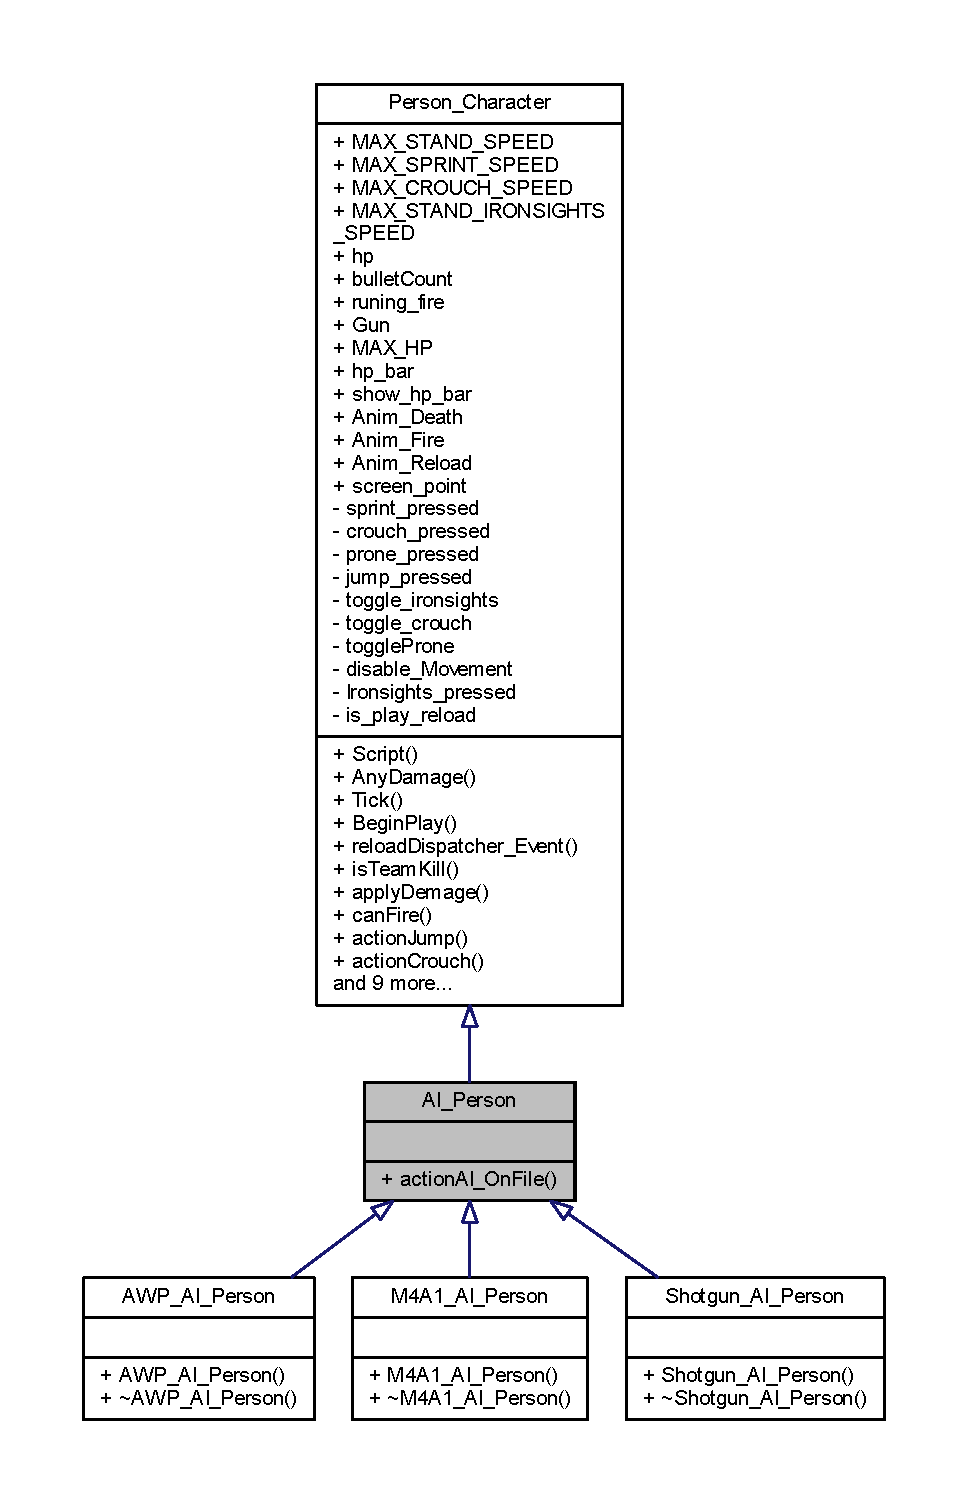
\includegraphics[height=550pt]{class_a_i___person__inherit__graph}
\end{center}
\end{figure}


Collaboration diagram for A\+I\+\_\+\+Person\+:\nopagebreak
\begin{figure}[H]
\begin{center}
\leavevmode
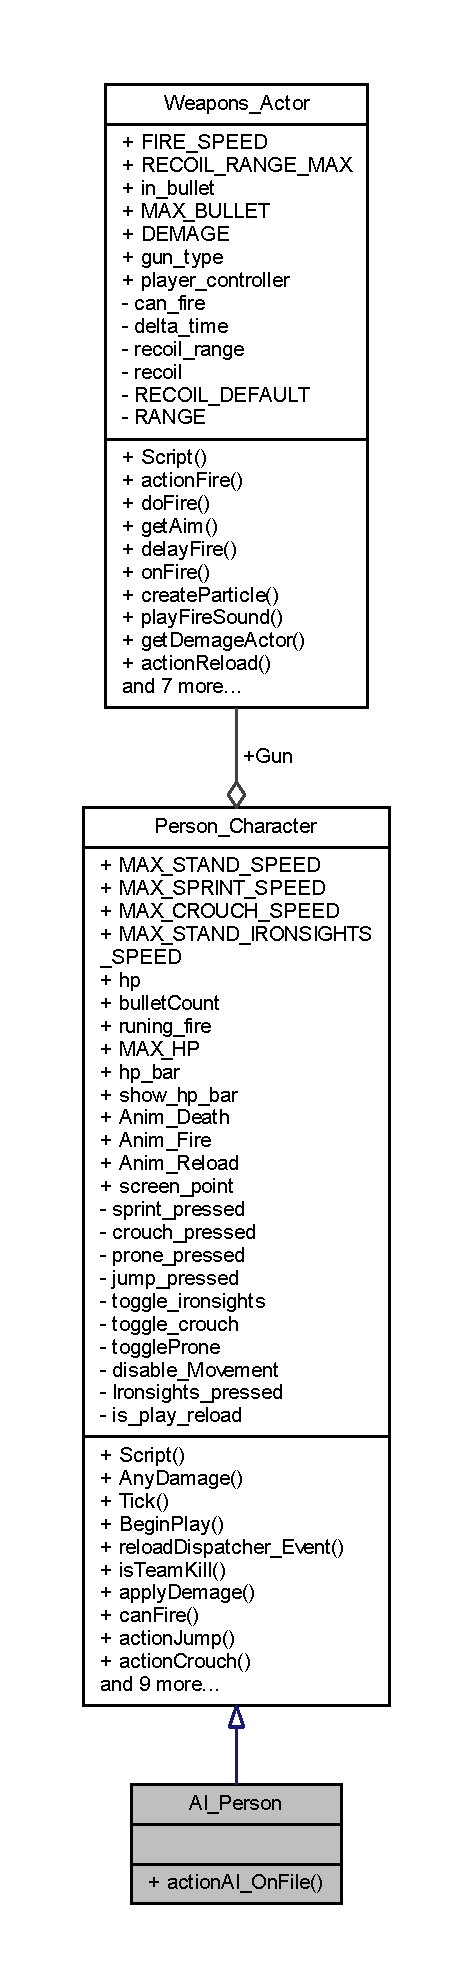
\includegraphics[height=550pt]{class_a_i___person__coll__graph}
\end{center}
\end{figure}
\subsection*{Public Member Functions}
\begin{DoxyCompactItemize}
\item 
Event\+Graph \hyperlink{class_a_i___person_a4d637f505caf3a5e7abf665986b5e8d2}{Tick} (float Delta\+Seconds)
\begin{DoxyCompactList}\small\item\em Tick 이벤트. \end{DoxyCompactList}\item 
void \hyperlink{class_a_i___person_aa6625ce68ebad8cdc678c872f41b5944}{action\+A\+I\+\_\+\+On\+File} (float \+\_\+delta\+\_\+seconds, Vector \+\_\+end\+\_\+location, Object \+\_\+get\+\_\+object)
\begin{DoxyCompactList}\small\item\em 사격 명령이 들어옴. \end{DoxyCompactList}\item 
void \hyperlink{class_a_i___person_a21ffa62d7f7c59a7c8a496c5012ef721}{action\+A\+I\+\_\+\+Reload} ()
\begin{DoxyCompactList}\small\item\em 재장전 \end{DoxyCompactList}\end{DoxyCompactItemize}
\subsection*{Additional Inherited Members}


\subsection{Detailed Description}
AI 팀원 클래스. 

.... 

\subsection{Member Function Documentation}
\index{A\+I\+\_\+\+Person@{A\+I\+\_\+\+Person}!action\+A\+I\+\_\+\+On\+File@{action\+A\+I\+\_\+\+On\+File}}
\index{action\+A\+I\+\_\+\+On\+File@{action\+A\+I\+\_\+\+On\+File}!A\+I\+\_\+\+Person@{A\+I\+\_\+\+Person}}
\subsubsection[{\texorpdfstring{action\+A\+I\+\_\+\+On\+File(float \+\_\+delta\+\_\+seconds, Vector \+\_\+end\+\_\+location, Object \+\_\+get\+\_\+object)}{actionAI_OnFile(float _delta_seconds, Vector _end_location, Object _get_object)}}]{\setlength{\rightskip}{0pt plus 5cm}void A\+I\+\_\+\+Person\+::action\+A\+I\+\_\+\+On\+File (
\begin{DoxyParamCaption}
\item[{float}]{\+\_\+delta\+\_\+seconds, }
\item[{Vector}]{\+\_\+end\+\_\+location, }
\item[{Object}]{\+\_\+get\+\_\+object}
\end{DoxyParamCaption}
)}\hypertarget{class_a_i___person_aa6625ce68ebad8cdc678c872f41b5944}{}\label{class_a_i___person_aa6625ce68ebad8cdc678c872f41b5944}


사격 명령이 들어옴. 

AI 처리 블루프린트에서 사격 명령(이벤트)를 실행. 
\begin{DoxyParams}{Parameters}
{\em \+\_\+delta\+\_\+seconds} & 프레임간 시간 간격 \\
\hline
{\em \+\_\+end\+\_\+location} & 사격 포인트 \\
\hline
{\em \+\_\+get\+\_\+object} & 사격대상 \\
\hline
\end{DoxyParams}


Here is the call graph for this function\+:\nopagebreak
\begin{figure}[H]
\begin{center}
\leavevmode
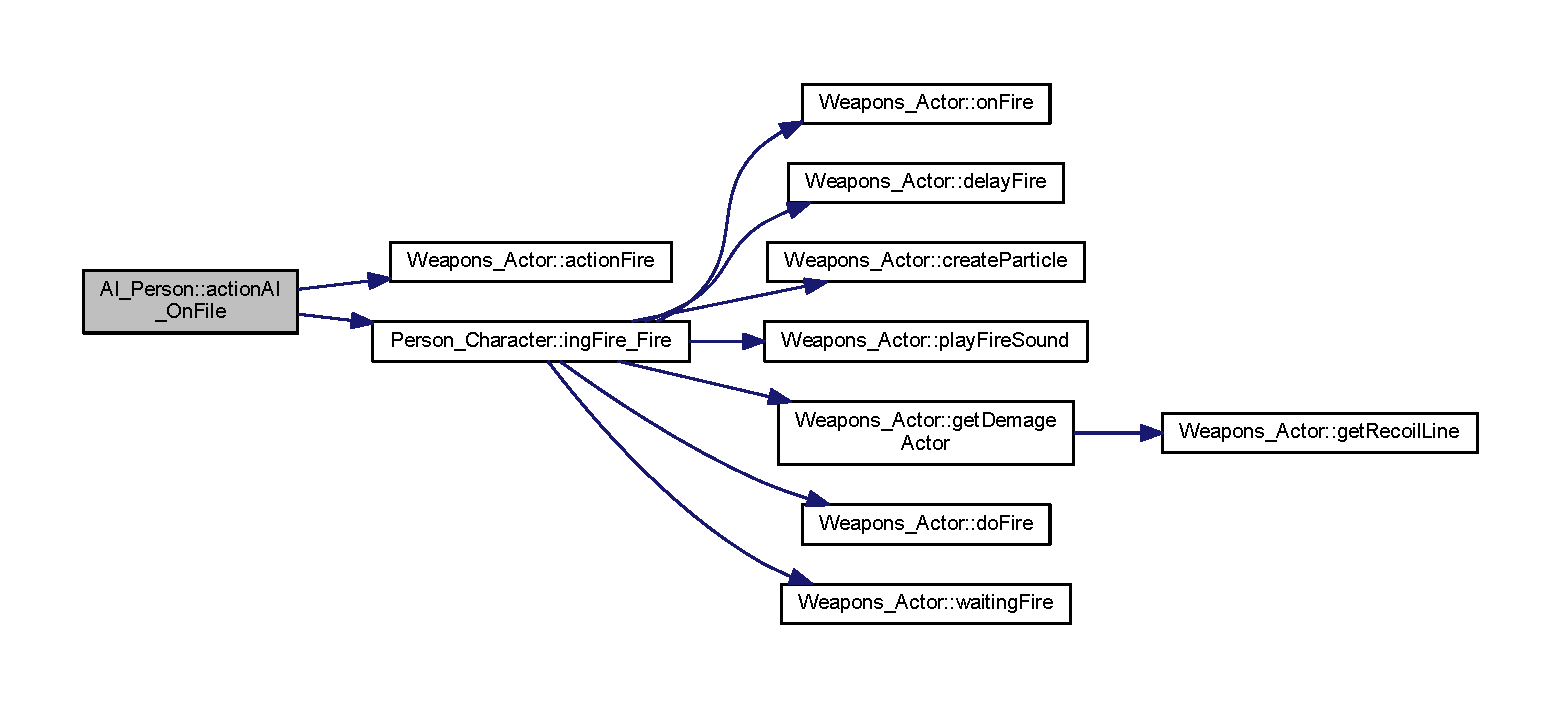
\includegraphics[width=350pt]{class_a_i___person_aa6625ce68ebad8cdc678c872f41b5944_cgraph}
\end{center}
\end{figure}


\index{A\+I\+\_\+\+Person@{A\+I\+\_\+\+Person}!action\+A\+I\+\_\+\+Reload@{action\+A\+I\+\_\+\+Reload}}
\index{action\+A\+I\+\_\+\+Reload@{action\+A\+I\+\_\+\+Reload}!A\+I\+\_\+\+Person@{A\+I\+\_\+\+Person}}
\subsubsection[{\texorpdfstring{action\+A\+I\+\_\+\+Reload()}{actionAI_Reload()}}]{\setlength{\rightskip}{0pt plus 5cm}void A\+I\+\_\+\+Person\+::action\+A\+I\+\_\+\+Reload (
\begin{DoxyParamCaption}
{}
\end{DoxyParamCaption}
)}\hypertarget{class_a_i___person_a21ffa62d7f7c59a7c8a496c5012ef721}{}\label{class_a_i___person_a21ffa62d7f7c59a7c8a496c5012ef721}


재장전 



Here is the call graph for this function\+:\nopagebreak
\begin{figure}[H]
\begin{center}
\leavevmode
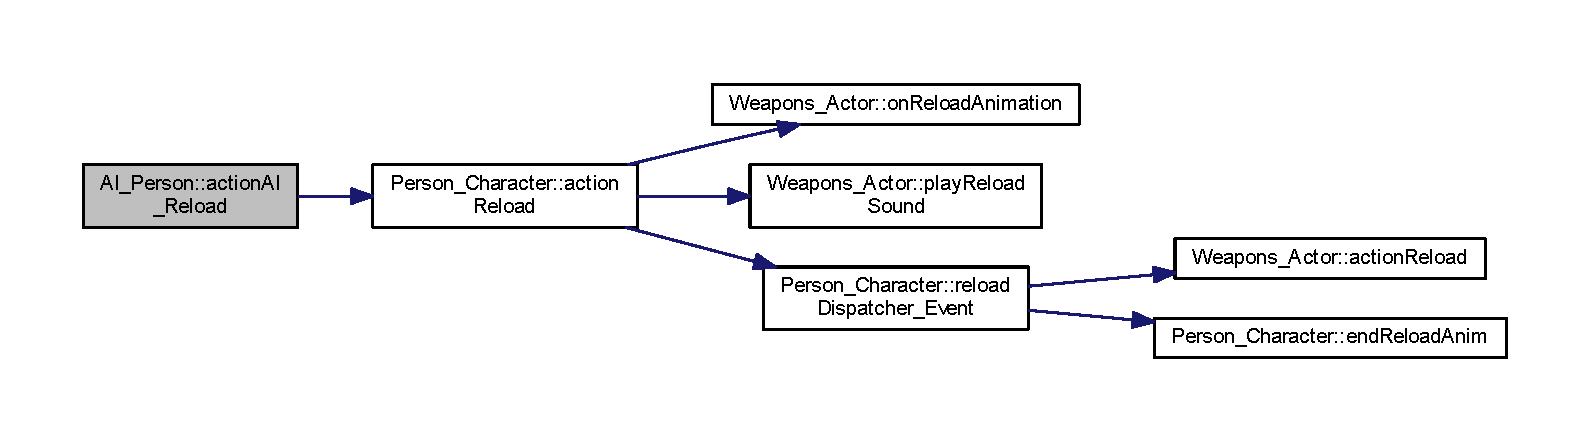
\includegraphics[width=350pt]{class_a_i___person_a21ffa62d7f7c59a7c8a496c5012ef721_cgraph}
\end{center}
\end{figure}


\index{A\+I\+\_\+\+Person@{A\+I\+\_\+\+Person}!Tick@{Tick}}
\index{Tick@{Tick}!A\+I\+\_\+\+Person@{A\+I\+\_\+\+Person}}
\subsubsection[{\texorpdfstring{Tick(float Delta\+Seconds)}{Tick(float DeltaSeconds)}}]{\setlength{\rightskip}{0pt plus 5cm}Event\+Graph A\+I\+\_\+\+Person\+::\+Tick (
\begin{DoxyParamCaption}
\item[{float}]{Delta\+Seconds}
\end{DoxyParamCaption}
)}\hypertarget{class_a_i___person_a4d637f505caf3a5e7abf665986b5e8d2}{}\label{class_a_i___person_a4d637f505caf3a5e7abf665986b5e8d2}


Tick 이벤트. 

매 프레임마다 실행되는 이벤트.

총을 쏘고 있는 중인지 체크한다.

디버깅용 Hp Bar를 표시한다. 
\begin{DoxyParams}[1]{Parameters}
\textquotesingle{}https\+://docs.\+unrealengine.\+com/latest/\+K\+O\+R/\+Engine/\+Blueprints/\+User\+Guide/\+Events/index.\+html & {\em eventtick\textquotesingle{}} & \\
\hline
\end{DoxyParams}


Here is the call graph for this function\+:\nopagebreak
\begin{figure}[H]
\begin{center}
\leavevmode
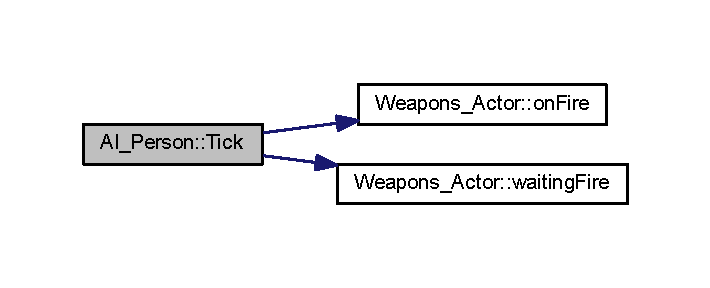
\includegraphics[width=341pt]{class_a_i___person_a4d637f505caf3a5e7abf665986b5e8d2_cgraph}
\end{center}
\end{figure}



\hypertarget{class_all___a_i_controller}{}\section{All\+\_\+\+A\+I\+Controller Class Reference}
\label{class_all___a_i_controller}\index{All\+\_\+\+A\+I\+Controller@{All\+\_\+\+A\+I\+Controller}}


팀원 AI 컨트롤러  




{\ttfamily \#include $<$All\+\_\+\+A\+I\+Controller.\+h$>$}



Inheritance diagram for All\+\_\+\+A\+I\+Controller\+:\nopagebreak
\begin{figure}[H]
\begin{center}
\leavevmode
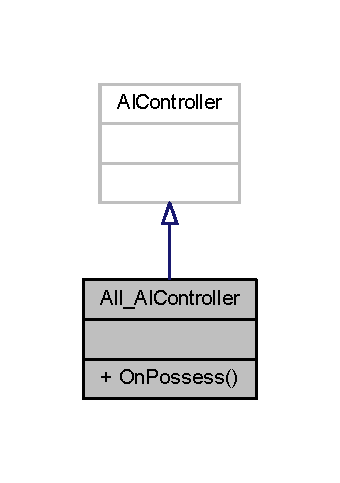
\includegraphics[width=163pt]{class_all___a_i_controller__inherit__graph}
\end{center}
\end{figure}


Collaboration diagram for All\+\_\+\+A\+I\+Controller\+:\nopagebreak
\begin{figure}[H]
\begin{center}
\leavevmode
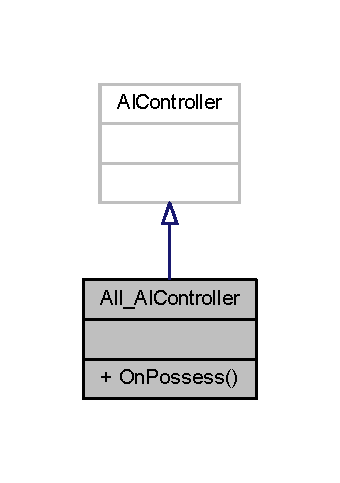
\includegraphics[width=163pt]{class_all___a_i_controller__coll__graph}
\end{center}
\end{figure}
\subsection*{Public Member Functions}
\begin{DoxyCompactItemize}
\item 
Event\+Graph \hyperlink{class_all___a_i_controller_a544dad6036ff558c32ac4b7622877bcb}{On\+Possess} ()
\begin{DoxyCompactList}\small\item\em Possess 이벤트 \end{DoxyCompactList}\end{DoxyCompactItemize}


\subsection{Detailed Description}
팀원 AI 컨트롤러 

팀원 AI 캐릭터들을 컨트롤하기 위한 프레임워크 애셋 

\subsection{Member Function Documentation}
\index{All\+\_\+\+A\+I\+Controller@{All\+\_\+\+A\+I\+Controller}!On\+Possess@{On\+Possess}}
\index{On\+Possess@{On\+Possess}!All\+\_\+\+A\+I\+Controller@{All\+\_\+\+A\+I\+Controller}}
\subsubsection[{\texorpdfstring{On\+Possess()}{OnPossess()}}]{\setlength{\rightskip}{0pt plus 5cm}Event\+Graph All\+\_\+\+A\+I\+Controller\+::\+On\+Possess (
\begin{DoxyParamCaption}
{}
\end{DoxyParamCaption}
)}\hypertarget{class_all___a_i_controller_a544dad6036ff558c32ac4b7622877bcb}{}\label{class_all___a_i_controller_a544dad6036ff558c32ac4b7622877bcb}


Possess 이벤트 

팀원 AI 비헤이비어 트리를 각각의 팀원 캐릭터들에게 연결시켜준다. 
\hypertarget{class_approach___b_t_task}{}\section{Approach\+\_\+\+B\+T\+Task Class Reference}
\label{class_approach___b_t_task}\index{Approach\+\_\+\+B\+T\+Task@{Approach\+\_\+\+B\+T\+Task}}


적 AI 태스크  




{\ttfamily \#include $<$Approach\+\_\+\+B\+T\+Task.\+h$>$}



Inheritance diagram for Approach\+\_\+\+B\+T\+Task\+:
\nopagebreak
\begin{figure}[H]
\begin{center}
\leavevmode
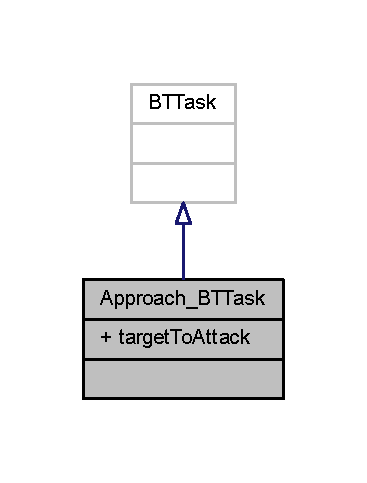
\includegraphics[width=181pt]{class_approach___b_t_task__inherit__graph}
\end{center}
\end{figure}


Collaboration diagram for Approach\+\_\+\+B\+T\+Task\+:
\nopagebreak
\begin{figure}[H]
\begin{center}
\leavevmode
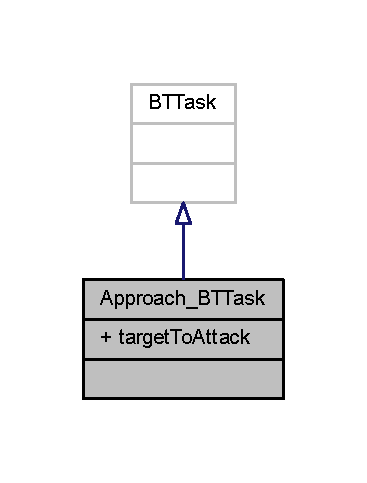
\includegraphics[width=181pt]{class_approach___b_t_task__coll__graph}
\end{center}
\end{figure}
\subsection*{Public Member Functions}
\begin{DoxyCompactItemize}
\item 
Event\+Graph \hyperlink{class_approach___b_t_task_aab5432bc101b98aaed56ed2880688a14}{Receive\+Execute} (Actor Owner\+Actor)
\begin{DoxyCompactList}\small\item\em 태스크 실행 이벤트 \end{DoxyCompactList}\end{DoxyCompactItemize}
\subsection*{Public Attributes}
\begin{DoxyCompactItemize}
\item 
Blackboard\+Key\+Selector \hyperlink{class_approach___b_t_task_a0af1525e9ae6377da4fecc32e1dfe5f3}{target\+To\+Attack}
\end{DoxyCompactItemize}


\subsection{Detailed Description}
적 AI 태스크 

공격하려는 대상에게 접근하는 기능을 한다. 

\subsection{Member Function Documentation}
\index{Approach\+\_\+\+B\+T\+Task@{Approach\+\_\+\+B\+T\+Task}!Receive\+Execute@{Receive\+Execute}}
\index{Receive\+Execute@{Receive\+Execute}!Approach\+\_\+\+B\+T\+Task@{Approach\+\_\+\+B\+T\+Task}}
\subsubsection[{\texorpdfstring{Receive\+Execute(\+Actor Owner\+Actor)}{ReceiveExecute(Actor OwnerActor)}}]{\setlength{\rightskip}{0pt plus 5cm}Event\+Graph Approach\+\_\+\+B\+T\+Task\+::\+Receive\+Execute (
\begin{DoxyParamCaption}
\item[{Actor}]{Owner\+Actor}
\end{DoxyParamCaption}
)}\hypertarget{class_approach___b_t_task_aab5432bc101b98aaed56ed2880688a14}{}\label{class_approach___b_t_task_aab5432bc101b98aaed56ed2880688a14}


태스크 실행 이벤트 

AI 컨트롤러가 컨트롤하는 폰을 공격할 대상의 위치로 이동시킨다. 
\begin{DoxyParams}{Parameters}
{\em Owner\+Actor} & AI 컨트롤러. \\
\hline
\end{DoxyParams}


Here is the caller graph for this function\+:
\nopagebreak
\begin{figure}[H]
\begin{center}
\leavevmode
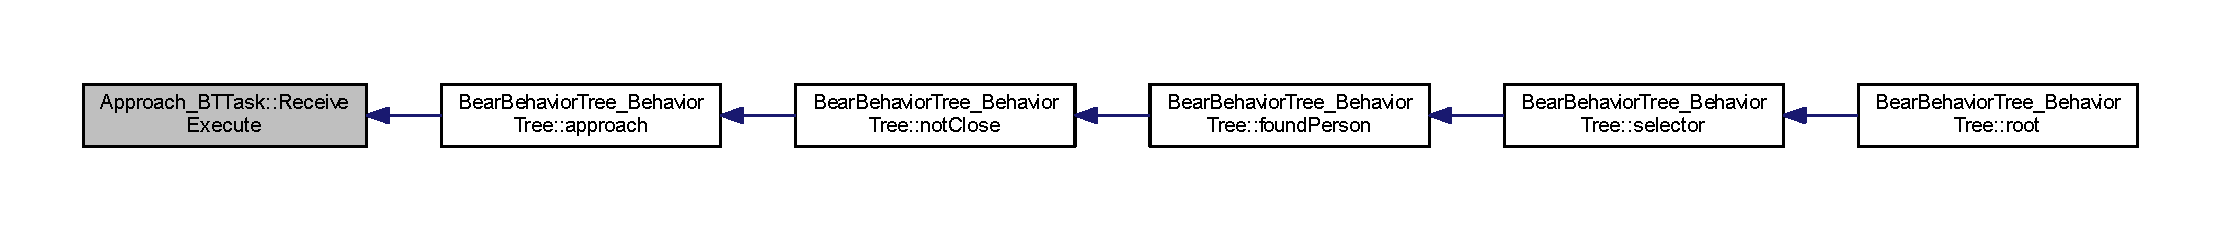
\includegraphics[width=350pt]{class_approach___b_t_task_aab5432bc101b98aaed56ed2880688a14_icgraph}
\end{center}
\end{figure}




\subsection{Member Data Documentation}
\index{Approach\+\_\+\+B\+T\+Task@{Approach\+\_\+\+B\+T\+Task}!target\+To\+Attack@{target\+To\+Attack}}
\index{target\+To\+Attack@{target\+To\+Attack}!Approach\+\_\+\+B\+T\+Task@{Approach\+\_\+\+B\+T\+Task}}
\subsubsection[{\texorpdfstring{target\+To\+Attack}{targetToAttack}}]{\setlength{\rightskip}{0pt plus 5cm}Blackboard\+Key\+Selector Approach\+\_\+\+B\+T\+Task\+::target\+To\+Attack}\hypertarget{class_approach___b_t_task_a0af1525e9ae6377da4fecc32e1dfe5f3}{}\label{class_approach___b_t_task_a0af1525e9ae6377da4fecc32e1dfe5f3}

\hypertarget{class_a_w_p___a_i___person}{}\section{A\+W\+P\+\_\+\+A\+I\+\_\+\+Person Class Reference}
\label{class_a_w_p___a_i___person}\index{A\+W\+P\+\_\+\+A\+I\+\_\+\+Person@{A\+W\+P\+\_\+\+A\+I\+\_\+\+Person}}


AI 팀원 중 스나이퍼에 알맞게 설정.  




{\ttfamily \#include $<$A\+W\+P\+\_\+\+A\+I\+\_\+\+Person.\+h$>$}



Inheritance diagram for A\+W\+P\+\_\+\+A\+I\+\_\+\+Person\+:
\nopagebreak
\begin{figure}[H]
\begin{center}
\leavevmode
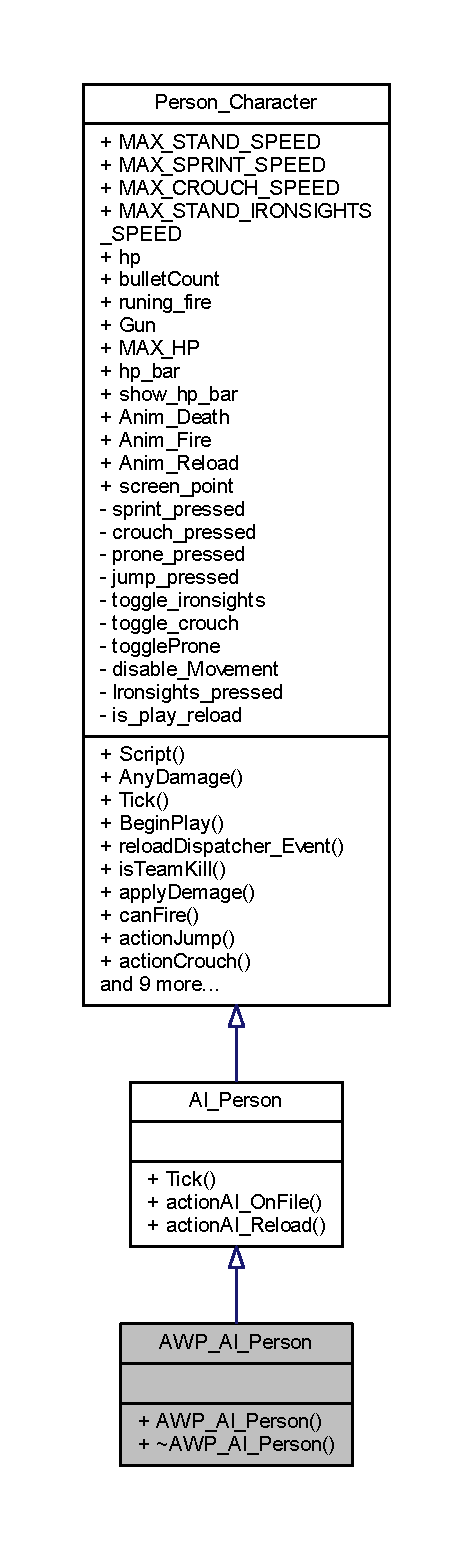
\includegraphics[height=550pt]{class_a_w_p___a_i___person__inherit__graph}
\end{center}
\end{figure}


Collaboration diagram for A\+W\+P\+\_\+\+A\+I\+\_\+\+Person\+:
\nopagebreak
\begin{figure}[H]
\begin{center}
\leavevmode
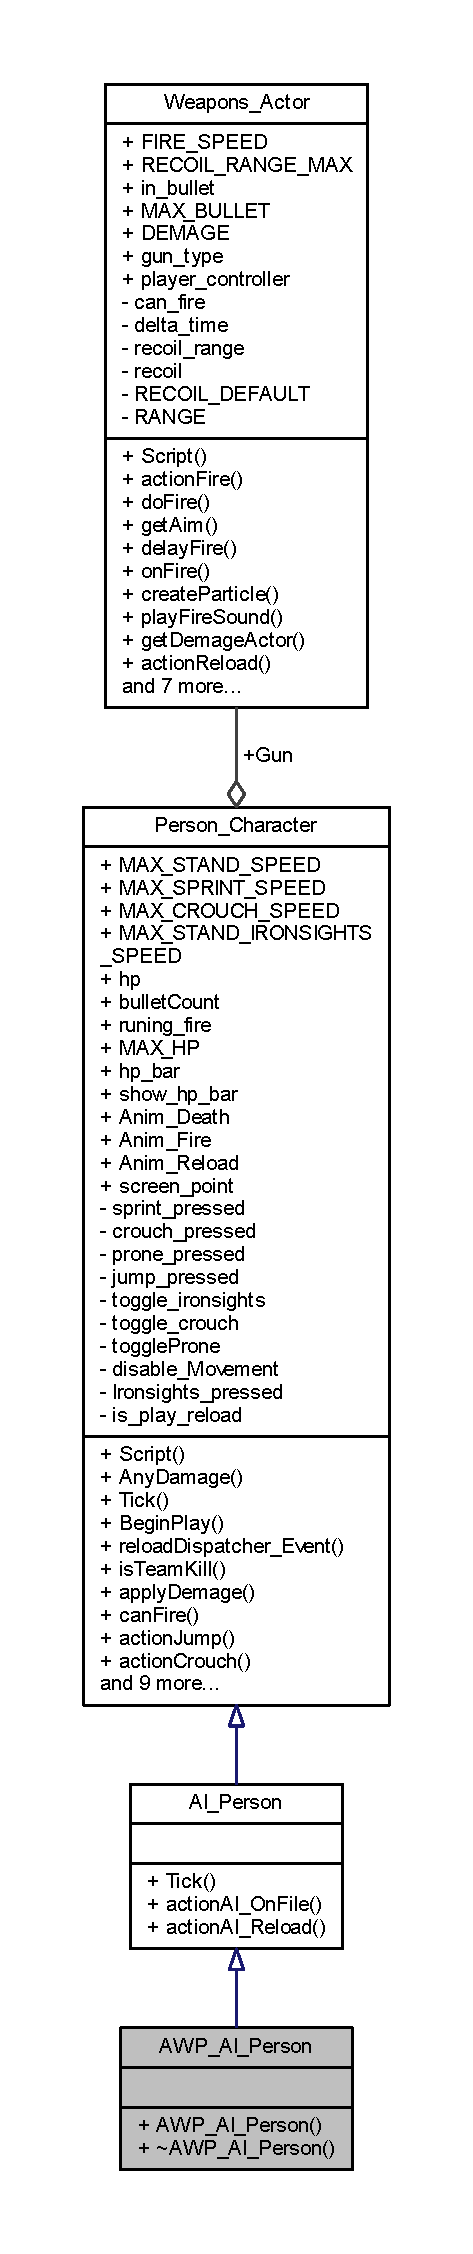
\includegraphics[height=550pt]{class_a_w_p___a_i___person__coll__graph}
\end{center}
\end{figure}
\subsection*{Additional Inherited Members}


\subsection{Detailed Description}
AI 팀원 중 스나이퍼에 알맞게 설정. 

.... 
\hypertarget{class_a_w_p___weapons}{}\section{A\+W\+P\+\_\+\+Weapons Class Reference}
\label{class_a_w_p___weapons}\index{A\+W\+P\+\_\+\+Weapons@{A\+W\+P\+\_\+\+Weapons}}


{\ttfamily \#include $<$A\+W\+P\+\_\+\+Weapons.\+h$>$}



Inheritance diagram for A\+W\+P\+\_\+\+Weapons\+:\nopagebreak
\begin{figure}[H]
\begin{center}
\leavevmode
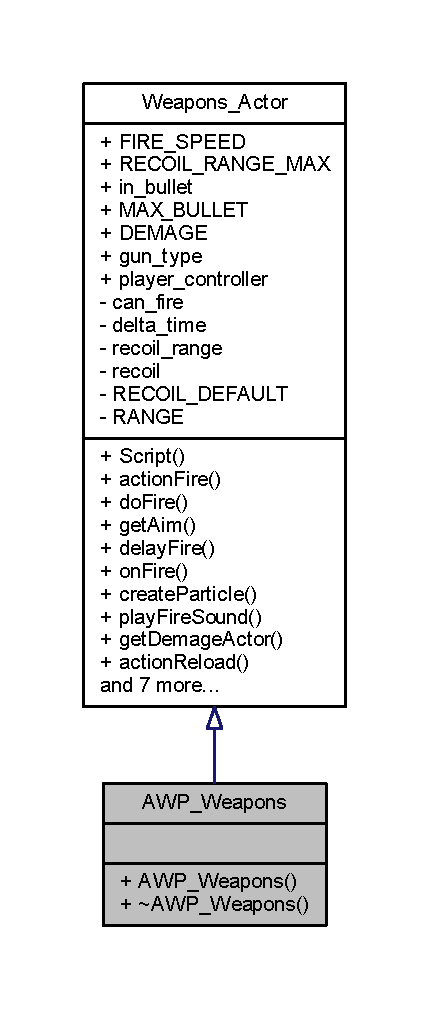
\includegraphics[width=206pt]{class_a_w_p___weapons__inherit__graph}
\end{center}
\end{figure}


Collaboration diagram for A\+W\+P\+\_\+\+Weapons\+:\nopagebreak
\begin{figure}[H]
\begin{center}
\leavevmode
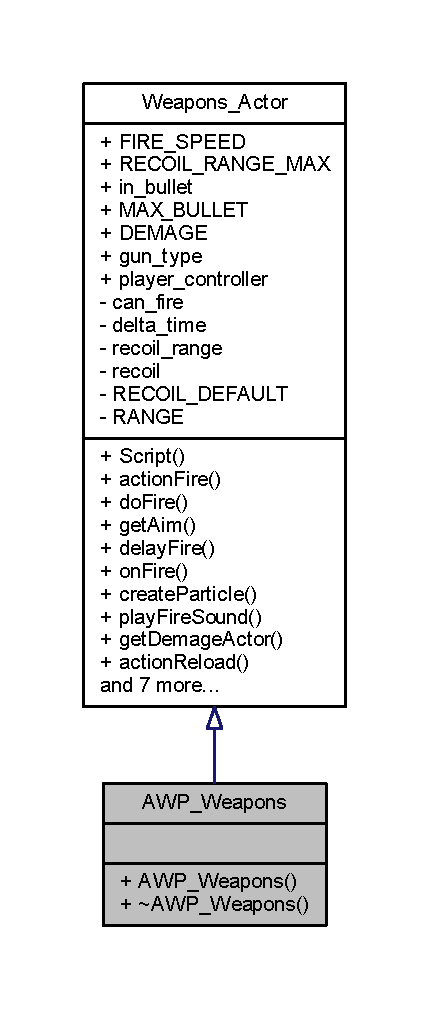
\includegraphics[width=206pt]{class_a_w_p___weapons__coll__graph}
\end{center}
\end{figure}
\subsection*{Public Member Functions}
\begin{DoxyCompactItemize}
\item 
\hyperlink{class_a_w_p___weapons_a4aa9feddb05fde14748dca413e3b9147}{A\+W\+P\+\_\+\+Weapons} ()
\item 
\hyperlink{class_a_w_p___weapons_a0c44fa46d60b22c5d6d3607dd1979934}{$\sim$\+A\+W\+P\+\_\+\+Weapons} ()
\end{DoxyCompactItemize}
\subsection*{Additional Inherited Members}


\subsection{Constructor \& Destructor Documentation}
\index{A\+W\+P\+\_\+\+Weapons@{A\+W\+P\+\_\+\+Weapons}!A\+W\+P\+\_\+\+Weapons@{A\+W\+P\+\_\+\+Weapons}}
\index{A\+W\+P\+\_\+\+Weapons@{A\+W\+P\+\_\+\+Weapons}!A\+W\+P\+\_\+\+Weapons@{A\+W\+P\+\_\+\+Weapons}}
\subsubsection[{\texorpdfstring{A\+W\+P\+\_\+\+Weapons()}{AWP_Weapons()}}]{\setlength{\rightskip}{0pt plus 5cm}A\+W\+P\+\_\+\+Weapons\+::\+A\+W\+P\+\_\+\+Weapons (
\begin{DoxyParamCaption}
{}
\end{DoxyParamCaption}
)}\hypertarget{class_a_w_p___weapons_a4aa9feddb05fde14748dca413e3b9147}{}\label{class_a_w_p___weapons_a4aa9feddb05fde14748dca413e3b9147}
\index{A\+W\+P\+\_\+\+Weapons@{A\+W\+P\+\_\+\+Weapons}!````~A\+W\+P\+\_\+\+Weapons@{$\sim$\+A\+W\+P\+\_\+\+Weapons}}
\index{````~A\+W\+P\+\_\+\+Weapons@{$\sim$\+A\+W\+P\+\_\+\+Weapons}!A\+W\+P\+\_\+\+Weapons@{A\+W\+P\+\_\+\+Weapons}}
\subsubsection[{\texorpdfstring{$\sim$\+A\+W\+P\+\_\+\+Weapons()}{~AWP_Weapons()}}]{\setlength{\rightskip}{0pt plus 5cm}A\+W\+P\+\_\+\+Weapons\+::$\sim$\+A\+W\+P\+\_\+\+Weapons (
\begin{DoxyParamCaption}
{}
\end{DoxyParamCaption}
)}\hypertarget{class_a_w_p___weapons_a0c44fa46d60b22c5d6d3607dd1979934}{}\label{class_a_w_p___weapons_a0c44fa46d60b22c5d6d3607dd1979934}

\hypertarget{class_b_b___humen}{}\section{B\+B\+\_\+\+Humen Class Reference}
\label{class_b_b___humen}\index{B\+B\+\_\+\+Humen@{B\+B\+\_\+\+Humen}}


팀원 AI 블랙보드  




{\ttfamily \#include $<$B\+B\+\_\+\+Humen.\+h$>$}



Inheritance diagram for B\+B\+\_\+\+Humen\+:
\nopagebreak
\begin{figure}[H]
\begin{center}
\leavevmode
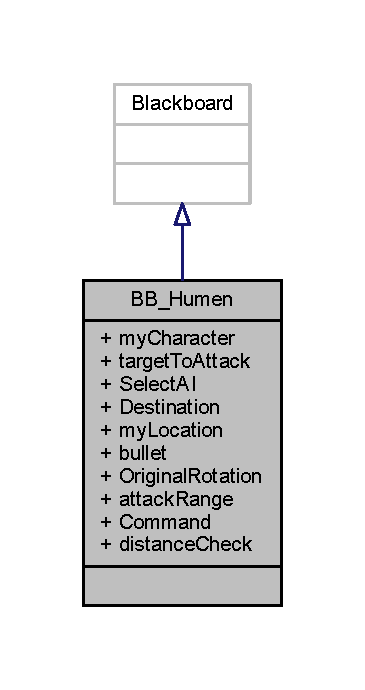
\includegraphics[width=175pt]{class_b_b___humen__inherit__graph}
\end{center}
\end{figure}


Collaboration diagram for B\+B\+\_\+\+Humen\+:
\nopagebreak
\begin{figure}[H]
\begin{center}
\leavevmode
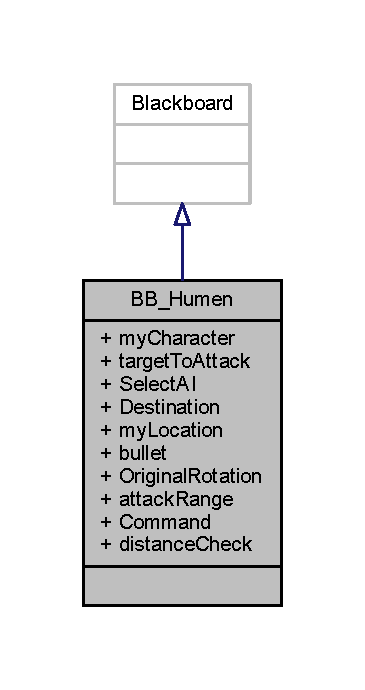
\includegraphics[width=175pt]{class_b_b___humen__coll__graph}
\end{center}
\end{figure}
\subsection*{Public Attributes}
\begin{DoxyCompactItemize}
\item 
Object \hyperlink{class_b_b___humen_a7f9491363e6d98dd20be54751e78c76b}{my\+Character}
\item 
Object \hyperlink{class_b_b___humen_a4d3316519116e095dd0b34472b5f24d4}{target\+To\+Attack}
\item 
Object \hyperlink{class_b_b___humen_a6a1bca9746fc00983e69bc821ccdeda7}{Select\+AI}
\item 
Vector \hyperlink{class_b_b___humen_a52f772a3da5b3c23c6ff239571573a10}{Destination}
\item 
Vector \hyperlink{class_b_b___humen_a135f2ee9b81ee3285d27e52ecf2c147c}{my\+Location}
\item 
Integer \hyperlink{class_b_b___humen_a87f003bcd85b60d96e6ef1ebab51976e}{bullet}
\item 
Rotator \hyperlink{class_b_b___humen_af8860690e8fc6772d27a923223e424ec}{Original\+Rotation}
\item 
Float \hyperlink{class_b_b___humen_a9fb506718878e67dd7ce4889188fd9c3}{attack\+Range}
\item 
Bool \hyperlink{class_b_b___humen_a5f3cc37acdcbf06281e92a1792354864}{Command}
\item 
Bool \hyperlink{class_b_b___humen_a4f067f9c00145461036a0419a631dd06}{distance\+Check}
\end{DoxyCompactItemize}


\subsection{Detailed Description}
팀원 AI 블랙보드 

비헤이비어 트리의 흐름을 제어하기 위한 변수들을 모아두는 곳이다. 

\subsection{Member Data Documentation}
\index{B\+B\+\_\+\+Humen@{B\+B\+\_\+\+Humen}!attack\+Range@{attack\+Range}}
\index{attack\+Range@{attack\+Range}!B\+B\+\_\+\+Humen@{B\+B\+\_\+\+Humen}}
\subsubsection[{\texorpdfstring{attack\+Range}{attackRange}}]{\setlength{\rightskip}{0pt plus 5cm}Float B\+B\+\_\+\+Humen\+::attack\+Range}\hypertarget{class_b_b___humen_a9fb506718878e67dd7ce4889188fd9c3}{}\label{class_b_b___humen_a9fb506718878e67dd7ce4889188fd9c3}
\index{B\+B\+\_\+\+Humen@{B\+B\+\_\+\+Humen}!bullet@{bullet}}
\index{bullet@{bullet}!B\+B\+\_\+\+Humen@{B\+B\+\_\+\+Humen}}
\subsubsection[{\texorpdfstring{bullet}{bullet}}]{\setlength{\rightskip}{0pt plus 5cm}Integer B\+B\+\_\+\+Humen\+::bullet}\hypertarget{class_b_b___humen_a87f003bcd85b60d96e6ef1ebab51976e}{}\label{class_b_b___humen_a87f003bcd85b60d96e6ef1ebab51976e}
\index{B\+B\+\_\+\+Humen@{B\+B\+\_\+\+Humen}!Command@{Command}}
\index{Command@{Command}!B\+B\+\_\+\+Humen@{B\+B\+\_\+\+Humen}}
\subsubsection[{\texorpdfstring{Command}{Command}}]{\setlength{\rightskip}{0pt plus 5cm}Bool B\+B\+\_\+\+Humen\+::\+Command}\hypertarget{class_b_b___humen_a5f3cc37acdcbf06281e92a1792354864}{}\label{class_b_b___humen_a5f3cc37acdcbf06281e92a1792354864}
\index{B\+B\+\_\+\+Humen@{B\+B\+\_\+\+Humen}!Destination@{Destination}}
\index{Destination@{Destination}!B\+B\+\_\+\+Humen@{B\+B\+\_\+\+Humen}}
\subsubsection[{\texorpdfstring{Destination}{Destination}}]{\setlength{\rightskip}{0pt plus 5cm}Vector B\+B\+\_\+\+Humen\+::\+Destination}\hypertarget{class_b_b___humen_a52f772a3da5b3c23c6ff239571573a10}{}\label{class_b_b___humen_a52f772a3da5b3c23c6ff239571573a10}
\index{B\+B\+\_\+\+Humen@{B\+B\+\_\+\+Humen}!distance\+Check@{distance\+Check}}
\index{distance\+Check@{distance\+Check}!B\+B\+\_\+\+Humen@{B\+B\+\_\+\+Humen}}
\subsubsection[{\texorpdfstring{distance\+Check}{distanceCheck}}]{\setlength{\rightskip}{0pt plus 5cm}Bool B\+B\+\_\+\+Humen\+::distance\+Check}\hypertarget{class_b_b___humen_a4f067f9c00145461036a0419a631dd06}{}\label{class_b_b___humen_a4f067f9c00145461036a0419a631dd06}
\index{B\+B\+\_\+\+Humen@{B\+B\+\_\+\+Humen}!my\+Character@{my\+Character}}
\index{my\+Character@{my\+Character}!B\+B\+\_\+\+Humen@{B\+B\+\_\+\+Humen}}
\subsubsection[{\texorpdfstring{my\+Character}{myCharacter}}]{\setlength{\rightskip}{0pt plus 5cm}Object B\+B\+\_\+\+Humen\+::my\+Character}\hypertarget{class_b_b___humen_a7f9491363e6d98dd20be54751e78c76b}{}\label{class_b_b___humen_a7f9491363e6d98dd20be54751e78c76b}
\index{B\+B\+\_\+\+Humen@{B\+B\+\_\+\+Humen}!my\+Location@{my\+Location}}
\index{my\+Location@{my\+Location}!B\+B\+\_\+\+Humen@{B\+B\+\_\+\+Humen}}
\subsubsection[{\texorpdfstring{my\+Location}{myLocation}}]{\setlength{\rightskip}{0pt plus 5cm}Vector B\+B\+\_\+\+Humen\+::my\+Location}\hypertarget{class_b_b___humen_a135f2ee9b81ee3285d27e52ecf2c147c}{}\label{class_b_b___humen_a135f2ee9b81ee3285d27e52ecf2c147c}
\index{B\+B\+\_\+\+Humen@{B\+B\+\_\+\+Humen}!Original\+Rotation@{Original\+Rotation}}
\index{Original\+Rotation@{Original\+Rotation}!B\+B\+\_\+\+Humen@{B\+B\+\_\+\+Humen}}
\subsubsection[{\texorpdfstring{Original\+Rotation}{OriginalRotation}}]{\setlength{\rightskip}{0pt plus 5cm}Rotator B\+B\+\_\+\+Humen\+::\+Original\+Rotation}\hypertarget{class_b_b___humen_af8860690e8fc6772d27a923223e424ec}{}\label{class_b_b___humen_af8860690e8fc6772d27a923223e424ec}
\index{B\+B\+\_\+\+Humen@{B\+B\+\_\+\+Humen}!Select\+AI@{Select\+AI}}
\index{Select\+AI@{Select\+AI}!B\+B\+\_\+\+Humen@{B\+B\+\_\+\+Humen}}
\subsubsection[{\texorpdfstring{Select\+AI}{SelectAI}}]{\setlength{\rightskip}{0pt plus 5cm}Object B\+B\+\_\+\+Humen\+::\+Select\+AI}\hypertarget{class_b_b___humen_a6a1bca9746fc00983e69bc821ccdeda7}{}\label{class_b_b___humen_a6a1bca9746fc00983e69bc821ccdeda7}
\index{B\+B\+\_\+\+Humen@{B\+B\+\_\+\+Humen}!target\+To\+Attack@{target\+To\+Attack}}
\index{target\+To\+Attack@{target\+To\+Attack}!B\+B\+\_\+\+Humen@{B\+B\+\_\+\+Humen}}
\subsubsection[{\texorpdfstring{target\+To\+Attack}{targetToAttack}}]{\setlength{\rightskip}{0pt plus 5cm}Object B\+B\+\_\+\+Humen\+::target\+To\+Attack}\hypertarget{class_b_b___humen_a4d3316519116e095dd0b34472b5f24d4}{}\label{class_b_b___humen_a4d3316519116e095dd0b34472b5f24d4}

\hypertarget{class_bear___enemy}{}\section{Bear\+\_\+\+Enemy Class Reference}
\label{class_bear___enemy}\index{Bear\+\_\+\+Enemy@{Bear\+\_\+\+Enemy}}


{\ttfamily \#include $<$Bear\+\_\+\+Enemy.\+h$>$}



Inheritance diagram for Bear\+\_\+\+Enemy\+:
\nopagebreak
\begin{figure}[H]
\begin{center}
\leavevmode
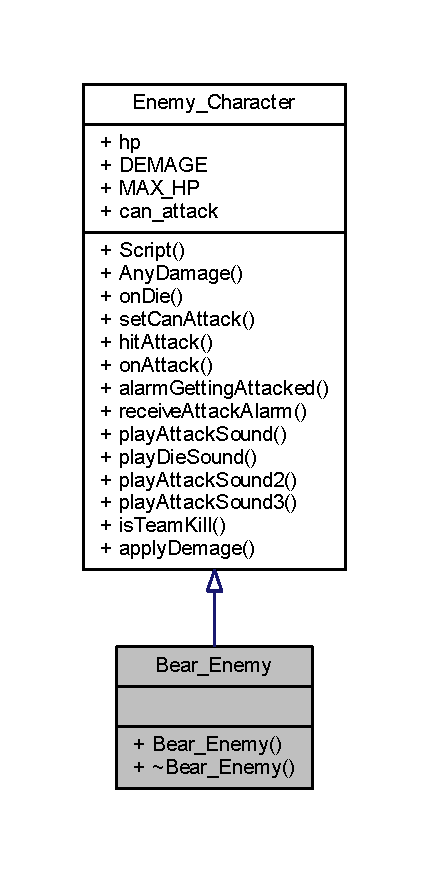
\includegraphics[width=206pt]{class_bear___enemy__inherit__graph}
\end{center}
\end{figure}


Collaboration diagram for Bear\+\_\+\+Enemy\+:
\nopagebreak
\begin{figure}[H]
\begin{center}
\leavevmode
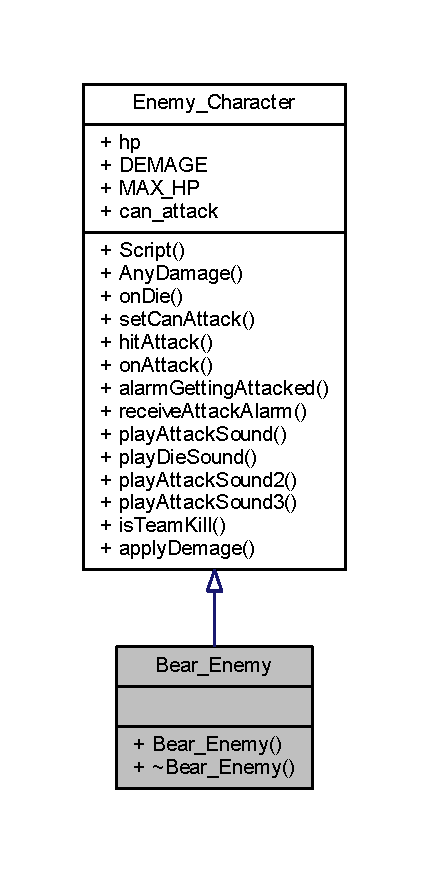
\includegraphics[width=206pt]{class_bear___enemy__coll__graph}
\end{center}
\end{figure}
\subsection*{Public Member Functions}
\begin{DoxyCompactItemize}
\item 
\hyperlink{class_bear___enemy_abac75b6766ef69ebd9fb6a661a67b307}{Bear\+\_\+\+Enemy} ()
\item 
\hyperlink{class_bear___enemy_abd0487f7f914f68ecccdadae2307e827}{$\sim$\+Bear\+\_\+\+Enemy} ()
\end{DoxyCompactItemize}
\subsection*{Additional Inherited Members}


\subsection{Constructor \& Destructor Documentation}
\index{Bear\+\_\+\+Enemy@{Bear\+\_\+\+Enemy}!Bear\+\_\+\+Enemy@{Bear\+\_\+\+Enemy}}
\index{Bear\+\_\+\+Enemy@{Bear\+\_\+\+Enemy}!Bear\+\_\+\+Enemy@{Bear\+\_\+\+Enemy}}
\subsubsection[{\texorpdfstring{Bear\+\_\+\+Enemy()}{Bear_Enemy()}}]{\setlength{\rightskip}{0pt plus 5cm}Bear\+\_\+\+Enemy\+::\+Bear\+\_\+\+Enemy (
\begin{DoxyParamCaption}
{}
\end{DoxyParamCaption}
)}\hypertarget{class_bear___enemy_abac75b6766ef69ebd9fb6a661a67b307}{}\label{class_bear___enemy_abac75b6766ef69ebd9fb6a661a67b307}
\index{Bear\+\_\+\+Enemy@{Bear\+\_\+\+Enemy}!````~Bear\+\_\+\+Enemy@{$\sim$\+Bear\+\_\+\+Enemy}}
\index{````~Bear\+\_\+\+Enemy@{$\sim$\+Bear\+\_\+\+Enemy}!Bear\+\_\+\+Enemy@{Bear\+\_\+\+Enemy}}
\subsubsection[{\texorpdfstring{$\sim$\+Bear\+\_\+\+Enemy()}{~Bear_Enemy()}}]{\setlength{\rightskip}{0pt plus 5cm}Bear\+\_\+\+Enemy\+::$\sim$\+Bear\+\_\+\+Enemy (
\begin{DoxyParamCaption}
{}
\end{DoxyParamCaption}
)}\hypertarget{class_bear___enemy_abd0487f7f914f68ecccdadae2307e827}{}\label{class_bear___enemy_abd0487f7f914f68ecccdadae2307e827}

\hypertarget{class_bear_behavior_tree___behavior_tree}{}\section{Bear\+Behavior\+Tree\+\_\+\+Behavior\+Tree Class Reference}
\label{class_bear_behavior_tree___behavior_tree}\index{Bear\+Behavior\+Tree\+\_\+\+Behavior\+Tree@{Bear\+Behavior\+Tree\+\_\+\+Behavior\+Tree}}


곰의 비헤이비어 트리  




{\ttfamily \#include $<$Bear\+Behavior\+Tree\+\_\+\+Behavior\+Tree.\+h$>$}



Inheritance diagram for Bear\+Behavior\+Tree\+\_\+\+Behavior\+Tree\+:\nopagebreak
\begin{figure}[H]
\begin{center}
\leavevmode
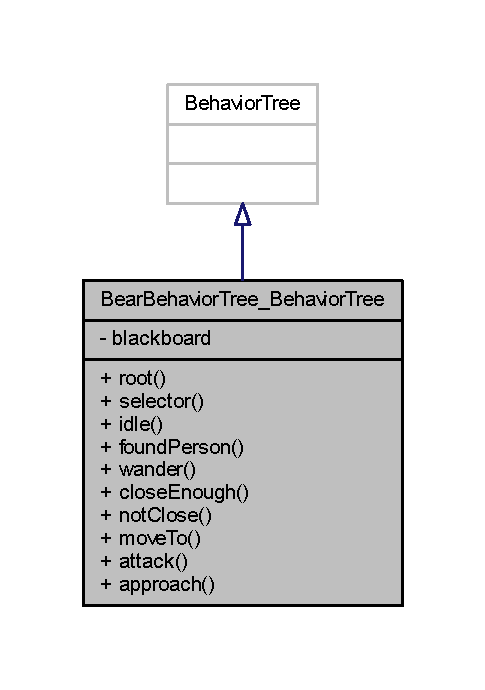
\includegraphics[width=233pt]{class_bear_behavior_tree___behavior_tree__inherit__graph}
\end{center}
\end{figure}


Collaboration diagram for Bear\+Behavior\+Tree\+\_\+\+Behavior\+Tree\+:\nopagebreak
\begin{figure}[H]
\begin{center}
\leavevmode
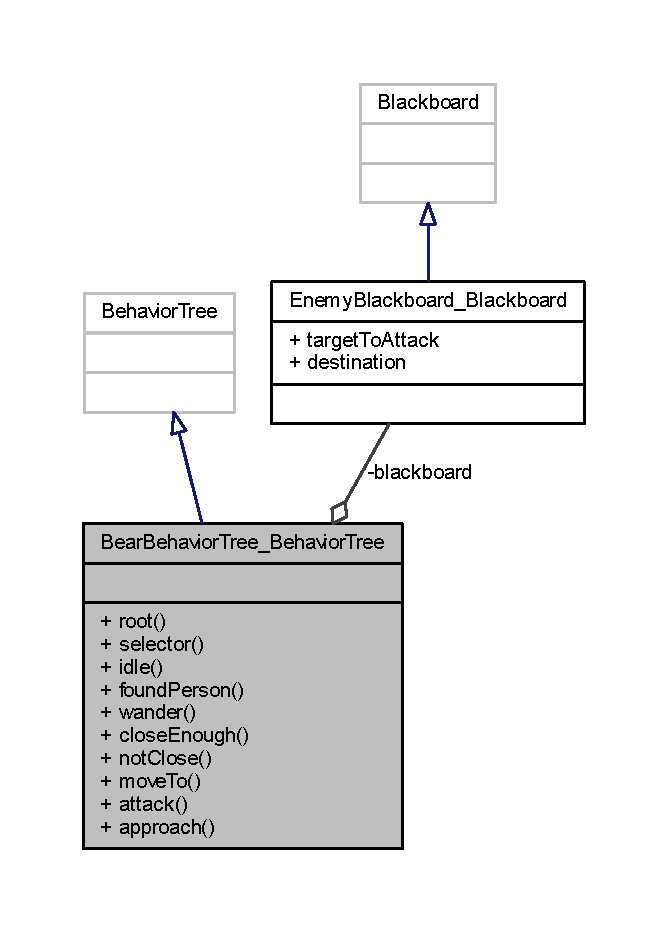
\includegraphics[width=321pt]{class_bear_behavior_tree___behavior_tree__coll__graph}
\end{center}
\end{figure}
\subsection*{Public Member Functions}
\begin{DoxyCompactItemize}
\item 
void \hyperlink{class_bear_behavior_tree___behavior_tree_a67e899c19fdc37eb5ed077d882ae4ad1}{root} (\hyperlink{class_enemy_blackboard___blackboard}{Enemy\+Blackboard\+\_\+\+Blackboard} \hyperlink{class_bear_behavior_tree___behavior_tree_af65805184758188534eb2100723629d7}{blackboard})
\begin{DoxyCompactList}\small\item\em 루트 노드 \end{DoxyCompactList}\item 
void \hyperlink{class_bear_behavior_tree___behavior_tree_a1d4c26a6c9f2c056a5d07f956129ba19}{selector} (Object target\+To\+Attack, Vector destination)
\begin{DoxyCompactList}\small\item\em 서비스를 가지는 분기 노드 \end{DoxyCompactList}\item 
void \hyperlink{class_bear_behavior_tree___behavior_tree_af17627dd1013988585a7afec3e36b00b}{idle} (Object target\+To\+Attack)
\begin{DoxyCompactList}\small\item\em 대기 상태 데코레이터 \end{DoxyCompactList}\item 
void \hyperlink{class_bear_behavior_tree___behavior_tree_a13134307abf8a5c1f0edef371b78f40b}{found\+Person} (Object target\+To\+Attack)
\begin{DoxyCompactList}\small\item\em 전투 상태 데코레이터 \end{DoxyCompactList}\item 
void \hyperlink{class_bear_behavior_tree___behavior_tree_a0dcee292ae4de16888b71b3eafcfa6a9}{wander} (Vector destination)
\begin{DoxyCompactList}\small\item\em 어슬렁거리기 데코레이터 \end{DoxyCompactList}\item 
void \hyperlink{class_bear_behavior_tree___behavior_tree_a1277dd95b086e24e0babaccff90a7609}{close\+Enough} (Object target\+To\+Attack)
\begin{DoxyCompactList}\small\item\em 근접 상태 데코레이터 \end{DoxyCompactList}\item 
void \hyperlink{class_bear_behavior_tree___behavior_tree_a4fb3030436667eba76f35eff2201b13b}{not\+Close} (Object target\+To\+Attack)
\begin{DoxyCompactList}\small\item\em 멀리 떨어진 상태 데코레이터 \end{DoxyCompactList}\item 
void \hyperlink{class_bear_behavior_tree___behavior_tree_aba205bd3c0ead482d7dff54693a7b2a2}{move\+To} (Vector destination)
\begin{DoxyCompactList}\small\item\em 이동 태스크 \end{DoxyCompactList}\item 
void \hyperlink{class_bear_behavior_tree___behavior_tree_a03d8bdee8baffed5b5f51351302744da}{attack} (Object target\+To\+Attack)
\begin{DoxyCompactList}\small\item\em 공격 태스크 \end{DoxyCompactList}\item 
void \hyperlink{class_bear_behavior_tree___behavior_tree_ae22286b24ddb389f5c147fca13aac2b4}{approach} (Object target\+To\+Attack)
\begin{DoxyCompactList}\small\item\em 접근 태스크 \end{DoxyCompactList}\end{DoxyCompactItemize}
\subsection*{Private Attributes}
\begin{DoxyCompactItemize}
\item 
\hyperlink{class_enemy_blackboard___blackboard}{Enemy\+Blackboard\+\_\+\+Blackboard} \hyperlink{class_bear_behavior_tree___behavior_tree_af65805184758188534eb2100723629d7}{blackboard}
\end{DoxyCompactItemize}


\subsection{Detailed Description}
곰의 비헤이비어 트리 

곰의 행동 방식을 컨트롤 한다. 

\subsection{Member Function Documentation}
\index{Bear\+Behavior\+Tree\+\_\+\+Behavior\+Tree@{Bear\+Behavior\+Tree\+\_\+\+Behavior\+Tree}!approach@{approach}}
\index{approach@{approach}!Bear\+Behavior\+Tree\+\_\+\+Behavior\+Tree@{Bear\+Behavior\+Tree\+\_\+\+Behavior\+Tree}}
\subsubsection[{\texorpdfstring{approach(\+Object target\+To\+Attack)}{approach(Object targetToAttack)}}]{\setlength{\rightskip}{0pt plus 5cm}void Bear\+Behavior\+Tree\+\_\+\+Behavior\+Tree\+::approach (
\begin{DoxyParamCaption}
\item[{Object}]{target\+To\+Attack}
\end{DoxyParamCaption}
)}\hypertarget{class_bear_behavior_tree___behavior_tree_ae22286b24ddb389f5c147fca13aac2b4}{}\label{class_bear_behavior_tree___behavior_tree_ae22286b24ddb389f5c147fca13aac2b4}


접근 태스크 

공격할 대상에게 접근하는 기능을 수행한다. 
\begin{DoxyParams}{Parameters}
{\em target\+To\+Attack} & 공격할 대상. \\
\hline
\end{DoxyParams}


Here is the call graph for this function\+:\nopagebreak
\begin{figure}[H]
\begin{center}
\leavevmode
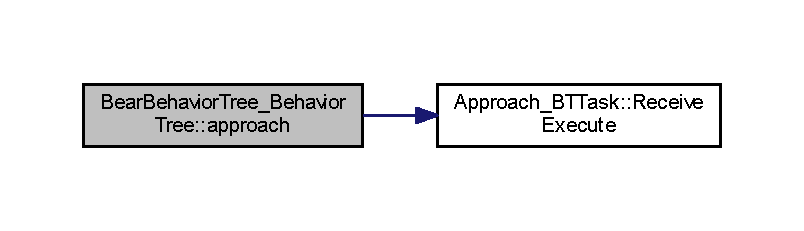
\includegraphics[width=350pt]{class_bear_behavior_tree___behavior_tree_ae22286b24ddb389f5c147fca13aac2b4_cgraph}
\end{center}
\end{figure}




Here is the caller graph for this function\+:\nopagebreak
\begin{figure}[H]
\begin{center}
\leavevmode
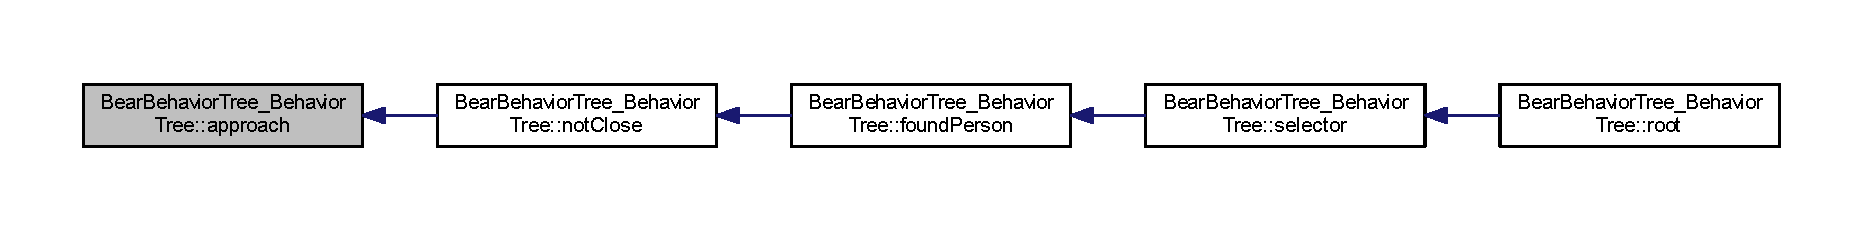
\includegraphics[width=350pt]{class_bear_behavior_tree___behavior_tree_ae22286b24ddb389f5c147fca13aac2b4_icgraph}
\end{center}
\end{figure}


\index{Bear\+Behavior\+Tree\+\_\+\+Behavior\+Tree@{Bear\+Behavior\+Tree\+\_\+\+Behavior\+Tree}!attack@{attack}}
\index{attack@{attack}!Bear\+Behavior\+Tree\+\_\+\+Behavior\+Tree@{Bear\+Behavior\+Tree\+\_\+\+Behavior\+Tree}}
\subsubsection[{\texorpdfstring{attack(\+Object target\+To\+Attack)}{attack(Object targetToAttack)}}]{\setlength{\rightskip}{0pt plus 5cm}void Bear\+Behavior\+Tree\+\_\+\+Behavior\+Tree\+::attack (
\begin{DoxyParamCaption}
\item[{Object}]{target\+To\+Attack}
\end{DoxyParamCaption}
)}\hypertarget{class_bear_behavior_tree___behavior_tree_a03d8bdee8baffed5b5f51351302744da}{}\label{class_bear_behavior_tree___behavior_tree_a03d8bdee8baffed5b5f51351302744da}


공격 태스크 

대상에게 근접 공격 기능을 수행한다. 
\begin{DoxyParams}{Parameters}
{\em target\+To\+Attack} & 공격할 대상. \\
\hline
\end{DoxyParams}


Here is the call graph for this function\+:\nopagebreak
\begin{figure}[H]
\begin{center}
\leavevmode
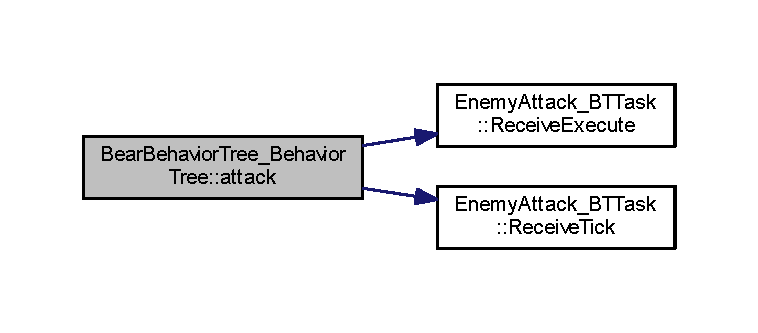
\includegraphics[width=350pt]{class_bear_behavior_tree___behavior_tree_a03d8bdee8baffed5b5f51351302744da_cgraph}
\end{center}
\end{figure}




Here is the caller graph for this function\+:\nopagebreak
\begin{figure}[H]
\begin{center}
\leavevmode
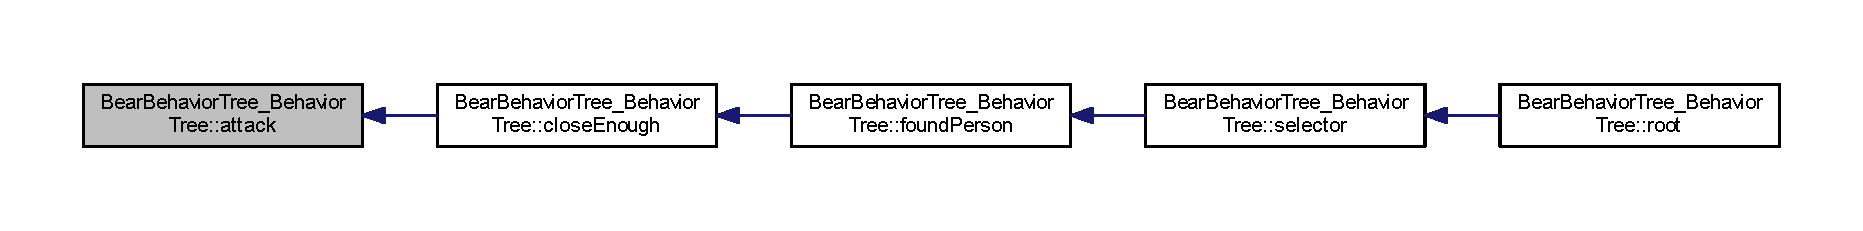
\includegraphics[width=350pt]{class_bear_behavior_tree___behavior_tree_a03d8bdee8baffed5b5f51351302744da_icgraph}
\end{center}
\end{figure}


\index{Bear\+Behavior\+Tree\+\_\+\+Behavior\+Tree@{Bear\+Behavior\+Tree\+\_\+\+Behavior\+Tree}!close\+Enough@{close\+Enough}}
\index{close\+Enough@{close\+Enough}!Bear\+Behavior\+Tree\+\_\+\+Behavior\+Tree@{Bear\+Behavior\+Tree\+\_\+\+Behavior\+Tree}}
\subsubsection[{\texorpdfstring{close\+Enough(\+Object target\+To\+Attack)}{closeEnough(Object targetToAttack)}}]{\setlength{\rightskip}{0pt plus 5cm}void Bear\+Behavior\+Tree\+\_\+\+Behavior\+Tree\+::close\+Enough (
\begin{DoxyParamCaption}
\item[{Object}]{target\+To\+Attack}
\end{DoxyParamCaption}
)}\hypertarget{class_bear_behavior_tree___behavior_tree_a1277dd95b086e24e0babaccff90a7609}{}\label{class_bear_behavior_tree___behavior_tree_a1277dd95b086e24e0babaccff90a7609}


근접 상태 데코레이터 

적을 근접 공격할 수 있을 정도로 충분히 가까우면 attack을 호출한다. 
\begin{DoxyParams}{Parameters}
{\em target\+To\+Attack} & 공격할 대상. \\
\hline
\end{DoxyParams}


Here is the call graph for this function\+:\nopagebreak
\begin{figure}[H]
\begin{center}
\leavevmode
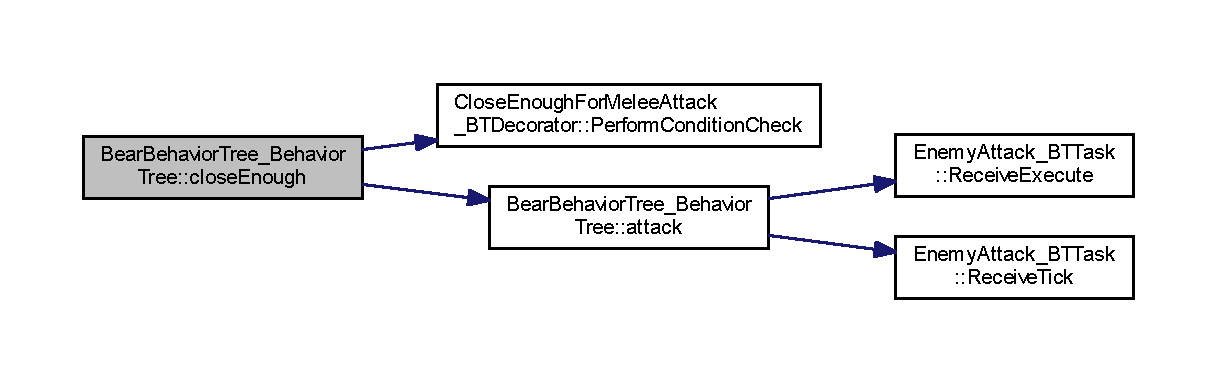
\includegraphics[width=350pt]{class_bear_behavior_tree___behavior_tree_a1277dd95b086e24e0babaccff90a7609_cgraph}
\end{center}
\end{figure}




Here is the caller graph for this function\+:\nopagebreak
\begin{figure}[H]
\begin{center}
\leavevmode
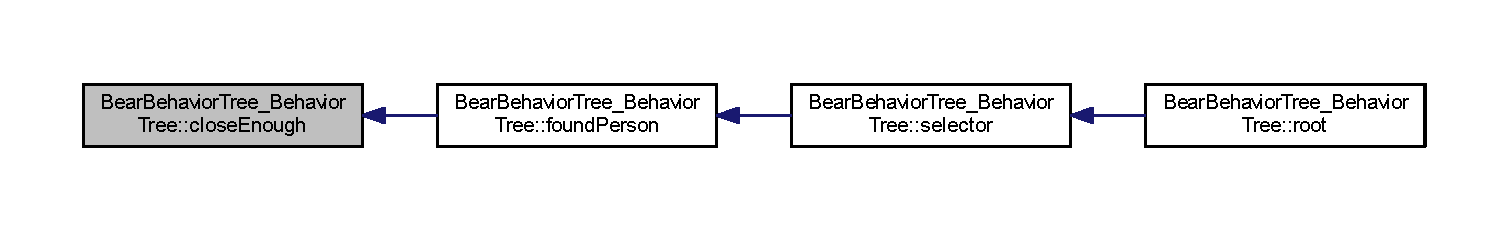
\includegraphics[width=350pt]{class_bear_behavior_tree___behavior_tree_a1277dd95b086e24e0babaccff90a7609_icgraph}
\end{center}
\end{figure}


\index{Bear\+Behavior\+Tree\+\_\+\+Behavior\+Tree@{Bear\+Behavior\+Tree\+\_\+\+Behavior\+Tree}!found\+Person@{found\+Person}}
\index{found\+Person@{found\+Person}!Bear\+Behavior\+Tree\+\_\+\+Behavior\+Tree@{Bear\+Behavior\+Tree\+\_\+\+Behavior\+Tree}}
\subsubsection[{\texorpdfstring{found\+Person(\+Object target\+To\+Attack)}{foundPerson(Object targetToAttack)}}]{\setlength{\rightskip}{0pt plus 5cm}void Bear\+Behavior\+Tree\+\_\+\+Behavior\+Tree\+::found\+Person (
\begin{DoxyParamCaption}
\item[{Object}]{target\+To\+Attack}
\end{DoxyParamCaption}
)}\hypertarget{class_bear_behavior_tree___behavior_tree_a13134307abf8a5c1f0edef371b78f40b}{}\label{class_bear_behavior_tree___behavior_tree_a13134307abf8a5c1f0edef371b78f40b}


전투 상태 데코레이터 

target\+To\+Attack에 값이 있으면 이쪽으로 분기된다. 
\begin{DoxyParams}{Parameters}
{\em target\+To\+Attack} & 공격할 대상. \\
\hline
\end{DoxyParams}


Here is the call graph for this function\+:\nopagebreak
\begin{figure}[H]
\begin{center}
\leavevmode
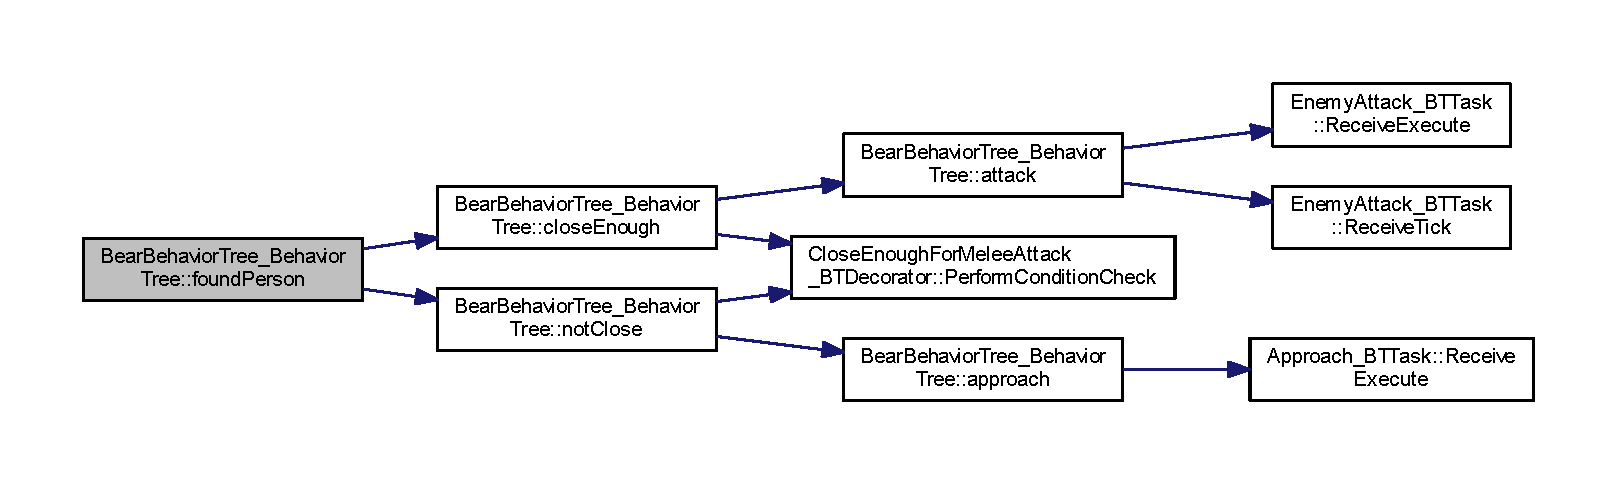
\includegraphics[width=350pt]{class_bear_behavior_tree___behavior_tree_a13134307abf8a5c1f0edef371b78f40b_cgraph}
\end{center}
\end{figure}




Here is the caller graph for this function\+:\nopagebreak
\begin{figure}[H]
\begin{center}
\leavevmode
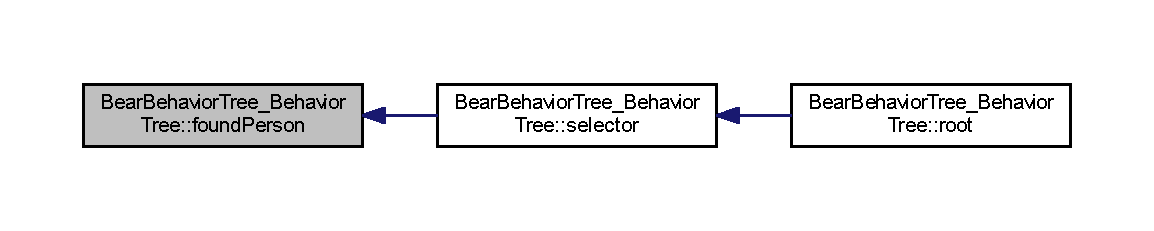
\includegraphics[width=350pt]{class_bear_behavior_tree___behavior_tree_a13134307abf8a5c1f0edef371b78f40b_icgraph}
\end{center}
\end{figure}


\index{Bear\+Behavior\+Tree\+\_\+\+Behavior\+Tree@{Bear\+Behavior\+Tree\+\_\+\+Behavior\+Tree}!idle@{idle}}
\index{idle@{idle}!Bear\+Behavior\+Tree\+\_\+\+Behavior\+Tree@{Bear\+Behavior\+Tree\+\_\+\+Behavior\+Tree}}
\subsubsection[{\texorpdfstring{idle(\+Object target\+To\+Attack)}{idle(Object targetToAttack)}}]{\setlength{\rightskip}{0pt plus 5cm}void Bear\+Behavior\+Tree\+\_\+\+Behavior\+Tree\+::idle (
\begin{DoxyParamCaption}
\item[{Object}]{target\+To\+Attack}
\end{DoxyParamCaption}
)}\hypertarget{class_bear_behavior_tree___behavior_tree_af17627dd1013988585a7afec3e36b00b}{}\label{class_bear_behavior_tree___behavior_tree_af17627dd1013988585a7afec3e36b00b}


대기 상태 데코레이터 

target\+To\+Attack이 비어있을 경우 이쪽으로 분기된다. 
\begin{DoxyParams}{Parameters}
{\em target\+To\+Attack} & 공격할 대상. \\
\hline
\end{DoxyParams}


Here is the call graph for this function\+:\nopagebreak
\begin{figure}[H]
\begin{center}
\leavevmode
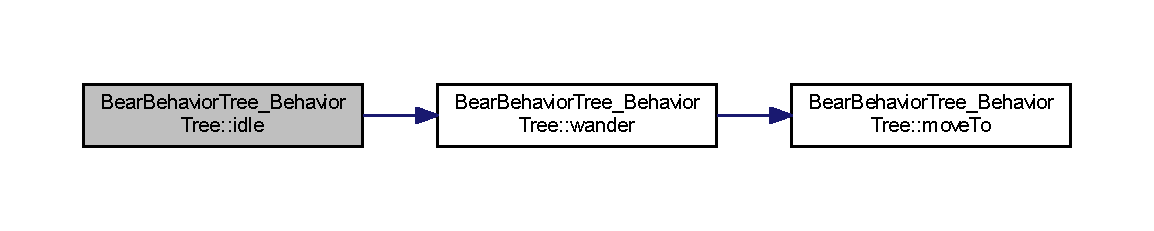
\includegraphics[width=350pt]{class_bear_behavior_tree___behavior_tree_af17627dd1013988585a7afec3e36b00b_cgraph}
\end{center}
\end{figure}




Here is the caller graph for this function\+:\nopagebreak
\begin{figure}[H]
\begin{center}
\leavevmode
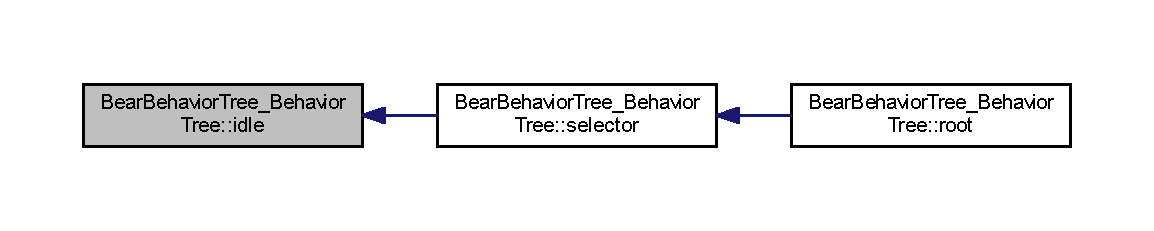
\includegraphics[width=350pt]{class_bear_behavior_tree___behavior_tree_af17627dd1013988585a7afec3e36b00b_icgraph}
\end{center}
\end{figure}


\index{Bear\+Behavior\+Tree\+\_\+\+Behavior\+Tree@{Bear\+Behavior\+Tree\+\_\+\+Behavior\+Tree}!move\+To@{move\+To}}
\index{move\+To@{move\+To}!Bear\+Behavior\+Tree\+\_\+\+Behavior\+Tree@{Bear\+Behavior\+Tree\+\_\+\+Behavior\+Tree}}
\subsubsection[{\texorpdfstring{move\+To(\+Vector destination)}{moveTo(Vector destination)}}]{\setlength{\rightskip}{0pt plus 5cm}void Bear\+Behavior\+Tree\+\_\+\+Behavior\+Tree\+::move\+To (
\begin{DoxyParamCaption}
\item[{Vector}]{destination}
\end{DoxyParamCaption}
)}\hypertarget{class_bear_behavior_tree___behavior_tree_aba205bd3c0ead482d7dff54693a7b2a2}{}\label{class_bear_behavior_tree___behavior_tree_aba205bd3c0ead482d7dff54693a7b2a2}


이동 태스크 

언리얼에서 제공하는 기본 이동 태스크. 
\begin{DoxyParams}{Parameters}
{\em destination} & 이동할 목적지. \\
\hline
\end{DoxyParams}


Here is the caller graph for this function\+:\nopagebreak
\begin{figure}[H]
\begin{center}
\leavevmode
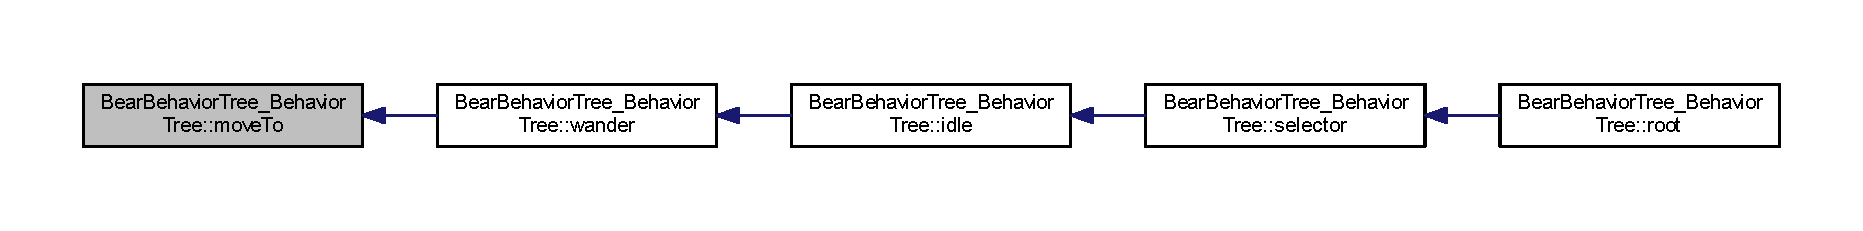
\includegraphics[width=350pt]{class_bear_behavior_tree___behavior_tree_aba205bd3c0ead482d7dff54693a7b2a2_icgraph}
\end{center}
\end{figure}


\index{Bear\+Behavior\+Tree\+\_\+\+Behavior\+Tree@{Bear\+Behavior\+Tree\+\_\+\+Behavior\+Tree}!not\+Close@{not\+Close}}
\index{not\+Close@{not\+Close}!Bear\+Behavior\+Tree\+\_\+\+Behavior\+Tree@{Bear\+Behavior\+Tree\+\_\+\+Behavior\+Tree}}
\subsubsection[{\texorpdfstring{not\+Close(\+Object target\+To\+Attack)}{notClose(Object targetToAttack)}}]{\setlength{\rightskip}{0pt plus 5cm}void Bear\+Behavior\+Tree\+\_\+\+Behavior\+Tree\+::not\+Close (
\begin{DoxyParamCaption}
\item[{Object}]{target\+To\+Attack}
\end{DoxyParamCaption}
)}\hypertarget{class_bear_behavior_tree___behavior_tree_a4fb3030436667eba76f35eff2201b13b}{}\label{class_bear_behavior_tree___behavior_tree_a4fb3030436667eba76f35eff2201b13b}


멀리 떨어진 상태 데코레이터 

적을 근접 공격할 수 있을 정도로 가깝지 않으면 approach를 호출한다. 
\begin{DoxyParams}{Parameters}
{\em target\+To\+Attack} & 공격할 대상. \\
\hline
\end{DoxyParams}


Here is the call graph for this function\+:\nopagebreak
\begin{figure}[H]
\begin{center}
\leavevmode
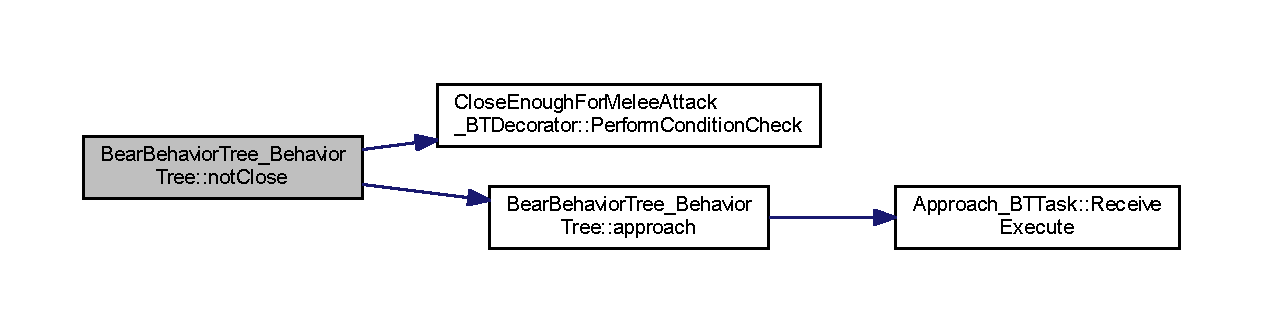
\includegraphics[width=350pt]{class_bear_behavior_tree___behavior_tree_a4fb3030436667eba76f35eff2201b13b_cgraph}
\end{center}
\end{figure}




Here is the caller graph for this function\+:\nopagebreak
\begin{figure}[H]
\begin{center}
\leavevmode
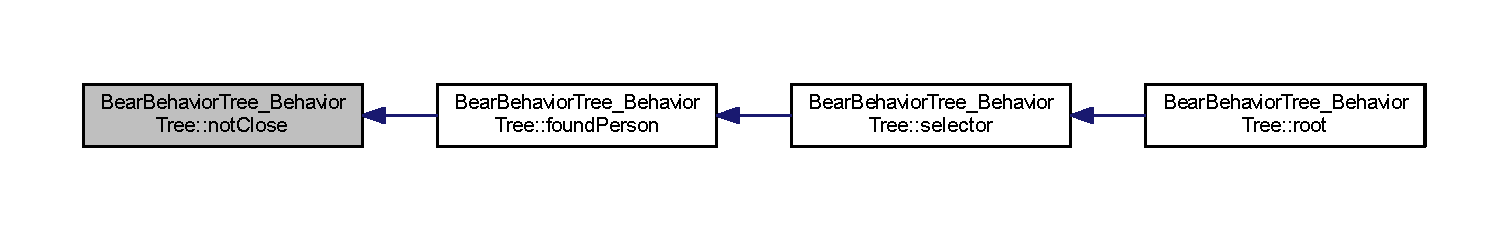
\includegraphics[width=350pt]{class_bear_behavior_tree___behavior_tree_a4fb3030436667eba76f35eff2201b13b_icgraph}
\end{center}
\end{figure}


\index{Bear\+Behavior\+Tree\+\_\+\+Behavior\+Tree@{Bear\+Behavior\+Tree\+\_\+\+Behavior\+Tree}!root@{root}}
\index{root@{root}!Bear\+Behavior\+Tree\+\_\+\+Behavior\+Tree@{Bear\+Behavior\+Tree\+\_\+\+Behavior\+Tree}}
\subsubsection[{\texorpdfstring{root(\+Enemy\+Blackboard\+\_\+\+Blackboard blackboard)}{root(EnemyBlackboard_Blackboard blackboard)}}]{\setlength{\rightskip}{0pt plus 5cm}void Bear\+Behavior\+Tree\+\_\+\+Behavior\+Tree\+::root (
\begin{DoxyParamCaption}
\item[{{\bf Enemy\+Blackboard\+\_\+\+Blackboard}}]{blackboard}
\end{DoxyParamCaption}
)}\hypertarget{class_bear_behavior_tree___behavior_tree_a67e899c19fdc37eb5ed077d882ae4ad1}{}\label{class_bear_behavior_tree___behavior_tree_a67e899c19fdc37eb5ed077d882ae4ad1}


루트 노드 

비헤이비어 트리의 루트 노드. 
\begin{DoxyParams}{Parameters}
{\em blackboard} & 비헤이비어 트리에서 사용하는 블랙보드. \\
\hline
\end{DoxyParams}


Here is the call graph for this function\+:\nopagebreak
\begin{figure}[H]
\begin{center}
\leavevmode
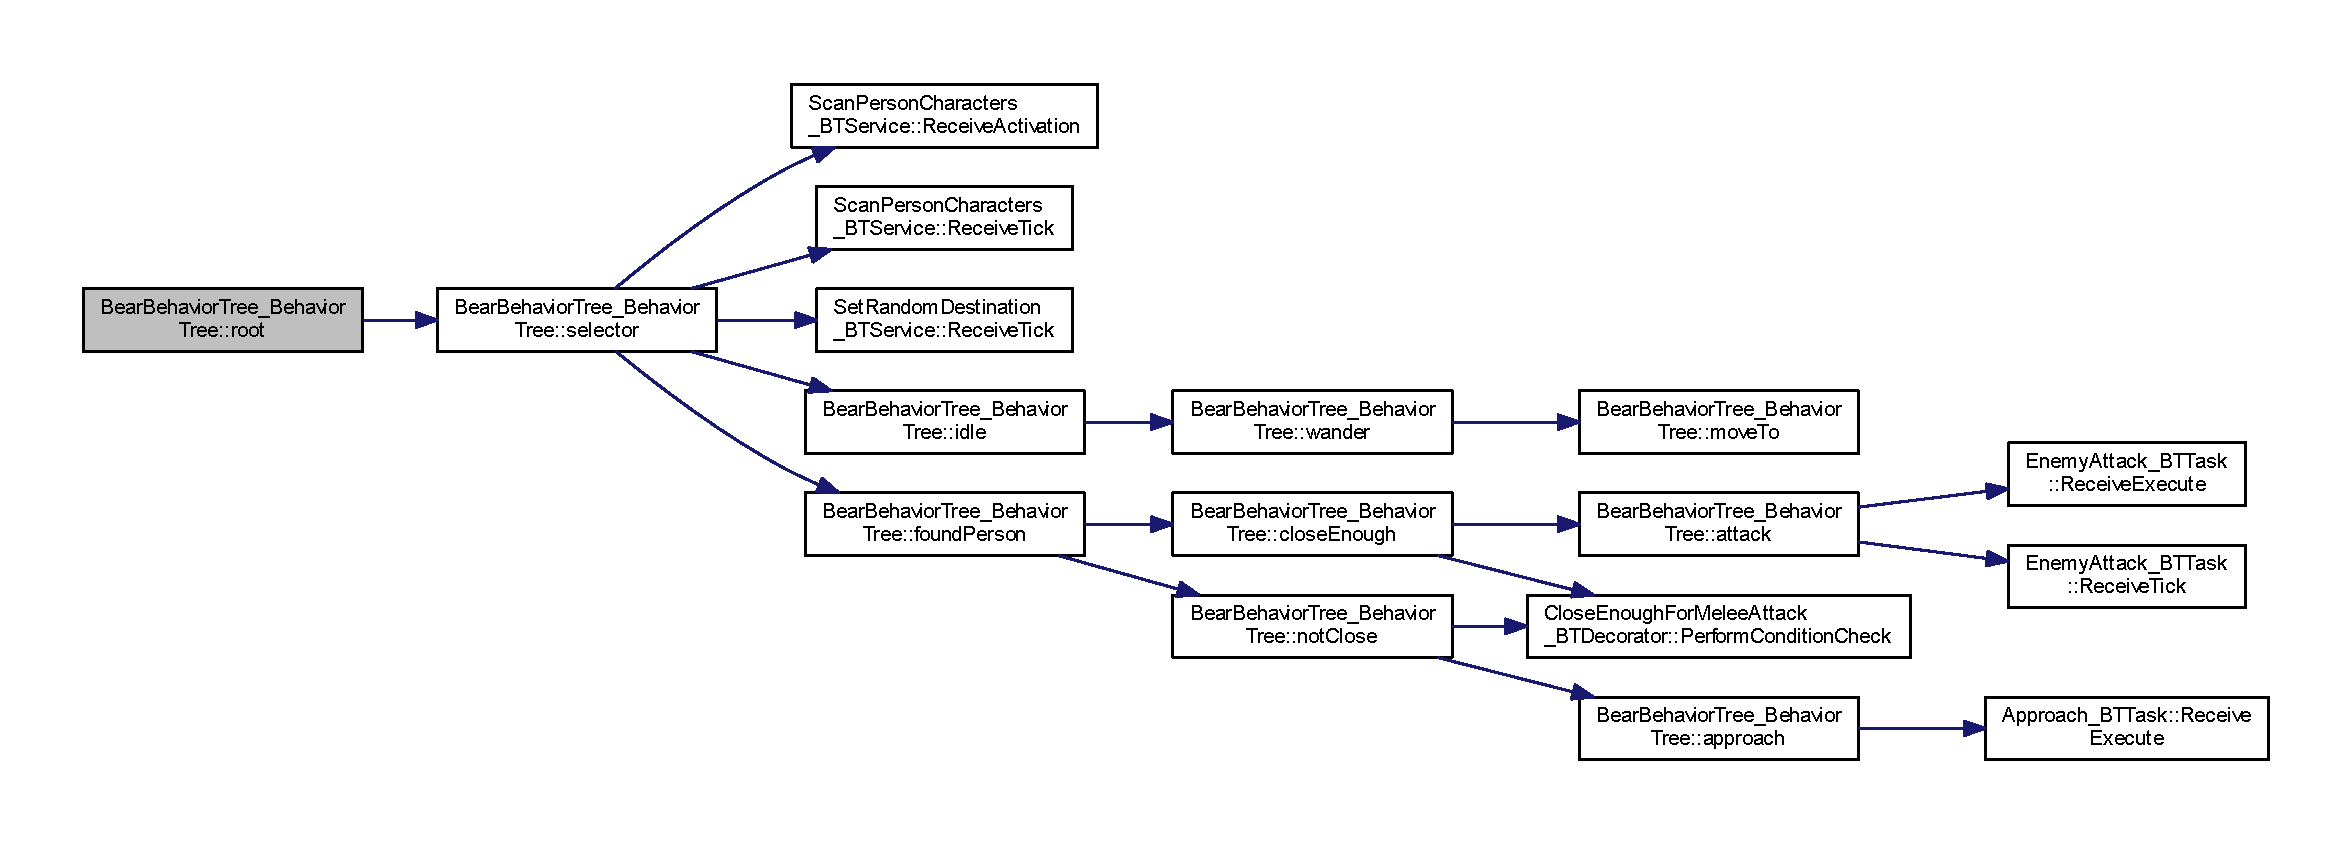
\includegraphics[width=350pt]{class_bear_behavior_tree___behavior_tree_a67e899c19fdc37eb5ed077d882ae4ad1_cgraph}
\end{center}
\end{figure}


\index{Bear\+Behavior\+Tree\+\_\+\+Behavior\+Tree@{Bear\+Behavior\+Tree\+\_\+\+Behavior\+Tree}!selector@{selector}}
\index{selector@{selector}!Bear\+Behavior\+Tree\+\_\+\+Behavior\+Tree@{Bear\+Behavior\+Tree\+\_\+\+Behavior\+Tree}}
\subsubsection[{\texorpdfstring{selector(\+Object target\+To\+Attack, Vector destination)}{selector(Object targetToAttack, Vector destination)}}]{\setlength{\rightskip}{0pt plus 5cm}void Bear\+Behavior\+Tree\+\_\+\+Behavior\+Tree\+::selector (
\begin{DoxyParamCaption}
\item[{Object}]{target\+To\+Attack, }
\item[{Vector}]{destination}
\end{DoxyParamCaption}
)}\hypertarget{class_bear_behavior_tree___behavior_tree_a1d4c26a6c9f2c056a5d07f956129ba19}{}\label{class_bear_behavior_tree___behavior_tree_a1d4c26a6c9f2c056a5d07f956129ba19}


서비스를 가지는 분기 노드 

Scan\+Person\+Character와 Set\+Random\+Destination 서비스를 가지고 있다. 
\begin{DoxyParams}{Parameters}
{\em target\+To\+Attack} & 인간 캐릭터를 발견하면 이 변수에 저장된다. \\
\hline
{\em destination} & 주위 -\/2000 $\sim$ +2000 범위의 랜덤 위치가 저장된다. \\
\hline
\end{DoxyParams}


Here is the call graph for this function\+:\nopagebreak
\begin{figure}[H]
\begin{center}
\leavevmode
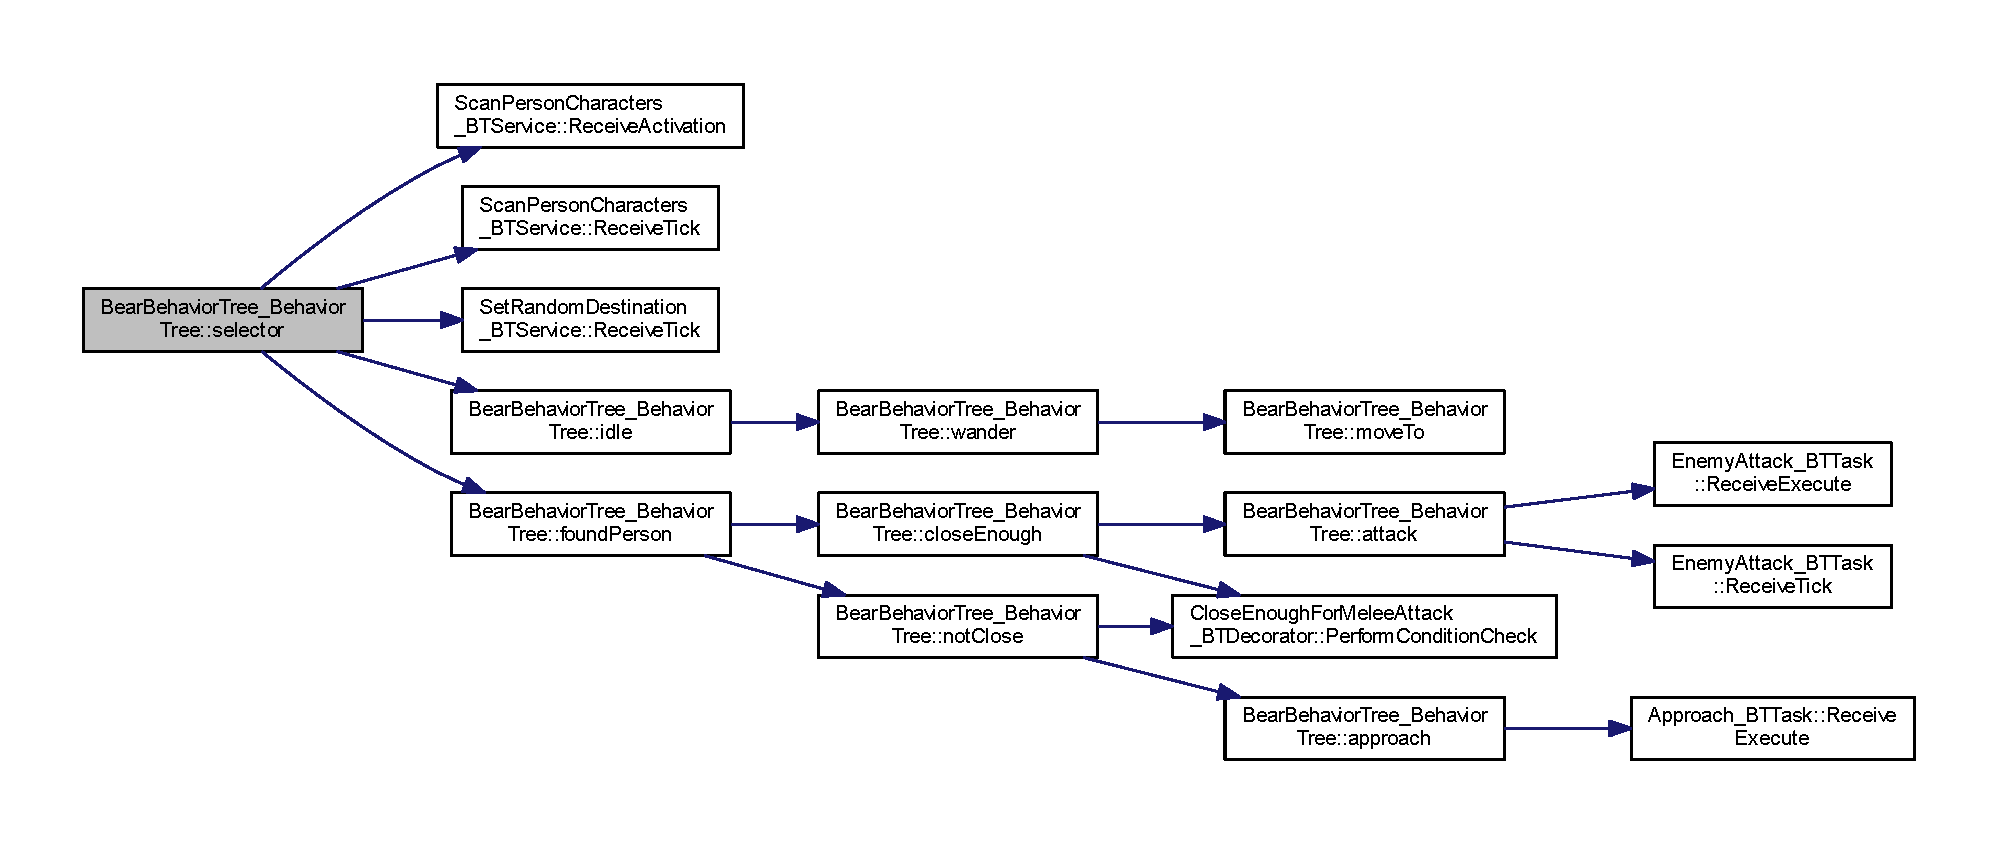
\includegraphics[width=350pt]{class_bear_behavior_tree___behavior_tree_a1d4c26a6c9f2c056a5d07f956129ba19_cgraph}
\end{center}
\end{figure}




Here is the caller graph for this function\+:\nopagebreak
\begin{figure}[H]
\begin{center}
\leavevmode
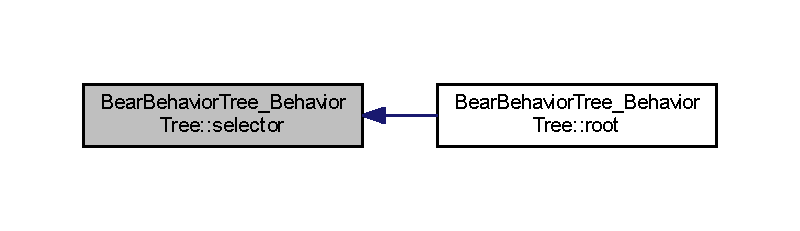
\includegraphics[width=350pt]{class_bear_behavior_tree___behavior_tree_a1d4c26a6c9f2c056a5d07f956129ba19_icgraph}
\end{center}
\end{figure}


\index{Bear\+Behavior\+Tree\+\_\+\+Behavior\+Tree@{Bear\+Behavior\+Tree\+\_\+\+Behavior\+Tree}!wander@{wander}}
\index{wander@{wander}!Bear\+Behavior\+Tree\+\_\+\+Behavior\+Tree@{Bear\+Behavior\+Tree\+\_\+\+Behavior\+Tree}}
\subsubsection[{\texorpdfstring{wander(\+Vector destination)}{wander(Vector destination)}}]{\setlength{\rightskip}{0pt plus 5cm}void Bear\+Behavior\+Tree\+\_\+\+Behavior\+Tree\+::wander (
\begin{DoxyParamCaption}
\item[{Vector}]{destination}
\end{DoxyParamCaption}
)}\hypertarget{class_bear_behavior_tree___behavior_tree_a0dcee292ae4de16888b71b3eafcfa6a9}{}\label{class_bear_behavior_tree___behavior_tree_a0dcee292ae4de16888b71b3eafcfa6a9}


어슬렁거리기 데코레이터 

공격할 대상이 없고 destination에 값이 있으면 move\+To를 호출한다. 
\begin{DoxyParams}{Parameters}
{\em destination} & 이동할 목적지. \\
\hline
\end{DoxyParams}


Here is the call graph for this function\+:\nopagebreak
\begin{figure}[H]
\begin{center}
\leavevmode
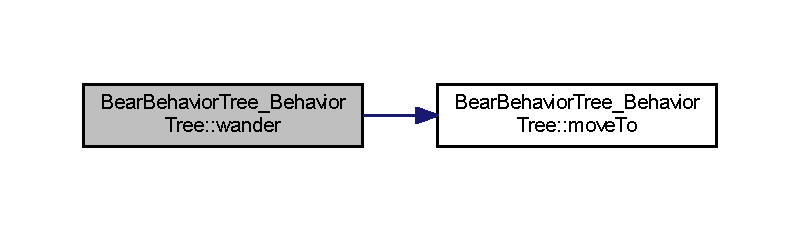
\includegraphics[width=350pt]{class_bear_behavior_tree___behavior_tree_a0dcee292ae4de16888b71b3eafcfa6a9_cgraph}
\end{center}
\end{figure}




Here is the caller graph for this function\+:\nopagebreak
\begin{figure}[H]
\begin{center}
\leavevmode
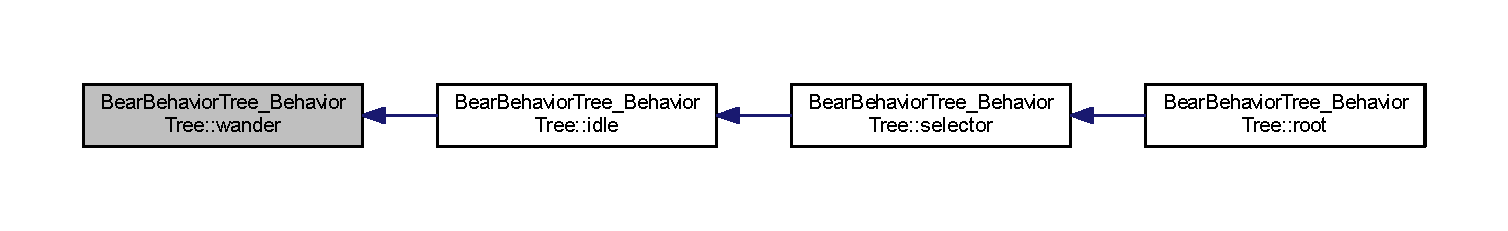
\includegraphics[width=350pt]{class_bear_behavior_tree___behavior_tree_a0dcee292ae4de16888b71b3eafcfa6a9_icgraph}
\end{center}
\end{figure}




\subsection{Member Data Documentation}
\index{Bear\+Behavior\+Tree\+\_\+\+Behavior\+Tree@{Bear\+Behavior\+Tree\+\_\+\+Behavior\+Tree}!blackboard@{blackboard}}
\index{blackboard@{blackboard}!Bear\+Behavior\+Tree\+\_\+\+Behavior\+Tree@{Bear\+Behavior\+Tree\+\_\+\+Behavior\+Tree}}
\subsubsection[{\texorpdfstring{blackboard}{blackboard}}]{\setlength{\rightskip}{0pt plus 5cm}{\bf Enemy\+Blackboard\+\_\+\+Blackboard} Bear\+Behavior\+Tree\+\_\+\+Behavior\+Tree\+::blackboard\hspace{0.3cm}{\ttfamily [private]}}\hypertarget{class_bear_behavior_tree___behavior_tree_af65805184758188534eb2100723629d7}{}\label{class_bear_behavior_tree___behavior_tree_af65805184758188534eb2100723629d7}

\hypertarget{class_b_t___base}{}\section{B\+T\+\_\+\+Base Class Reference}
\label{class_b_t___base}\index{B\+T\+\_\+\+Base@{B\+T\+\_\+\+Base}}


팀원\+A\+I들의 기본적인 비헤이비어 트리  




{\ttfamily \#include $<$B\+T\+\_\+\+Base.\+h$>$}



Inheritance diagram for B\+T\+\_\+\+Base\+:
\nopagebreak
\begin{figure}[H]
\begin{center}
\leavevmode
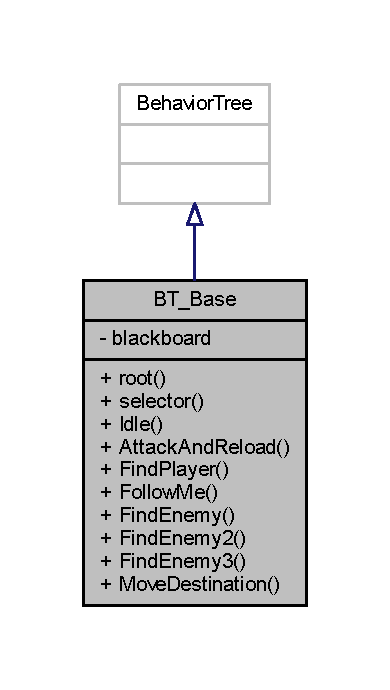
\includegraphics[width=187pt]{class_b_t___base__inherit__graph}
\end{center}
\end{figure}


Collaboration diagram for B\+T\+\_\+\+Base\+:
\nopagebreak
\begin{figure}[H]
\begin{center}
\leavevmode
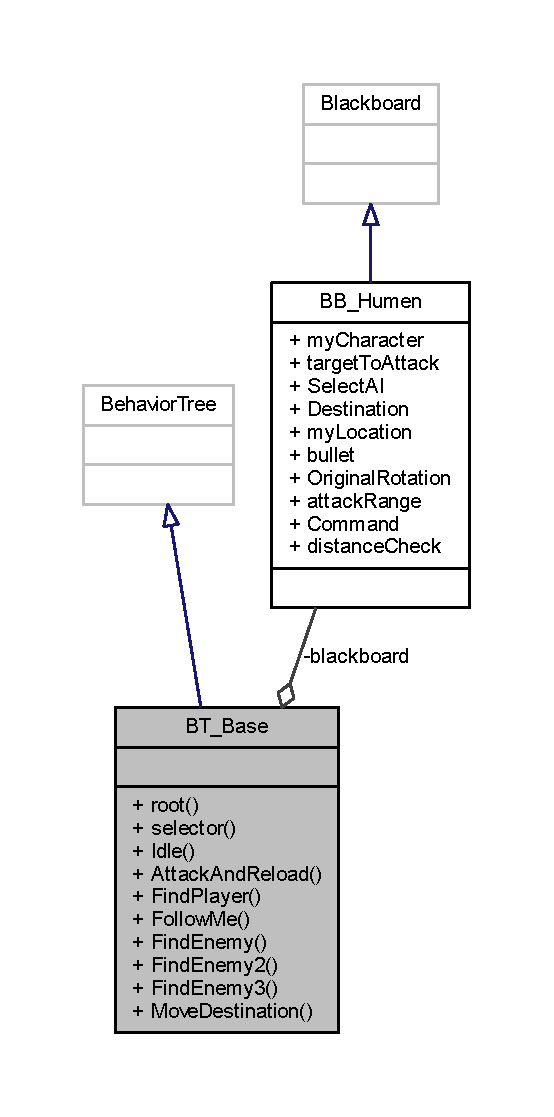
\includegraphics[width=320pt]{class_b_t___base__coll__graph}
\end{center}
\end{figure}
\subsection*{Public Member Functions}
\begin{DoxyCompactItemize}
\item 
void \hyperlink{class_b_t___base_a54881cf55e411fdbf6c9f98586049742}{root} (\hyperlink{class_b_b___humen}{B\+B\+\_\+\+Humen} \hyperlink{class_b_t___base_a8a095b67df2778f5155d24dad9f818ef}{blackboard})
\begin{DoxyCompactList}\small\item\em 루트 노드 \end{DoxyCompactList}\item 
void \hyperlink{class_b_t___base_adbbf3731340b4e525a1ea549fd6409f3}{selector} (Object my\+Character, Vector my\+Location, Vector Destination, Bool distance\+Check, Object target\+To\+Attack, Float attack\+Range, Integer bullet, Object Select\+AI, Bool Command, Rotator Original\+Rotation)
\begin{DoxyCompactList}\small\item\em 서비스를 가지는 분기 노드 \end{DoxyCompactList}\item 
void \hyperlink{class_b_t___base_a68cb1b35bc3105c36e0bd4b8477a1ec9}{Idle} (Bool Command)
\begin{DoxyCompactList}\small\item\em 대기 상태 데코레이터 \end{DoxyCompactList}\item 
void \hyperlink{class_b_t___base_affb0d6cdaec417994ce78c7608e5bf9e}{Find} (Object target\+To\+Attack, Integer bullet, Bool \hyperlink{class_dec___player_check}{Dec\+\_\+\+Player\+Check})
\begin{DoxyCompactList}\small\item\em 적 발견 상태 데코레이터 \end{DoxyCompactList}\item 
void \hyperlink{class_b_t___base_a4473d81f72741d7b1b4956feada36a28}{Attack\+And\+Reload} (Object target\+To\+Attack, Integer bullet)
\begin{DoxyCompactList}\small\item\em 적을 공격하는 태스크 \end{DoxyCompactList}\item 
void \hyperlink{class_b_t___base_a185c89f6b41c5946e6dac9489f251c0f}{Find\+Player} (Bool Command, Object my\+Character, Rotator Original\+Rotation)
\begin{DoxyCompactList}\small\item\em 플레이어가 범위에 있는지 확인하는 데코레이터 \end{DoxyCompactList}\item 
void \hyperlink{class_b_t___base_a802b9e457808b511a6bc5ea63abd3b87}{Follow\+Me} (Bool Command, Vector Destination, Vector my\+Location, Bool distance\+Check)
\begin{DoxyCompactList}\small\item\em 나를 따라오게 하는 태스크 \end{DoxyCompactList}\item 
void \hyperlink{class_b_t___base_aae303238f1a4876a0dc077a91c25b57f}{Find\+Enemy} (Object my\+Characyer, Bool Command, Object target\+To\+Attack)
\begin{DoxyCompactList}\small\item\em 적이 범위에 있는지 확인하는 데코레이터 \end{DoxyCompactList}\item 
void \hyperlink{class_b_t___base_a589c2fe0cc37e24c84ea3ed57157dc60}{Move\+Destination} (Bool Command, Vector Destination, Vector, my\+Location, Bool distance\+Check)
\begin{DoxyCompactList}\small\item\em 명령을 받아서 목적지로 이동하는 태스크 \end{DoxyCompactList}\end{DoxyCompactItemize}
\subsection*{Private Attributes}
\begin{DoxyCompactItemize}
\item 
\hyperlink{class_enemy_blackboard___blackboard}{Enemy\+Blackboard\+\_\+\+Blackboard} \hyperlink{class_b_t___base_a8a095b67df2778f5155d24dad9f818ef}{blackboard}
\end{DoxyCompactItemize}


\subsection{Detailed Description}
팀원\+A\+I들의 기본적인 비헤이비어 트리 

모든 팀원들의 행동 방식을 컨트롤 한다. 

\subsection{Member Function Documentation}
\index{B\+T\+\_\+\+Base@{B\+T\+\_\+\+Base}!Attack\+And\+Reload@{Attack\+And\+Reload}}
\index{Attack\+And\+Reload@{Attack\+And\+Reload}!B\+T\+\_\+\+Base@{B\+T\+\_\+\+Base}}
\subsubsection[{\texorpdfstring{Attack\+And\+Reload(\+Object target\+To\+Attack, Integer bullet)}{AttackAndReload(Object targetToAttack, Integer bullet)}}]{\setlength{\rightskip}{0pt plus 5cm}void B\+T\+\_\+\+Base\+::\+Attack\+And\+Reload (
\begin{DoxyParamCaption}
\item[{Object}]{target\+To\+Attack, }
\item[{Integer}]{bullet}
\end{DoxyParamCaption}
)}\hypertarget{class_b_t___base_a4473d81f72741d7b1b4956feada36a28}{}\label{class_b_t___base_a4473d81f72741d7b1b4956feada36a28}


적을 공격하는 태스크 

Find에 의해 Attack\+And\+Reload가 실행되면 설정된 target\+To\+Attack의 위치로 공격을 시작함. 
\begin{DoxyParams}{Parameters}
{\em target\+To\+Attack은} & 공격할 대상. \\
\hline
{\em bullet은} & 현재 총알이 장전된 수 \\
\hline
\end{DoxyParams}
\index{B\+T\+\_\+\+Base@{B\+T\+\_\+\+Base}!Find@{Find}}
\index{Find@{Find}!B\+T\+\_\+\+Base@{B\+T\+\_\+\+Base}}
\subsubsection[{\texorpdfstring{Find(\+Object target\+To\+Attack, Integer bullet, Bool Dec\+\_\+\+Player\+Check)}{Find(Object targetToAttack, Integer bullet, Bool Dec_PlayerCheck)}}]{\setlength{\rightskip}{0pt plus 5cm}void B\+T\+\_\+\+Base\+::\+Find (
\begin{DoxyParamCaption}
\item[{Object}]{target\+To\+Attack, }
\item[{Integer}]{bullet, }
\item[{Bool}]{Dec\+\_\+\+Player\+Check}
\end{DoxyParamCaption}
)}\hypertarget{class_b_t___base_affb0d6cdaec417994ce78c7608e5bf9e}{}\label{class_b_t___base_affb0d6cdaec417994ce78c7608e5bf9e}


적 발견 상태 데코레이터 

Idle에 의해 Find가 실행되면 target\+To\+Attack = true, bullet $>$ 0, 플레이어가 근처에 있다면 Attack\+And\+Reload가 실행된다. 
\begin{DoxyParams}{Parameters}
{\em target\+To\+Attack은} & 공격할 대상. \\
\hline
{\em bullet은} & 현재 총알이 장전된 수 \\
\hline
{\em Dec\+\_\+\+Player\+Check는} & 설정된 범위안에 플레이어가 있는지 체크. 해당 변수는 따로 만들어진 데코레이터 파일로 인해 반환된다. \\
\hline
\end{DoxyParams}
\index{B\+T\+\_\+\+Base@{B\+T\+\_\+\+Base}!Find\+Enemy@{Find\+Enemy}}
\index{Find\+Enemy@{Find\+Enemy}!B\+T\+\_\+\+Base@{B\+T\+\_\+\+Base}}
\subsubsection[{\texorpdfstring{Find\+Enemy(\+Object my\+Characyer, Bool Command, Object target\+To\+Attack)}{FindEnemy(Object myCharacyer, Bool Command, Object targetToAttack)}}]{\setlength{\rightskip}{0pt plus 5cm}void B\+T\+\_\+\+Base\+::\+Find\+Enemy (
\begin{DoxyParamCaption}
\item[{Object}]{my\+Characyer, }
\item[{Bool}]{Command, }
\item[{Object}]{target\+To\+Attack}
\end{DoxyParamCaption}
)}\hypertarget{class_b_t___base_aae303238f1a4876a0dc077a91c25b57f}{}\label{class_b_t___base_aae303238f1a4876a0dc077a91c25b57f}


적이 범위에 있는지 확인하는 데코레이터 

Command == True, target\+To\+Attack == False가 만족하면 my\+Character에 따라 Move\+Destination과 Attack\+And\+Reload를 실행함. 
\begin{DoxyParams}{Parameters}
{\em commnad는} & 명령을 내렸는지 확인하는 변수 \\
\hline
{\em my\+Character는} & 플레이어 Object \\
\hline
{\em target\+To\+Attack은} & 공격할 적 Object \\
\hline
\end{DoxyParams}
\index{B\+T\+\_\+\+Base@{B\+T\+\_\+\+Base}!Find\+Player@{Find\+Player}}
\index{Find\+Player@{Find\+Player}!B\+T\+\_\+\+Base@{B\+T\+\_\+\+Base}}
\subsubsection[{\texorpdfstring{Find\+Player(\+Bool Command, Object my\+Character, Rotator Original\+Rotation)}{FindPlayer(Bool Command, Object myCharacter, Rotator OriginalRotation)}}]{\setlength{\rightskip}{0pt plus 5cm}void B\+T\+\_\+\+Base\+::\+Find\+Player (
\begin{DoxyParamCaption}
\item[{Bool}]{Command, }
\item[{Object}]{my\+Character, }
\item[{Rotator}]{Original\+Rotation}
\end{DoxyParamCaption}
)}\hypertarget{class_b_t___base_a185c89f6b41c5946e6dac9489f251c0f}{}\label{class_b_t___base_a185c89f6b41c5946e6dac9489f251c0f}


플레이어가 범위에 있는지 확인하는 데코레이터 

Command == False, my\+Character == True이 만족하면 Follow\+Me를 실행함. 
\begin{DoxyParams}{Parameters}
{\em commnad는} & 명령을 내렸는지 확인하는 변수 \\
\hline
{\em my\+Character는} & 플레이어 Object \\
\hline
{\em Dec\+\_\+\+Rotaioninit가} & 추가되어 있는데, 초기 Rotation 저장을 위한 데코레이터임. (Find\+Player의 분기과정에서 아무런 영향을 주지않음.) \\
\hline
\end{DoxyParams}
\index{B\+T\+\_\+\+Base@{B\+T\+\_\+\+Base}!Follow\+Me@{Follow\+Me}}
\index{Follow\+Me@{Follow\+Me}!B\+T\+\_\+\+Base@{B\+T\+\_\+\+Base}}
\subsubsection[{\texorpdfstring{Follow\+Me(\+Bool Command, Vector Destination, Vector my\+Location, Bool distance\+Check)}{FollowMe(Bool Command, Vector Destination, Vector myLocation, Bool distanceCheck)}}]{\setlength{\rightskip}{0pt plus 5cm}void B\+T\+\_\+\+Base\+::\+Follow\+Me (
\begin{DoxyParamCaption}
\item[{Bool}]{Command, }
\item[{Vector}]{Destination, }
\item[{Vector}]{my\+Location, }
\item[{Bool}]{distance\+Check}
\end{DoxyParamCaption}
)}\hypertarget{class_b_t___base_a802b9e457808b511a6bc5ea63abd3b87}{}\label{class_b_t___base_a802b9e457808b511a6bc5ea63abd3b87}


나를 따라오게 하는 태스크 

Find\+Player가 조건을 만족한다면 나를 따라옴. 
\begin{DoxyParams}{Parameters}
{\em Command는} & 명령을 내렸는지에 따른 변수 \\
\hline
{\em Destination은} & 명령이동시 목적지의 위치 \\
\hline
{\em my\+Location은} & 현재 플레이어의 위치 \\
\hline
{\em distance\+Check는} & 플레이어와 A\+I의 거리를 체크하는 부분 \\
\hline
\end{DoxyParams}
\index{B\+T\+\_\+\+Base@{B\+T\+\_\+\+Base}!Idle@{Idle}}
\index{Idle@{Idle}!B\+T\+\_\+\+Base@{B\+T\+\_\+\+Base}}
\subsubsection[{\texorpdfstring{Idle(\+Bool Command)}{Idle(Bool Command)}}]{\setlength{\rightskip}{0pt plus 5cm}void B\+T\+\_\+\+Base\+::\+Idle (
\begin{DoxyParamCaption}
\item[{Bool}]{Command}
\end{DoxyParamCaption}
)}\hypertarget{class_b_t___base_a68cb1b35bc3105c36e0bd4b8477a1ec9}{}\label{class_b_t___base_a68cb1b35bc3105c36e0bd4b8477a1ec9}


대기 상태 데코레이터 

Command가 false라면 Find로 간다. 
\begin{DoxyParams}{Parameters}
{\em Command는} & 명령이 내려지지 않음을 체크하기 위함. \\
\hline
\end{DoxyParams}
\index{B\+T\+\_\+\+Base@{B\+T\+\_\+\+Base}!Move\+Destination@{Move\+Destination}}
\index{Move\+Destination@{Move\+Destination}!B\+T\+\_\+\+Base@{B\+T\+\_\+\+Base}}
\subsubsection[{\texorpdfstring{Move\+Destination(\+Bool Command, Vector Destination, Vector, my\+Location, Bool distance\+Check)}{MoveDestination(Bool Command, Vector Destination, Vector, myLocation, Bool distanceCheck)}}]{\setlength{\rightskip}{0pt plus 5cm}void B\+T\+\_\+\+Base\+::\+Move\+Destination (
\begin{DoxyParamCaption}
\item[{Bool}]{Command, }
\item[{Vector}]{Destination, }
\item[{Vector}]{, }
\item[{my\+Location}]{, }
\item[{Bool}]{distance\+Check}
\end{DoxyParamCaption}
)}\hypertarget{class_b_t___base_a589c2fe0cc37e24c84ea3ed57157dc60}{}\label{class_b_t___base_a589c2fe0cc37e24c84ea3ed57157dc60}


명령을 받아서 목적지로 이동하는 태스크 

Find\+Enemy가 조건을 만족한다면 나를 따라옴. 
\begin{DoxyParams}{Parameters}
{\em Command는} & 명령을 내렸는지에 따른 변수 \\
\hline
{\em Destination은} & 명령이동시 목적지의 위치 \\
\hline
{\em my\+Location은} & 현재 플레이어의 위치 \\
\hline
{\em distance\+Check는} & 플레이어와 A\+I의 거리를 체크하는 부분 \\
\hline
\end{DoxyParams}
\index{B\+T\+\_\+\+Base@{B\+T\+\_\+\+Base}!root@{root}}
\index{root@{root}!B\+T\+\_\+\+Base@{B\+T\+\_\+\+Base}}
\subsubsection[{\texorpdfstring{root(\+B\+B\+\_\+\+Humen blackboard)}{root(BB_Humen blackboard)}}]{\setlength{\rightskip}{0pt plus 5cm}void B\+T\+\_\+\+Base\+::root (
\begin{DoxyParamCaption}
\item[{{\bf B\+B\+\_\+\+Humen}}]{blackboard}
\end{DoxyParamCaption}
)}\hypertarget{class_b_t___base_a54881cf55e411fdbf6c9f98586049742}{}\label{class_b_t___base_a54881cf55e411fdbf6c9f98586049742}


루트 노드 

비헤이비어 트리의 루트 노드. 
\begin{DoxyParams}{Parameters}
{\em blackboard} & 비헤이비어 트리에서 사용하는 블랙보드. \\
\hline
\end{DoxyParams}


Here is the call graph for this function\+:\nopagebreak
\begin{figure}[H]
\begin{center}
\leavevmode
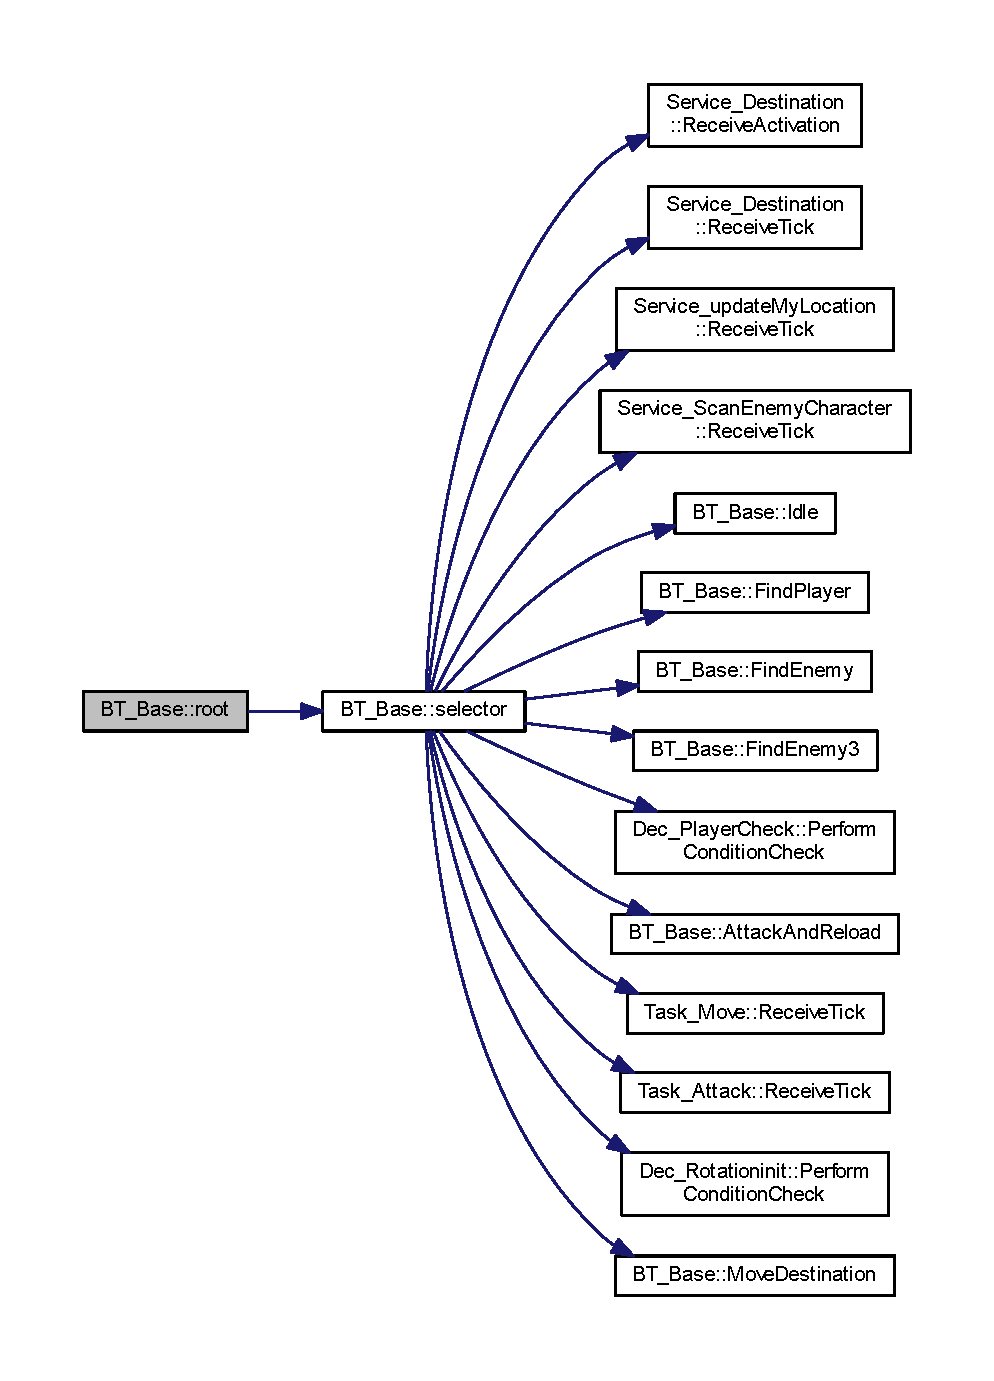
\includegraphics[width=292pt]{class_b_t___base_a54881cf55e411fdbf6c9f98586049742_cgraph}
\end{center}
\end{figure}


\index{B\+T\+\_\+\+Base@{B\+T\+\_\+\+Base}!selector@{selector}}
\index{selector@{selector}!B\+T\+\_\+\+Base@{B\+T\+\_\+\+Base}}
\subsubsection[{\texorpdfstring{selector(\+Object my\+Character, Vector my\+Location, Vector Destination, Bool distance\+Check, Object target\+To\+Attack, Float attack\+Range, Integer bullet, Object Select\+A\+I, Bool Command, Rotator Original\+Rotation)}{selector(Object myCharacter, Vector myLocation, Vector Destination, Bool distanceCheck, Object targetToAttack, Float attackRange, Integer bullet, Object SelectAI, Bool Command, Rotator OriginalRotation)}}]{\setlength{\rightskip}{0pt plus 5cm}void B\+T\+\_\+\+Base\+::selector (
\begin{DoxyParamCaption}
\item[{Object}]{my\+Character, }
\item[{Vector}]{my\+Location, }
\item[{Vector}]{Destination, }
\item[{Bool}]{distance\+Check, }
\item[{Object}]{target\+To\+Attack, }
\item[{Float}]{attack\+Range, }
\item[{Integer}]{bullet, }
\item[{Object}]{Select\+AI, }
\item[{Bool}]{Command, }
\item[{Rotator}]{Original\+Rotation}
\end{DoxyParamCaption}
)}\hypertarget{class_b_t___base_adbbf3731340b4e525a1ea549fd6409f3}{}\label{class_b_t___base_adbbf3731340b4e525a1ea549fd6409f3}


서비스를 가지는 분기 노드 

Service\+\_\+update\+My\+Locaion과 Service\+\_\+\+Scan\+Enemy\+Character, \hyperlink{class_service___destination}{Service\+\_\+\+Destination} 서비스를 가지고 있다. 
\begin{DoxyParams}{Parameters}
{\em my\+Character는} & 주변에 적이 발견된다면 on, 아니면 flase로 됨 \\
\hline
{\em my\+Location은} & 플레이어의 위치를 실시간으로 업데이트함 \\
\hline
{\em Destination은} & 명령이동시에 해당 목적지 위치를 저장한다. \\
\hline
{\em distance\+Check는} & 플레이어와 A\+I의 거리가 멀면 true, 아니면 false로 세팅된다. \\
\hline
{\em target\+To\+Attack은} & 총든 A\+I사거리에 따라 발견하는 범위안에 적이 있다면 해당 적의 Object를 세팅 \\
\hline
{\em attack\+Range는} & A\+I가 들고있는 무기를 검색해서, 무기에 따라 사거리 정해주는 초기값. \\
\hline
{\em bullet은} & 현재 장전되어 있는 탄 수를 업데이트함. \\
\hline
{\em Select\+A\+I는} & 플레이어가 팀원\+AI 중 하나를 선택하면 선택된 팀원\+A\+I의 Object를 세팅함. \\
\hline
{\em Command는} & 명령을 내렸다면 True, 아니면 False를 세팅함. \\
\hline
{\em Origina\+Rotation은} & 공격 후 이상해진 Rotation을 복구하기 위해 임시로 만든 A\+I들의 처음 Rotation 초기값. \\
\hline
\end{DoxyParams}


Here is the caller graph for this function\+:\nopagebreak
\begin{figure}[H]
\begin{center}
\leavevmode
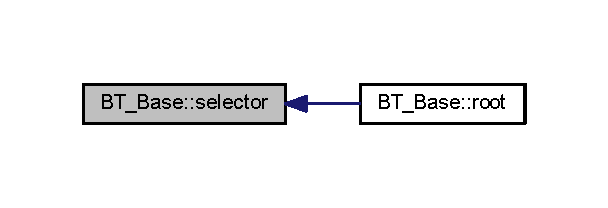
\includegraphics[width=292pt]{class_b_t___base_adbbf3731340b4e525a1ea549fd6409f3_icgraph}
\end{center}
\end{figure}




\subsection{Member Data Documentation}
\index{B\+T\+\_\+\+Base@{B\+T\+\_\+\+Base}!blackboard@{blackboard}}
\index{blackboard@{blackboard}!B\+T\+\_\+\+Base@{B\+T\+\_\+\+Base}}
\subsubsection[{\texorpdfstring{blackboard}{blackboard}}]{\setlength{\rightskip}{0pt plus 5cm}{\bf Enemy\+Blackboard\+\_\+\+Blackboard} B\+T\+\_\+\+Base\+::blackboard\hspace{0.3cm}{\ttfamily [private]}}\hypertarget{class_b_t___base_a8a095b67df2778f5155d24dad9f818ef}{}\label{class_b_t___base_a8a095b67df2778f5155d24dad9f818ef}

\hypertarget{class_close_enough_for_melee_attack___b_t_decorator}{}\section{Close\+Enough\+For\+Melee\+Attack\+\_\+\+B\+T\+Decorator Class Reference}
\label{class_close_enough_for_melee_attack___b_t_decorator}\index{Close\+Enough\+For\+Melee\+Attack\+\_\+\+B\+T\+Decorator@{Close\+Enough\+For\+Melee\+Attack\+\_\+\+B\+T\+Decorator}}


적 AI 데코레이터  




{\ttfamily \#include $<$Close\+Enough\+For\+Melee\+Attack\+\_\+\+B\+T\+Decorator.\+h$>$}



Inheritance diagram for Close\+Enough\+For\+Melee\+Attack\+\_\+\+B\+T\+Decorator\+:
\nopagebreak
\begin{figure}[H]
\begin{center}
\leavevmode
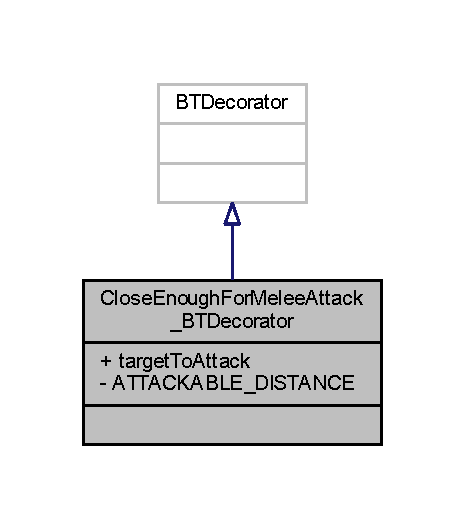
\includegraphics[width=223pt]{class_close_enough_for_melee_attack___b_t_decorator__inherit__graph}
\end{center}
\end{figure}


Collaboration diagram for Close\+Enough\+For\+Melee\+Attack\+\_\+\+B\+T\+Decorator\+:
\nopagebreak
\begin{figure}[H]
\begin{center}
\leavevmode
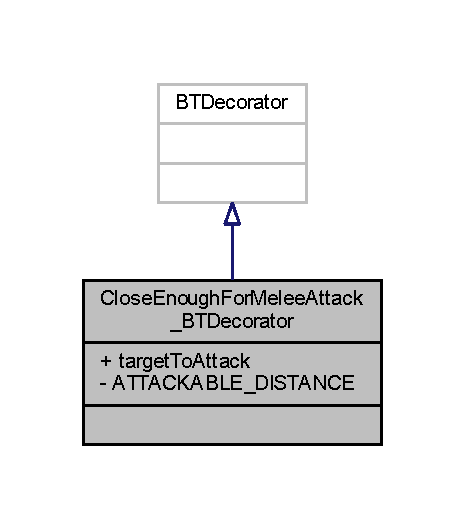
\includegraphics[width=223pt]{class_close_enough_for_melee_attack___b_t_decorator__coll__graph}
\end{center}
\end{figure}
\subsection*{Public Attributes}
\begin{DoxyCompactItemize}
\item 
Blackboard\+Key\+Selector \hyperlink{class_close_enough_for_melee_attack___b_t_decorator_a282f26ed267baec9c049ccebc61f767e}{target\+To\+Attack}
\end{DoxyCompactItemize}
\subsection*{Private Attributes}
\begin{DoxyCompactItemize}
\item 
float \hyperlink{class_close_enough_for_melee_attack___b_t_decorator_ad97a0c9cac18c905a4ae4cfe59c07815}{A\+T\+T\+A\+C\+K\+A\+B\+L\+E\+\_\+\+D\+I\+S\+T\+A\+N\+CE}
\end{DoxyCompactItemize}


\subsection{Detailed Description}
적 AI 데코레이터 

근접 공격을 할 수 있는지 판단하기 위해 공격 대상과의 거리를 검사한다. 

\subsection{Member Data Documentation}
\index{Close\+Enough\+For\+Melee\+Attack\+\_\+\+B\+T\+Decorator@{Close\+Enough\+For\+Melee\+Attack\+\_\+\+B\+T\+Decorator}!A\+T\+T\+A\+C\+K\+A\+B\+L\+E\+\_\+\+D\+I\+S\+T\+A\+N\+CE@{A\+T\+T\+A\+C\+K\+A\+B\+L\+E\+\_\+\+D\+I\+S\+T\+A\+N\+CE}}
\index{A\+T\+T\+A\+C\+K\+A\+B\+L\+E\+\_\+\+D\+I\+S\+T\+A\+N\+CE@{A\+T\+T\+A\+C\+K\+A\+B\+L\+E\+\_\+\+D\+I\+S\+T\+A\+N\+CE}!Close\+Enough\+For\+Melee\+Attack\+\_\+\+B\+T\+Decorator@{Close\+Enough\+For\+Melee\+Attack\+\_\+\+B\+T\+Decorator}}
\subsubsection[{\texorpdfstring{A\+T\+T\+A\+C\+K\+A\+B\+L\+E\+\_\+\+D\+I\+S\+T\+A\+N\+CE}{ATTACKABLE_DISTANCE}}]{\setlength{\rightskip}{0pt plus 5cm}float Close\+Enough\+For\+Melee\+Attack\+\_\+\+B\+T\+Decorator\+::\+A\+T\+T\+A\+C\+K\+A\+B\+L\+E\+\_\+\+D\+I\+S\+T\+A\+N\+CE\hspace{0.3cm}{\ttfamily [private]}}\hypertarget{class_close_enough_for_melee_attack___b_t_decorator_ad97a0c9cac18c905a4ae4cfe59c07815}{}\label{class_close_enough_for_melee_attack___b_t_decorator_ad97a0c9cac18c905a4ae4cfe59c07815}
\index{Close\+Enough\+For\+Melee\+Attack\+\_\+\+B\+T\+Decorator@{Close\+Enough\+For\+Melee\+Attack\+\_\+\+B\+T\+Decorator}!target\+To\+Attack@{target\+To\+Attack}}
\index{target\+To\+Attack@{target\+To\+Attack}!Close\+Enough\+For\+Melee\+Attack\+\_\+\+B\+T\+Decorator@{Close\+Enough\+For\+Melee\+Attack\+\_\+\+B\+T\+Decorator}}
\subsubsection[{\texorpdfstring{target\+To\+Attack}{targetToAttack}}]{\setlength{\rightskip}{0pt plus 5cm}Blackboard\+Key\+Selector Close\+Enough\+For\+Melee\+Attack\+\_\+\+B\+T\+Decorator\+::target\+To\+Attack}\hypertarget{class_close_enough_for_melee_attack___b_t_decorator_a282f26ed267baec9c049ccebc61f767e}{}\label{class_close_enough_for_melee_attack___b_t_decorator_a282f26ed267baec9c049ccebc61f767e}

\hypertarget{class_close_enough_for_ranged_attack___b_t_decorator}{}\section{Close\+Enough\+For\+Ranged\+Attack\+\_\+\+B\+T\+Decorator Class Reference}
\label{class_close_enough_for_ranged_attack___b_t_decorator}\index{Close\+Enough\+For\+Ranged\+Attack\+\_\+\+B\+T\+Decorator@{Close\+Enough\+For\+Ranged\+Attack\+\_\+\+B\+T\+Decorator}}


적 AI 데코레이터  




{\ttfamily \#include $<$Close\+Enough\+For\+Ranged\+Attack\+\_\+\+B\+T\+Decorator.\+h$>$}



Inheritance diagram for Close\+Enough\+For\+Ranged\+Attack\+\_\+\+B\+T\+Decorator\+:
\nopagebreak
\begin{figure}[H]
\begin{center}
\leavevmode
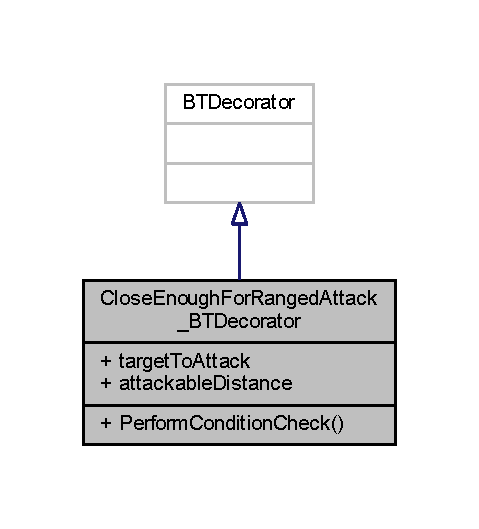
\includegraphics[width=230pt]{class_close_enough_for_ranged_attack___b_t_decorator__inherit__graph}
\end{center}
\end{figure}


Collaboration diagram for Close\+Enough\+For\+Ranged\+Attack\+\_\+\+B\+T\+Decorator\+:
\nopagebreak
\begin{figure}[H]
\begin{center}
\leavevmode
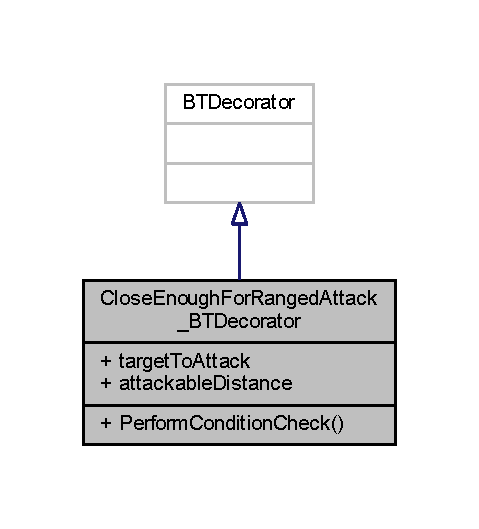
\includegraphics[width=230pt]{class_close_enough_for_ranged_attack___b_t_decorator__coll__graph}
\end{center}
\end{figure}
\subsection*{Public Attributes}
\begin{DoxyCompactItemize}
\item 
Blackboard\+Key\+Selector \hyperlink{class_close_enough_for_ranged_attack___b_t_decorator_a830126ebaba4083a84ea549114ef39d7}{target\+To\+Attack}
\item 
float \hyperlink{class_close_enough_for_ranged_attack___b_t_decorator_a28155d62ff5f45740dad3dfec7254e5e}{attackable\+Distance}
\end{DoxyCompactItemize}


\subsection{Detailed Description}
적 AI 데코레이터 

원거리 공격을 할 수 있는지 판단하기 위해 공격 대상과의 거리를 검사한다. 

\subsection{Member Data Documentation}
\index{Close\+Enough\+For\+Ranged\+Attack\+\_\+\+B\+T\+Decorator@{Close\+Enough\+For\+Ranged\+Attack\+\_\+\+B\+T\+Decorator}!attackable\+Distance@{attackable\+Distance}}
\index{attackable\+Distance@{attackable\+Distance}!Close\+Enough\+For\+Ranged\+Attack\+\_\+\+B\+T\+Decorator@{Close\+Enough\+For\+Ranged\+Attack\+\_\+\+B\+T\+Decorator}}
\subsubsection[{\texorpdfstring{attackable\+Distance}{attackableDistance}}]{\setlength{\rightskip}{0pt plus 5cm}float Close\+Enough\+For\+Ranged\+Attack\+\_\+\+B\+T\+Decorator\+::attackable\+Distance}\hypertarget{class_close_enough_for_ranged_attack___b_t_decorator_a28155d62ff5f45740dad3dfec7254e5e}{}\label{class_close_enough_for_ranged_attack___b_t_decorator_a28155d62ff5f45740dad3dfec7254e5e}
\index{Close\+Enough\+For\+Ranged\+Attack\+\_\+\+B\+T\+Decorator@{Close\+Enough\+For\+Ranged\+Attack\+\_\+\+B\+T\+Decorator}!target\+To\+Attack@{target\+To\+Attack}}
\index{target\+To\+Attack@{target\+To\+Attack}!Close\+Enough\+For\+Ranged\+Attack\+\_\+\+B\+T\+Decorator@{Close\+Enough\+For\+Ranged\+Attack\+\_\+\+B\+T\+Decorator}}
\subsubsection[{\texorpdfstring{target\+To\+Attack}{targetToAttack}}]{\setlength{\rightskip}{0pt plus 5cm}Blackboard\+Key\+Selector Close\+Enough\+For\+Ranged\+Attack\+\_\+\+B\+T\+Decorator\+::target\+To\+Attack}\hypertarget{class_close_enough_for_ranged_attack___b_t_decorator_a830126ebaba4083a84ea549114ef39d7}{}\label{class_close_enough_for_ranged_attack___b_t_decorator_a830126ebaba4083a84ea549114ef39d7}

\hypertarget{class_dec___player_check}{}\section{Dec\+\_\+\+Player\+Check Class Reference}
\label{class_dec___player_check}\index{Dec\+\_\+\+Player\+Check@{Dec\+\_\+\+Player\+Check}}


팀원 AI 데코레이터  




{\ttfamily \#include $<$Dec\+\_\+\+Player\+Check.\+h$>$}



Inheritance diagram for Dec\+\_\+\+Player\+Check\+:\nopagebreak
\begin{figure}[H]
\begin{center}
\leavevmode
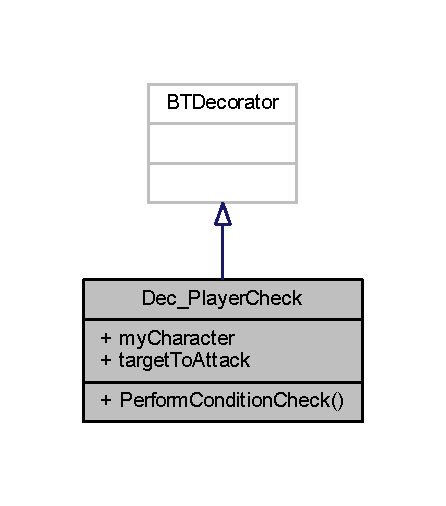
\includegraphics[width=214pt]{class_dec___player_check__inherit__graph}
\end{center}
\end{figure}


Collaboration diagram for Dec\+\_\+\+Player\+Check\+:\nopagebreak
\begin{figure}[H]
\begin{center}
\leavevmode
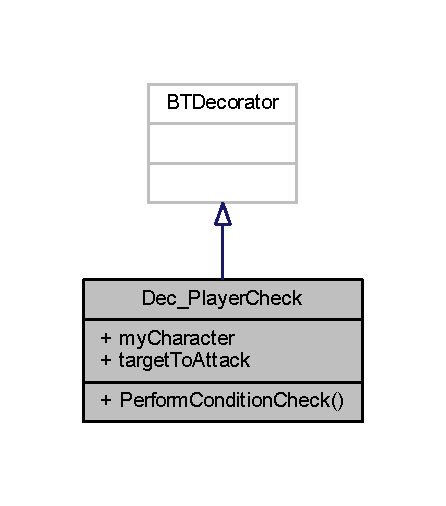
\includegraphics[width=214pt]{class_dec___player_check__coll__graph}
\end{center}
\end{figure}
\subsection*{Public Member Functions}
\begin{DoxyCompactItemize}
\item 
Boolean \hyperlink{class_dec___player_check_a85ba59a2199c42630eb9da3fe398b877}{Perform\+Condition\+Check} (Actor Owner\+Actor)
\begin{DoxyCompactList}\small\item\em 데코레이터 조건 검사 함수 \end{DoxyCompactList}\end{DoxyCompactItemize}
\subsection*{Public Attributes}
\begin{DoxyCompactItemize}
\item 
Blackboard\+Key\+Selector \hyperlink{class_dec___player_check_a3251552a2d0c5c80aa8dea038622f0cb}{my\+Character}
\item 
Blackboard\+Key\+Selector \hyperlink{class_dec___player_check_ad28098e77833bb97a082bb3c7e79c5f4}{target\+To\+Attack}
\end{DoxyCompactItemize}


\subsection{Detailed Description}
팀원 AI 데코레이터 

my\+Character의 값에 따라 플레이어가 A\+I근처에 있는지 확인한다. 

\subsection{Member Function Documentation}
\index{Dec\+\_\+\+Player\+Check@{Dec\+\_\+\+Player\+Check}!Perform\+Condition\+Check@{Perform\+Condition\+Check}}
\index{Perform\+Condition\+Check@{Perform\+Condition\+Check}!Dec\+\_\+\+Player\+Check@{Dec\+\_\+\+Player\+Check}}
\subsubsection[{\texorpdfstring{Perform\+Condition\+Check(\+Actor Owner\+Actor)}{PerformConditionCheck(Actor OwnerActor)}}]{\setlength{\rightskip}{0pt plus 5cm}Boolean Dec\+\_\+\+Player\+Check\+::\+Perform\+Condition\+Check (
\begin{DoxyParamCaption}
\item[{Actor}]{Owner\+Actor}
\end{DoxyParamCaption}
)}\hypertarget{class_dec___player_check_a85ba59a2199c42630eb9da3fe398b877}{}\label{class_dec___player_check_a85ba59a2199c42630eb9da3fe398b877}


데코레이터 조건 검사 함수 

my\+Character변수가 true면 있다고 인식하고 False면 없다고 인식함. 
\begin{DoxyParams}{Parameters}
{\em Owner\+Actor} & AI 컨트롤러. \\
\hline
\end{DoxyParams}


Here is the caller graph for this function\+:
\nopagebreak
\begin{figure}[H]
\begin{center}
\leavevmode
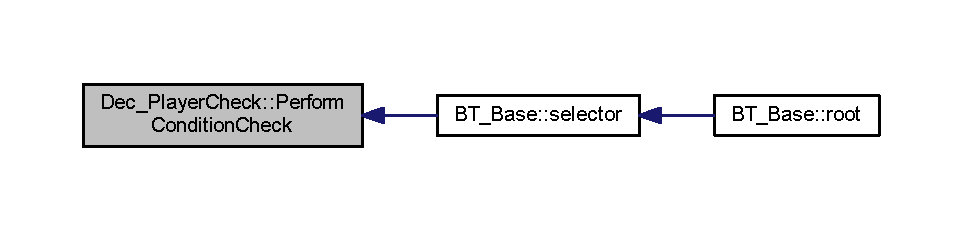
\includegraphics[width=350pt]{class_dec___player_check_a85ba59a2199c42630eb9da3fe398b877_icgraph}
\end{center}
\end{figure}




\subsection{Member Data Documentation}
\index{Dec\+\_\+\+Player\+Check@{Dec\+\_\+\+Player\+Check}!my\+Character@{my\+Character}}
\index{my\+Character@{my\+Character}!Dec\+\_\+\+Player\+Check@{Dec\+\_\+\+Player\+Check}}
\subsubsection[{\texorpdfstring{my\+Character}{myCharacter}}]{\setlength{\rightskip}{0pt plus 5cm}Blackboard\+Key\+Selector Dec\+\_\+\+Player\+Check\+::my\+Character}\hypertarget{class_dec___player_check_a3251552a2d0c5c80aa8dea038622f0cb}{}\label{class_dec___player_check_a3251552a2d0c5c80aa8dea038622f0cb}
\index{Dec\+\_\+\+Player\+Check@{Dec\+\_\+\+Player\+Check}!target\+To\+Attack@{target\+To\+Attack}}
\index{target\+To\+Attack@{target\+To\+Attack}!Dec\+\_\+\+Player\+Check@{Dec\+\_\+\+Player\+Check}}
\subsubsection[{\texorpdfstring{target\+To\+Attack}{targetToAttack}}]{\setlength{\rightskip}{0pt plus 5cm}Blackboard\+Key\+Selector Dec\+\_\+\+Player\+Check\+::target\+To\+Attack}\hypertarget{class_dec___player_check_ad28098e77833bb97a082bb3c7e79c5f4}{}\label{class_dec___player_check_ad28098e77833bb97a082bb3c7e79c5f4}

\hypertarget{class_dec___rotationinit}{}\section{Dec\+\_\+\+Rotationinit Class Reference}
\label{class_dec___rotationinit}\index{Dec\+\_\+\+Rotationinit@{Dec\+\_\+\+Rotationinit}}


팀원 AI 데코레이터  




{\ttfamily \#include $<$Dec\+\_\+\+Rotationinit.\+h$>$}



Inheritance diagram for Dec\+\_\+\+Rotationinit\+:\nopagebreak
\begin{figure}[H]
\begin{center}
\leavevmode
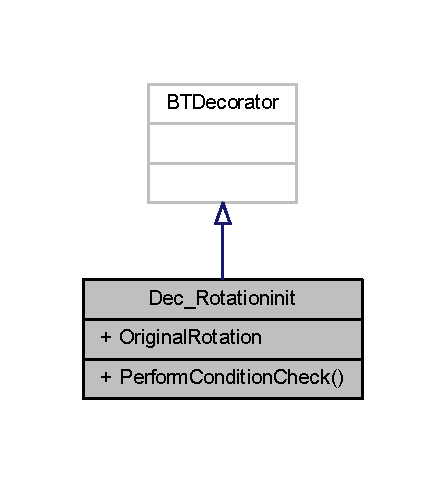
\includegraphics[width=214pt]{class_dec___rotationinit__inherit__graph}
\end{center}
\end{figure}


Collaboration diagram for Dec\+\_\+\+Rotationinit\+:\nopagebreak
\begin{figure}[H]
\begin{center}
\leavevmode
\includegraphics[width=214pt]{class_dec___rotationinit__coll__graph}
\end{center}
\end{figure}
\subsection*{Public Member Functions}
\begin{DoxyCompactItemize}
\item 
Boolean \hyperlink{class_dec___rotationinit_a68df999834394624209d210a21c2d5bd}{Perform\+Condition\+Check} (Actor Owner\+Actor)
\begin{DoxyCompactList}\small\item\em 초기화를 위한 데코레이터 \end{DoxyCompactList}\end{DoxyCompactItemize}
\subsection*{Public Attributes}
\begin{DoxyCompactItemize}
\item 
Blackboard\+Key\+Selector \hyperlink{class_dec___rotationinit_a44b74e55ce2973723fe045806169c6c0}{Original\+Rotation}
\end{DoxyCompactItemize}


\subsection{Detailed Description}
팀원 AI 데코레이터 

A\+I의 초기 Rotation을 초기화를 위한 데코레이터 

\subsection{Member Function Documentation}
\index{Dec\+\_\+\+Rotationinit@{Dec\+\_\+\+Rotationinit}!Perform\+Condition\+Check@{Perform\+Condition\+Check}}
\index{Perform\+Condition\+Check@{Perform\+Condition\+Check}!Dec\+\_\+\+Rotationinit@{Dec\+\_\+\+Rotationinit}}
\subsubsection[{\texorpdfstring{Perform\+Condition\+Check(\+Actor Owner\+Actor)}{PerformConditionCheck(Actor OwnerActor)}}]{\setlength{\rightskip}{0pt plus 5cm}Boolean Dec\+\_\+\+Rotationinit\+::\+Perform\+Condition\+Check (
\begin{DoxyParamCaption}
\item[{Actor}]{Owner\+Actor}
\end{DoxyParamCaption}
)}\hypertarget{class_dec___rotationinit_a68df999834394624209d210a21c2d5bd}{}\label{class_dec___rotationinit_a68df999834394624209d210a21c2d5bd}


초기화를 위한 데코레이터 

단순히 A\+I들의 초기 Rotation을 Set함 
\begin{DoxyParams}{Parameters}
{\em Owner\+Actor} & AI 컨트롤러. \\
\hline
\end{DoxyParams}


Here is the caller graph for this function\+:
\nopagebreak
\begin{figure}[H]
\begin{center}
\leavevmode
\includegraphics[width=350pt]{class_dec___rotationinit_a68df999834394624209d210a21c2d5bd_icgraph}
\end{center}
\end{figure}




\subsection{Member Data Documentation}
\index{Dec\+\_\+\+Rotationinit@{Dec\+\_\+\+Rotationinit}!Original\+Rotation@{Original\+Rotation}}
\index{Original\+Rotation@{Original\+Rotation}!Dec\+\_\+\+Rotationinit@{Dec\+\_\+\+Rotationinit}}
\subsubsection[{\texorpdfstring{Original\+Rotation}{OriginalRotation}}]{\setlength{\rightskip}{0pt plus 5cm}Blackboard\+Key\+Selector Dec\+\_\+\+Rotationinit\+::\+Original\+Rotation}\hypertarget{class_dec___rotationinit_a44b74e55ce2973723fe045806169c6c0}{}\label{class_dec___rotationinit_a44b74e55ce2973723fe045806169c6c0}

\hypertarget{class_enemy___character}{}\section{Enemy\+\_\+\+Character Class Reference}
\label{class_enemy___character}\index{Enemy\+\_\+\+Character@{Enemy\+\_\+\+Character}}


적 기본 클래스.  




{\ttfamily \#include $<$Enemy\+\_\+\+Character.\+h$>$}



Inheritance diagram for Enemy\+\_\+\+Character\+:
\nopagebreak
\begin{figure}[H]
\begin{center}
\leavevmode
\includegraphics[width=350pt]{class_enemy___character__inherit__graph}
\end{center}
\end{figure}


Collaboration diagram for Enemy\+\_\+\+Character\+:
\nopagebreak
\begin{figure}[H]
\begin{center}
\leavevmode
\includegraphics[width=206pt]{class_enemy___character__coll__graph}
\end{center}
\end{figure}
\subsection*{Public Member Functions}
\begin{DoxyCompactItemize}
\item 
Construction \hyperlink{class_enemy___character_a96c9dc103aa4bcb4ee3a5c8d6dfe340b}{Script} ()
\begin{DoxyCompactList}\small\item\em 컨스트럭션 스크립트. \end{DoxyCompactList}\item 
Event\+Graph \hyperlink{class_enemy___character_ae989f213471b46262de4e372ecbe5c63}{Any\+Damage} (float Damage, Object Damage\+Type, Actor Instigated\+By, Actor Damage\+Causer)
\begin{DoxyCompactList}\small\item\em 데미지 처리 이벤트. \end{DoxyCompactList}\item 
void \hyperlink{class_enemy___character_a1a017228dd07231176118c82ea0ae4cf}{on\+Die} ()
\begin{DoxyCompactList}\small\item\em ..... \end{DoxyCompactList}\item 
void \hyperlink{class_enemy___character_abf821a2be938d0686caf45fa6c738af7}{set\+Can\+Attack} (bool \+\_\+can\+\_\+attack)
\begin{DoxyCompactList}\small\item\em ..... \end{DoxyCompactList}\item 
void \hyperlink{class_enemy___character_a74b04f0f28f9122e6474da8ae03abe57}{hit\+Attack} (Hit\+Result \+\_\+hit, Actor \+\_\+other\+\_\+actor)
\begin{DoxyCompactList}\small\item\em ..... \end{DoxyCompactList}\item 
void \hyperlink{class_enemy___character_acafb348c1628d5a141d161c03189b4fe}{on\+Attack} ()
\begin{DoxyCompactList}\small\item\em ..... \end{DoxyCompactList}\item 
void \hyperlink{class_enemy___character_aa4f5af02eb960516ca6134a0e84e958a}{alarm\+Getting\+Attacked} (Actor \+\_\+demage\+Causer)
\begin{DoxyCompactList}\small\item\em ..... \end{DoxyCompactList}\item 
void \hyperlink{class_enemy___character_af291c216d2d7ce2c83e71cb151cf13ee}{receive\+Attack\+Alarm} (Actor \+\_\+demage\+Causer)
\begin{DoxyCompactList}\small\item\em ..... \end{DoxyCompactList}\item 
void \hyperlink{class_enemy___character_a8c8cc52e86cc963f5655b148bd39d27a}{play\+Attack\+Sound} ()
\begin{DoxyCompactList}\small\item\em ..... \end{DoxyCompactList}\item 
void \hyperlink{class_enemy___character_a7e4f2603e52f32f5823ec13e3bfea030}{play\+Die\+Sound} ()
\begin{DoxyCompactList}\small\item\em ..... \end{DoxyCompactList}\item 
void \hyperlink{class_enemy___character_ada6e551c65c0dd91b7e8342036406e7a}{play\+Attack\+Sound2} ()
\begin{DoxyCompactList}\small\item\em ..... \end{DoxyCompactList}\item 
void \hyperlink{class_enemy___character_a0cf94922a5d6b054efaa3a37ec4557e6}{play\+Attack\+Sound3} ()
\begin{DoxyCompactList}\small\item\em ..... \end{DoxyCompactList}\item 
Macros \hyperlink{class_enemy___character_a05b0072de08ac991ff3bc139c4be350f}{is\+Team\+Kill} (bool \+\_\+can\+\_\+teamkill, Actor \+\_\+demage\+\_\+curser)
\begin{DoxyCompactList}\small\item\em ..... \end{DoxyCompactList}\item 
Macros \hyperlink{class_enemy___character_acb2526ab98b23f7928215895caf0532c}{apply\+Demage} (bool \+\_\+demage)
\begin{DoxyCompactList}\small\item\em ..... \end{DoxyCompactList}\end{DoxyCompactItemize}
\subsection*{Public Attributes}
\begin{DoxyCompactItemize}
\item 
float \hyperlink{class_enemy___character_af249f722b34df3e44a6fe14330b99bd4}{hp}
\item 
float \hyperlink{class_enemy___character_aea87cbc161a3dca85393f7da1e4ae923}{D\+E\+M\+A\+GE}
\item 
float \hyperlink{class_enemy___character_a610d52a2f58f031c193b02f36ccaa5e2}{M\+A\+X\+\_\+\+HP}
\item 
bool \hyperlink{class_enemy___character_af40d81990cc8500236418d252857ada0}{can\+\_\+attack}
\end{DoxyCompactItemize}


\subsection{Detailed Description}
적 기본 클래스. 

모든 적들은 해당 클래스를 부모 클래스로 가진다. 

\subsection{Member Function Documentation}
\index{Enemy\+\_\+\+Character@{Enemy\+\_\+\+Character}!alarm\+Getting\+Attacked@{alarm\+Getting\+Attacked}}
\index{alarm\+Getting\+Attacked@{alarm\+Getting\+Attacked}!Enemy\+\_\+\+Character@{Enemy\+\_\+\+Character}}
\subsubsection[{\texorpdfstring{alarm\+Getting\+Attacked(\+Actor \+\_\+demage\+Causer)}{alarmGettingAttacked(Actor _demageCauser)}}]{\setlength{\rightskip}{0pt plus 5cm}void Enemy\+\_\+\+Character\+::alarm\+Getting\+Attacked (
\begin{DoxyParamCaption}
\item[{Actor}]{\+\_\+demage\+Causer}
\end{DoxyParamCaption}
)}\hypertarget{class_enemy___character_aa4f5af02eb960516ca6134a0e84e958a}{}\label{class_enemy___character_aa4f5af02eb960516ca6134a0e84e958a}


..... 

///// 
\begin{DoxyParams}{Parameters}
{\em \+\_\+hit} & //// \\
\hline
{\em \+\_\+other\+\_\+actor} & /// \\
\hline
\end{DoxyParams}


Here is the caller graph for this function\+:\nopagebreak
\begin{figure}[H]
\begin{center}
\leavevmode
\includegraphics[width=350pt]{class_enemy___character_aa4f5af02eb960516ca6134a0e84e958a_icgraph}
\end{center}
\end{figure}


\index{Enemy\+\_\+\+Character@{Enemy\+\_\+\+Character}!Any\+Damage@{Any\+Damage}}
\index{Any\+Damage@{Any\+Damage}!Enemy\+\_\+\+Character@{Enemy\+\_\+\+Character}}
\subsubsection[{\texorpdfstring{Any\+Damage(float Damage, Object Damage\+Type, Actor Instigated\+By, Actor Damage\+Causer)}{AnyDamage(float Damage, Object DamageType, Actor InstigatedBy, Actor DamageCauser)}}]{\setlength{\rightskip}{0pt plus 5cm}Event\+Graph Enemy\+\_\+\+Character\+::\+Any\+Damage (
\begin{DoxyParamCaption}
\item[{float}]{Damage, }
\item[{Object}]{Damage\+Type, }
\item[{Actor}]{Instigated\+By, }
\item[{Actor}]{Damage\+Causer}
\end{DoxyParamCaption}
)}\hypertarget{class_enemy___character_ae989f213471b46262de4e372ecbe5c63}{}\label{class_enemy___character_ae989f213471b46262de4e372ecbe5c63}


데미지 처리 이벤트. 

어떠한 종류의 데미지라도 데미지를 입는다면 들어오는 이벤트다.

팀킬 가능 여부를 체크한 뒤 Demage를 Hp에 적용한다.

데미지 처리 후 죽을 경우 적절한 애니메이션을 실행한다.

주변 동료들에게 공격받은 사실을 알림. 
\begin{DoxyParams}[1]{Parameters}
\textquotesingle{}https\+://docs.\+unrealengine.\+com/latest/\+K\+O\+R/\+Engine/\+Blueprints/\+User\+Guide/\+Events/index.\+html & {\em eventanydamage\textquotesingle{}} & \\
\hline
\end{DoxyParams}


Here is the call graph for this function\+:
\nopagebreak
\begin{figure}[H]
\begin{center}
\leavevmode
\includegraphics[width=350pt]{class_enemy___character_ae989f213471b46262de4e372ecbe5c63_cgraph}
\end{center}
\end{figure}


\index{Enemy\+\_\+\+Character@{Enemy\+\_\+\+Character}!apply\+Demage@{apply\+Demage}}
\index{apply\+Demage@{apply\+Demage}!Enemy\+\_\+\+Character@{Enemy\+\_\+\+Character}}
\subsubsection[{\texorpdfstring{apply\+Demage(bool \+\_\+demage)}{applyDemage(bool _demage)}}]{\setlength{\rightskip}{0pt plus 5cm}Macros Enemy\+\_\+\+Character\+::apply\+Demage (
\begin{DoxyParamCaption}
\item[{bool}]{\+\_\+demage}
\end{DoxyParamCaption}
)}\hypertarget{class_enemy___character_acb2526ab98b23f7928215895caf0532c}{}\label{class_enemy___character_acb2526ab98b23f7928215895caf0532c}


..... 

///// 
\begin{DoxyParams}{Parameters}
{\em \+\_\+hit} & //// \\
\hline
{\em \+\_\+other\+\_\+actor} & /// \\
\hline
\end{DoxyParams}
\index{Enemy\+\_\+\+Character@{Enemy\+\_\+\+Character}!hit\+Attack@{hit\+Attack}}
\index{hit\+Attack@{hit\+Attack}!Enemy\+\_\+\+Character@{Enemy\+\_\+\+Character}}
\subsubsection[{\texorpdfstring{hit\+Attack(\+Hit\+Result \+\_\+hit, Actor \+\_\+other\+\_\+actor)}{hitAttack(HitResult _hit, Actor _other_actor)}}]{\setlength{\rightskip}{0pt plus 5cm}void Enemy\+\_\+\+Character\+::hit\+Attack (
\begin{DoxyParamCaption}
\item[{Hit\+Result}]{\+\_\+hit, }
\item[{Actor}]{\+\_\+other\+\_\+actor}
\end{DoxyParamCaption}
)}\hypertarget{class_enemy___character_a74b04f0f28f9122e6474da8ae03abe57}{}\label{class_enemy___character_a74b04f0f28f9122e6474da8ae03abe57}


..... 

///// 
\begin{DoxyParams}{Parameters}
{\em \+\_\+hit} & //// \\
\hline
{\em \+\_\+other\+\_\+actor} & /// \\
\hline
\end{DoxyParams}
\index{Enemy\+\_\+\+Character@{Enemy\+\_\+\+Character}!is\+Team\+Kill@{is\+Team\+Kill}}
\index{is\+Team\+Kill@{is\+Team\+Kill}!Enemy\+\_\+\+Character@{Enemy\+\_\+\+Character}}
\subsubsection[{\texorpdfstring{is\+Team\+Kill(bool \+\_\+can\+\_\+teamkill, Actor \+\_\+demage\+\_\+curser)}{isTeamKill(bool _can_teamkill, Actor _demage_curser)}}]{\setlength{\rightskip}{0pt plus 5cm}Macros Enemy\+\_\+\+Character\+::is\+Team\+Kill (
\begin{DoxyParamCaption}
\item[{bool}]{\+\_\+can\+\_\+teamkill, }
\item[{Actor}]{\+\_\+demage\+\_\+curser}
\end{DoxyParamCaption}
)}\hypertarget{class_enemy___character_a05b0072de08ac991ff3bc139c4be350f}{}\label{class_enemy___character_a05b0072de08ac991ff3bc139c4be350f}


..... 

///// 
\begin{DoxyParams}{Parameters}
{\em \+\_\+hit} & //// \\
\hline
{\em \+\_\+other\+\_\+actor} & /// \\
\hline
\end{DoxyParams}


Here is the caller graph for this function\+:
\nopagebreak
\begin{figure}[H]
\begin{center}
\leavevmode
\includegraphics[width=350pt]{class_enemy___character_a05b0072de08ac991ff3bc139c4be350f_icgraph}
\end{center}
\end{figure}


\index{Enemy\+\_\+\+Character@{Enemy\+\_\+\+Character}!on\+Attack@{on\+Attack}}
\index{on\+Attack@{on\+Attack}!Enemy\+\_\+\+Character@{Enemy\+\_\+\+Character}}
\subsubsection[{\texorpdfstring{on\+Attack()}{onAttack()}}]{\setlength{\rightskip}{0pt plus 5cm}void Enemy\+\_\+\+Character\+::on\+Attack (
\begin{DoxyParamCaption}
{}
\end{DoxyParamCaption}
)}\hypertarget{class_enemy___character_acafb348c1628d5a141d161c03189b4fe}{}\label{class_enemy___character_acafb348c1628d5a141d161c03189b4fe}


..... 

///// 
\begin{DoxyParams}{Parameters}
{\em \+\_\+hit} & //// \\
\hline
{\em \+\_\+other\+\_\+actor} & /// \\
\hline
\end{DoxyParams}
\index{Enemy\+\_\+\+Character@{Enemy\+\_\+\+Character}!on\+Die@{on\+Die}}
\index{on\+Die@{on\+Die}!Enemy\+\_\+\+Character@{Enemy\+\_\+\+Character}}
\subsubsection[{\texorpdfstring{on\+Die()}{onDie()}}]{\setlength{\rightskip}{0pt plus 5cm}void Enemy\+\_\+\+Character\+::on\+Die (
\begin{DoxyParamCaption}
{}
\end{DoxyParamCaption}
)}\hypertarget{class_enemy___character_a1a017228dd07231176118c82ea0ae4cf}{}\label{class_enemy___character_a1a017228dd07231176118c82ea0ae4cf}


..... 

///// 

Here is the caller graph for this function\+:\nopagebreak
\begin{figure}[H]
\begin{center}
\leavevmode
\includegraphics[width=350pt]{class_enemy___character_a1a017228dd07231176118c82ea0ae4cf_icgraph}
\end{center}
\end{figure}


\index{Enemy\+\_\+\+Character@{Enemy\+\_\+\+Character}!play\+Attack\+Sound@{play\+Attack\+Sound}}
\index{play\+Attack\+Sound@{play\+Attack\+Sound}!Enemy\+\_\+\+Character@{Enemy\+\_\+\+Character}}
\subsubsection[{\texorpdfstring{play\+Attack\+Sound()}{playAttackSound()}}]{\setlength{\rightskip}{0pt plus 5cm}void Enemy\+\_\+\+Character\+::play\+Attack\+Sound (
\begin{DoxyParamCaption}
{}
\end{DoxyParamCaption}
)}\hypertarget{class_enemy___character_a8c8cc52e86cc963f5655b148bd39d27a}{}\label{class_enemy___character_a8c8cc52e86cc963f5655b148bd39d27a}


..... 

///// 
\begin{DoxyParams}{Parameters}
{\em \+\_\+hit} & //// \\
\hline
{\em \+\_\+other\+\_\+actor} & /// \\
\hline
\end{DoxyParams}
\index{Enemy\+\_\+\+Character@{Enemy\+\_\+\+Character}!play\+Attack\+Sound2@{play\+Attack\+Sound2}}
\index{play\+Attack\+Sound2@{play\+Attack\+Sound2}!Enemy\+\_\+\+Character@{Enemy\+\_\+\+Character}}
\subsubsection[{\texorpdfstring{play\+Attack\+Sound2()}{playAttackSound2()}}]{\setlength{\rightskip}{0pt plus 5cm}void Enemy\+\_\+\+Character\+::play\+Attack\+Sound2 (
\begin{DoxyParamCaption}
{}
\end{DoxyParamCaption}
)}\hypertarget{class_enemy___character_ada6e551c65c0dd91b7e8342036406e7a}{}\label{class_enemy___character_ada6e551c65c0dd91b7e8342036406e7a}


..... 

///// 
\begin{DoxyParams}{Parameters}
{\em \+\_\+hit} & //// \\
\hline
{\em \+\_\+other\+\_\+actor} & /// \\
\hline
\end{DoxyParams}
\index{Enemy\+\_\+\+Character@{Enemy\+\_\+\+Character}!play\+Attack\+Sound3@{play\+Attack\+Sound3}}
\index{play\+Attack\+Sound3@{play\+Attack\+Sound3}!Enemy\+\_\+\+Character@{Enemy\+\_\+\+Character}}
\subsubsection[{\texorpdfstring{play\+Attack\+Sound3()}{playAttackSound3()}}]{\setlength{\rightskip}{0pt plus 5cm}void Enemy\+\_\+\+Character\+::play\+Attack\+Sound3 (
\begin{DoxyParamCaption}
{}
\end{DoxyParamCaption}
)}\hypertarget{class_enemy___character_a0cf94922a5d6b054efaa3a37ec4557e6}{}\label{class_enemy___character_a0cf94922a5d6b054efaa3a37ec4557e6}


..... 

///// 
\begin{DoxyParams}{Parameters}
{\em \+\_\+hit} & //// \\
\hline
{\em \+\_\+other\+\_\+actor} & /// \\
\hline
\end{DoxyParams}
\index{Enemy\+\_\+\+Character@{Enemy\+\_\+\+Character}!play\+Die\+Sound@{play\+Die\+Sound}}
\index{play\+Die\+Sound@{play\+Die\+Sound}!Enemy\+\_\+\+Character@{Enemy\+\_\+\+Character}}
\subsubsection[{\texorpdfstring{play\+Die\+Sound()}{playDieSound()}}]{\setlength{\rightskip}{0pt plus 5cm}void Enemy\+\_\+\+Character\+::play\+Die\+Sound (
\begin{DoxyParamCaption}
{}
\end{DoxyParamCaption}
)}\hypertarget{class_enemy___character_a7e4f2603e52f32f5823ec13e3bfea030}{}\label{class_enemy___character_a7e4f2603e52f32f5823ec13e3bfea030}


..... 

///// 
\begin{DoxyParams}{Parameters}
{\em \+\_\+hit} & //// \\
\hline
{\em \+\_\+other\+\_\+actor} & /// \\
\hline
\end{DoxyParams}
\index{Enemy\+\_\+\+Character@{Enemy\+\_\+\+Character}!receive\+Attack\+Alarm@{receive\+Attack\+Alarm}}
\index{receive\+Attack\+Alarm@{receive\+Attack\+Alarm}!Enemy\+\_\+\+Character@{Enemy\+\_\+\+Character}}
\subsubsection[{\texorpdfstring{receive\+Attack\+Alarm(\+Actor \+\_\+demage\+Causer)}{receiveAttackAlarm(Actor _demageCauser)}}]{\setlength{\rightskip}{0pt plus 5cm}void Enemy\+\_\+\+Character\+::receive\+Attack\+Alarm (
\begin{DoxyParamCaption}
\item[{Actor}]{\+\_\+demage\+Causer}
\end{DoxyParamCaption}
)}\hypertarget{class_enemy___character_af291c216d2d7ce2c83e71cb151cf13ee}{}\label{class_enemy___character_af291c216d2d7ce2c83e71cb151cf13ee}


..... 

///// 
\begin{DoxyParams}{Parameters}
{\em \+\_\+hit} & //// \\
\hline
{\em \+\_\+other\+\_\+actor} & /// \\
\hline
\end{DoxyParams}
\index{Enemy\+\_\+\+Character@{Enemy\+\_\+\+Character}!Script@{Script}}
\index{Script@{Script}!Enemy\+\_\+\+Character@{Enemy\+\_\+\+Character}}
\subsubsection[{\texorpdfstring{Script()}{Script()}}]{\setlength{\rightskip}{0pt plus 5cm}Construction Enemy\+\_\+\+Character\+::\+Script (
\begin{DoxyParamCaption}
{}
\end{DoxyParamCaption}
)}\hypertarget{class_enemy___character_a96c9dc103aa4bcb4ee3a5c8d6dfe340b}{}\label{class_enemy___character_a96c9dc103aa4bcb4ee3a5c8d6dfe340b}


컨스트럭션 스크립트. 

HP 초기화

태그(\char`\"{}\+Enemy\char`\"{}) 추가 \index{Enemy\+\_\+\+Character@{Enemy\+\_\+\+Character}!set\+Can\+Attack@{set\+Can\+Attack}}
\index{set\+Can\+Attack@{set\+Can\+Attack}!Enemy\+\_\+\+Character@{Enemy\+\_\+\+Character}}
\subsubsection[{\texorpdfstring{set\+Can\+Attack(bool \+\_\+can\+\_\+attack)}{setCanAttack(bool _can_attack)}}]{\setlength{\rightskip}{0pt plus 5cm}void Enemy\+\_\+\+Character\+::set\+Can\+Attack (
\begin{DoxyParamCaption}
\item[{bool}]{\+\_\+can\+\_\+attack}
\end{DoxyParamCaption}
)}\hypertarget{class_enemy___character_abf821a2be938d0686caf45fa6c738af7}{}\label{class_enemy___character_abf821a2be938d0686caf45fa6c738af7}


..... 

///// 
\begin{DoxyParams}{Parameters}
{\em \+\_\+can\+\_\+attack} & 공격 가능/불가능 상태 세팅. \\
\hline
\end{DoxyParams}


\subsection{Member Data Documentation}
\index{Enemy\+\_\+\+Character@{Enemy\+\_\+\+Character}!can\+\_\+attack@{can\+\_\+attack}}
\index{can\+\_\+attack@{can\+\_\+attack}!Enemy\+\_\+\+Character@{Enemy\+\_\+\+Character}}
\subsubsection[{\texorpdfstring{can\+\_\+attack}{can_attack}}]{\setlength{\rightskip}{0pt plus 5cm}bool Enemy\+\_\+\+Character\+::can\+\_\+attack}\hypertarget{class_enemy___character_af40d81990cc8500236418d252857ada0}{}\label{class_enemy___character_af40d81990cc8500236418d252857ada0}
\index{Enemy\+\_\+\+Character@{Enemy\+\_\+\+Character}!D\+E\+M\+A\+GE@{D\+E\+M\+A\+GE}}
\index{D\+E\+M\+A\+GE@{D\+E\+M\+A\+GE}!Enemy\+\_\+\+Character@{Enemy\+\_\+\+Character}}
\subsubsection[{\texorpdfstring{D\+E\+M\+A\+GE}{DEMAGE}}]{\setlength{\rightskip}{0pt plus 5cm}float Enemy\+\_\+\+Character\+::\+D\+E\+M\+A\+GE}\hypertarget{class_enemy___character_aea87cbc161a3dca85393f7da1e4ae923}{}\label{class_enemy___character_aea87cbc161a3dca85393f7da1e4ae923}
\index{Enemy\+\_\+\+Character@{Enemy\+\_\+\+Character}!hp@{hp}}
\index{hp@{hp}!Enemy\+\_\+\+Character@{Enemy\+\_\+\+Character}}
\subsubsection[{\texorpdfstring{hp}{hp}}]{\setlength{\rightskip}{0pt plus 5cm}float Enemy\+\_\+\+Character\+::hp}\hypertarget{class_enemy___character_af249f722b34df3e44a6fe14330b99bd4}{}\label{class_enemy___character_af249f722b34df3e44a6fe14330b99bd4}
\index{Enemy\+\_\+\+Character@{Enemy\+\_\+\+Character}!M\+A\+X\+\_\+\+HP@{M\+A\+X\+\_\+\+HP}}
\index{M\+A\+X\+\_\+\+HP@{M\+A\+X\+\_\+\+HP}!Enemy\+\_\+\+Character@{Enemy\+\_\+\+Character}}
\subsubsection[{\texorpdfstring{M\+A\+X\+\_\+\+HP}{MAX_HP}}]{\setlength{\rightskip}{0pt plus 5cm}float Enemy\+\_\+\+Character\+::\+M\+A\+X\+\_\+\+HP}\hypertarget{class_enemy___character_a610d52a2f58f031c193b02f36ccaa5e2}{}\label{class_enemy___character_a610d52a2f58f031c193b02f36ccaa5e2}

\hypertarget{class_enemy_a_i_controller___a_i_controller}{}\section{Enemy\+A\+I\+Controller\+\_\+\+A\+I\+Controller Class Reference}
\label{class_enemy_a_i_controller___a_i_controller}\index{Enemy\+A\+I\+Controller\+\_\+\+A\+I\+Controller@{Enemy\+A\+I\+Controller\+\_\+\+A\+I\+Controller}}


적 AI 컨트롤러  




{\ttfamily \#include $<$Enemy\+A\+I\+Controller\+\_\+\+A\+I\+Controller.\+h$>$}



Inheritance diagram for Enemy\+A\+I\+Controller\+\_\+\+A\+I\+Controller\+:
\nopagebreak
\begin{figure}[H]
\begin{center}
\leavevmode
\includegraphics[width=233pt]{class_enemy_a_i_controller___a_i_controller__inherit__graph}
\end{center}
\end{figure}


Collaboration diagram for Enemy\+A\+I\+Controller\+\_\+\+A\+I\+Controller\+:
\nopagebreak
\begin{figure}[H]
\begin{center}
\leavevmode
\includegraphics[width=233pt]{class_enemy_a_i_controller___a_i_controller__coll__graph}
\end{center}
\end{figure}
\subsection*{Public Member Functions}
\begin{DoxyCompactItemize}
\item 
Event\+Graph \hyperlink{class_enemy_a_i_controller___a_i_controller_ae3c3a76e769cd197ed32402d76d7764c}{Begin\+Play} ()
\begin{DoxyCompactList}\small\item\em 게임 시작 이벤트 \end{DoxyCompactList}\end{DoxyCompactItemize}


\subsection{Detailed Description}
적 AI 컨트롤러 

적 AI 캐릭터들을 컨트롤하기 위한 프레임워크 애셋 

\subsection{Member Function Documentation}
\index{Enemy\+A\+I\+Controller\+\_\+\+A\+I\+Controller@{Enemy\+A\+I\+Controller\+\_\+\+A\+I\+Controller}!Begin\+Play@{Begin\+Play}}
\index{Begin\+Play@{Begin\+Play}!Enemy\+A\+I\+Controller\+\_\+\+A\+I\+Controller@{Enemy\+A\+I\+Controller\+\_\+\+A\+I\+Controller}}
\subsubsection[{\texorpdfstring{Begin\+Play()}{BeginPlay()}}]{\setlength{\rightskip}{0pt plus 5cm}Event\+Graph Enemy\+A\+I\+Controller\+\_\+\+A\+I\+Controller\+::\+Begin\+Play (
\begin{DoxyParamCaption}
{}
\end{DoxyParamCaption}
)}\hypertarget{class_enemy_a_i_controller___a_i_controller_ae3c3a76e769cd197ed32402d76d7764c}{}\label{class_enemy_a_i_controller___a_i_controller_ae3c3a76e769cd197ed32402d76d7764c}


게임 시작 이벤트 

적 AI 비헤이비어 트리를 각각의 적 캐릭터들에게 연결시켜준다. 
\hypertarget{class_enemy_attack___b_t_task}{}\section{Enemy\+Attack\+\_\+\+B\+T\+Task Class Reference}
\label{class_enemy_attack___b_t_task}\index{Enemy\+Attack\+\_\+\+B\+T\+Task@{Enemy\+Attack\+\_\+\+B\+T\+Task}}


적 AI 태스크  




{\ttfamily \#include $<$Enemy\+Attack\+\_\+\+B\+T\+Task.\+h$>$}



Inheritance diagram for Enemy\+Attack\+\_\+\+B\+T\+Task\+:\nopagebreak
\begin{figure}[H]
\begin{center}
\leavevmode
\includegraphics[width=194pt]{class_enemy_attack___b_t_task__inherit__graph}
\end{center}
\end{figure}


Collaboration diagram for Enemy\+Attack\+\_\+\+B\+T\+Task\+:\nopagebreak
\begin{figure}[H]
\begin{center}
\leavevmode
\includegraphics[width=194pt]{class_enemy_attack___b_t_task__coll__graph}
\end{center}
\end{figure}
\subsection*{Public Member Functions}
\begin{DoxyCompactItemize}
\item 
Event\+Graph \hyperlink{class_enemy_attack___b_t_task_ace9bb26b7392400fac4a24c736b16116}{Receive\+Tick} ()
\begin{DoxyCompactList}\small\item\em 태스크 틱 이벤트 \end{DoxyCompactList}\item 
Event\+Graph \hyperlink{class_enemy_attack___b_t_task_afbbed53ded3752395a71bf1c86d830d2}{Receive\+Execute} (Actor Owner\+Actor)
\begin{DoxyCompactList}\small\item\em 태스크 실행 이벤트 \end{DoxyCompactList}\end{DoxyCompactItemize}
\subsection*{Public Attributes}
\begin{DoxyCompactItemize}
\item 
Blackboard\+Key\+Selector \hyperlink{class_enemy_attack___b_t_task_a3e66ecf42db2caaa36b45cc0b6116062}{target\+To\+Attack}
\end{DoxyCompactItemize}
\subsection*{Private Attributes}
\begin{DoxyCompactItemize}
\item 
Vector \hyperlink{class_enemy_attack___b_t_task_ab57521e6c6d827822ff6be4f5947e912}{my\+Location}
\item 
Pawn \hyperlink{class_enemy_attack___b_t_task_a547169bbc795a0fc6e6e12601c40cc47}{myself}
\end{DoxyCompactItemize}


\subsection{Detailed Description}
적 AI 태스크 

기본 근접 공격 기능을 한다. 

\subsection{Member Function Documentation}
\index{Enemy\+Attack\+\_\+\+B\+T\+Task@{Enemy\+Attack\+\_\+\+B\+T\+Task}!Receive\+Execute@{Receive\+Execute}}
\index{Receive\+Execute@{Receive\+Execute}!Enemy\+Attack\+\_\+\+B\+T\+Task@{Enemy\+Attack\+\_\+\+B\+T\+Task}}
\subsubsection[{\texorpdfstring{Receive\+Execute(\+Actor Owner\+Actor)}{ReceiveExecute(Actor OwnerActor)}}]{\setlength{\rightskip}{0pt plus 5cm}Event\+Graph Enemy\+Attack\+\_\+\+B\+T\+Task\+::\+Receive\+Execute (
\begin{DoxyParamCaption}
\item[{Actor}]{Owner\+Actor}
\end{DoxyParamCaption}
)}\hypertarget{class_enemy_attack___b_t_task_afbbed53ded3752395a71bf1c86d830d2}{}\label{class_enemy_attack___b_t_task_afbbed53ded3752395a71bf1c86d830d2}


태스크 실행 이벤트 

myself와 my\+Location을 초기화한다. 
\begin{DoxyParams}{Parameters}
{\em Owner\+Actor} & AI 컨트롤러. \\
\hline
\end{DoxyParams}


Here is the caller graph for this function\+:
\nopagebreak
\begin{figure}[H]
\begin{center}
\leavevmode
\includegraphics[width=350pt]{class_enemy_attack___b_t_task_afbbed53ded3752395a71bf1c86d830d2_icgraph}
\end{center}
\end{figure}


\index{Enemy\+Attack\+\_\+\+B\+T\+Task@{Enemy\+Attack\+\_\+\+B\+T\+Task}!Receive\+Tick@{Receive\+Tick}}
\index{Receive\+Tick@{Receive\+Tick}!Enemy\+Attack\+\_\+\+B\+T\+Task@{Enemy\+Attack\+\_\+\+B\+T\+Task}}
\subsubsection[{\texorpdfstring{Receive\+Tick()}{ReceiveTick()}}]{\setlength{\rightskip}{0pt plus 5cm}Event\+Graph Enemy\+Attack\+\_\+\+B\+T\+Task\+::\+Receive\+Tick (
\begin{DoxyParamCaption}
{}
\end{DoxyParamCaption}
)}\hypertarget{class_enemy_attack___b_t_task_ace9bb26b7392400fac4a24c736b16116}{}\label{class_enemy_attack___b_t_task_ace9bb26b7392400fac4a24c736b16116}


태스크 틱 이벤트 

캐릭터가 공격할 대상을 바라보게 하고 on\+Attack을 호출한다. 

Here is the caller graph for this function\+:
\nopagebreak
\begin{figure}[H]
\begin{center}
\leavevmode
\includegraphics[width=350pt]{class_enemy_attack___b_t_task_ace9bb26b7392400fac4a24c736b16116_icgraph}
\end{center}
\end{figure}




\subsection{Member Data Documentation}
\index{Enemy\+Attack\+\_\+\+B\+T\+Task@{Enemy\+Attack\+\_\+\+B\+T\+Task}!my\+Location@{my\+Location}}
\index{my\+Location@{my\+Location}!Enemy\+Attack\+\_\+\+B\+T\+Task@{Enemy\+Attack\+\_\+\+B\+T\+Task}}
\subsubsection[{\texorpdfstring{my\+Location}{myLocation}}]{\setlength{\rightskip}{0pt plus 5cm}Vector Enemy\+Attack\+\_\+\+B\+T\+Task\+::my\+Location\hspace{0.3cm}{\ttfamily [private]}}\hypertarget{class_enemy_attack___b_t_task_ab57521e6c6d827822ff6be4f5947e912}{}\label{class_enemy_attack___b_t_task_ab57521e6c6d827822ff6be4f5947e912}
\index{Enemy\+Attack\+\_\+\+B\+T\+Task@{Enemy\+Attack\+\_\+\+B\+T\+Task}!myself@{myself}}
\index{myself@{myself}!Enemy\+Attack\+\_\+\+B\+T\+Task@{Enemy\+Attack\+\_\+\+B\+T\+Task}}
\subsubsection[{\texorpdfstring{myself}{myself}}]{\setlength{\rightskip}{0pt plus 5cm}Pawn Enemy\+Attack\+\_\+\+B\+T\+Task\+::myself\hspace{0.3cm}{\ttfamily [private]}}\hypertarget{class_enemy_attack___b_t_task_a547169bbc795a0fc6e6e12601c40cc47}{}\label{class_enemy_attack___b_t_task_a547169bbc795a0fc6e6e12601c40cc47}
\index{Enemy\+Attack\+\_\+\+B\+T\+Task@{Enemy\+Attack\+\_\+\+B\+T\+Task}!target\+To\+Attack@{target\+To\+Attack}}
\index{target\+To\+Attack@{target\+To\+Attack}!Enemy\+Attack\+\_\+\+B\+T\+Task@{Enemy\+Attack\+\_\+\+B\+T\+Task}}
\subsubsection[{\texorpdfstring{target\+To\+Attack}{targetToAttack}}]{\setlength{\rightskip}{0pt plus 5cm}Blackboard\+Key\+Selector Enemy\+Attack\+\_\+\+B\+T\+Task\+::target\+To\+Attack}\hypertarget{class_enemy_attack___b_t_task_a3e66ecf42db2caaa36b45cc0b6116062}{}\label{class_enemy_attack___b_t_task_a3e66ecf42db2caaa36b45cc0b6116062}

\hypertarget{class_enemy_blackboard___blackboard}{}\section{Enemy\+Blackboard\+\_\+\+Blackboard Class Reference}
\label{class_enemy_blackboard___blackboard}\index{Enemy\+Blackboard\+\_\+\+Blackboard@{Enemy\+Blackboard\+\_\+\+Blackboard}}


적 AI 블랙보드  




{\ttfamily \#include $<$Enemy\+Blackboard\+\_\+\+Blackboard.\+h$>$}



Inheritance diagram for Enemy\+Blackboard\+\_\+\+Blackboard\+:\nopagebreak
\begin{figure}[H]
\begin{center}
\leavevmode
\includegraphics[width=230pt]{class_enemy_blackboard___blackboard__inherit__graph}
\end{center}
\end{figure}


Collaboration diagram for Enemy\+Blackboard\+\_\+\+Blackboard\+:\nopagebreak
\begin{figure}[H]
\begin{center}
\leavevmode
\includegraphics[width=230pt]{class_enemy_blackboard___blackboard__coll__graph}
\end{center}
\end{figure}
\subsection*{Public Attributes}
\begin{DoxyCompactItemize}
\item 
Object \hyperlink{class_enemy_blackboard___blackboard_a4f1aa5731e916e3a132ab92d54175fb0}{target\+To\+Attack}
\item 
Vector \hyperlink{class_enemy_blackboard___blackboard_a401468bdb3fb40085e8eb2467a33da49}{destination}
\end{DoxyCompactItemize}


\subsection{Detailed Description}
적 AI 블랙보드 

비헤이비어 트리의 흐름을 제어하기 위한 변수들을 모아두는 곳이다. 

\subsection{Member Data Documentation}
\index{Enemy\+Blackboard\+\_\+\+Blackboard@{Enemy\+Blackboard\+\_\+\+Blackboard}!destination@{destination}}
\index{destination@{destination}!Enemy\+Blackboard\+\_\+\+Blackboard@{Enemy\+Blackboard\+\_\+\+Blackboard}}
\subsubsection[{\texorpdfstring{destination}{destination}}]{\setlength{\rightskip}{0pt plus 5cm}Vector Enemy\+Blackboard\+\_\+\+Blackboard\+::destination}\hypertarget{class_enemy_blackboard___blackboard_a401468bdb3fb40085e8eb2467a33da49}{}\label{class_enemy_blackboard___blackboard_a401468bdb3fb40085e8eb2467a33da49}
\index{Enemy\+Blackboard\+\_\+\+Blackboard@{Enemy\+Blackboard\+\_\+\+Blackboard}!target\+To\+Attack@{target\+To\+Attack}}
\index{target\+To\+Attack@{target\+To\+Attack}!Enemy\+Blackboard\+\_\+\+Blackboard@{Enemy\+Blackboard\+\_\+\+Blackboard}}
\subsubsection[{\texorpdfstring{target\+To\+Attack}{targetToAttack}}]{\setlength{\rightskip}{0pt plus 5cm}Object Enemy\+Blackboard\+\_\+\+Blackboard\+::target\+To\+Attack}\hypertarget{class_enemy_blackboard___blackboard_a4f1aa5731e916e3a132ab92d54175fb0}{}\label{class_enemy_blackboard___blackboard_a4f1aa5731e916e3a132ab92d54175fb0}

\hypertarget{class_giant___enemy}{}\section{Giant\+\_\+\+Enemy Class Reference}
\label{class_giant___enemy}\index{Giant\+\_\+\+Enemy@{Giant\+\_\+\+Enemy}}


{\ttfamily \#include $<$Giant\+\_\+\+Enemy.\+h$>$}



Inheritance diagram for Giant\+\_\+\+Enemy\+:\nopagebreak
\begin{figure}[H]
\begin{center}
\leavevmode
\includegraphics[width=196pt]{class_giant___enemy__inherit__graph}
\end{center}
\end{figure}


Collaboration diagram for Giant\+\_\+\+Enemy\+:\nopagebreak
\begin{figure}[H]
\begin{center}
\leavevmode
\includegraphics[width=196pt]{class_giant___enemy__coll__graph}
\end{center}
\end{figure}
\subsection*{Public Member Functions}
\begin{DoxyCompactItemize}
\item 
\hyperlink{class_giant___enemy_a5758c12bf2ab4973307baac4dfc40960}{Giant\+\_\+\+Enemy} ()
\item 
\hyperlink{class_giant___enemy_a199a5437bcee091a90af15d56c5b1bfa}{$\sim$\+Giant\+\_\+\+Enemy} ()
\end{DoxyCompactItemize}


\subsection{Constructor \& Destructor Documentation}
\index{Giant\+\_\+\+Enemy@{Giant\+\_\+\+Enemy}!Giant\+\_\+\+Enemy@{Giant\+\_\+\+Enemy}}
\index{Giant\+\_\+\+Enemy@{Giant\+\_\+\+Enemy}!Giant\+\_\+\+Enemy@{Giant\+\_\+\+Enemy}}
\subsubsection[{\texorpdfstring{Giant\+\_\+\+Enemy()}{Giant_Enemy()}}]{\setlength{\rightskip}{0pt plus 5cm}Giant\+\_\+\+Enemy\+::\+Giant\+\_\+\+Enemy (
\begin{DoxyParamCaption}
{}
\end{DoxyParamCaption}
)}\hypertarget{class_giant___enemy_a5758c12bf2ab4973307baac4dfc40960}{}\label{class_giant___enemy_a5758c12bf2ab4973307baac4dfc40960}
\index{Giant\+\_\+\+Enemy@{Giant\+\_\+\+Enemy}!````~Giant\+\_\+\+Enemy@{$\sim$\+Giant\+\_\+\+Enemy}}
\index{````~Giant\+\_\+\+Enemy@{$\sim$\+Giant\+\_\+\+Enemy}!Giant\+\_\+\+Enemy@{Giant\+\_\+\+Enemy}}
\subsubsection[{\texorpdfstring{$\sim$\+Giant\+\_\+\+Enemy()}{~Giant_Enemy()}}]{\setlength{\rightskip}{0pt plus 5cm}Giant\+\_\+\+Enemy\+::$\sim$\+Giant\+\_\+\+Enemy (
\begin{DoxyParamCaption}
{}
\end{DoxyParamCaption}
)}\hypertarget{class_giant___enemy_a199a5437bcee091a90af15d56c5b1bfa}{}\label{class_giant___enemy_a199a5437bcee091a90af15d56c5b1bfa}

\hypertarget{class_giant_approach___b_t_task}{}\section{Giant\+Approach\+\_\+\+B\+T\+Task Class Reference}
\label{class_giant_approach___b_t_task}\index{Giant\+Approach\+\_\+\+B\+T\+Task@{Giant\+Approach\+\_\+\+B\+T\+Task}}


적 AI 태스크  




{\ttfamily \#include $<$Giant\+Approach\+\_\+\+B\+T\+Task.\+h$>$}



Inheritance diagram for Giant\+Approach\+\_\+\+B\+T\+Task\+:\nopagebreak
\begin{figure}[H]
\begin{center}
\leavevmode
\includegraphics[width=199pt]{class_giant_approach___b_t_task__inherit__graph}
\end{center}
\end{figure}


Collaboration diagram for Giant\+Approach\+\_\+\+B\+T\+Task\+:\nopagebreak
\begin{figure}[H]
\begin{center}
\leavevmode
\includegraphics[width=199pt]{class_giant_approach___b_t_task__coll__graph}
\end{center}
\end{figure}
\subsection*{Public Member Functions}
\begin{DoxyCompactItemize}
\item 
Event\+Graph \hyperlink{class_giant_approach___b_t_task_a5f0940b5b43bd1348e59cb06f0fd7d0e}{Receive\+Execute} (Actor Owner\+Actor)
\begin{DoxyCompactList}\small\item\em 태스크 실행 이벤트 \end{DoxyCompactList}\item 
Event\+Graph \hyperlink{class_giant_approach___b_t_task_adf870b51e3bbfe5895a4265cf1e2cd9c}{Receive\+Abort} ()
\begin{DoxyCompactList}\small\item\em 태스크 중단 이벤트 \end{DoxyCompactList}\end{DoxyCompactItemize}
\subsection*{Public Attributes}
\begin{DoxyCompactItemize}
\item 
Blackboard\+Key\+Selector \hyperlink{class_giant_approach___b_t_task_a6296d9126f5fc2e18266249e91090b18}{target\+To\+Attack}
\end{DoxyCompactItemize}


\subsection{Detailed Description}
적 AI 태스크 

자이언트 전용 대쉬 스킬. 

\subsection{Member Function Documentation}
\index{Giant\+Approach\+\_\+\+B\+T\+Task@{Giant\+Approach\+\_\+\+B\+T\+Task}!Receive\+Abort@{Receive\+Abort}}
\index{Receive\+Abort@{Receive\+Abort}!Giant\+Approach\+\_\+\+B\+T\+Task@{Giant\+Approach\+\_\+\+B\+T\+Task}}
\subsubsection[{\texorpdfstring{Receive\+Abort()}{ReceiveAbort()}}]{\setlength{\rightskip}{0pt plus 5cm}Event\+Graph Giant\+Approach\+\_\+\+B\+T\+Task\+::\+Receive\+Abort (
\begin{DoxyParamCaption}
{}
\end{DoxyParamCaption}
)}\hypertarget{class_giant_approach___b_t_task_adf870b51e3bbfe5895a4265cf1e2cd9c}{}\label{class_giant_approach___b_t_task_adf870b51e3bbfe5895a4265cf1e2cd9c}


태스크 중단 이벤트 

제어 흐름이 끊어지면 대쉬를 끝낸다. 

Here is the caller graph for this function\+:\nopagebreak
\begin{figure}[H]
\begin{center}
\leavevmode
\includegraphics[width=350pt]{class_giant_approach___b_t_task_adf870b51e3bbfe5895a4265cf1e2cd9c_icgraph}
\end{center}
\end{figure}


\index{Giant\+Approach\+\_\+\+B\+T\+Task@{Giant\+Approach\+\_\+\+B\+T\+Task}!Receive\+Execute@{Receive\+Execute}}
\index{Receive\+Execute@{Receive\+Execute}!Giant\+Approach\+\_\+\+B\+T\+Task@{Giant\+Approach\+\_\+\+B\+T\+Task}}
\subsubsection[{\texorpdfstring{Receive\+Execute(\+Actor Owner\+Actor)}{ReceiveExecute(Actor OwnerActor)}}]{\setlength{\rightskip}{0pt plus 5cm}Event\+Graph Giant\+Approach\+\_\+\+B\+T\+Task\+::\+Receive\+Execute (
\begin{DoxyParamCaption}
\item[{Actor}]{Owner\+Actor}
\end{DoxyParamCaption}
)}\hypertarget{class_giant_approach___b_t_task_a5f0940b5b43bd1348e59cb06f0fd7d0e}{}\label{class_giant_approach___b_t_task_a5f0940b5b43bd1348e59cb06f0fd7d0e}


태스크 실행 이벤트 

자이언트가 공격할 대상에게 접근하게 한다.

쿨타임이 아니면 대쉬 스킬을 사용할 수 있다. 
\begin{DoxyParams}{Parameters}
{\em Owner\+Actor} & AI 컨트롤러. \\
\hline
\end{DoxyParams}


Here is the caller graph for this function\+:\nopagebreak
\begin{figure}[H]
\begin{center}
\leavevmode
\includegraphics[width=350pt]{class_giant_approach___b_t_task_a5f0940b5b43bd1348e59cb06f0fd7d0e_icgraph}
\end{center}
\end{figure}




\subsection{Member Data Documentation}
\index{Giant\+Approach\+\_\+\+B\+T\+Task@{Giant\+Approach\+\_\+\+B\+T\+Task}!target\+To\+Attack@{target\+To\+Attack}}
\index{target\+To\+Attack@{target\+To\+Attack}!Giant\+Approach\+\_\+\+B\+T\+Task@{Giant\+Approach\+\_\+\+B\+T\+Task}}
\subsubsection[{\texorpdfstring{target\+To\+Attack}{targetToAttack}}]{\setlength{\rightskip}{0pt plus 5cm}Blackboard\+Key\+Selector Giant\+Approach\+\_\+\+B\+T\+Task\+::target\+To\+Attack}\hypertarget{class_giant_approach___b_t_task_a6296d9126f5fc2e18266249e91090b18}{}\label{class_giant_approach___b_t_task_a6296d9126f5fc2e18266249e91090b18}

\hypertarget{class_giant_behavior_tree___behavior_tree}{}\section{Giant\+Behavior\+Tree\+\_\+\+Behavior\+Tree Class Reference}
\label{class_giant_behavior_tree___behavior_tree}\index{Giant\+Behavior\+Tree\+\_\+\+Behavior\+Tree@{Giant\+Behavior\+Tree\+\_\+\+Behavior\+Tree}}


자이언트의 비헤이비어 트리  




{\ttfamily \#include $<$Giant\+Behavior\+Tree\+\_\+\+Behavior\+Tree.\+h$>$}



Inheritance diagram for Giant\+Behavior\+Tree\+\_\+\+Behavior\+Tree\+:\nopagebreak
\begin{figure}[H]
\begin{center}
\leavevmode
\includegraphics[width=236pt]{class_giant_behavior_tree___behavior_tree__inherit__graph}
\end{center}
\end{figure}


Collaboration diagram for Giant\+Behavior\+Tree\+\_\+\+Behavior\+Tree\+:\nopagebreak
\begin{figure}[H]
\begin{center}
\leavevmode
\includegraphics[width=322pt]{class_giant_behavior_tree___behavior_tree__coll__graph}
\end{center}
\end{figure}
\subsection*{Public Member Functions}
\begin{DoxyCompactItemize}
\item 
void \hyperlink{class_giant_behavior_tree___behavior_tree_a114fdcc0b7b18a7541994c0561d9102d}{root} (\hyperlink{class_enemy_blackboard___blackboard}{Enemy\+Blackboard\+\_\+\+Blackboard} \hyperlink{class_giant_behavior_tree___behavior_tree_a2e26ad9e0c272be24d87a8c1a283895a}{blackboard})
\begin{DoxyCompactList}\small\item\em 루트 노드 \end{DoxyCompactList}\item 
void \hyperlink{class_giant_behavior_tree___behavior_tree_a3eba6d53ad774ed86427759a7437ae2c}{selector} (Object target\+To\+Attack, Vector destination)
\begin{DoxyCompactList}\small\item\em 서비스를 가지는 분기 노드 \end{DoxyCompactList}\item 
void \hyperlink{class_giant_behavior_tree___behavior_tree_ad75d5834908366c41eeb6bab6b409a6b}{idle} (Object target\+To\+Attack)
\begin{DoxyCompactList}\small\item\em 대기 상태 데코레이터 \end{DoxyCompactList}\item 
void \hyperlink{class_giant_behavior_tree___behavior_tree_a07dfd4e1bc0e99b7dabed86be3f19257}{found\+Person} (Object target\+To\+Attack)
\begin{DoxyCompactList}\small\item\em 전투 상태 데코레이터 \end{DoxyCompactList}\item 
void \hyperlink{class_giant_behavior_tree___behavior_tree_ab0fdd6e302f64b84b216cdec31baeb76}{wander} (Vector destination)
\begin{DoxyCompactList}\small\item\em 어슬렁거리기 데코레이터 \end{DoxyCompactList}\item 
void \hyperlink{class_giant_behavior_tree___behavior_tree_af346a6b3b986b6f9092255672e3ce833}{adjacent} (Object target\+To\+Attack)
\begin{DoxyCompactList}\small\item\em 근접 상태 데코레이터 \end{DoxyCompactList}\item 
void \hyperlink{class_giant_behavior_tree___behavior_tree_a3261ee943f9e8045c66bde4489592b42}{near} (Object target\+To\+Attack)
\begin{DoxyCompactList}\small\item\em 가까운 상태 데코레이터 \end{DoxyCompactList}\item 
void \hyperlink{class_giant_behavior_tree___behavior_tree_a6659209498adb2b5f5b9567bd09262f3}{not\+Close} (Object target\+To\+Attack)
\begin{DoxyCompactList}\small\item\em 멀리 떨어진 상태 데코레이터 \end{DoxyCompactList}\item 
void \hyperlink{class_giant_behavior_tree___behavior_tree_a760f8efcdfb234c0063f67b5f785d553}{move\+To} (Vector destination)
\begin{DoxyCompactList}\small\item\em 이동 태스크 \end{DoxyCompactList}\item 
void \hyperlink{class_giant_behavior_tree___behavior_tree_a314e61e0592a048e3158cf8f93cb97c5}{giant\+Melee\+Attack} (Object target\+To\+Attack)
\begin{DoxyCompactList}\small\item\em 근접 공격 태스크 \end{DoxyCompactList}\item 
void \hyperlink{class_giant_behavior_tree___behavior_tree_ac75fb490e2e79c01d24eb4f9a7c6e388}{giant\+Ranged\+Attack} (Object target\+To\+Attack)
\begin{DoxyCompactList}\small\item\em 원거리 공격 태스크 \end{DoxyCompactList}\item 
void \hyperlink{class_giant_behavior_tree___behavior_tree_a0731104134b84cbba860cd168fc3993a}{giant\+Approach} (Object target\+To\+Attack)
\begin{DoxyCompactList}\small\item\em 접근 태스크 \end{DoxyCompactList}\end{DoxyCompactItemize}
\subsection*{Private Attributes}
\begin{DoxyCompactItemize}
\item 
\hyperlink{class_enemy_blackboard___blackboard}{Enemy\+Blackboard\+\_\+\+Blackboard} \hyperlink{class_giant_behavior_tree___behavior_tree_a2e26ad9e0c272be24d87a8c1a283895a}{blackboard}
\end{DoxyCompactItemize}


\subsection{Detailed Description}
자이언트의 비헤이비어 트리 

자이언트의 행동 방식을 컨트롤 한다. 

\subsection{Member Function Documentation}
\index{Giant\+Behavior\+Tree\+\_\+\+Behavior\+Tree@{Giant\+Behavior\+Tree\+\_\+\+Behavior\+Tree}!adjacent@{adjacent}}
\index{adjacent@{adjacent}!Giant\+Behavior\+Tree\+\_\+\+Behavior\+Tree@{Giant\+Behavior\+Tree\+\_\+\+Behavior\+Tree}}
\subsubsection[{\texorpdfstring{adjacent(\+Object target\+To\+Attack)}{adjacent(Object targetToAttack)}}]{\setlength{\rightskip}{0pt plus 5cm}void Giant\+Behavior\+Tree\+\_\+\+Behavior\+Tree\+::adjacent (
\begin{DoxyParamCaption}
\item[{Object}]{target\+To\+Attack}
\end{DoxyParamCaption}
)}\hypertarget{class_giant_behavior_tree___behavior_tree_af346a6b3b986b6f9092255672e3ce833}{}\label{class_giant_behavior_tree___behavior_tree_af346a6b3b986b6f9092255672e3ce833}


근접 상태 데코레이터 

적을 근접 공격할 수 있을 정도로 충분히 가까우면 giant\+Melee\+Attack을 호출한다. 
\begin{DoxyParams}{Parameters}
{\em target\+To\+Attack} & 공격할 대상. \\
\hline
\end{DoxyParams}


Here is the call graph for this function\+:\nopagebreak
\begin{figure}[H]
\begin{center}
\leavevmode
\includegraphics[width=350pt]{class_giant_behavior_tree___behavior_tree_af346a6b3b986b6f9092255672e3ce833_cgraph}
\end{center}
\end{figure}




Here is the caller graph for this function\+:
\nopagebreak
\begin{figure}[H]
\begin{center}
\leavevmode
\includegraphics[width=350pt]{class_giant_behavior_tree___behavior_tree_af346a6b3b986b6f9092255672e3ce833_icgraph}
\end{center}
\end{figure}


\index{Giant\+Behavior\+Tree\+\_\+\+Behavior\+Tree@{Giant\+Behavior\+Tree\+\_\+\+Behavior\+Tree}!found\+Person@{found\+Person}}
\index{found\+Person@{found\+Person}!Giant\+Behavior\+Tree\+\_\+\+Behavior\+Tree@{Giant\+Behavior\+Tree\+\_\+\+Behavior\+Tree}}
\subsubsection[{\texorpdfstring{found\+Person(\+Object target\+To\+Attack)}{foundPerson(Object targetToAttack)}}]{\setlength{\rightskip}{0pt plus 5cm}void Giant\+Behavior\+Tree\+\_\+\+Behavior\+Tree\+::found\+Person (
\begin{DoxyParamCaption}
\item[{Object}]{target\+To\+Attack}
\end{DoxyParamCaption}
)}\hypertarget{class_giant_behavior_tree___behavior_tree_a07dfd4e1bc0e99b7dabed86be3f19257}{}\label{class_giant_behavior_tree___behavior_tree_a07dfd4e1bc0e99b7dabed86be3f19257}


전투 상태 데코레이터 

target\+To\+Attack에 값이 있으면 이쪽으로 분기된다. 
\begin{DoxyParams}{Parameters}
{\em target\+To\+Attack} & 공격할 대상. \\
\hline
\end{DoxyParams}


Here is the call graph for this function\+:
\nopagebreak
\begin{figure}[H]
\begin{center}
\leavevmode
\includegraphics[width=350pt]{class_giant_behavior_tree___behavior_tree_a07dfd4e1bc0e99b7dabed86be3f19257_cgraph}
\end{center}
\end{figure}




Here is the caller graph for this function\+:\nopagebreak
\begin{figure}[H]
\begin{center}
\leavevmode
\includegraphics[width=350pt]{class_giant_behavior_tree___behavior_tree_a07dfd4e1bc0e99b7dabed86be3f19257_icgraph}
\end{center}
\end{figure}


\index{Giant\+Behavior\+Tree\+\_\+\+Behavior\+Tree@{Giant\+Behavior\+Tree\+\_\+\+Behavior\+Tree}!giant\+Approach@{giant\+Approach}}
\index{giant\+Approach@{giant\+Approach}!Giant\+Behavior\+Tree\+\_\+\+Behavior\+Tree@{Giant\+Behavior\+Tree\+\_\+\+Behavior\+Tree}}
\subsubsection[{\texorpdfstring{giant\+Approach(\+Object target\+To\+Attack)}{giantApproach(Object targetToAttack)}}]{\setlength{\rightskip}{0pt plus 5cm}void Giant\+Behavior\+Tree\+\_\+\+Behavior\+Tree\+::giant\+Approach (
\begin{DoxyParamCaption}
\item[{Object}]{target\+To\+Attack}
\end{DoxyParamCaption}
)}\hypertarget{class_giant_behavior_tree___behavior_tree_a0731104134b84cbba860cd168fc3993a}{}\label{class_giant_behavior_tree___behavior_tree_a0731104134b84cbba860cd168fc3993a}


접근 태스크 

공격할 대상에게 접근하는 기능을 수행한다. 
\begin{DoxyParams}{Parameters}
{\em target\+To\+Attack} & 공격할 대상. \\
\hline
\end{DoxyParams}


Here is the call graph for this function\+:\nopagebreak
\begin{figure}[H]
\begin{center}
\leavevmode
\includegraphics[width=350pt]{class_giant_behavior_tree___behavior_tree_a0731104134b84cbba860cd168fc3993a_cgraph}
\end{center}
\end{figure}




Here is the caller graph for this function\+:\nopagebreak
\begin{figure}[H]
\begin{center}
\leavevmode
\includegraphics[width=350pt]{class_giant_behavior_tree___behavior_tree_a0731104134b84cbba860cd168fc3993a_icgraph}
\end{center}
\end{figure}


\index{Giant\+Behavior\+Tree\+\_\+\+Behavior\+Tree@{Giant\+Behavior\+Tree\+\_\+\+Behavior\+Tree}!giant\+Melee\+Attack@{giant\+Melee\+Attack}}
\index{giant\+Melee\+Attack@{giant\+Melee\+Attack}!Giant\+Behavior\+Tree\+\_\+\+Behavior\+Tree@{Giant\+Behavior\+Tree\+\_\+\+Behavior\+Tree}}
\subsubsection[{\texorpdfstring{giant\+Melee\+Attack(\+Object target\+To\+Attack)}{giantMeleeAttack(Object targetToAttack)}}]{\setlength{\rightskip}{0pt plus 5cm}void Giant\+Behavior\+Tree\+\_\+\+Behavior\+Tree\+::giant\+Melee\+Attack (
\begin{DoxyParamCaption}
\item[{Object}]{target\+To\+Attack}
\end{DoxyParamCaption}
)}\hypertarget{class_giant_behavior_tree___behavior_tree_a314e61e0592a048e3158cf8f93cb97c5}{}\label{class_giant_behavior_tree___behavior_tree_a314e61e0592a048e3158cf8f93cb97c5}


근접 공격 태스크 

대상에게 근접 공격 기능을 수행한다. 
\begin{DoxyParams}{Parameters}
{\em target\+To\+Attack} & 공격할 대상. \\
\hline
\end{DoxyParams}


Here is the call graph for this function\+:\nopagebreak
\begin{figure}[H]
\begin{center}
\leavevmode
\includegraphics[width=350pt]{class_giant_behavior_tree___behavior_tree_a314e61e0592a048e3158cf8f93cb97c5_cgraph}
\end{center}
\end{figure}




Here is the caller graph for this function\+:
\nopagebreak
\begin{figure}[H]
\begin{center}
\leavevmode
\includegraphics[width=350pt]{class_giant_behavior_tree___behavior_tree_a314e61e0592a048e3158cf8f93cb97c5_icgraph}
\end{center}
\end{figure}


\index{Giant\+Behavior\+Tree\+\_\+\+Behavior\+Tree@{Giant\+Behavior\+Tree\+\_\+\+Behavior\+Tree}!giant\+Ranged\+Attack@{giant\+Ranged\+Attack}}
\index{giant\+Ranged\+Attack@{giant\+Ranged\+Attack}!Giant\+Behavior\+Tree\+\_\+\+Behavior\+Tree@{Giant\+Behavior\+Tree\+\_\+\+Behavior\+Tree}}
\subsubsection[{\texorpdfstring{giant\+Ranged\+Attack(\+Object target\+To\+Attack)}{giantRangedAttack(Object targetToAttack)}}]{\setlength{\rightskip}{0pt plus 5cm}void Giant\+Behavior\+Tree\+\_\+\+Behavior\+Tree\+::giant\+Ranged\+Attack (
\begin{DoxyParamCaption}
\item[{Object}]{target\+To\+Attack}
\end{DoxyParamCaption}
)}\hypertarget{class_giant_behavior_tree___behavior_tree_ac75fb490e2e79c01d24eb4f9a7c6e388}{}\label{class_giant_behavior_tree___behavior_tree_ac75fb490e2e79c01d24eb4f9a7c6e388}


원거리 공격 태스크 

대상에게 원거리 공격 기능을 수행한다. 
\begin{DoxyParams}{Parameters}
{\em target\+To\+Attack} & 공격할 대상. \\
\hline
\end{DoxyParams}


Here is the call graph for this function\+:\nopagebreak
\begin{figure}[H]
\begin{center}
\leavevmode
\includegraphics[width=350pt]{class_giant_behavior_tree___behavior_tree_ac75fb490e2e79c01d24eb4f9a7c6e388_cgraph}
\end{center}
\end{figure}




Here is the caller graph for this function\+:
\nopagebreak
\begin{figure}[H]
\begin{center}
\leavevmode
\includegraphics[width=350pt]{class_giant_behavior_tree___behavior_tree_ac75fb490e2e79c01d24eb4f9a7c6e388_icgraph}
\end{center}
\end{figure}


\index{Giant\+Behavior\+Tree\+\_\+\+Behavior\+Tree@{Giant\+Behavior\+Tree\+\_\+\+Behavior\+Tree}!idle@{idle}}
\index{idle@{idle}!Giant\+Behavior\+Tree\+\_\+\+Behavior\+Tree@{Giant\+Behavior\+Tree\+\_\+\+Behavior\+Tree}}
\subsubsection[{\texorpdfstring{idle(\+Object target\+To\+Attack)}{idle(Object targetToAttack)}}]{\setlength{\rightskip}{0pt plus 5cm}void Giant\+Behavior\+Tree\+\_\+\+Behavior\+Tree\+::idle (
\begin{DoxyParamCaption}
\item[{Object}]{target\+To\+Attack}
\end{DoxyParamCaption}
)}\hypertarget{class_giant_behavior_tree___behavior_tree_ad75d5834908366c41eeb6bab6b409a6b}{}\label{class_giant_behavior_tree___behavior_tree_ad75d5834908366c41eeb6bab6b409a6b}


대기 상태 데코레이터 

target\+To\+Attack이 비어있을 경우 이쪽으로 분기된다. 
\begin{DoxyParams}{Parameters}
{\em target\+To\+Attack} & 공격할 대상. \\
\hline
\end{DoxyParams}


Here is the call graph for this function\+:\nopagebreak
\begin{figure}[H]
\begin{center}
\leavevmode
\includegraphics[width=350pt]{class_giant_behavior_tree___behavior_tree_ad75d5834908366c41eeb6bab6b409a6b_cgraph}
\end{center}
\end{figure}




Here is the caller graph for this function\+:\nopagebreak
\begin{figure}[H]
\begin{center}
\leavevmode
\includegraphics[width=350pt]{class_giant_behavior_tree___behavior_tree_ad75d5834908366c41eeb6bab6b409a6b_icgraph}
\end{center}
\end{figure}


\index{Giant\+Behavior\+Tree\+\_\+\+Behavior\+Tree@{Giant\+Behavior\+Tree\+\_\+\+Behavior\+Tree}!move\+To@{move\+To}}
\index{move\+To@{move\+To}!Giant\+Behavior\+Tree\+\_\+\+Behavior\+Tree@{Giant\+Behavior\+Tree\+\_\+\+Behavior\+Tree}}
\subsubsection[{\texorpdfstring{move\+To(\+Vector destination)}{moveTo(Vector destination)}}]{\setlength{\rightskip}{0pt plus 5cm}void Giant\+Behavior\+Tree\+\_\+\+Behavior\+Tree\+::move\+To (
\begin{DoxyParamCaption}
\item[{Vector}]{destination}
\end{DoxyParamCaption}
)}\hypertarget{class_giant_behavior_tree___behavior_tree_a760f8efcdfb234c0063f67b5f785d553}{}\label{class_giant_behavior_tree___behavior_tree_a760f8efcdfb234c0063f67b5f785d553}


이동 태스크 

언리얼에서 제공하는 기본 이동 태스크. 
\begin{DoxyParams}{Parameters}
{\em destination} & 이동할 목적지. \\
\hline
\end{DoxyParams}


Here is the call graph for this function\+:\nopagebreak
\begin{figure}[H]
\begin{center}
\leavevmode
\includegraphics[width=350pt]{class_giant_behavior_tree___behavior_tree_a760f8efcdfb234c0063f67b5f785d553_cgraph}
\end{center}
\end{figure}




Here is the caller graph for this function\+:\nopagebreak
\begin{figure}[H]
\begin{center}
\leavevmode
\includegraphics[width=350pt]{class_giant_behavior_tree___behavior_tree_a760f8efcdfb234c0063f67b5f785d553_icgraph}
\end{center}
\end{figure}


\index{Giant\+Behavior\+Tree\+\_\+\+Behavior\+Tree@{Giant\+Behavior\+Tree\+\_\+\+Behavior\+Tree}!near@{near}}
\index{near@{near}!Giant\+Behavior\+Tree\+\_\+\+Behavior\+Tree@{Giant\+Behavior\+Tree\+\_\+\+Behavior\+Tree}}
\subsubsection[{\texorpdfstring{near(\+Object target\+To\+Attack)}{near(Object targetToAttack)}}]{\setlength{\rightskip}{0pt plus 5cm}void Giant\+Behavior\+Tree\+\_\+\+Behavior\+Tree\+::near (
\begin{DoxyParamCaption}
\item[{Object}]{target\+To\+Attack}
\end{DoxyParamCaption}
)}\hypertarget{class_giant_behavior_tree___behavior_tree_a3261ee943f9e8045c66bde4489592b42}{}\label{class_giant_behavior_tree___behavior_tree_a3261ee943f9e8045c66bde4489592b42}


가까운 상태 데코레이터 

적을 원거리 공격할 수 있을 정도로 충분히 가까우면 giant\+Ranged\+Attack을 호출한다. 
\begin{DoxyParams}{Parameters}
{\em target\+To\+Attack} & 공격할 대상. \\
\hline
\end{DoxyParams}


Here is the call graph for this function\+:\nopagebreak
\begin{figure}[H]
\begin{center}
\leavevmode
\includegraphics[width=350pt]{class_giant_behavior_tree___behavior_tree_a3261ee943f9e8045c66bde4489592b42_cgraph}
\end{center}
\end{figure}




Here is the caller graph for this function\+:
\nopagebreak
\begin{figure}[H]
\begin{center}
\leavevmode
\includegraphics[width=350pt]{class_giant_behavior_tree___behavior_tree_a3261ee943f9e8045c66bde4489592b42_icgraph}
\end{center}
\end{figure}


\index{Giant\+Behavior\+Tree\+\_\+\+Behavior\+Tree@{Giant\+Behavior\+Tree\+\_\+\+Behavior\+Tree}!not\+Close@{not\+Close}}
\index{not\+Close@{not\+Close}!Giant\+Behavior\+Tree\+\_\+\+Behavior\+Tree@{Giant\+Behavior\+Tree\+\_\+\+Behavior\+Tree}}
\subsubsection[{\texorpdfstring{not\+Close(\+Object target\+To\+Attack)}{notClose(Object targetToAttack)}}]{\setlength{\rightskip}{0pt plus 5cm}void Giant\+Behavior\+Tree\+\_\+\+Behavior\+Tree\+::not\+Close (
\begin{DoxyParamCaption}
\item[{Object}]{target\+To\+Attack}
\end{DoxyParamCaption}
)}\hypertarget{class_giant_behavior_tree___behavior_tree_a6659209498adb2b5f5b9567bd09262f3}{}\label{class_giant_behavior_tree___behavior_tree_a6659209498adb2b5f5b9567bd09262f3}


멀리 떨어진 상태 데코레이터 

적을 근접 공격할 수 있을 정도로 가깝지 않으면 giant\+Approach를 호출한다. 
\begin{DoxyParams}{Parameters}
{\em target\+To\+Attack} & 공격할 대상. \\
\hline
\end{DoxyParams}


Here is the call graph for this function\+:\nopagebreak
\begin{figure}[H]
\begin{center}
\leavevmode
\includegraphics[width=350pt]{class_giant_behavior_tree___behavior_tree_a6659209498adb2b5f5b9567bd09262f3_cgraph}
\end{center}
\end{figure}




Here is the caller graph for this function\+:\nopagebreak
\begin{figure}[H]
\begin{center}
\leavevmode
\includegraphics[width=350pt]{class_giant_behavior_tree___behavior_tree_a6659209498adb2b5f5b9567bd09262f3_icgraph}
\end{center}
\end{figure}


\index{Giant\+Behavior\+Tree\+\_\+\+Behavior\+Tree@{Giant\+Behavior\+Tree\+\_\+\+Behavior\+Tree}!root@{root}}
\index{root@{root}!Giant\+Behavior\+Tree\+\_\+\+Behavior\+Tree@{Giant\+Behavior\+Tree\+\_\+\+Behavior\+Tree}}
\subsubsection[{\texorpdfstring{root(\+Enemy\+Blackboard\+\_\+\+Blackboard blackboard)}{root(EnemyBlackboard_Blackboard blackboard)}}]{\setlength{\rightskip}{0pt plus 5cm}void Giant\+Behavior\+Tree\+\_\+\+Behavior\+Tree\+::root (
\begin{DoxyParamCaption}
\item[{{\bf Enemy\+Blackboard\+\_\+\+Blackboard}}]{blackboard}
\end{DoxyParamCaption}
)}\hypertarget{class_giant_behavior_tree___behavior_tree_a114fdcc0b7b18a7541994c0561d9102d}{}\label{class_giant_behavior_tree___behavior_tree_a114fdcc0b7b18a7541994c0561d9102d}


루트 노드 

비헤이비어 트리의 루트 노드. 
\begin{DoxyParams}{Parameters}
{\em blackboard} & 비헤이비어 트리에서 사용하는 블랙보드. \\
\hline
\end{DoxyParams}


Here is the call graph for this function\+:
\nopagebreak
\begin{figure}[H]
\begin{center}
\leavevmode
\includegraphics[width=350pt]{class_giant_behavior_tree___behavior_tree_a114fdcc0b7b18a7541994c0561d9102d_cgraph}
\end{center}
\end{figure}


\index{Giant\+Behavior\+Tree\+\_\+\+Behavior\+Tree@{Giant\+Behavior\+Tree\+\_\+\+Behavior\+Tree}!selector@{selector}}
\index{selector@{selector}!Giant\+Behavior\+Tree\+\_\+\+Behavior\+Tree@{Giant\+Behavior\+Tree\+\_\+\+Behavior\+Tree}}
\subsubsection[{\texorpdfstring{selector(\+Object target\+To\+Attack, Vector destination)}{selector(Object targetToAttack, Vector destination)}}]{\setlength{\rightskip}{0pt plus 5cm}void Giant\+Behavior\+Tree\+\_\+\+Behavior\+Tree\+::selector (
\begin{DoxyParamCaption}
\item[{Object}]{target\+To\+Attack, }
\item[{Vector}]{destination}
\end{DoxyParamCaption}
)}\hypertarget{class_giant_behavior_tree___behavior_tree_a3eba6d53ad774ed86427759a7437ae2c}{}\label{class_giant_behavior_tree___behavior_tree_a3eba6d53ad774ed86427759a7437ae2c}


서비스를 가지는 분기 노드 

Scan\+Person\+Character와 Set\+Random\+Destination 서비스를 가지고 있다. 
\begin{DoxyParams}{Parameters}
{\em target\+To\+Attack} & 인간 캐릭터를 발견하면 이 변수에 저장된다. \\
\hline
{\em destination} & 주위 -\/2000 $\sim$ +2000 범위의 랜덤 위치가 저장된다. \\
\hline
\end{DoxyParams}


Here is the call graph for this function\+:
\nopagebreak
\begin{figure}[H]
\begin{center}
\leavevmode
\includegraphics[width=350pt]{class_giant_behavior_tree___behavior_tree_a3eba6d53ad774ed86427759a7437ae2c_cgraph}
\end{center}
\end{figure}




Here is the caller graph for this function\+:\nopagebreak
\begin{figure}[H]
\begin{center}
\leavevmode
\includegraphics[width=350pt]{class_giant_behavior_tree___behavior_tree_a3eba6d53ad774ed86427759a7437ae2c_icgraph}
\end{center}
\end{figure}


\index{Giant\+Behavior\+Tree\+\_\+\+Behavior\+Tree@{Giant\+Behavior\+Tree\+\_\+\+Behavior\+Tree}!wander@{wander}}
\index{wander@{wander}!Giant\+Behavior\+Tree\+\_\+\+Behavior\+Tree@{Giant\+Behavior\+Tree\+\_\+\+Behavior\+Tree}}
\subsubsection[{\texorpdfstring{wander(\+Vector destination)}{wander(Vector destination)}}]{\setlength{\rightskip}{0pt plus 5cm}void Giant\+Behavior\+Tree\+\_\+\+Behavior\+Tree\+::wander (
\begin{DoxyParamCaption}
\item[{Vector}]{destination}
\end{DoxyParamCaption}
)}\hypertarget{class_giant_behavior_tree___behavior_tree_ab0fdd6e302f64b84b216cdec31baeb76}{}\label{class_giant_behavior_tree___behavior_tree_ab0fdd6e302f64b84b216cdec31baeb76}


어슬렁거리기 데코레이터 

공격할 대상이 없고 destination에 값이 있으면 move\+To를 호출한다. 
\begin{DoxyParams}{Parameters}
{\em destination} & 이동할 목적지. \\
\hline
\end{DoxyParams}


Here is the call graph for this function\+:\nopagebreak
\begin{figure}[H]
\begin{center}
\leavevmode
\includegraphics[width=350pt]{class_giant_behavior_tree___behavior_tree_ab0fdd6e302f64b84b216cdec31baeb76_cgraph}
\end{center}
\end{figure}




Here is the caller graph for this function\+:\nopagebreak
\begin{figure}[H]
\begin{center}
\leavevmode
\includegraphics[width=350pt]{class_giant_behavior_tree___behavior_tree_ab0fdd6e302f64b84b216cdec31baeb76_icgraph}
\end{center}
\end{figure}




\subsection{Member Data Documentation}
\index{Giant\+Behavior\+Tree\+\_\+\+Behavior\+Tree@{Giant\+Behavior\+Tree\+\_\+\+Behavior\+Tree}!blackboard@{blackboard}}
\index{blackboard@{blackboard}!Giant\+Behavior\+Tree\+\_\+\+Behavior\+Tree@{Giant\+Behavior\+Tree\+\_\+\+Behavior\+Tree}}
\subsubsection[{\texorpdfstring{blackboard}{blackboard}}]{\setlength{\rightskip}{0pt plus 5cm}{\bf Enemy\+Blackboard\+\_\+\+Blackboard} Giant\+Behavior\+Tree\+\_\+\+Behavior\+Tree\+::blackboard\hspace{0.3cm}{\ttfamily [private]}}\hypertarget{class_giant_behavior_tree___behavior_tree_a2e26ad9e0c272be24d87a8c1a283895a}{}\label{class_giant_behavior_tree___behavior_tree_a2e26ad9e0c272be24d87a8c1a283895a}

\hypertarget{class_giant_close_enough_for_ranged_attack___b_t_decorator}{}\section{Giant\+Close\+Enough\+For\+Ranged\+Attack\+\_\+\+B\+T\+Decorator Class Reference}
\label{class_giant_close_enough_for_ranged_attack___b_t_decorator}\index{Giant\+Close\+Enough\+For\+Ranged\+Attack\+\_\+\+B\+T\+Decorator@{Giant\+Close\+Enough\+For\+Ranged\+Attack\+\_\+\+B\+T\+Decorator}}


적 AI 데코레이터  




{\ttfamily \#include $<$Giant\+Close\+Enough\+For\+Ranged\+Attack\+\_\+\+B\+T\+Decorator.\+h$>$}



Inheritance diagram for Giant\+Close\+Enough\+For\+Ranged\+Attack\+\_\+\+B\+T\+Decorator\+:\nopagebreak
\begin{figure}[H]
\begin{center}
\leavevmode
\includegraphics[width=225pt]{class_giant_close_enough_for_ranged_attack___b_t_decorator__inherit__graph}
\end{center}
\end{figure}


Collaboration diagram for Giant\+Close\+Enough\+For\+Ranged\+Attack\+\_\+\+B\+T\+Decorator\+:\nopagebreak
\begin{figure}[H]
\begin{center}
\leavevmode
\includegraphics[width=225pt]{class_giant_close_enough_for_ranged_attack___b_t_decorator__coll__graph}
\end{center}
\end{figure}
\subsection*{Public Attributes}
\begin{DoxyCompactItemize}
\item 
Blackboard\+Key\+Selector \hyperlink{class_giant_close_enough_for_ranged_attack___b_t_decorator_a1cc248f03397ce0e086ac9b16bd732e1}{target\+To\+Attack}
\item 
float \hyperlink{class_giant_close_enough_for_ranged_attack___b_t_decorator_a994ad90e6d00df363f635eee1fcf2146}{attackable\+Distance}
\end{DoxyCompactItemize}


\subsection{Detailed Description}
적 AI 데코레이터 

자이언트 전용 원거리 공격을 할 수 있는지 판단하기 위해 공격 대상과의 거리를 검사한다. 

\subsection{Member Data Documentation}
\index{Giant\+Close\+Enough\+For\+Ranged\+Attack\+\_\+\+B\+T\+Decorator@{Giant\+Close\+Enough\+For\+Ranged\+Attack\+\_\+\+B\+T\+Decorator}!attackable\+Distance@{attackable\+Distance}}
\index{attackable\+Distance@{attackable\+Distance}!Giant\+Close\+Enough\+For\+Ranged\+Attack\+\_\+\+B\+T\+Decorator@{Giant\+Close\+Enough\+For\+Ranged\+Attack\+\_\+\+B\+T\+Decorator}}
\subsubsection[{\texorpdfstring{attackable\+Distance}{attackableDistance}}]{\setlength{\rightskip}{0pt plus 5cm}float Giant\+Close\+Enough\+For\+Ranged\+Attack\+\_\+\+B\+T\+Decorator\+::attackable\+Distance}\hypertarget{class_giant_close_enough_for_ranged_attack___b_t_decorator_a994ad90e6d00df363f635eee1fcf2146}{}\label{class_giant_close_enough_for_ranged_attack___b_t_decorator_a994ad90e6d00df363f635eee1fcf2146}
\index{Giant\+Close\+Enough\+For\+Ranged\+Attack\+\_\+\+B\+T\+Decorator@{Giant\+Close\+Enough\+For\+Ranged\+Attack\+\_\+\+B\+T\+Decorator}!target\+To\+Attack@{target\+To\+Attack}}
\index{target\+To\+Attack@{target\+To\+Attack}!Giant\+Close\+Enough\+For\+Ranged\+Attack\+\_\+\+B\+T\+Decorator@{Giant\+Close\+Enough\+For\+Ranged\+Attack\+\_\+\+B\+T\+Decorator}}
\subsubsection[{\texorpdfstring{target\+To\+Attack}{targetToAttack}}]{\setlength{\rightskip}{0pt plus 5cm}Blackboard\+Key\+Selector Giant\+Close\+Enough\+For\+Ranged\+Attack\+\_\+\+B\+T\+Decorator\+::target\+To\+Attack}\hypertarget{class_giant_close_enough_for_ranged_attack___b_t_decorator_a1cc248f03397ce0e086ac9b16bd732e1}{}\label{class_giant_close_enough_for_ranged_attack___b_t_decorator_a1cc248f03397ce0e086ac9b16bd732e1}

\hypertarget{class_giant_melee_attack___b_t_task}{}\section{Giant\+Melee\+Attack\+\_\+\+B\+T\+Task Class Reference}
\label{class_giant_melee_attack___b_t_task}\index{Giant\+Melee\+Attack\+\_\+\+B\+T\+Task@{Giant\+Melee\+Attack\+\_\+\+B\+T\+Task}}


적 AI 태스크  




{\ttfamily \#include $<$Giant\+Melee\+Attack\+\_\+\+B\+T\+Task.\+h$>$}



Inheritance diagram for Giant\+Melee\+Attack\+\_\+\+B\+T\+Task\+:\nopagebreak
\begin{figure}[H]
\begin{center}
\leavevmode
\includegraphics[width=213pt]{class_giant_melee_attack___b_t_task__inherit__graph}
\end{center}
\end{figure}


Collaboration diagram for Giant\+Melee\+Attack\+\_\+\+B\+T\+Task\+:\nopagebreak
\begin{figure}[H]
\begin{center}
\leavevmode
\includegraphics[width=213pt]{class_giant_melee_attack___b_t_task__coll__graph}
\end{center}
\end{figure}
\subsection*{Public Attributes}
\begin{DoxyCompactItemize}
\item 
Blackboard\+Key\+Selector \hyperlink{class_giant_melee_attack___b_t_task_ace477d8d2d2c02e1ae5220e36e60b6ac}{target\+To\+Attack}
\end{DoxyCompactItemize}
\subsection*{Private Attributes}
\begin{DoxyCompactItemize}
\item 
Vector \hyperlink{class_giant_melee_attack___b_t_task_a6d7cb8d701fc5a62d10180592a1727bf}{my\+Location}
\item 
Pawn \hyperlink{class_giant_melee_attack___b_t_task_a30dd53d02e844eab55652c2fc628b53c}{myself}
\end{DoxyCompactItemize}


\subsection{Detailed Description}
적 AI 태스크 

자이언트 전용 근접 공격 기능과 범위 공격 스킬. 

\subsection{Member Data Documentation}
\index{Giant\+Melee\+Attack\+\_\+\+B\+T\+Task@{Giant\+Melee\+Attack\+\_\+\+B\+T\+Task}!my\+Location@{my\+Location}}
\index{my\+Location@{my\+Location}!Giant\+Melee\+Attack\+\_\+\+B\+T\+Task@{Giant\+Melee\+Attack\+\_\+\+B\+T\+Task}}
\subsubsection[{\texorpdfstring{my\+Location}{myLocation}}]{\setlength{\rightskip}{0pt plus 5cm}Vector Giant\+Melee\+Attack\+\_\+\+B\+T\+Task\+::my\+Location\hspace{0.3cm}{\ttfamily [private]}}\hypertarget{class_giant_melee_attack___b_t_task_a6d7cb8d701fc5a62d10180592a1727bf}{}\label{class_giant_melee_attack___b_t_task_a6d7cb8d701fc5a62d10180592a1727bf}
\index{Giant\+Melee\+Attack\+\_\+\+B\+T\+Task@{Giant\+Melee\+Attack\+\_\+\+B\+T\+Task}!myself@{myself}}
\index{myself@{myself}!Giant\+Melee\+Attack\+\_\+\+B\+T\+Task@{Giant\+Melee\+Attack\+\_\+\+B\+T\+Task}}
\subsubsection[{\texorpdfstring{myself}{myself}}]{\setlength{\rightskip}{0pt plus 5cm}Pawn Giant\+Melee\+Attack\+\_\+\+B\+T\+Task\+::myself\hspace{0.3cm}{\ttfamily [private]}}\hypertarget{class_giant_melee_attack___b_t_task_a30dd53d02e844eab55652c2fc628b53c}{}\label{class_giant_melee_attack___b_t_task_a30dd53d02e844eab55652c2fc628b53c}
\index{Giant\+Melee\+Attack\+\_\+\+B\+T\+Task@{Giant\+Melee\+Attack\+\_\+\+B\+T\+Task}!target\+To\+Attack@{target\+To\+Attack}}
\index{target\+To\+Attack@{target\+To\+Attack}!Giant\+Melee\+Attack\+\_\+\+B\+T\+Task@{Giant\+Melee\+Attack\+\_\+\+B\+T\+Task}}
\subsubsection[{\texorpdfstring{target\+To\+Attack}{targetToAttack}}]{\setlength{\rightskip}{0pt plus 5cm}Blackboard\+Key\+Selector Giant\+Melee\+Attack\+\_\+\+B\+T\+Task\+::target\+To\+Attack}\hypertarget{class_giant_melee_attack___b_t_task_ace477d8d2d2c02e1ae5220e36e60b6ac}{}\label{class_giant_melee_attack___b_t_task_ace477d8d2d2c02e1ae5220e36e60b6ac}

\hypertarget{class_giant_ranged_attack___b_t_task}{}\section{Giant\+Ranged\+Attack\+\_\+\+B\+T\+Task Class Reference}
\label{class_giant_ranged_attack___b_t_task}\index{Giant\+Ranged\+Attack\+\_\+\+B\+T\+Task@{Giant\+Ranged\+Attack\+\_\+\+B\+T\+Task}}


적 AI 태스크  




{\ttfamily \#include $<$Giant\+Ranged\+Attack\+\_\+\+B\+T\+Task.\+h$>$}



Inheritance diagram for Giant\+Ranged\+Attack\+\_\+\+B\+T\+Task\+:\nopagebreak
\begin{figure}[H]
\begin{center}
\leavevmode
\includegraphics[width=220pt]{class_giant_ranged_attack___b_t_task__inherit__graph}
\end{center}
\end{figure}


Collaboration diagram for Giant\+Ranged\+Attack\+\_\+\+B\+T\+Task\+:\nopagebreak
\begin{figure}[H]
\begin{center}
\leavevmode
\includegraphics[width=220pt]{class_giant_ranged_attack___b_t_task__coll__graph}
\end{center}
\end{figure}
\subsection*{Public Member Functions}
\begin{DoxyCompactItemize}
\item 
Event\+Graph \hyperlink{class_giant_ranged_attack___b_t_task_a08873a799a869f1231ce8d57368ecaad}{Receive\+Tick} ()
\begin{DoxyCompactList}\small\item\em 태스크 틱 이벤트 \end{DoxyCompactList}\item 
Event\+Graph \hyperlink{class_giant_ranged_attack___b_t_task_a88fd0faaab423bc283f4ded45881da6f}{Receive\+Execute} (Actor Owner\+Actor)
\begin{DoxyCompactList}\small\item\em 태스크 실행 이벤트 \end{DoxyCompactList}\end{DoxyCompactItemize}
\subsection*{Public Attributes}
\begin{DoxyCompactItemize}
\item 
Blackboard\+Key\+Selector \hyperlink{class_giant_ranged_attack___b_t_task_ad33350d20d5e08acc84fd65329562c63}{target\+To\+Attack}
\end{DoxyCompactItemize}
\subsection*{Private Attributes}
\begin{DoxyCompactItemize}
\item 
Vector \hyperlink{class_giant_ranged_attack___b_t_task_ad94fd43a278b675d241d6bfbea59efbf}{my\+Location}
\item 
Pawn \hyperlink{class_giant_ranged_attack___b_t_task_a897ee13f9ddeaa6e59a58ac85b7da3db}{myself}
\end{DoxyCompactItemize}


\subsection{Detailed Description}
적 AI 태스크 

자이언트 전용 원거리 공격 스킬. 

\subsection{Member Function Documentation}
\index{Giant\+Ranged\+Attack\+\_\+\+B\+T\+Task@{Giant\+Ranged\+Attack\+\_\+\+B\+T\+Task}!Receive\+Execute@{Receive\+Execute}}
\index{Receive\+Execute@{Receive\+Execute}!Giant\+Ranged\+Attack\+\_\+\+B\+T\+Task@{Giant\+Ranged\+Attack\+\_\+\+B\+T\+Task}}
\subsubsection[{\texorpdfstring{Receive\+Execute(\+Actor Owner\+Actor)}{ReceiveExecute(Actor OwnerActor)}}]{\setlength{\rightskip}{0pt plus 5cm}Event\+Graph Giant\+Ranged\+Attack\+\_\+\+B\+T\+Task\+::\+Receive\+Execute (
\begin{DoxyParamCaption}
\item[{Actor}]{Owner\+Actor}
\end{DoxyParamCaption}
)}\hypertarget{class_giant_ranged_attack___b_t_task_a88fd0faaab423bc283f4ded45881da6f}{}\label{class_giant_ranged_attack___b_t_task_a88fd0faaab423bc283f4ded45881da6f}


태스크 실행 이벤트 

myself와 my\+Location을 초기화한다. 
\begin{DoxyParams}{Parameters}
{\em Owner\+Actor} & AI 컨트롤러. \\
\hline
\end{DoxyParams}


Here is the caller graph for this function\+:
\nopagebreak
\begin{figure}[H]
\begin{center}
\leavevmode
\includegraphics[width=350pt]{class_giant_ranged_attack___b_t_task_a88fd0faaab423bc283f4ded45881da6f_icgraph}
\end{center}
\end{figure}


\index{Giant\+Ranged\+Attack\+\_\+\+B\+T\+Task@{Giant\+Ranged\+Attack\+\_\+\+B\+T\+Task}!Receive\+Tick@{Receive\+Tick}}
\index{Receive\+Tick@{Receive\+Tick}!Giant\+Ranged\+Attack\+\_\+\+B\+T\+Task@{Giant\+Ranged\+Attack\+\_\+\+B\+T\+Task}}
\subsubsection[{\texorpdfstring{Receive\+Tick()}{ReceiveTick()}}]{\setlength{\rightskip}{0pt plus 5cm}Event\+Graph Giant\+Ranged\+Attack\+\_\+\+B\+T\+Task\+::\+Receive\+Tick (
\begin{DoxyParamCaption}
{}
\end{DoxyParamCaption}
)}\hypertarget{class_giant_ranged_attack___b_t_task_a08873a799a869f1231ce8d57368ecaad}{}\label{class_giant_ranged_attack___b_t_task_a08873a799a869f1231ce8d57368ecaad}


태스크 틱 이벤트 

자이언트가 공격할 대상을 바라보게 하고 attack2를 호출한다.

쿨타임이 아니면 범위 공격 스킬을 사용할 수 있다. 

Here is the caller graph for this function\+:
\nopagebreak
\begin{figure}[H]
\begin{center}
\leavevmode
\includegraphics[width=350pt]{class_giant_ranged_attack___b_t_task_a08873a799a869f1231ce8d57368ecaad_icgraph}
\end{center}
\end{figure}




\subsection{Member Data Documentation}
\index{Giant\+Ranged\+Attack\+\_\+\+B\+T\+Task@{Giant\+Ranged\+Attack\+\_\+\+B\+T\+Task}!my\+Location@{my\+Location}}
\index{my\+Location@{my\+Location}!Giant\+Ranged\+Attack\+\_\+\+B\+T\+Task@{Giant\+Ranged\+Attack\+\_\+\+B\+T\+Task}}
\subsubsection[{\texorpdfstring{my\+Location}{myLocation}}]{\setlength{\rightskip}{0pt plus 5cm}Vector Giant\+Ranged\+Attack\+\_\+\+B\+T\+Task\+::my\+Location\hspace{0.3cm}{\ttfamily [private]}}\hypertarget{class_giant_ranged_attack___b_t_task_ad94fd43a278b675d241d6bfbea59efbf}{}\label{class_giant_ranged_attack___b_t_task_ad94fd43a278b675d241d6bfbea59efbf}
\index{Giant\+Ranged\+Attack\+\_\+\+B\+T\+Task@{Giant\+Ranged\+Attack\+\_\+\+B\+T\+Task}!myself@{myself}}
\index{myself@{myself}!Giant\+Ranged\+Attack\+\_\+\+B\+T\+Task@{Giant\+Ranged\+Attack\+\_\+\+B\+T\+Task}}
\subsubsection[{\texorpdfstring{myself}{myself}}]{\setlength{\rightskip}{0pt plus 5cm}Pawn Giant\+Ranged\+Attack\+\_\+\+B\+T\+Task\+::myself\hspace{0.3cm}{\ttfamily [private]}}\hypertarget{class_giant_ranged_attack___b_t_task_a897ee13f9ddeaa6e59a58ac85b7da3db}{}\label{class_giant_ranged_attack___b_t_task_a897ee13f9ddeaa6e59a58ac85b7da3db}
\index{Giant\+Ranged\+Attack\+\_\+\+B\+T\+Task@{Giant\+Ranged\+Attack\+\_\+\+B\+T\+Task}!target\+To\+Attack@{target\+To\+Attack}}
\index{target\+To\+Attack@{target\+To\+Attack}!Giant\+Ranged\+Attack\+\_\+\+B\+T\+Task@{Giant\+Ranged\+Attack\+\_\+\+B\+T\+Task}}
\subsubsection[{\texorpdfstring{target\+To\+Attack}{targetToAttack}}]{\setlength{\rightskip}{0pt plus 5cm}Blackboard\+Key\+Selector Giant\+Ranged\+Attack\+\_\+\+B\+T\+Task\+::target\+To\+Attack}\hypertarget{class_giant_ranged_attack___b_t_task_ad33350d20d5e08acc84fd65329562c63}{}\label{class_giant_ranged_attack___b_t_task_ad33350d20d5e08acc84fd65329562c63}

\hypertarget{class_m4_a1___a_i___person}{}\section{M4\+A1\+\_\+\+A\+I\+\_\+\+Person Class Reference}
\label{class_m4_a1___a_i___person}\index{M4\+A1\+\_\+\+A\+I\+\_\+\+Person@{M4\+A1\+\_\+\+A\+I\+\_\+\+Person}}


{\ttfamily \#include $<$M4\+A1\+\_\+\+A\+I\+\_\+\+Person.\+h$>$}



Inheritance diagram for M4\+A1\+\_\+\+A\+I\+\_\+\+Person\+:\nopagebreak
\begin{figure}[H]
\begin{center}
\leavevmode
\includegraphics[height=550pt]{class_m4_a1___a_i___person__inherit__graph}
\end{center}
\end{figure}


Collaboration diagram for M4\+A1\+\_\+\+A\+I\+\_\+\+Person\+:\nopagebreak
\begin{figure}[H]
\begin{center}
\leavevmode
\includegraphics[height=550pt]{class_m4_a1___a_i___person__coll__graph}
\end{center}
\end{figure}
\subsection*{Public Member Functions}
\begin{DoxyCompactItemize}
\item 
\hyperlink{class_m4_a1___a_i___person_a1a1d34a7ba795d72ec60e73383e566f6}{M4\+A1\+\_\+\+A\+I\+\_\+\+Person} ()
\item 
\hyperlink{class_m4_a1___a_i___person_ab2861a6fd7067eba8bc7656b08987cba}{$\sim$\+M4\+A1\+\_\+\+A\+I\+\_\+\+Person} ()
\end{DoxyCompactItemize}
\subsection*{Additional Inherited Members}


\subsection{Constructor \& Destructor Documentation}
\index{M4\+A1\+\_\+\+A\+I\+\_\+\+Person@{M4\+A1\+\_\+\+A\+I\+\_\+\+Person}!M4\+A1\+\_\+\+A\+I\+\_\+\+Person@{M4\+A1\+\_\+\+A\+I\+\_\+\+Person}}
\index{M4\+A1\+\_\+\+A\+I\+\_\+\+Person@{M4\+A1\+\_\+\+A\+I\+\_\+\+Person}!M4\+A1\+\_\+\+A\+I\+\_\+\+Person@{M4\+A1\+\_\+\+A\+I\+\_\+\+Person}}
\subsubsection[{\texorpdfstring{M4\+A1\+\_\+\+A\+I\+\_\+\+Person()}{M4A1_AI_Person()}}]{\setlength{\rightskip}{0pt plus 5cm}M4\+A1\+\_\+\+A\+I\+\_\+\+Person\+::\+M4\+A1\+\_\+\+A\+I\+\_\+\+Person (
\begin{DoxyParamCaption}
{}
\end{DoxyParamCaption}
)}\hypertarget{class_m4_a1___a_i___person_a1a1d34a7ba795d72ec60e73383e566f6}{}\label{class_m4_a1___a_i___person_a1a1d34a7ba795d72ec60e73383e566f6}
\index{M4\+A1\+\_\+\+A\+I\+\_\+\+Person@{M4\+A1\+\_\+\+A\+I\+\_\+\+Person}!````~M4\+A1\+\_\+\+A\+I\+\_\+\+Person@{$\sim$\+M4\+A1\+\_\+\+A\+I\+\_\+\+Person}}
\index{````~M4\+A1\+\_\+\+A\+I\+\_\+\+Person@{$\sim$\+M4\+A1\+\_\+\+A\+I\+\_\+\+Person}!M4\+A1\+\_\+\+A\+I\+\_\+\+Person@{M4\+A1\+\_\+\+A\+I\+\_\+\+Person}}
\subsubsection[{\texorpdfstring{$\sim$\+M4\+A1\+\_\+\+A\+I\+\_\+\+Person()}{~M4A1_AI_Person()}}]{\setlength{\rightskip}{0pt plus 5cm}M4\+A1\+\_\+\+A\+I\+\_\+\+Person\+::$\sim$\+M4\+A1\+\_\+\+A\+I\+\_\+\+Person (
\begin{DoxyParamCaption}
{}
\end{DoxyParamCaption}
)}\hypertarget{class_m4_a1___a_i___person_ab2861a6fd7067eba8bc7656b08987cba}{}\label{class_m4_a1___a_i___person_ab2861a6fd7067eba8bc7656b08987cba}

\hypertarget{class_m4_a1___weapons}{}\section{M4\+A1\+\_\+\+Weapons Class Reference}
\label{class_m4_a1___weapons}\index{M4\+A1\+\_\+\+Weapons@{M4\+A1\+\_\+\+Weapons}}


{\ttfamily \#include $<$M4\+A1\+\_\+\+Weapons.\+h$>$}



Inheritance diagram for M4\+A1\+\_\+\+Weapons\+:\nopagebreak
\begin{figure}[H]
\begin{center}
\leavevmode
\includegraphics[width=206pt]{class_m4_a1___weapons__inherit__graph}
\end{center}
\end{figure}


Collaboration diagram for M4\+A1\+\_\+\+Weapons\+:\nopagebreak
\begin{figure}[H]
\begin{center}
\leavevmode
\includegraphics[width=206pt]{class_m4_a1___weapons__coll__graph}
\end{center}
\end{figure}
\subsection*{Public Member Functions}
\begin{DoxyCompactItemize}
\item 
\hyperlink{class_m4_a1___weapons_ad2fc508460c93f762d9dfd3ed36e0b1e}{M4\+A1\+\_\+\+Weapons} ()
\item 
\hyperlink{class_m4_a1___weapons_ade0c5fcba12fb2259b5193f972eae0d7}{$\sim$\+M4\+A1\+\_\+\+Weapons} ()
\end{DoxyCompactItemize}
\subsection*{Additional Inherited Members}


\subsection{Constructor \& Destructor Documentation}
\index{M4\+A1\+\_\+\+Weapons@{M4\+A1\+\_\+\+Weapons}!M4\+A1\+\_\+\+Weapons@{M4\+A1\+\_\+\+Weapons}}
\index{M4\+A1\+\_\+\+Weapons@{M4\+A1\+\_\+\+Weapons}!M4\+A1\+\_\+\+Weapons@{M4\+A1\+\_\+\+Weapons}}
\subsubsection[{\texorpdfstring{M4\+A1\+\_\+\+Weapons()}{M4A1_Weapons()}}]{\setlength{\rightskip}{0pt plus 5cm}M4\+A1\+\_\+\+Weapons\+::\+M4\+A1\+\_\+\+Weapons (
\begin{DoxyParamCaption}
{}
\end{DoxyParamCaption}
)}\hypertarget{class_m4_a1___weapons_ad2fc508460c93f762d9dfd3ed36e0b1e}{}\label{class_m4_a1___weapons_ad2fc508460c93f762d9dfd3ed36e0b1e}
\index{M4\+A1\+\_\+\+Weapons@{M4\+A1\+\_\+\+Weapons}!````~M4\+A1\+\_\+\+Weapons@{$\sim$\+M4\+A1\+\_\+\+Weapons}}
\index{````~M4\+A1\+\_\+\+Weapons@{$\sim$\+M4\+A1\+\_\+\+Weapons}!M4\+A1\+\_\+\+Weapons@{M4\+A1\+\_\+\+Weapons}}
\subsubsection[{\texorpdfstring{$\sim$\+M4\+A1\+\_\+\+Weapons()}{~M4A1_Weapons()}}]{\setlength{\rightskip}{0pt plus 5cm}M4\+A1\+\_\+\+Weapons\+::$\sim$\+M4\+A1\+\_\+\+Weapons (
\begin{DoxyParamCaption}
{}
\end{DoxyParamCaption}
)}\hypertarget{class_m4_a1___weapons_ade0c5fcba12fb2259b5193f972eae0d7}{}\label{class_m4_a1___weapons_ade0c5fcba12fb2259b5193f972eae0d7}

\hypertarget{class_person___character}{}\section{Person\+\_\+\+Character Class Reference}
\label{class_person___character}\index{Person\+\_\+\+Character@{Person\+\_\+\+Character}}


아군 캐릭터의 기본형 클래스.  




{\ttfamily \#include $<$Person\+\_\+\+Character.\+h$>$}



Inheritance diagram for Person\+\_\+\+Character\+:\nopagebreak
\begin{figure}[H]
\begin{center}
\leavevmode
\includegraphics[height=550pt]{class_person___character__inherit__graph}
\end{center}
\end{figure}


Collaboration diagram for Person\+\_\+\+Character\+:\nopagebreak
\begin{figure}[H]
\begin{center}
\leavevmode
\includegraphics[height=550pt]{class_person___character__coll__graph}
\end{center}
\end{figure}
\subsection*{Public Member Functions}
\begin{DoxyCompactItemize}
\item 
Construction \hyperlink{class_person___character_adf2ca5624b90380520fc5b3d216f2dc8}{Script} ()
\begin{DoxyCompactList}\small\item\em 컨스트럭션 스크립트. \end{DoxyCompactList}\item 
Event\+Graph \hyperlink{class_person___character_a7e5f3df07b9a156ad0eceb1f6c8e615c}{Any\+Damage} (float Damage, Object Damage\+Type, Actor Instigated\+By, Actor Damage\+Causer)
\begin{DoxyCompactList}\small\item\em 데미지 처리 이벤트. \end{DoxyCompactList}\item 
Event\+Graph \hyperlink{class_person___character_a49833f356173ccfe8857fcbc8e7cf2ad}{Tick} (float Delta\+Seconds)
\begin{DoxyCompactList}\small\item\em Tick 이벤트. \end{DoxyCompactList}\item 
Event\+Graph \hyperlink{class_person___character_a1819d7afedae25bd00de25ee22791bb3}{Begin\+Play} ()
\begin{DoxyCompactList}\small\item\em 시작 이벤트. \end{DoxyCompactList}\item 
Event\+Graph \hyperlink{class_person___character_a72fb7de186f6b9c0091062998673bfe1}{reload\+Dispatcher\+\_\+\+Event} (float \+\_\+delay, int \+\_\+total\+\_\+bullet)
\begin{DoxyCompactList}\small\item\em 재장전을 알리는 이벤트. \end{DoxyCompactList}\item 
Macros \hyperlink{class_person___character_ab255a951f0403e71fac4d2660b692204}{is\+Team\+Kill} (bool \+\_\+can\+\_\+teamkill, Actor \+\_\+demage\+\_\+cursor)
\begin{DoxyCompactList}\small\item\em 팀킬 처리 여부 매크로. \end{DoxyCompactList}\item 
Macros \hyperlink{class_person___character_af2ac7f312634c0f8c2c889cd7dd55c01}{apply\+Demage} (float \+\_\+demage)
\begin{DoxyCompactList}\small\item\em 데미지 처리 매크로. \end{DoxyCompactList}\item 
Macros \hyperlink{class_person___character_a28d17bdc4815d2aa467ddd484a9c273d}{can\+Fire} ()
\begin{DoxyCompactList}\small\item\em 총을 쏠 수 있는 상황인지를 판단. \end{DoxyCompactList}\item 
void \hyperlink{class_person___character_a9207e4718d388fe8af9b5506d1d2e66d}{action\+Jump} (bool \+\_\+on\+\_\+pressed)
\begin{DoxyCompactList}\small\item\em Jump Action 을 처리. \end{DoxyCompactList}\item 
void \hyperlink{class_person___character_a0991452dd5a0ea32b814cb38e1ed7ae7}{action\+Crouch} ()
\begin{DoxyCompactList}\small\item\em 앉는 Action 을 처리. \end{DoxyCompactList}\item 
void \hyperlink{class_person___character_af2570b18cab60a6967ea9572afd34392}{action\+Sprint} (bool \+\_\+on\+\_\+pressed)
\begin{DoxyCompactList}\small\item\em 달리는 Action 을 처리. \end{DoxyCompactList}\item 
void \hyperlink{class_person___character_a5cb52252ac24772509d8277dd45ea16c}{action\+Ironsights} ()
\begin{DoxyCompactList}\small\item\em 정조준 Action 을 처리. \end{DoxyCompactList}\item 
void \hyperlink{class_person___character_aaf8b6f95c71b9a20a78d8e40cc5ebfc1}{get\+Movement\+Values} (bool $\ast$\+\_\+sprint, bool $\ast$\+\_\+crouch, bool $\ast$\+\_\+prone, bool $\ast$\+\_\+jump, bool $\ast$\+\_\+ironsights, Gun\+Type $\ast$\+\_\+gun\+\_\+type)
\begin{DoxyCompactList}\small\item\em 현재 움직임 정보를 한번에 얻을 수 있는 함수. \end{DoxyCompactList}\item 
void \hyperlink{class_person___character_a37cd54aead0c3783a6a0e47382606216}{action\+Fire} (bool \+\_\+on\+\_\+pressed)
\begin{DoxyCompactList}\small\item\em 사격 Action 을 처리. \end{DoxyCompactList}\item 
void \hyperlink{class_person___character_ae24a8beecb67858f956a8d163a4d9333}{ing\+Fire} (float \+\_\+delta\+\_\+seconde)
\begin{DoxyCompactList}\small\item\em 사격중 Aim에 관한 처리를 함. \end{DoxyCompactList}\item 
void \hyperlink{class_person___character_a7d0f5b22056e049f5a46ca0b2abb91ae}{ing\+Fire\+\_\+\+Fire} (Vector \+\_\+start\+\_\+location, Vector \+\_\+end\+\_\+location, float \+\_\+delta\+\_\+seconde)
\begin{DoxyCompactList}\small\item\em 사격중 실제 사격에 관한 처리를 함. \end{DoxyCompactList}\item 
void \hyperlink{class_person___character_a593f0cb97f1f20e42c4ac6642f7dcefe}{action\+Reload} (int \+\_\+total\+\_\+bullet)
\begin{DoxyCompactList}\small\item\em 재장전 Action 을 처리. \end{DoxyCompactList}\item 
void \hyperlink{class_person___character_a5dbcfc49bf5c92294d551a5ead444a80}{end\+Reload\+Anim} ()
\begin{DoxyCompactList}\small\item\em 재장전 애니메이션 완전 종료. \end{DoxyCompactList}\item 
void \hyperlink{class_person___character_adbf33aaddc281c52cc62ab6c59be7b77}{init\+Weapon} ()
\begin{DoxyCompactList}\small\item\em 무기 설정 초기화. \end{DoxyCompactList}\end{DoxyCompactItemize}
\subsection*{Public Attributes}
\begin{DoxyCompactItemize}
\item 
float \hyperlink{class_person___character_ae900d1c986f15b8782b966aadb4f6438}{M\+A\+X\+\_\+\+S\+T\+A\+N\+D\+\_\+\+S\+P\+E\+ED}
\item 
float \hyperlink{class_person___character_a79b89f3df35af4e66e164ab24113602c}{M\+A\+X\+\_\+\+S\+P\+R\+I\+N\+T\+\_\+\+S\+P\+E\+ED}
\item 
float \hyperlink{class_person___character_ac4329d0692d5a4b0909bcf03b71372d8}{M\+A\+X\+\_\+\+C\+R\+O\+U\+C\+H\+\_\+\+S\+P\+E\+ED}
\item 
float \hyperlink{class_person___character_a34724a460f2a77370e18f94745e2ff1f}{M\+A\+X\+\_\+\+S\+T\+A\+N\+D\+\_\+\+I\+R\+O\+N\+S\+I\+G\+H\+T\+S\+\_\+\+S\+P\+E\+ED}
\item 
float \hyperlink{class_person___character_a74127fb1a9316eca1d0c27f41f3ee931}{hp}
\item 
int \hyperlink{class_person___character_a656ddaa791d3bbd4a7e0e8a4acfd01a4}{bullet\+Count}
\item 
bool \hyperlink{class_person___character_afa2a8bdb460adc470c84059b417ee21e}{runing\+\_\+fire}
\item 
\hyperlink{class_weapons___actor}{Weapons\+\_\+\+Actor} \hyperlink{class_person___character_a17d4b4a0e629bbadcaa730305eed57d1}{Gun}
\item 
float \hyperlink{class_person___character_ad1cb8d7e6022b0252d27898b93ff3d87}{M\+A\+X\+\_\+\+HP}
\item 
Hp\+Bar\+Widget \hyperlink{class_person___character_a00bcfae26d753c3c6a539c2c90979a8e}{hp\+\_\+bar}
\item 
bool \hyperlink{class_person___character_a3df071abf16ba980bd55c6d7c8b81fcc}{show\+\_\+hp\+\_\+bar}
\item 
Anim\+Montage \hyperlink{class_person___character_a9e4810e11470421fc099e96537fa1de7}{Anim\+\_\+\+Death}
\item 
Anim\+Montage \hyperlink{class_person___character_a226fe0bb104ba89be5c1eabfa3b7b74a}{Anim\+\_\+\+Fire}
\item 
Anim\+Montage \hyperlink{class_person___character_aab5d72e6f9818ddea6da9517217851d9}{Anim\+\_\+\+Reload}
\item 
Vector2D \hyperlink{class_person___character_adc4d623814ca2a669f2001a9dee85dc2}{screen\+\_\+point}
\end{DoxyCompactItemize}
\subsection*{Private Attributes}
\begin{DoxyCompactItemize}
\item 
bool \hyperlink{class_person___character_ada28cb357a985bcce3ab05cbb107e592}{sprint\+\_\+pressed}
\item 
bool \hyperlink{class_person___character_a06dac4071ddab3cffc34fd3f9f45f82c}{crouch\+\_\+pressed}
\item 
bool \hyperlink{class_person___character_a9abb5b7d14a87eeb58b3860630d61615}{prone\+\_\+pressed}
\item 
bool \hyperlink{class_person___character_ac015d26f3c92ec87951b7a5e6a56a70e}{jump\+\_\+pressed}
\item 
bool \hyperlink{class_person___character_a9a1116d9c0ecc72bb5b8d6b0c4a8d9df}{toggle\+\_\+ironsights}
\item 
bool \hyperlink{class_person___character_a0da4e0f8f35632e924380dc9f129c072}{toggle\+\_\+crouch}
\item 
bool \hyperlink{class_person___character_a2c93570440a103175c39a89de2b29192}{toggle\+Prone}
\item 
bool \hyperlink{class_person___character_a1ed8a1911232a5d7f47773978654d8ea}{disable\+\_\+\+Movement}
\item 
bool \hyperlink{class_person___character_a396ae4ccdc46544ebd28130bec8a46ea}{Ironsights\+\_\+pressed}
\item 
bool \hyperlink{class_person___character_af129a2f5b6da8448d8ee036761b9b737}{is\+\_\+play\+\_\+reload}
\end{DoxyCompactItemize}


\subsection{Detailed Description}
아군 캐릭터의 기본형 클래스. 

사람의 기본적인 움직임을 표현하는 클래스로, player 캐릭터와 AI 캐릭터의 기본적인 움직임을 담당하는 클래스이다. 

\subsection{Member Function Documentation}
\index{Person\+\_\+\+Character@{Person\+\_\+\+Character}!action\+Crouch@{action\+Crouch}}
\index{action\+Crouch@{action\+Crouch}!Person\+\_\+\+Character@{Person\+\_\+\+Character}}
\subsubsection[{\texorpdfstring{action\+Crouch()}{actionCrouch()}}]{\setlength{\rightskip}{0pt plus 5cm}void Person\+\_\+\+Character\+::action\+Crouch (
\begin{DoxyParamCaption}
{}
\end{DoxyParamCaption}
)}\hypertarget{class_person___character_a0991452dd5a0ea32b814cb38e1ed7ae7}{}\label{class_person___character_a0991452dd5a0ea32b814cb38e1ed7ae7}


앉는 Action 을 처리. 

사람의 기본적인 움직임을 표현하는 클래스로, player 캐릭터와 AI 캐릭터의 기본적인 움직임을 담당하는 클래스이다.

토글의 형태로 작동한다. 

Here is the caller graph for this function\+:\nopagebreak
\begin{figure}[H]
\begin{center}
\leavevmode
\includegraphics[width=350pt]{class_person___character_a0991452dd5a0ea32b814cb38e1ed7ae7_icgraph}
\end{center}
\end{figure}


\index{Person\+\_\+\+Character@{Person\+\_\+\+Character}!action\+Fire@{action\+Fire}}
\index{action\+Fire@{action\+Fire}!Person\+\_\+\+Character@{Person\+\_\+\+Character}}
\subsubsection[{\texorpdfstring{action\+Fire(bool \+\_\+on\+\_\+pressed)}{actionFire(bool _on_pressed)}}]{\setlength{\rightskip}{0pt plus 5cm}void Person\+\_\+\+Character\+::action\+Fire (
\begin{DoxyParamCaption}
\item[{bool}]{\+\_\+on\+\_\+pressed}
\end{DoxyParamCaption}
)}\hypertarget{class_person___character_a37cd54aead0c3783a6a0e47382606216}{}\label{class_person___character_a37cd54aead0c3783a6a0e47382606216}


사격 Action 을 처리. 

사람의 기본적인 움직임을 표현하는 클래스로, player 캐릭터와 AI 캐릭터의 기본적인 움직임을 담당하는 클래스이다.

사격 가능 여부를 체크 한 후 사격 함수 호출( ing\+Fire() ). 
\begin{DoxyParams}{Parameters}
{\em \+\_\+on\+\_\+pressed} & 사격키를 눌렀는가에 대한 bool 값. \\
\hline
\end{DoxyParams}


Here is the call graph for this function\+:\nopagebreak
\begin{figure}[H]
\begin{center}
\leavevmode
\includegraphics[width=350pt]{class_person___character_a37cd54aead0c3783a6a0e47382606216_cgraph}
\end{center}
\end{figure}




Here is the caller graph for this function\+:\nopagebreak
\begin{figure}[H]
\begin{center}
\leavevmode
\includegraphics[width=350pt]{class_person___character_a37cd54aead0c3783a6a0e47382606216_icgraph}
\end{center}
\end{figure}


\index{Person\+\_\+\+Character@{Person\+\_\+\+Character}!action\+Ironsights@{action\+Ironsights}}
\index{action\+Ironsights@{action\+Ironsights}!Person\+\_\+\+Character@{Person\+\_\+\+Character}}
\subsubsection[{\texorpdfstring{action\+Ironsights()}{actionIronsights()}}]{\setlength{\rightskip}{0pt plus 5cm}void Person\+\_\+\+Character\+::action\+Ironsights (
\begin{DoxyParamCaption}
{}
\end{DoxyParamCaption}
)}\hypertarget{class_person___character_a5cb52252ac24772509d8277dd45ea16c}{}\label{class_person___character_a5cb52252ac24772509d8277dd45ea16c}


정조준 Action 을 처리. 

사람의 기본적인 움직임을 표현하는 클래스로, player 캐릭터와 AI 캐릭터의 기본적인 움직임을 담당하는 클래스이다.

토글의 형태로 작동한다. 

Here is the call graph for this function\+:\nopagebreak
\begin{figure}[H]
\begin{center}
\leavevmode
\includegraphics[width=350pt]{class_person___character_a5cb52252ac24772509d8277dd45ea16c_cgraph}
\end{center}
\end{figure}




Here is the caller graph for this function\+:\nopagebreak
\begin{figure}[H]
\begin{center}
\leavevmode
\includegraphics[width=350pt]{class_person___character_a5cb52252ac24772509d8277dd45ea16c_icgraph}
\end{center}
\end{figure}


\index{Person\+\_\+\+Character@{Person\+\_\+\+Character}!action\+Jump@{action\+Jump}}
\index{action\+Jump@{action\+Jump}!Person\+\_\+\+Character@{Person\+\_\+\+Character}}
\subsubsection[{\texorpdfstring{action\+Jump(bool \+\_\+on\+\_\+pressed)}{actionJump(bool _on_pressed)}}]{\setlength{\rightskip}{0pt plus 5cm}void Person\+\_\+\+Character\+::action\+Jump (
\begin{DoxyParamCaption}
\item[{bool}]{\+\_\+on\+\_\+pressed}
\end{DoxyParamCaption}
)}\hypertarget{class_person___character_a9207e4718d388fe8af9b5506d1d2e66d}{}\label{class_person___character_a9207e4718d388fe8af9b5506d1d2e66d}


Jump Action 을 처리. 

사람의 기본적인 움직임을 표현하는 클래스로, player 캐릭터와 AI 캐릭터의 기본적인 움직임을 담당하는 클래스이다. 
\begin{DoxyParams}{Parameters}
{\em \+\_\+on\+\_\+pressed} & 점프키를 눌렀는가에 대한 bool 값. \\
\hline
\end{DoxyParams}


Here is the caller graph for this function\+:\nopagebreak
\begin{figure}[H]
\begin{center}
\leavevmode
\includegraphics[width=350pt]{class_person___character_a9207e4718d388fe8af9b5506d1d2e66d_icgraph}
\end{center}
\end{figure}


\index{Person\+\_\+\+Character@{Person\+\_\+\+Character}!action\+Reload@{action\+Reload}}
\index{action\+Reload@{action\+Reload}!Person\+\_\+\+Character@{Person\+\_\+\+Character}}
\subsubsection[{\texorpdfstring{action\+Reload(int \+\_\+total\+\_\+bullet)}{actionReload(int _total_bullet)}}]{\setlength{\rightskip}{0pt plus 5cm}void Person\+\_\+\+Character\+::action\+Reload (
\begin{DoxyParamCaption}
\item[{int}]{\+\_\+total\+\_\+bullet}
\end{DoxyParamCaption}
)}\hypertarget{class_person___character_a593f0cb97f1f20e42c4ac6642f7dcefe}{}\label{class_person___character_a593f0cb97f1f20e42c4ac6642f7dcefe}


재장전 Action 을 처리. 

사람의 기본적인 움직임을 표현하는 클래스로, player 캐릭터와 AI 캐릭터의 기본적인 움직임을 담당하는 클래스이다.

재장전 애니메이션을 재생 후 reload\+Dispatcher\+\_\+\+Event 를 실행한다. 
\begin{DoxyParams}{Parameters}
{\em \+\_\+total\+\_\+bullet} & 소유하고 있는 전체 총알의 수. \\
\hline
\end{DoxyParams}


Here is the call graph for this function\+:\nopagebreak
\begin{figure}[H]
\begin{center}
\leavevmode
\includegraphics[width=350pt]{class_person___character_a593f0cb97f1f20e42c4ac6642f7dcefe_cgraph}
\end{center}
\end{figure}




Here is the caller graph for this function\+:\nopagebreak
\begin{figure}[H]
\begin{center}
\leavevmode
\includegraphics[width=350pt]{class_person___character_a593f0cb97f1f20e42c4ac6642f7dcefe_icgraph}
\end{center}
\end{figure}


\index{Person\+\_\+\+Character@{Person\+\_\+\+Character}!action\+Sprint@{action\+Sprint}}
\index{action\+Sprint@{action\+Sprint}!Person\+\_\+\+Character@{Person\+\_\+\+Character}}
\subsubsection[{\texorpdfstring{action\+Sprint(bool \+\_\+on\+\_\+pressed)}{actionSprint(bool _on_pressed)}}]{\setlength{\rightskip}{0pt plus 5cm}void Person\+\_\+\+Character\+::action\+Sprint (
\begin{DoxyParamCaption}
\item[{bool}]{\+\_\+on\+\_\+pressed}
\end{DoxyParamCaption}
)}\hypertarget{class_person___character_af2570b18cab60a6967ea9572afd34392}{}\label{class_person___character_af2570b18cab60a6967ea9572afd34392}


달리는 Action 을 처리. 

사람의 기본적인 움직임을 표현하는 클래스로, player 캐릭터와 AI 캐릭터의 기본적인 움직임을 담당하는 클래스이다. 
\begin{DoxyParams}{Parameters}
{\em \+\_\+on\+\_\+pressed} & 달리기키를 눌렀는가에 대한 bool 값. \\
\hline
\end{DoxyParams}


Here is the caller graph for this function\+:\nopagebreak
\begin{figure}[H]
\begin{center}
\leavevmode
\includegraphics[width=350pt]{class_person___character_af2570b18cab60a6967ea9572afd34392_icgraph}
\end{center}
\end{figure}


\index{Person\+\_\+\+Character@{Person\+\_\+\+Character}!Any\+Damage@{Any\+Damage}}
\index{Any\+Damage@{Any\+Damage}!Person\+\_\+\+Character@{Person\+\_\+\+Character}}
\subsubsection[{\texorpdfstring{Any\+Damage(float Damage, Object Damage\+Type, Actor Instigated\+By, Actor Damage\+Causer)}{AnyDamage(float Damage, Object DamageType, Actor InstigatedBy, Actor DamageCauser)}}]{\setlength{\rightskip}{0pt plus 5cm}Event\+Graph Person\+\_\+\+Character\+::\+Any\+Damage (
\begin{DoxyParamCaption}
\item[{float}]{Damage, }
\item[{Object}]{Damage\+Type, }
\item[{Actor}]{Instigated\+By, }
\item[{Actor}]{Damage\+Causer}
\end{DoxyParamCaption}
)}\hypertarget{class_person___character_a7e5f3df07b9a156ad0eceb1f6c8e615c}{}\label{class_person___character_a7e5f3df07b9a156ad0eceb1f6c8e615c}


데미지 처리 이벤트. 

어떠한 종류의 데미지라도 데미지를 입는다면 들어오는 이벤트다.

팀킬 가능 여부를 체크한 뒤 Demage를 Hp에 적용한다.

데미지 처리 후 죽을 경우 적절한 애니메이션을 실행한다. 
\begin{DoxyParams}[1]{Parameters}
\textquotesingle{}https\+://docs.\+unrealengine.\+com/latest/\+K\+O\+R/\+Engine/\+Blueprints/\+User\+Guide/\+Events/index.\+html & {\em eventanydamage\textquotesingle{}} & \\
\hline
\end{DoxyParams}
\index{Person\+\_\+\+Character@{Person\+\_\+\+Character}!apply\+Demage@{apply\+Demage}}
\index{apply\+Demage@{apply\+Demage}!Person\+\_\+\+Character@{Person\+\_\+\+Character}}
\subsubsection[{\texorpdfstring{apply\+Demage(float \+\_\+demage)}{applyDemage(float _demage)}}]{\setlength{\rightskip}{0pt plus 5cm}Macros Person\+\_\+\+Character\+::apply\+Demage (
\begin{DoxyParamCaption}
\item[{float}]{\+\_\+demage}
\end{DoxyParamCaption}
)}\hypertarget{class_person___character_af2ac7f312634c0f8c2c889cd7dd55c01}{}\label{class_person___character_af2ac7f312634c0f8c2c889cd7dd55c01}


데미지 처리 매크로. 

받은 데미지 만큼 Hp를 소모하고, 죽었는지를 판단한다. 
\begin{DoxyParams}{Parameters}
{\em \+\_\+demage} & 받은 데미지. \\
\hline
\end{DoxyParams}
\index{Person\+\_\+\+Character@{Person\+\_\+\+Character}!Begin\+Play@{Begin\+Play}}
\index{Begin\+Play@{Begin\+Play}!Person\+\_\+\+Character@{Person\+\_\+\+Character}}
\subsubsection[{\texorpdfstring{Begin\+Play()}{BeginPlay()}}]{\setlength{\rightskip}{0pt plus 5cm}Event\+Graph Person\+\_\+\+Character\+::\+Begin\+Play (
\begin{DoxyParamCaption}
{}
\end{DoxyParamCaption}
)}\hypertarget{class_person___character_a1819d7afedae25bd00de25ee22791bb3}{}\label{class_person___character_a1819d7afedae25bd00de25ee22791bb3}


시작 이벤트. 

블루프린트가 시작 될 때 실행되는 이벤트.

무기(총)의 정보를 초기화 한다.

디버깅용 Hp Bar를 표시여부를 설정한다.

reload\+Dispatcher\+\_\+\+Event를 생성한다. 
\begin{DoxyParams}[1]{Parameters}
\textquotesingle{}https\+://docs.\+unrealengine.\+com/latest/\+K\+O\+R/\+Engine/\+Blueprints/\+User\+Guide/\+Events/index.\+html & {\em eventbeginplay\textquotesingle{}} & \\
\hline
\end{DoxyParams}


Here is the call graph for this function\+:\nopagebreak
\begin{figure}[H]
\begin{center}
\leavevmode
\includegraphics[width=350pt]{class_person___character_a1819d7afedae25bd00de25ee22791bb3_cgraph}
\end{center}
\end{figure}


\index{Person\+\_\+\+Character@{Person\+\_\+\+Character}!can\+Fire@{can\+Fire}}
\index{can\+Fire@{can\+Fire}!Person\+\_\+\+Character@{Person\+\_\+\+Character}}
\subsubsection[{\texorpdfstring{can\+Fire()}{canFire()}}]{\setlength{\rightskip}{0pt plus 5cm}Macros Person\+\_\+\+Character\+::can\+Fire (
\begin{DoxyParamCaption}
{}
\end{DoxyParamCaption}
)}\hypertarget{class_person___character_a28d17bdc4815d2aa467ddd484a9c273d}{}\label{class_person___character_a28d17bdc4815d2aa467ddd484a9c273d}


총을 쏠 수 있는 상황인지를 판단. 

재장전 애니메이션을 실행 중 이거나, 달리는 중에는 총을 쏠 수 없다. \begin{DoxyReturn}{Returns}
총을 쏠 수 있으면 \char`\"{}true\char`\"{}를 리턴한다. 
\end{DoxyReturn}


Here is the caller graph for this function\+:\nopagebreak
\begin{figure}[H]
\begin{center}
\leavevmode
\includegraphics[width=350pt]{class_person___character_a28d17bdc4815d2aa467ddd484a9c273d_icgraph}
\end{center}
\end{figure}


\index{Person\+\_\+\+Character@{Person\+\_\+\+Character}!end\+Reload\+Anim@{end\+Reload\+Anim}}
\index{end\+Reload\+Anim@{end\+Reload\+Anim}!Person\+\_\+\+Character@{Person\+\_\+\+Character}}
\subsubsection[{\texorpdfstring{end\+Reload\+Anim()}{endReloadAnim()}}]{\setlength{\rightskip}{0pt plus 5cm}void Person\+\_\+\+Character\+::end\+Reload\+Anim (
\begin{DoxyParamCaption}
{}
\end{DoxyParamCaption}
)}\hypertarget{class_person___character_a5dbcfc49bf5c92294d551a5ead444a80}{}\label{class_person___character_a5dbcfc49bf5c92294d551a5ead444a80}


재장전 애니메이션 완전 종료. 

재장전 애니메이션이 완전히 종료된 상황으로, 현재 클래스(\+Person\+\_\+\+Character)를 상속받은 자식 클래스에서 오버라이드하여 사용한다. 

Here is the caller graph for this function\+:\nopagebreak
\begin{figure}[H]
\begin{center}
\leavevmode
\includegraphics[width=350pt]{class_person___character_a5dbcfc49bf5c92294d551a5ead444a80_icgraph}
\end{center}
\end{figure}


\index{Person\+\_\+\+Character@{Person\+\_\+\+Character}!get\+Movement\+Values@{get\+Movement\+Values}}
\index{get\+Movement\+Values@{get\+Movement\+Values}!Person\+\_\+\+Character@{Person\+\_\+\+Character}}
\subsubsection[{\texorpdfstring{get\+Movement\+Values(bool $\ast$\+\_\+sprint, bool $\ast$\+\_\+crouch, bool $\ast$\+\_\+prone, bool $\ast$\+\_\+jump, bool $\ast$\+\_\+ironsights, Gun\+Type $\ast$\+\_\+gun\+\_\+type)}{getMovementValues(bool *_sprint, bool *_crouch, bool *_prone, bool *_jump, bool *_ironsights, GunType *_gun_type)}}]{\setlength{\rightskip}{0pt plus 5cm}void Person\+\_\+\+Character\+::get\+Movement\+Values (
\begin{DoxyParamCaption}
\item[{bool $\ast$}]{\+\_\+sprint, }
\item[{bool $\ast$}]{\+\_\+crouch, }
\item[{bool $\ast$}]{\+\_\+prone, }
\item[{bool $\ast$}]{\+\_\+jump, }
\item[{bool $\ast$}]{\+\_\+ironsights, }
\item[{Gun\+Type $\ast$}]{\+\_\+gun\+\_\+type}
\end{DoxyParamCaption}
)}\hypertarget{class_person___character_aaf8b6f95c71b9a20a78d8e40cc5ebfc1}{}\label{class_person___character_aaf8b6f95c71b9a20a78d8e40cc5ebfc1}


현재 움직임 정보를 한번에 얻을 수 있는 함수. 

애니메이션 처리를 돕기 위해 현재 움직임에 대한 정보를 한꺼번에 얻을 수 있는 함수이다. \begin{DoxyReturn}{Returns}
\+\_\+sprint, \+\_\+crouch, \+\_\+prone, \+\_\+jump, \+\_\+ironsights 캐릭터의 현재 행동을 알 수 있다. 

\+\_\+gun\+\_\+type 총기 종류 (서브머신건, 샷건, 스나이퍼건) 를 알 수 있다. 
\end{DoxyReturn}
\index{Person\+\_\+\+Character@{Person\+\_\+\+Character}!ing\+Fire@{ing\+Fire}}
\index{ing\+Fire@{ing\+Fire}!Person\+\_\+\+Character@{Person\+\_\+\+Character}}
\subsubsection[{\texorpdfstring{ing\+Fire(float \+\_\+delta\+\_\+seconde)}{ingFire(float _delta_seconde)}}]{\setlength{\rightskip}{0pt plus 5cm}void Person\+\_\+\+Character\+::ing\+Fire (
\begin{DoxyParamCaption}
\item[{float}]{\+\_\+delta\+\_\+seconde}
\end{DoxyParamCaption}
)}\hypertarget{class_person___character_ae24a8beecb67858f956a8d163a4d9333}{}\label{class_person___character_ae24a8beecb67858f956a8d163a4d9333}


사격중 Aim에 관한 처리를 함. 

사격중 \hyperlink{class_weapons___actor}{Weapons\+\_\+\+Actor} 로부터 Aim 정보를 얻어내어 실제 사격 함수를 호출 ( \hyperlink{class_person___character_a7d0f5b22056e049f5a46ca0b2abb91ae}{ing\+Fire\+\_\+\+Fire()} ). 
\begin{DoxyParams}{Parameters}
{\em \+\_\+delta\+\_\+seconde} & 연속 사격에 사용되는 프레임과 프레임 사이의 시간(초). \\
\hline
\end{DoxyParams}


Here is the call graph for this function\+:\nopagebreak
\begin{figure}[H]
\begin{center}
\leavevmode
\includegraphics[width=350pt]{class_person___character_ae24a8beecb67858f956a8d163a4d9333_cgraph}
\end{center}
\end{figure}




Here is the caller graph for this function\+:\nopagebreak
\begin{figure}[H]
\begin{center}
\leavevmode
\includegraphics[width=350pt]{class_person___character_ae24a8beecb67858f956a8d163a4d9333_icgraph}
\end{center}
\end{figure}


\index{Person\+\_\+\+Character@{Person\+\_\+\+Character}!ing\+Fire\+\_\+\+Fire@{ing\+Fire\+\_\+\+Fire}}
\index{ing\+Fire\+\_\+\+Fire@{ing\+Fire\+\_\+\+Fire}!Person\+\_\+\+Character@{Person\+\_\+\+Character}}
\subsubsection[{\texorpdfstring{ing\+Fire\+\_\+\+Fire(\+Vector \+\_\+start\+\_\+location, Vector \+\_\+end\+\_\+location, float \+\_\+delta\+\_\+seconde)}{ingFire_Fire(Vector _start_location, Vector _end_location, float _delta_seconde)}}]{\setlength{\rightskip}{0pt plus 5cm}void Person\+\_\+\+Character\+::ing\+Fire\+\_\+\+Fire (
\begin{DoxyParamCaption}
\item[{Vector}]{\+\_\+start\+\_\+location, }
\item[{Vector}]{\+\_\+end\+\_\+location, }
\item[{float}]{\+\_\+delta\+\_\+seconde}
\end{DoxyParamCaption}
)}\hypertarget{class_person___character_a7d0f5b22056e049f5a46ca0b2abb91ae}{}\label{class_person___character_a7d0f5b22056e049f5a46ca0b2abb91ae}


사격중 실제 사격에 관한 처리를 함. 

사격중 애니메이션 재생과, 남은 총알의 수, 연속 사격 속도 를 체크하여 파티클과 함께 사격 대상 엑터에 데미지를 입힌다. 
\begin{DoxyParams}{Parameters}
{\em \+\_\+start\+\_\+location} & 총구의 위치. \\
\hline
{\em \+\_\+end\+\_\+location} & 총알이 날아가 맞는 곳의 위치. \\
\hline
{\em \+\_\+delta\+\_\+seconde} & 연속 사격에 사용되는 프레임과 프레임 사이의 시간(초). \\
\hline
\end{DoxyParams}


Here is the call graph for this function\+:\nopagebreak
\begin{figure}[H]
\begin{center}
\leavevmode
\includegraphics[width=350pt]{class_person___character_a7d0f5b22056e049f5a46ca0b2abb91ae_cgraph}
\end{center}
\end{figure}




Here is the caller graph for this function\+:\nopagebreak
\begin{figure}[H]
\begin{center}
\leavevmode
\includegraphics[width=350pt]{class_person___character_a7d0f5b22056e049f5a46ca0b2abb91ae_icgraph}
\end{center}
\end{figure}


\index{Person\+\_\+\+Character@{Person\+\_\+\+Character}!init\+Weapon@{init\+Weapon}}
\index{init\+Weapon@{init\+Weapon}!Person\+\_\+\+Character@{Person\+\_\+\+Character}}
\subsubsection[{\texorpdfstring{init\+Weapon()}{initWeapon()}}]{\setlength{\rightskip}{0pt plus 5cm}void Person\+\_\+\+Character\+::init\+Weapon (
\begin{DoxyParamCaption}
{}
\end{DoxyParamCaption}
)}\hypertarget{class_person___character_adbf33aaddc281c52cc62ab6c59be7b77}{}\label{class_person___character_adbf33aaddc281c52cc62ab6c59be7b77}


무기 설정 초기화. 

Zoom 했을 경우 전환되는 카메라 등록 및 무기 타입에 따른 사격 및 재장전 애니메이션 설정 

Here is the caller graph for this function\+:\nopagebreak
\begin{figure}[H]
\begin{center}
\leavevmode
\includegraphics[width=350pt]{class_person___character_adbf33aaddc281c52cc62ab6c59be7b77_icgraph}
\end{center}
\end{figure}


\index{Person\+\_\+\+Character@{Person\+\_\+\+Character}!is\+Team\+Kill@{is\+Team\+Kill}}
\index{is\+Team\+Kill@{is\+Team\+Kill}!Person\+\_\+\+Character@{Person\+\_\+\+Character}}
\subsubsection[{\texorpdfstring{is\+Team\+Kill(bool \+\_\+can\+\_\+teamkill, Actor \+\_\+demage\+\_\+cursor)}{isTeamKill(bool _can_teamkill, Actor _demage_cursor)}}]{\setlength{\rightskip}{0pt plus 5cm}Macros Person\+\_\+\+Character\+::is\+Team\+Kill (
\begin{DoxyParamCaption}
\item[{bool}]{\+\_\+can\+\_\+teamkill, }
\item[{Actor}]{\+\_\+demage\+\_\+cursor}
\end{DoxyParamCaption}
)}\hypertarget{class_person___character_ab255a951f0403e71fac4d2660b692204}{}\label{class_person___character_ab255a951f0403e71fac4d2660b692204}


팀킬 처리 여부 매크로. 

팀킬 여부를 처리한다. 
\begin{DoxyParams}{Parameters}
{\em \+\_\+can\+\_\+teamkill} & true의 경우 팀킬이 가능하다. \\
\hline
{\em \+\_\+demage\+\_\+cursor} & 데미지를 준 대상을 알아보고 같은 팀인지 판별한다.. \\
\hline
\end{DoxyParams}
\index{Person\+\_\+\+Character@{Person\+\_\+\+Character}!reload\+Dispatcher\+\_\+\+Event@{reload\+Dispatcher\+\_\+\+Event}}
\index{reload\+Dispatcher\+\_\+\+Event@{reload\+Dispatcher\+\_\+\+Event}!Person\+\_\+\+Character@{Person\+\_\+\+Character}}
\subsubsection[{\texorpdfstring{reload\+Dispatcher\+\_\+\+Event(float \+\_\+delay, int \+\_\+total\+\_\+bullet)}{reloadDispatcher_Event(float _delay, int _total_bullet)}}]{\setlength{\rightskip}{0pt plus 5cm}Event\+Graph Person\+\_\+\+Character\+::reload\+Dispatcher\+\_\+\+Event (
\begin{DoxyParamCaption}
\item[{float}]{\+\_\+delay, }
\item[{int}]{\+\_\+total\+\_\+bullet}
\end{DoxyParamCaption}
)}\hypertarget{class_person___character_a72fb7de186f6b9c0091062998673bfe1}{}\label{class_person___character_a72fb7de186f6b9c0091062998673bfe1}


재장전을 알리는 이벤트. 

재장전 애니메이션이 끝나기를 기다리는것이 주 목적으로, 함수 안에서는 \textquotesingle{}Delay 함수( C 의 Sleep함수와 유사 )\textquotesingle{}를 사용할 수 없어 이벤트로 만들어 처리한다.

재장전 중에는 행동 제약이 많고, 재장전 애니메이션이 끝난 후 처리해야하는 남은 총알의 숫자 등을 처리한다. 
\begin{DoxyParams}{Parameters}
{\em \+\_\+delay} & 재생해야할 애니메이션의 길이 \\
\hline
{\em \+\_\+total\+\_\+bullet} & 남은 총 총알 수. \\
\hline
\end{DoxyParams}


Here is the call graph for this function\+:\nopagebreak
\begin{figure}[H]
\begin{center}
\leavevmode
\includegraphics[width=350pt]{class_person___character_a72fb7de186f6b9c0091062998673bfe1_cgraph}
\end{center}
\end{figure}




Here is the caller graph for this function\+:\nopagebreak
\begin{figure}[H]
\begin{center}
\leavevmode
\includegraphics[width=350pt]{class_person___character_a72fb7de186f6b9c0091062998673bfe1_icgraph}
\end{center}
\end{figure}


\index{Person\+\_\+\+Character@{Person\+\_\+\+Character}!Script@{Script}}
\index{Script@{Script}!Person\+\_\+\+Character@{Person\+\_\+\+Character}}
\subsubsection[{\texorpdfstring{Script()}{Script()}}]{\setlength{\rightskip}{0pt plus 5cm}Construction Person\+\_\+\+Character\+::\+Script (
\begin{DoxyParamCaption}
{}
\end{DoxyParamCaption}
)}\hypertarget{class_person___character_adf2ca5624b90380520fc5b3d216f2dc8}{}\label{class_person___character_adf2ca5624b90380520fc5b3d216f2dc8}


컨스트럭션 스크립트. 

사람임을 나타내는 \textquotesingle{}Person\textquotesingle{} 태그를 설정한다.;

캐리터의 체력, 스켈레톤 매시, 스피드 값을 Define 값으로 설정한다.

캐릭터와 무기를 소켓 결합 시킨다. \index{Person\+\_\+\+Character@{Person\+\_\+\+Character}!Tick@{Tick}}
\index{Tick@{Tick}!Person\+\_\+\+Character@{Person\+\_\+\+Character}}
\subsubsection[{\texorpdfstring{Tick(float Delta\+Seconds)}{Tick(float DeltaSeconds)}}]{\setlength{\rightskip}{0pt plus 5cm}Event\+Graph Person\+\_\+\+Character\+::\+Tick (
\begin{DoxyParamCaption}
\item[{float}]{Delta\+Seconds}
\end{DoxyParamCaption}
)}\hypertarget{class_person___character_a49833f356173ccfe8857fcbc8e7cf2ad}{}\label{class_person___character_a49833f356173ccfe8857fcbc8e7cf2ad}


Tick 이벤트. 

매 프레임마다 실행되는 이벤트.

총을 쏘고 있는 중인지 체크한다.

디버깅용 Hp Bar를 표시한다. 
\begin{DoxyParams}[1]{Parameters}
\textquotesingle{}https\+://docs.\+unrealengine.\+com/latest/\+K\+O\+R/\+Engine/\+Blueprints/\+User\+Guide/\+Events/index.\+html & {\em eventtick\textquotesingle{}} & \\
\hline
\end{DoxyParams}


Here is the call graph for this function\+:\nopagebreak
\begin{figure}[H]
\begin{center}
\leavevmode
\includegraphics[width=350pt]{class_person___character_a49833f356173ccfe8857fcbc8e7cf2ad_cgraph}
\end{center}
\end{figure}




Here is the caller graph for this function\+:\nopagebreak
\begin{figure}[H]
\begin{center}
\leavevmode
\includegraphics[width=339pt]{class_person___character_a49833f356173ccfe8857fcbc8e7cf2ad_icgraph}
\end{center}
\end{figure}




\subsection{Member Data Documentation}
\index{Person\+\_\+\+Character@{Person\+\_\+\+Character}!Anim\+\_\+\+Death@{Anim\+\_\+\+Death}}
\index{Anim\+\_\+\+Death@{Anim\+\_\+\+Death}!Person\+\_\+\+Character@{Person\+\_\+\+Character}}
\subsubsection[{\texorpdfstring{Anim\+\_\+\+Death}{Anim_Death}}]{\setlength{\rightskip}{0pt plus 5cm}Anim\+Montage Person\+\_\+\+Character\+::\+Anim\+\_\+\+Death}\hypertarget{class_person___character_a9e4810e11470421fc099e96537fa1de7}{}\label{class_person___character_a9e4810e11470421fc099e96537fa1de7}
\index{Person\+\_\+\+Character@{Person\+\_\+\+Character}!Anim\+\_\+\+Fire@{Anim\+\_\+\+Fire}}
\index{Anim\+\_\+\+Fire@{Anim\+\_\+\+Fire}!Person\+\_\+\+Character@{Person\+\_\+\+Character}}
\subsubsection[{\texorpdfstring{Anim\+\_\+\+Fire}{Anim_Fire}}]{\setlength{\rightskip}{0pt plus 5cm}Anim\+Montage Person\+\_\+\+Character\+::\+Anim\+\_\+\+Fire}\hypertarget{class_person___character_a226fe0bb104ba89be5c1eabfa3b7b74a}{}\label{class_person___character_a226fe0bb104ba89be5c1eabfa3b7b74a}
\index{Person\+\_\+\+Character@{Person\+\_\+\+Character}!Anim\+\_\+\+Reload@{Anim\+\_\+\+Reload}}
\index{Anim\+\_\+\+Reload@{Anim\+\_\+\+Reload}!Person\+\_\+\+Character@{Person\+\_\+\+Character}}
\subsubsection[{\texorpdfstring{Anim\+\_\+\+Reload}{Anim_Reload}}]{\setlength{\rightskip}{0pt plus 5cm}Anim\+Montage Person\+\_\+\+Character\+::\+Anim\+\_\+\+Reload}\hypertarget{class_person___character_aab5d72e6f9818ddea6da9517217851d9}{}\label{class_person___character_aab5d72e6f9818ddea6da9517217851d9}
\index{Person\+\_\+\+Character@{Person\+\_\+\+Character}!bullet\+Count@{bullet\+Count}}
\index{bullet\+Count@{bullet\+Count}!Person\+\_\+\+Character@{Person\+\_\+\+Character}}
\subsubsection[{\texorpdfstring{bullet\+Count}{bulletCount}}]{\setlength{\rightskip}{0pt plus 5cm}int Person\+\_\+\+Character\+::bullet\+Count}\hypertarget{class_person___character_a656ddaa791d3bbd4a7e0e8a4acfd01a4}{}\label{class_person___character_a656ddaa791d3bbd4a7e0e8a4acfd01a4}
\index{Person\+\_\+\+Character@{Person\+\_\+\+Character}!crouch\+\_\+pressed@{crouch\+\_\+pressed}}
\index{crouch\+\_\+pressed@{crouch\+\_\+pressed}!Person\+\_\+\+Character@{Person\+\_\+\+Character}}
\subsubsection[{\texorpdfstring{crouch\+\_\+pressed}{crouch_pressed}}]{\setlength{\rightskip}{0pt plus 5cm}bool Person\+\_\+\+Character\+::crouch\+\_\+pressed\hspace{0.3cm}{\ttfamily [private]}}\hypertarget{class_person___character_a06dac4071ddab3cffc34fd3f9f45f82c}{}\label{class_person___character_a06dac4071ddab3cffc34fd3f9f45f82c}
\index{Person\+\_\+\+Character@{Person\+\_\+\+Character}!disable\+\_\+\+Movement@{disable\+\_\+\+Movement}}
\index{disable\+\_\+\+Movement@{disable\+\_\+\+Movement}!Person\+\_\+\+Character@{Person\+\_\+\+Character}}
\subsubsection[{\texorpdfstring{disable\+\_\+\+Movement}{disable_Movement}}]{\setlength{\rightskip}{0pt plus 5cm}bool Person\+\_\+\+Character\+::disable\+\_\+\+Movement\hspace{0.3cm}{\ttfamily [private]}}\hypertarget{class_person___character_a1ed8a1911232a5d7f47773978654d8ea}{}\label{class_person___character_a1ed8a1911232a5d7f47773978654d8ea}
\index{Person\+\_\+\+Character@{Person\+\_\+\+Character}!Gun@{Gun}}
\index{Gun@{Gun}!Person\+\_\+\+Character@{Person\+\_\+\+Character}}
\subsubsection[{\texorpdfstring{Gun}{Gun}}]{\setlength{\rightskip}{0pt plus 5cm}{\bf Weapons\+\_\+\+Actor} Person\+\_\+\+Character\+::\+Gun}\hypertarget{class_person___character_a17d4b4a0e629bbadcaa730305eed57d1}{}\label{class_person___character_a17d4b4a0e629bbadcaa730305eed57d1}
\index{Person\+\_\+\+Character@{Person\+\_\+\+Character}!hp@{hp}}
\index{hp@{hp}!Person\+\_\+\+Character@{Person\+\_\+\+Character}}
\subsubsection[{\texorpdfstring{hp}{hp}}]{\setlength{\rightskip}{0pt plus 5cm}float Person\+\_\+\+Character\+::hp}\hypertarget{class_person___character_a74127fb1a9316eca1d0c27f41f3ee931}{}\label{class_person___character_a74127fb1a9316eca1d0c27f41f3ee931}
\index{Person\+\_\+\+Character@{Person\+\_\+\+Character}!hp\+\_\+bar@{hp\+\_\+bar}}
\index{hp\+\_\+bar@{hp\+\_\+bar}!Person\+\_\+\+Character@{Person\+\_\+\+Character}}
\subsubsection[{\texorpdfstring{hp\+\_\+bar}{hp_bar}}]{\setlength{\rightskip}{0pt plus 5cm}Hp\+Bar\+Widget Person\+\_\+\+Character\+::hp\+\_\+bar}\hypertarget{class_person___character_a00bcfae26d753c3c6a539c2c90979a8e}{}\label{class_person___character_a00bcfae26d753c3c6a539c2c90979a8e}
\index{Person\+\_\+\+Character@{Person\+\_\+\+Character}!Ironsights\+\_\+pressed@{Ironsights\+\_\+pressed}}
\index{Ironsights\+\_\+pressed@{Ironsights\+\_\+pressed}!Person\+\_\+\+Character@{Person\+\_\+\+Character}}
\subsubsection[{\texorpdfstring{Ironsights\+\_\+pressed}{Ironsights_pressed}}]{\setlength{\rightskip}{0pt plus 5cm}bool Person\+\_\+\+Character\+::\+Ironsights\+\_\+pressed\hspace{0.3cm}{\ttfamily [private]}}\hypertarget{class_person___character_a396ae4ccdc46544ebd28130bec8a46ea}{}\label{class_person___character_a396ae4ccdc46544ebd28130bec8a46ea}
\index{Person\+\_\+\+Character@{Person\+\_\+\+Character}!is\+\_\+play\+\_\+reload@{is\+\_\+play\+\_\+reload}}
\index{is\+\_\+play\+\_\+reload@{is\+\_\+play\+\_\+reload}!Person\+\_\+\+Character@{Person\+\_\+\+Character}}
\subsubsection[{\texorpdfstring{is\+\_\+play\+\_\+reload}{is_play_reload}}]{\setlength{\rightskip}{0pt plus 5cm}bool Person\+\_\+\+Character\+::is\+\_\+play\+\_\+reload\hspace{0.3cm}{\ttfamily [private]}}\hypertarget{class_person___character_af129a2f5b6da8448d8ee036761b9b737}{}\label{class_person___character_af129a2f5b6da8448d8ee036761b9b737}
\index{Person\+\_\+\+Character@{Person\+\_\+\+Character}!jump\+\_\+pressed@{jump\+\_\+pressed}}
\index{jump\+\_\+pressed@{jump\+\_\+pressed}!Person\+\_\+\+Character@{Person\+\_\+\+Character}}
\subsubsection[{\texorpdfstring{jump\+\_\+pressed}{jump_pressed}}]{\setlength{\rightskip}{0pt plus 5cm}bool Person\+\_\+\+Character\+::jump\+\_\+pressed\hspace{0.3cm}{\ttfamily [private]}}\hypertarget{class_person___character_ac015d26f3c92ec87951b7a5e6a56a70e}{}\label{class_person___character_ac015d26f3c92ec87951b7a5e6a56a70e}
\index{Person\+\_\+\+Character@{Person\+\_\+\+Character}!M\+A\+X\+\_\+\+C\+R\+O\+U\+C\+H\+\_\+\+S\+P\+E\+ED@{M\+A\+X\+\_\+\+C\+R\+O\+U\+C\+H\+\_\+\+S\+P\+E\+ED}}
\index{M\+A\+X\+\_\+\+C\+R\+O\+U\+C\+H\+\_\+\+S\+P\+E\+ED@{M\+A\+X\+\_\+\+C\+R\+O\+U\+C\+H\+\_\+\+S\+P\+E\+ED}!Person\+\_\+\+Character@{Person\+\_\+\+Character}}
\subsubsection[{\texorpdfstring{M\+A\+X\+\_\+\+C\+R\+O\+U\+C\+H\+\_\+\+S\+P\+E\+ED}{MAX_CROUCH_SPEED}}]{\setlength{\rightskip}{0pt plus 5cm}float Person\+\_\+\+Character\+::\+M\+A\+X\+\_\+\+C\+R\+O\+U\+C\+H\+\_\+\+S\+P\+E\+ED}\hypertarget{class_person___character_ac4329d0692d5a4b0909bcf03b71372d8}{}\label{class_person___character_ac4329d0692d5a4b0909bcf03b71372d8}
\index{Person\+\_\+\+Character@{Person\+\_\+\+Character}!M\+A\+X\+\_\+\+HP@{M\+A\+X\+\_\+\+HP}}
\index{M\+A\+X\+\_\+\+HP@{M\+A\+X\+\_\+\+HP}!Person\+\_\+\+Character@{Person\+\_\+\+Character}}
\subsubsection[{\texorpdfstring{M\+A\+X\+\_\+\+HP}{MAX_HP}}]{\setlength{\rightskip}{0pt plus 5cm}float Person\+\_\+\+Character\+::\+M\+A\+X\+\_\+\+HP}\hypertarget{class_person___character_ad1cb8d7e6022b0252d27898b93ff3d87}{}\label{class_person___character_ad1cb8d7e6022b0252d27898b93ff3d87}
\index{Person\+\_\+\+Character@{Person\+\_\+\+Character}!M\+A\+X\+\_\+\+S\+P\+R\+I\+N\+T\+\_\+\+S\+P\+E\+ED@{M\+A\+X\+\_\+\+S\+P\+R\+I\+N\+T\+\_\+\+S\+P\+E\+ED}}
\index{M\+A\+X\+\_\+\+S\+P\+R\+I\+N\+T\+\_\+\+S\+P\+E\+ED@{M\+A\+X\+\_\+\+S\+P\+R\+I\+N\+T\+\_\+\+S\+P\+E\+ED}!Person\+\_\+\+Character@{Person\+\_\+\+Character}}
\subsubsection[{\texorpdfstring{M\+A\+X\+\_\+\+S\+P\+R\+I\+N\+T\+\_\+\+S\+P\+E\+ED}{MAX_SPRINT_SPEED}}]{\setlength{\rightskip}{0pt plus 5cm}float Person\+\_\+\+Character\+::\+M\+A\+X\+\_\+\+S\+P\+R\+I\+N\+T\+\_\+\+S\+P\+E\+ED}\hypertarget{class_person___character_a79b89f3df35af4e66e164ab24113602c}{}\label{class_person___character_a79b89f3df35af4e66e164ab24113602c}
\index{Person\+\_\+\+Character@{Person\+\_\+\+Character}!M\+A\+X\+\_\+\+S\+T\+A\+N\+D\+\_\+\+I\+R\+O\+N\+S\+I\+G\+H\+T\+S\+\_\+\+S\+P\+E\+ED@{M\+A\+X\+\_\+\+S\+T\+A\+N\+D\+\_\+\+I\+R\+O\+N\+S\+I\+G\+H\+T\+S\+\_\+\+S\+P\+E\+ED}}
\index{M\+A\+X\+\_\+\+S\+T\+A\+N\+D\+\_\+\+I\+R\+O\+N\+S\+I\+G\+H\+T\+S\+\_\+\+S\+P\+E\+ED@{M\+A\+X\+\_\+\+S\+T\+A\+N\+D\+\_\+\+I\+R\+O\+N\+S\+I\+G\+H\+T\+S\+\_\+\+S\+P\+E\+ED}!Person\+\_\+\+Character@{Person\+\_\+\+Character}}
\subsubsection[{\texorpdfstring{M\+A\+X\+\_\+\+S\+T\+A\+N\+D\+\_\+\+I\+R\+O\+N\+S\+I\+G\+H\+T\+S\+\_\+\+S\+P\+E\+ED}{MAX_STAND_IRONSIGHTS_SPEED}}]{\setlength{\rightskip}{0pt plus 5cm}float Person\+\_\+\+Character\+::\+M\+A\+X\+\_\+\+S\+T\+A\+N\+D\+\_\+\+I\+R\+O\+N\+S\+I\+G\+H\+T\+S\+\_\+\+S\+P\+E\+ED}\hypertarget{class_person___character_a34724a460f2a77370e18f94745e2ff1f}{}\label{class_person___character_a34724a460f2a77370e18f94745e2ff1f}
\index{Person\+\_\+\+Character@{Person\+\_\+\+Character}!M\+A\+X\+\_\+\+S\+T\+A\+N\+D\+\_\+\+S\+P\+E\+ED@{M\+A\+X\+\_\+\+S\+T\+A\+N\+D\+\_\+\+S\+P\+E\+ED}}
\index{M\+A\+X\+\_\+\+S\+T\+A\+N\+D\+\_\+\+S\+P\+E\+ED@{M\+A\+X\+\_\+\+S\+T\+A\+N\+D\+\_\+\+S\+P\+E\+ED}!Person\+\_\+\+Character@{Person\+\_\+\+Character}}
\subsubsection[{\texorpdfstring{M\+A\+X\+\_\+\+S\+T\+A\+N\+D\+\_\+\+S\+P\+E\+ED}{MAX_STAND_SPEED}}]{\setlength{\rightskip}{0pt plus 5cm}float Person\+\_\+\+Character\+::\+M\+A\+X\+\_\+\+S\+T\+A\+N\+D\+\_\+\+S\+P\+E\+ED}\hypertarget{class_person___character_ae900d1c986f15b8782b966aadb4f6438}{}\label{class_person___character_ae900d1c986f15b8782b966aadb4f6438}
\index{Person\+\_\+\+Character@{Person\+\_\+\+Character}!prone\+\_\+pressed@{prone\+\_\+pressed}}
\index{prone\+\_\+pressed@{prone\+\_\+pressed}!Person\+\_\+\+Character@{Person\+\_\+\+Character}}
\subsubsection[{\texorpdfstring{prone\+\_\+pressed}{prone_pressed}}]{\setlength{\rightskip}{0pt plus 5cm}bool Person\+\_\+\+Character\+::prone\+\_\+pressed\hspace{0.3cm}{\ttfamily [private]}}\hypertarget{class_person___character_a9abb5b7d14a87eeb58b3860630d61615}{}\label{class_person___character_a9abb5b7d14a87eeb58b3860630d61615}
\index{Person\+\_\+\+Character@{Person\+\_\+\+Character}!runing\+\_\+fire@{runing\+\_\+fire}}
\index{runing\+\_\+fire@{runing\+\_\+fire}!Person\+\_\+\+Character@{Person\+\_\+\+Character}}
\subsubsection[{\texorpdfstring{runing\+\_\+fire}{runing_fire}}]{\setlength{\rightskip}{0pt plus 5cm}bool Person\+\_\+\+Character\+::runing\+\_\+fire}\hypertarget{class_person___character_afa2a8bdb460adc470c84059b417ee21e}{}\label{class_person___character_afa2a8bdb460adc470c84059b417ee21e}
\index{Person\+\_\+\+Character@{Person\+\_\+\+Character}!screen\+\_\+point@{screen\+\_\+point}}
\index{screen\+\_\+point@{screen\+\_\+point}!Person\+\_\+\+Character@{Person\+\_\+\+Character}}
\subsubsection[{\texorpdfstring{screen\+\_\+point}{screen_point}}]{\setlength{\rightskip}{0pt plus 5cm}Vector2D Person\+\_\+\+Character\+::screen\+\_\+point}\hypertarget{class_person___character_adc4d623814ca2a669f2001a9dee85dc2}{}\label{class_person___character_adc4d623814ca2a669f2001a9dee85dc2}
\index{Person\+\_\+\+Character@{Person\+\_\+\+Character}!show\+\_\+hp\+\_\+bar@{show\+\_\+hp\+\_\+bar}}
\index{show\+\_\+hp\+\_\+bar@{show\+\_\+hp\+\_\+bar}!Person\+\_\+\+Character@{Person\+\_\+\+Character}}
\subsubsection[{\texorpdfstring{show\+\_\+hp\+\_\+bar}{show_hp_bar}}]{\setlength{\rightskip}{0pt plus 5cm}bool Person\+\_\+\+Character\+::show\+\_\+hp\+\_\+bar}\hypertarget{class_person___character_a3df071abf16ba980bd55c6d7c8b81fcc}{}\label{class_person___character_a3df071abf16ba980bd55c6d7c8b81fcc}
\index{Person\+\_\+\+Character@{Person\+\_\+\+Character}!sprint\+\_\+pressed@{sprint\+\_\+pressed}}
\index{sprint\+\_\+pressed@{sprint\+\_\+pressed}!Person\+\_\+\+Character@{Person\+\_\+\+Character}}
\subsubsection[{\texorpdfstring{sprint\+\_\+pressed}{sprint_pressed}}]{\setlength{\rightskip}{0pt plus 5cm}bool Person\+\_\+\+Character\+::sprint\+\_\+pressed\hspace{0.3cm}{\ttfamily [private]}}\hypertarget{class_person___character_ada28cb357a985bcce3ab05cbb107e592}{}\label{class_person___character_ada28cb357a985bcce3ab05cbb107e592}
\index{Person\+\_\+\+Character@{Person\+\_\+\+Character}!toggle\+\_\+crouch@{toggle\+\_\+crouch}}
\index{toggle\+\_\+crouch@{toggle\+\_\+crouch}!Person\+\_\+\+Character@{Person\+\_\+\+Character}}
\subsubsection[{\texorpdfstring{toggle\+\_\+crouch}{toggle_crouch}}]{\setlength{\rightskip}{0pt plus 5cm}bool Person\+\_\+\+Character\+::toggle\+\_\+crouch\hspace{0.3cm}{\ttfamily [private]}}\hypertarget{class_person___character_a0da4e0f8f35632e924380dc9f129c072}{}\label{class_person___character_a0da4e0f8f35632e924380dc9f129c072}
\index{Person\+\_\+\+Character@{Person\+\_\+\+Character}!toggle\+\_\+ironsights@{toggle\+\_\+ironsights}}
\index{toggle\+\_\+ironsights@{toggle\+\_\+ironsights}!Person\+\_\+\+Character@{Person\+\_\+\+Character}}
\subsubsection[{\texorpdfstring{toggle\+\_\+ironsights}{toggle_ironsights}}]{\setlength{\rightskip}{0pt plus 5cm}bool Person\+\_\+\+Character\+::toggle\+\_\+ironsights\hspace{0.3cm}{\ttfamily [private]}}\hypertarget{class_person___character_a9a1116d9c0ecc72bb5b8d6b0c4a8d9df}{}\label{class_person___character_a9a1116d9c0ecc72bb5b8d6b0c4a8d9df}
\index{Person\+\_\+\+Character@{Person\+\_\+\+Character}!toggle\+Prone@{toggle\+Prone}}
\index{toggle\+Prone@{toggle\+Prone}!Person\+\_\+\+Character@{Person\+\_\+\+Character}}
\subsubsection[{\texorpdfstring{toggle\+Prone}{toggleProne}}]{\setlength{\rightskip}{0pt plus 5cm}bool Person\+\_\+\+Character\+::toggle\+Prone\hspace{0.3cm}{\ttfamily [private]}}\hypertarget{class_person___character_a2c93570440a103175c39a89de2b29192}{}\label{class_person___character_a2c93570440a103175c39a89de2b29192}

\hypertarget{class_pickup_ammo___actor}{}\section{Pickup\+Ammo\+\_\+\+Actor Class Reference}
\label{class_pickup_ammo___actor}\index{Pickup\+Ammo\+\_\+\+Actor@{Pickup\+Ammo\+\_\+\+Actor}}


탄창 픽업 아이템  




{\ttfamily \#include $<$Pickup\+Ammo\+\_\+\+Actor.\+h$>$}



Inheritance diagram for Pickup\+Ammo\+\_\+\+Actor\+:
\nopagebreak
\begin{figure}[H]
\begin{center}
\leavevmode
\includegraphics[width=231pt]{class_pickup_ammo___actor__inherit__graph}
\end{center}
\end{figure}


Collaboration diagram for Pickup\+Ammo\+\_\+\+Actor\+:
\nopagebreak
\begin{figure}[H]
\begin{center}
\leavevmode
\includegraphics[width=231pt]{class_pickup_ammo___actor__coll__graph}
\end{center}
\end{figure}
\subsection*{Public Member Functions}
\begin{DoxyCompactItemize}
\item 
Event\+Graph \hyperlink{class_pickup_ammo___actor_a1a2b4cfe2c048dea42f7fc6262350d65}{On\+Component\+Begin\+Overlap} (Actor Other\+Actor)
\begin{DoxyCompactList}\small\item\em 오버랩 이벤트 \end{DoxyCompactList}\end{DoxyCompactItemize}


\subsection{Detailed Description}
탄창 픽업 아이템 

플레이어가 먹으면 탄창을 채워주는 액터. 

\subsection{Member Function Documentation}
\index{Pickup\+Ammo\+\_\+\+Actor@{Pickup\+Ammo\+\_\+\+Actor}!On\+Component\+Begin\+Overlap@{On\+Component\+Begin\+Overlap}}
\index{On\+Component\+Begin\+Overlap@{On\+Component\+Begin\+Overlap}!Pickup\+Ammo\+\_\+\+Actor@{Pickup\+Ammo\+\_\+\+Actor}}
\subsubsection[{\texorpdfstring{On\+Component\+Begin\+Overlap(\+Actor Other\+Actor)}{OnComponentBeginOverlap(Actor OtherActor)}}]{\setlength{\rightskip}{0pt plus 5cm}Event\+Graph Pickup\+Ammo\+\_\+\+Actor\+::\+On\+Component\+Begin\+Overlap (
\begin{DoxyParamCaption}
\item[{Actor}]{Other\+Actor}
\end{DoxyParamCaption}
)}\hypertarget{class_pickup_ammo___actor_a1a2b4cfe2c048dea42f7fc6262350d65}{}\label{class_pickup_ammo___actor_a1a2b4cfe2c048dea42f7fc6262350d65}


오버랩 이벤트 

오버랩한 플레이어 캐릭터의 탄창을 채워준다. 
\begin{DoxyParams}{Parameters}
{\em Other\+Actor} & 이 액터와 오버랩한 액터. \\
\hline
\end{DoxyParams}


Here is the call graph for this function\+:
\nopagebreak
\begin{figure}[H]
\begin{center}
\leavevmode
\includegraphics[width=350pt]{class_pickup_ammo___actor_a1a2b4cfe2c048dea42f7fc6262350d65_cgraph}
\end{center}
\end{figure}



\hypertarget{class_player___person}{}\section{Player\+\_\+\+Person Class Reference}
\label{class_player___person}\index{Player\+\_\+\+Person@{Player\+\_\+\+Person}}


플레이어 클래스.  




{\ttfamily \#include $<$Player\+\_\+\+Person.\+h$>$}



Inheritance diagram for Player\+\_\+\+Person\+:
\nopagebreak
\begin{figure}[H]
\begin{center}
\leavevmode
\includegraphics[height=550pt]{class_player___person__inherit__graph}
\end{center}
\end{figure}


Collaboration diagram for Player\+\_\+\+Person\+:
\nopagebreak
\begin{figure}[H]
\begin{center}
\leavevmode
\includegraphics[height=550pt]{class_player___person__coll__graph}
\end{center}
\end{figure}
\subsection*{Public Member Functions}
\begin{DoxyCompactItemize}
\item 
Construction \hyperlink{class_player___person_aed98240a8754d1b4fee94a426717d99f}{Script} ()
\begin{DoxyCompactList}\small\item\em 컨스트럭션 스크립트. \end{DoxyCompactList}\item 
Event\+Graph \hyperlink{class_player___person_a955d5e05a9f36c5554ed9fe48c3a7200}{Input\+Action\+\_\+\+Move\+Forward} (float Axis\+Value)
\begin{DoxyCompactList}\small\item\em 앞/뒤 이동 이벤트. \end{DoxyCompactList}\item 
Event\+Graph \hyperlink{class_player___person_af9b6b3a41cfcf5ad41eb49108a580e4a}{Input\+Action\+\_\+\+Move\+Right} (float Axis\+Value)
\begin{DoxyCompactList}\small\item\em 좌/우 이동 이벤트. \end{DoxyCompactList}\item 
Event\+Graph \hyperlink{class_player___person_a95d1ad3a1cc2e766d8d20816b625b8c0}{Input\+Action\+\_\+\+Turn} (float Axis\+Value)
\begin{DoxyCompactList}\small\item\em 좌/우 방향전환 이벤트. \end{DoxyCompactList}\item 
Event\+Graph \hyperlink{class_player___person_ae3f98b4ac80e453c32b261afa2a2f933}{Input\+Action\+\_\+\+Look\+Up} (float Axis\+Value)
\begin{DoxyCompactList}\small\item\em 상/하 방향전환 이벤트. \end{DoxyCompactList}\item 
Event\+Graph \hyperlink{class_player___person_a7219dd86f30bced16e6b570315d9e74f}{Tick} (float Delta\+Seconds)
\begin{DoxyCompactList}\small\item\em Tick 이벤트. \end{DoxyCompactList}\item 
void \hyperlink{class_player___person_a9b61abe3ce82c372cfd2764c3555519e}{end\+Reload\+Anim} ()
\begin{DoxyCompactList}\small\item\em 재장전 애니메이션 완전 종료. \end{DoxyCompactList}\item 
Event\+Graph \hyperlink{class_player___person_a9800183b485ccf5c0c74a481bd9c05ac}{Input\+Action\+\_\+\+Crouch\+\_\+\+Pressed} ()
\begin{DoxyCompactList}\small\item\em 앉기 이벤트. \end{DoxyCompactList}\item 
Event\+Graph \hyperlink{class_player___person_a369de9678e64b2e1a1c720855a1d8357}{Input\+Action\+\_\+\+Jump\+\_\+\+Pressed} ()
\begin{DoxyCompactList}\small\item\em Jump 이벤트. \end{DoxyCompactList}\item 
Event\+Graph \hyperlink{class_player___person_a08614e238304288b7b9eb72a315a3767}{Input\+Action\+\_\+\+Jump\+\_\+\+Releasd} ()
\begin{DoxyCompactList}\small\item\em Jump 이벤트. \end{DoxyCompactList}\item 
Event\+Graph \hyperlink{class_player___person_a9fb9f094c0ef83ed87e477e7e91f27e3}{Input\+Action\+\_\+\+Sprint\+\_\+\+Pressed} ()
\begin{DoxyCompactList}\small\item\em 달리기 이벤트. \end{DoxyCompactList}\item 
Event\+Graph \hyperlink{class_player___person_a5b3eac9c463f0abddf7de0052bbee6b1}{Input\+Action\+\_\+\+Sprint\+\_\+\+Releasd} ()
\begin{DoxyCompactList}\small\item\em 달리기 이벤트. \end{DoxyCompactList}\item 
Event\+Graph \hyperlink{class_player___person_ab4e2db16a377d6ebd2c229ae2d7bce16}{Input\+Action\+\_\+\+Ironsights\+\_\+\+Pressed} ()
\begin{DoxyCompactList}\small\item\em 정조준 이벤트. \end{DoxyCompactList}\item 
Event\+Graph \hyperlink{class_player___person_a912c134fda9c35f9bd78d20cf76a7b67}{Input\+Action\+\_\+\+Fire\+\_\+\+Pressed} ()
\begin{DoxyCompactList}\small\item\em 사격개시 이벤트. \end{DoxyCompactList}\item 
Event\+Graph \hyperlink{class_player___person_afbf8372d9b3f256e0a55507ed88bcac9}{Input\+Action\+\_\+\+Fire\+\_\+\+Releasd} ()
\begin{DoxyCompactList}\small\item\em 사격종료 이벤트. \end{DoxyCompactList}\item 
Event\+Graph \hyperlink{class_player___person_a44841a3a300d9ead0ae1a38f5f4701aa}{Input\+Action\+\_\+\+Reload\+\_\+\+Pressed} ()
\begin{DoxyCompactList}\small\item\em 재장전 이벤트. \end{DoxyCompactList}\item 
Event\+Graph \hyperlink{class_player___person_a8c8dc86d7b6fa1fd26db5bbb035d84c3}{Input\+Action\+\_\+\+Tablet\+\_\+\+Pressed} ()
\begin{DoxyCompactList}\small\item\em 태블릿 꺼내기 이벤트. \end{DoxyCompactList}\item 
Event\+Graph \hyperlink{class_player___person_a4df97a9a6657eae7f0831a79498444a5}{Input\+Action\+\_\+\+Pause\+\_\+\+Pressed} ()
\begin{DoxyCompactList}\small\item\em 일시정지 이벤트. \end{DoxyCompactList}\item 
void \hyperlink{class_player___person_a2719b6d6bb77d38be7cf5e5f677ade24}{set\+View\+Target} (bool \+\_\+me)
\begin{DoxyCompactList}\small\item\em 카메라 위치 선정. \end{DoxyCompactList}\item 
void \hyperlink{class_player___person_a9d2fb283896181096721f63cca4fbaf1}{get\+Aim\+Info} (float $\ast$\+\_\+recoil, Vector2D $\ast$\+\_\+screen\+\_\+point, bool $\ast$\+\_\+show\+\_\+aim)
\begin{DoxyCompactList}\small\item\em 에임 정보를 준다. \end{DoxyCompactList}\item 
void \hyperlink{class_player___person_aab48e1eb2c70ac97cf6c5cee99e19b21}{get\+Bullet\+Info} (int $\ast$\+\_\+bullet, int $\ast$\+\_\+have\+\_\+bullet)
\begin{DoxyCompactList}\small\item\em 화면에 표시할 총알의 정보를 준다. \end{DoxyCompactList}\end{DoxyCompactItemize}
\subsection*{Public Attributes}
\begin{DoxyCompactItemize}
\item 
bool \hyperlink{class_player___person_abd97b17132011c46ee81603f813a43d5}{fire\+\_\+input\+\_\+tag}
\item 
bool \hyperlink{class_player___person_a1ad501a127f6f2803929aa40df0ad93f}{jumping}
\end{DoxyCompactItemize}


\subsection{Detailed Description}
플레이어 클래스. 

.... 

\subsection{Member Function Documentation}
\index{Player\+\_\+\+Person@{Player\+\_\+\+Person}!end\+Reload\+Anim@{end\+Reload\+Anim}}
\index{end\+Reload\+Anim@{end\+Reload\+Anim}!Player\+\_\+\+Person@{Player\+\_\+\+Person}}
\subsubsection[{\texorpdfstring{end\+Reload\+Anim()}{endReloadAnim()}}]{\setlength{\rightskip}{0pt plus 5cm}void Player\+\_\+\+Person\+::end\+Reload\+Anim (
\begin{DoxyParamCaption}
{}
\end{DoxyParamCaption}
)}\hypertarget{class_player___person_a9b61abe3ce82c372cfd2764c3555519e}{}\label{class_player___person_a9b61abe3ce82c372cfd2764c3555519e}


재장전 애니메이션 완전 종료. 



Here is the call graph for this function\+:\nopagebreak
\begin{figure}[H]
\begin{center}
\leavevmode
\includegraphics[width=350pt]{class_player___person_a9b61abe3ce82c372cfd2764c3555519e_cgraph}
\end{center}
\end{figure}


\index{Player\+\_\+\+Person@{Player\+\_\+\+Person}!get\+Aim\+Info@{get\+Aim\+Info}}
\index{get\+Aim\+Info@{get\+Aim\+Info}!Player\+\_\+\+Person@{Player\+\_\+\+Person}}
\subsubsection[{\texorpdfstring{get\+Aim\+Info(float $\ast$\+\_\+recoil, Vector2\+D $\ast$\+\_\+screen\+\_\+point, bool $\ast$\+\_\+show\+\_\+aim)}{getAimInfo(float *_recoil, Vector2D *_screen_point, bool *_show_aim)}}]{\setlength{\rightskip}{0pt plus 5cm}void Player\+\_\+\+Person\+::get\+Aim\+Info (
\begin{DoxyParamCaption}
\item[{float $\ast$}]{\+\_\+recoil, }
\item[{Vector2D $\ast$}]{\+\_\+screen\+\_\+point, }
\item[{bool $\ast$}]{\+\_\+show\+\_\+aim}
\end{DoxyParamCaption}
)}\hypertarget{class_player___person_a9d2fb283896181096721f63cca4fbaf1}{}\label{class_player___person_a9d2fb283896181096721f63cca4fbaf1}


에임 정보를 준다. 

에임을 그리는데 있어 필요한 정보들을 넘겨준다.. \begin{DoxyReturn}{Returns}
\+\_\+recoil 반동의 정도 

\+\_\+screen\+\_\+point 에임을 표시할 화면상의 위치 

\+\_\+show\+\_\+aim 에임 표시 여부 
\end{DoxyReturn}


Here is the call graph for this function\+:\nopagebreak
\begin{figure}[H]
\begin{center}
\leavevmode
\includegraphics[width=350pt]{class_player___person_a9d2fb283896181096721f63cca4fbaf1_cgraph}
\end{center}
\end{figure}


\index{Player\+\_\+\+Person@{Player\+\_\+\+Person}!get\+Bullet\+Info@{get\+Bullet\+Info}}
\index{get\+Bullet\+Info@{get\+Bullet\+Info}!Player\+\_\+\+Person@{Player\+\_\+\+Person}}
\subsubsection[{\texorpdfstring{get\+Bullet\+Info(int $\ast$\+\_\+bullet, int $\ast$\+\_\+have\+\_\+bullet)}{getBulletInfo(int *_bullet, int *_have_bullet)}}]{\setlength{\rightskip}{0pt plus 5cm}void Player\+\_\+\+Person\+::get\+Bullet\+Info (
\begin{DoxyParamCaption}
\item[{int $\ast$}]{\+\_\+bullet, }
\item[{int $\ast$}]{\+\_\+have\+\_\+bullet}
\end{DoxyParamCaption}
)}\hypertarget{class_player___person_aab48e1eb2c70ac97cf6c5cee99e19b21}{}\label{class_player___person_aab48e1eb2c70ac97cf6c5cee99e19b21}


화면에 표시할 총알의 정보를 준다. 

\begin{DoxyReturn}{Returns}
\+\_\+bullet 장전되어 있는 총알의 수 

\+\_\+have\+\_\+bullet 소유하고 있는 총알의 수 
\end{DoxyReturn}
\index{Player\+\_\+\+Person@{Player\+\_\+\+Person}!Input\+Action\+\_\+\+Crouch\+\_\+\+Pressed@{Input\+Action\+\_\+\+Crouch\+\_\+\+Pressed}}
\index{Input\+Action\+\_\+\+Crouch\+\_\+\+Pressed@{Input\+Action\+\_\+\+Crouch\+\_\+\+Pressed}!Player\+\_\+\+Person@{Player\+\_\+\+Person}}
\subsubsection[{\texorpdfstring{Input\+Action\+\_\+\+Crouch\+\_\+\+Pressed()}{InputAction_Crouch_Pressed()}}]{\setlength{\rightskip}{0pt plus 5cm}Event\+Graph Player\+\_\+\+Person\+::\+Input\+Action\+\_\+\+Crouch\+\_\+\+Pressed (
\begin{DoxyParamCaption}
{}
\end{DoxyParamCaption}
)}\hypertarget{class_player___person_a9800183b485ccf5c0c74a481bd9c05ac}{}\label{class_player___person_a9800183b485ccf5c0c74a481bd9c05ac}


앉기 이벤트. 

토글을 이용하여 앉았다 일어섰다 한다. 

Here is the call graph for this function\+:\nopagebreak
\begin{figure}[H]
\begin{center}
\leavevmode
\includegraphics[width=350pt]{class_player___person_a9800183b485ccf5c0c74a481bd9c05ac_cgraph}
\end{center}
\end{figure}


\index{Player\+\_\+\+Person@{Player\+\_\+\+Person}!Input\+Action\+\_\+\+Fire\+\_\+\+Pressed@{Input\+Action\+\_\+\+Fire\+\_\+\+Pressed}}
\index{Input\+Action\+\_\+\+Fire\+\_\+\+Pressed@{Input\+Action\+\_\+\+Fire\+\_\+\+Pressed}!Player\+\_\+\+Person@{Player\+\_\+\+Person}}
\subsubsection[{\texorpdfstring{Input\+Action\+\_\+\+Fire\+\_\+\+Pressed()}{InputAction_Fire_Pressed()}}]{\setlength{\rightskip}{0pt plus 5cm}Event\+Graph Player\+\_\+\+Person\+::\+Input\+Action\+\_\+\+Fire\+\_\+\+Pressed (
\begin{DoxyParamCaption}
{}
\end{DoxyParamCaption}
)}\hypertarget{class_player___person_a912c134fda9c35f9bd78d20cf76a7b67}{}\label{class_player___person_a912c134fda9c35f9bd78d20cf76a7b67}


사격개시 이벤트. 

키 이벤트로 점프가 들어온다.

Pressed 는 눌렀다는 의미. 

Here is the call graph for this function\+:\nopagebreak
\begin{figure}[H]
\begin{center}
\leavevmode
\includegraphics[width=350pt]{class_player___person_a912c134fda9c35f9bd78d20cf76a7b67_cgraph}
\end{center}
\end{figure}


\index{Player\+\_\+\+Person@{Player\+\_\+\+Person}!Input\+Action\+\_\+\+Fire\+\_\+\+Releasd@{Input\+Action\+\_\+\+Fire\+\_\+\+Releasd}}
\index{Input\+Action\+\_\+\+Fire\+\_\+\+Releasd@{Input\+Action\+\_\+\+Fire\+\_\+\+Releasd}!Player\+\_\+\+Person@{Player\+\_\+\+Person}}
\subsubsection[{\texorpdfstring{Input\+Action\+\_\+\+Fire\+\_\+\+Releasd()}{InputAction_Fire_Releasd()}}]{\setlength{\rightskip}{0pt plus 5cm}Event\+Graph Player\+\_\+\+Person\+::\+Input\+Action\+\_\+\+Fire\+\_\+\+Releasd (
\begin{DoxyParamCaption}
{}
\end{DoxyParamCaption}
)}\hypertarget{class_player___person_afbf8372d9b3f256e0a55507ed88bcac9}{}\label{class_player___person_afbf8372d9b3f256e0a55507ed88bcac9}


사격종료 이벤트. 

키 이벤트로 점프가 들어온다.

Releasd 는 눌렀다 뗌을 의미. 

Here is the call graph for this function\+:\nopagebreak
\begin{figure}[H]
\begin{center}
\leavevmode
\includegraphics[width=350pt]{class_player___person_afbf8372d9b3f256e0a55507ed88bcac9_cgraph}
\end{center}
\end{figure}


\index{Player\+\_\+\+Person@{Player\+\_\+\+Person}!Input\+Action\+\_\+\+Ironsights\+\_\+\+Pressed@{Input\+Action\+\_\+\+Ironsights\+\_\+\+Pressed}}
\index{Input\+Action\+\_\+\+Ironsights\+\_\+\+Pressed@{Input\+Action\+\_\+\+Ironsights\+\_\+\+Pressed}!Player\+\_\+\+Person@{Player\+\_\+\+Person}}
\subsubsection[{\texorpdfstring{Input\+Action\+\_\+\+Ironsights\+\_\+\+Pressed()}{InputAction_Ironsights_Pressed()}}]{\setlength{\rightskip}{0pt plus 5cm}Event\+Graph Player\+\_\+\+Person\+::\+Input\+Action\+\_\+\+Ironsights\+\_\+\+Pressed (
\begin{DoxyParamCaption}
{}
\end{DoxyParamCaption}
)}\hypertarget{class_player___person_ab4e2db16a377d6ebd2c229ae2d7bce16}{}\label{class_player___person_ab4e2db16a377d6ebd2c229ae2d7bce16}


정조준 이벤트. 

토글을 이용. 

Here is the call graph for this function\+:\nopagebreak
\begin{figure}[H]
\begin{center}
\leavevmode
\includegraphics[width=350pt]{class_player___person_ab4e2db16a377d6ebd2c229ae2d7bce16_cgraph}
\end{center}
\end{figure}


\index{Player\+\_\+\+Person@{Player\+\_\+\+Person}!Input\+Action\+\_\+\+Jump\+\_\+\+Pressed@{Input\+Action\+\_\+\+Jump\+\_\+\+Pressed}}
\index{Input\+Action\+\_\+\+Jump\+\_\+\+Pressed@{Input\+Action\+\_\+\+Jump\+\_\+\+Pressed}!Player\+\_\+\+Person@{Player\+\_\+\+Person}}
\subsubsection[{\texorpdfstring{Input\+Action\+\_\+\+Jump\+\_\+\+Pressed()}{InputAction_Jump_Pressed()}}]{\setlength{\rightskip}{0pt plus 5cm}Event\+Graph Player\+\_\+\+Person\+::\+Input\+Action\+\_\+\+Jump\+\_\+\+Pressed (
\begin{DoxyParamCaption}
{}
\end{DoxyParamCaption}
)}\hypertarget{class_player___person_a369de9678e64b2e1a1c720855a1d8357}{}\label{class_player___person_a369de9678e64b2e1a1c720855a1d8357}


Jump 이벤트. 

키 이벤트로 점프가 들어온다.

Pressed 는 눌렀다는 의미. 

Here is the call graph for this function\+:\nopagebreak
\begin{figure}[H]
\begin{center}
\leavevmode
\includegraphics[width=350pt]{class_player___person_a369de9678e64b2e1a1c720855a1d8357_cgraph}
\end{center}
\end{figure}


\index{Player\+\_\+\+Person@{Player\+\_\+\+Person}!Input\+Action\+\_\+\+Jump\+\_\+\+Releasd@{Input\+Action\+\_\+\+Jump\+\_\+\+Releasd}}
\index{Input\+Action\+\_\+\+Jump\+\_\+\+Releasd@{Input\+Action\+\_\+\+Jump\+\_\+\+Releasd}!Player\+\_\+\+Person@{Player\+\_\+\+Person}}
\subsubsection[{\texorpdfstring{Input\+Action\+\_\+\+Jump\+\_\+\+Releasd()}{InputAction_Jump_Releasd()}}]{\setlength{\rightskip}{0pt plus 5cm}Event\+Graph Player\+\_\+\+Person\+::\+Input\+Action\+\_\+\+Jump\+\_\+\+Releasd (
\begin{DoxyParamCaption}
{}
\end{DoxyParamCaption}
)}\hypertarget{class_player___person_a08614e238304288b7b9eb72a315a3767}{}\label{class_player___person_a08614e238304288b7b9eb72a315a3767}


Jump 이벤트. 

키 이벤트로 점프가 들어온다.

Releasd 는 눌렀다 뗌을 의미. 

Here is the call graph for this function\+:\nopagebreak
\begin{figure}[H]
\begin{center}
\leavevmode
\includegraphics[width=350pt]{class_player___person_a08614e238304288b7b9eb72a315a3767_cgraph}
\end{center}
\end{figure}


\index{Player\+\_\+\+Person@{Player\+\_\+\+Person}!Input\+Action\+\_\+\+Look\+Up@{Input\+Action\+\_\+\+Look\+Up}}
\index{Input\+Action\+\_\+\+Look\+Up@{Input\+Action\+\_\+\+Look\+Up}!Player\+\_\+\+Person@{Player\+\_\+\+Person}}
\subsubsection[{\texorpdfstring{Input\+Action\+\_\+\+Look\+Up(float Axis\+Value)}{InputAction_LookUp(float AxisValue)}}]{\setlength{\rightskip}{0pt plus 5cm}Event\+Graph Player\+\_\+\+Person\+::\+Input\+Action\+\_\+\+Look\+Up (
\begin{DoxyParamCaption}
\item[{float}]{Axis\+Value}
\end{DoxyParamCaption}
)}\hypertarget{class_player___person_ae3f98b4ac80e453c32b261afa2a2f933}{}\label{class_player___person_ae3f98b4ac80e453c32b261afa2a2f933}


상/하 방향전환 이벤트. 

마우스를 사용하여 상하 화면 전환을 한다. 
\begin{DoxyParams}{Parameters}
{\em Axis\+Value} & 마우스를 움직인 정도를 나타낸다. \\
\hline
\end{DoxyParams}
\index{Player\+\_\+\+Person@{Player\+\_\+\+Person}!Input\+Action\+\_\+\+Move\+Forward@{Input\+Action\+\_\+\+Move\+Forward}}
\index{Input\+Action\+\_\+\+Move\+Forward@{Input\+Action\+\_\+\+Move\+Forward}!Player\+\_\+\+Person@{Player\+\_\+\+Person}}
\subsubsection[{\texorpdfstring{Input\+Action\+\_\+\+Move\+Forward(float Axis\+Value)}{InputAction_MoveForward(float AxisValue)}}]{\setlength{\rightskip}{0pt plus 5cm}Event\+Graph Player\+\_\+\+Person\+::\+Input\+Action\+\_\+\+Move\+Forward (
\begin{DoxyParamCaption}
\item[{float}]{Axis\+Value}
\end{DoxyParamCaption}
)}\hypertarget{class_player___person_a955d5e05a9f36c5554ed9fe48c3a7200}{}\label{class_player___person_a955d5e05a9f36c5554ed9fe48c3a7200}


앞/뒤 이동 이벤트. 

키 설정에서 앞 뒤 버튼으로 등록한 키 입력을 받으면 동작한다. 
\begin{DoxyParams}{Parameters}
{\em Axis\+Value} & 누른 정도의 값을 나타낸다. \\
\hline
\end{DoxyParams}
\index{Player\+\_\+\+Person@{Player\+\_\+\+Person}!Input\+Action\+\_\+\+Move\+Right@{Input\+Action\+\_\+\+Move\+Right}}
\index{Input\+Action\+\_\+\+Move\+Right@{Input\+Action\+\_\+\+Move\+Right}!Player\+\_\+\+Person@{Player\+\_\+\+Person}}
\subsubsection[{\texorpdfstring{Input\+Action\+\_\+\+Move\+Right(float Axis\+Value)}{InputAction_MoveRight(float AxisValue)}}]{\setlength{\rightskip}{0pt plus 5cm}Event\+Graph Player\+\_\+\+Person\+::\+Input\+Action\+\_\+\+Move\+Right (
\begin{DoxyParamCaption}
\item[{float}]{Axis\+Value}
\end{DoxyParamCaption}
)}\hypertarget{class_player___person_af9b6b3a41cfcf5ad41eb49108a580e4a}{}\label{class_player___person_af9b6b3a41cfcf5ad41eb49108a580e4a}


좌/우 이동 이벤트. 

키 설정에서 좌 우 버튼으로 등록한 키 입력을 받으면 동작한다. 
\begin{DoxyParams}{Parameters}
{\em Axis\+Value} & 누른 정도의 값을 나타낸다. \\
\hline
\end{DoxyParams}
\index{Player\+\_\+\+Person@{Player\+\_\+\+Person}!Input\+Action\+\_\+\+Pause\+\_\+\+Pressed@{Input\+Action\+\_\+\+Pause\+\_\+\+Pressed}}
\index{Input\+Action\+\_\+\+Pause\+\_\+\+Pressed@{Input\+Action\+\_\+\+Pause\+\_\+\+Pressed}!Player\+\_\+\+Person@{Player\+\_\+\+Person}}
\subsubsection[{\texorpdfstring{Input\+Action\+\_\+\+Pause\+\_\+\+Pressed()}{InputAction_Pause_Pressed()}}]{\setlength{\rightskip}{0pt plus 5cm}Event\+Graph Player\+\_\+\+Person\+::\+Input\+Action\+\_\+\+Pause\+\_\+\+Pressed (
\begin{DoxyParamCaption}
{}
\end{DoxyParamCaption}
)}\hypertarget{class_player___person_a4df97a9a6657eae7f0831a79498444a5}{}\label{class_player___person_a4df97a9a6657eae7f0831a79498444a5}


일시정지 이벤트. 

\index{Player\+\_\+\+Person@{Player\+\_\+\+Person}!Input\+Action\+\_\+\+Reload\+\_\+\+Pressed@{Input\+Action\+\_\+\+Reload\+\_\+\+Pressed}}
\index{Input\+Action\+\_\+\+Reload\+\_\+\+Pressed@{Input\+Action\+\_\+\+Reload\+\_\+\+Pressed}!Player\+\_\+\+Person@{Player\+\_\+\+Person}}
\subsubsection[{\texorpdfstring{Input\+Action\+\_\+\+Reload\+\_\+\+Pressed()}{InputAction_Reload_Pressed()}}]{\setlength{\rightskip}{0pt plus 5cm}Event\+Graph Player\+\_\+\+Person\+::\+Input\+Action\+\_\+\+Reload\+\_\+\+Pressed (
\begin{DoxyParamCaption}
{}
\end{DoxyParamCaption}
)}\hypertarget{class_player___person_a44841a3a300d9ead0ae1a38f5f4701aa}{}\label{class_player___person_a44841a3a300d9ead0ae1a38f5f4701aa}


재장전 이벤트. 

키 이벤트로 점프가 들어온다.

Pressed 는 눌렀다는 의미. 

Here is the call graph for this function\+:\nopagebreak
\begin{figure}[H]
\begin{center}
\leavevmode
\includegraphics[width=350pt]{class_player___person_a44841a3a300d9ead0ae1a38f5f4701aa_cgraph}
\end{center}
\end{figure}


\index{Player\+\_\+\+Person@{Player\+\_\+\+Person}!Input\+Action\+\_\+\+Sprint\+\_\+\+Pressed@{Input\+Action\+\_\+\+Sprint\+\_\+\+Pressed}}
\index{Input\+Action\+\_\+\+Sprint\+\_\+\+Pressed@{Input\+Action\+\_\+\+Sprint\+\_\+\+Pressed}!Player\+\_\+\+Person@{Player\+\_\+\+Person}}
\subsubsection[{\texorpdfstring{Input\+Action\+\_\+\+Sprint\+\_\+\+Pressed()}{InputAction_Sprint_Pressed()}}]{\setlength{\rightskip}{0pt plus 5cm}Event\+Graph Player\+\_\+\+Person\+::\+Input\+Action\+\_\+\+Sprint\+\_\+\+Pressed (
\begin{DoxyParamCaption}
{}
\end{DoxyParamCaption}
)}\hypertarget{class_player___person_a9fb9f094c0ef83ed87e477e7e91f27e3}{}\label{class_player___person_a9fb9f094c0ef83ed87e477e7e91f27e3}


달리기 이벤트. 

키 이벤트로 점프가 들어온다.

Pressed 는 눌렀다는 의미. 

Here is the call graph for this function\+:\nopagebreak
\begin{figure}[H]
\begin{center}
\leavevmode
\includegraphics[width=350pt]{class_player___person_a9fb9f094c0ef83ed87e477e7e91f27e3_cgraph}
\end{center}
\end{figure}


\index{Player\+\_\+\+Person@{Player\+\_\+\+Person}!Input\+Action\+\_\+\+Sprint\+\_\+\+Releasd@{Input\+Action\+\_\+\+Sprint\+\_\+\+Releasd}}
\index{Input\+Action\+\_\+\+Sprint\+\_\+\+Releasd@{Input\+Action\+\_\+\+Sprint\+\_\+\+Releasd}!Player\+\_\+\+Person@{Player\+\_\+\+Person}}
\subsubsection[{\texorpdfstring{Input\+Action\+\_\+\+Sprint\+\_\+\+Releasd()}{InputAction_Sprint_Releasd()}}]{\setlength{\rightskip}{0pt plus 5cm}Event\+Graph Player\+\_\+\+Person\+::\+Input\+Action\+\_\+\+Sprint\+\_\+\+Releasd (
\begin{DoxyParamCaption}
{}
\end{DoxyParamCaption}
)}\hypertarget{class_player___person_a5b3eac9c463f0abddf7de0052bbee6b1}{}\label{class_player___person_a5b3eac9c463f0abddf7de0052bbee6b1}


달리기 이벤트. 

키 이벤트로 점프가 들어온다.

Releasd 는 눌렀다 뗌을 의미. 

Here is the call graph for this function\+:\nopagebreak
\begin{figure}[H]
\begin{center}
\leavevmode
\includegraphics[width=350pt]{class_player___person_a5b3eac9c463f0abddf7de0052bbee6b1_cgraph}
\end{center}
\end{figure}




Here is the caller graph for this function\+:\nopagebreak
\begin{figure}[H]
\begin{center}
\leavevmode
\includegraphics[width=350pt]{class_player___person_a5b3eac9c463f0abddf7de0052bbee6b1_icgraph}
\end{center}
\end{figure}


\index{Player\+\_\+\+Person@{Player\+\_\+\+Person}!Input\+Action\+\_\+\+Tablet\+\_\+\+Pressed@{Input\+Action\+\_\+\+Tablet\+\_\+\+Pressed}}
\index{Input\+Action\+\_\+\+Tablet\+\_\+\+Pressed@{Input\+Action\+\_\+\+Tablet\+\_\+\+Pressed}!Player\+\_\+\+Person@{Player\+\_\+\+Person}}
\subsubsection[{\texorpdfstring{Input\+Action\+\_\+\+Tablet\+\_\+\+Pressed()}{InputAction_Tablet_Pressed()}}]{\setlength{\rightskip}{0pt plus 5cm}Event\+Graph Player\+\_\+\+Person\+::\+Input\+Action\+\_\+\+Tablet\+\_\+\+Pressed (
\begin{DoxyParamCaption}
{}
\end{DoxyParamCaption}
)}\hypertarget{class_player___person_a8c8dc86d7b6fa1fd26db5bbb035d84c3}{}\label{class_player___person_a8c8dc86d7b6fa1fd26db5bbb035d84c3}


태블릿 꺼내기 이벤트. 

\index{Player\+\_\+\+Person@{Player\+\_\+\+Person}!Input\+Action\+\_\+\+Turn@{Input\+Action\+\_\+\+Turn}}
\index{Input\+Action\+\_\+\+Turn@{Input\+Action\+\_\+\+Turn}!Player\+\_\+\+Person@{Player\+\_\+\+Person}}
\subsubsection[{\texorpdfstring{Input\+Action\+\_\+\+Turn(float Axis\+Value)}{InputAction_Turn(float AxisValue)}}]{\setlength{\rightskip}{0pt plus 5cm}Event\+Graph Player\+\_\+\+Person\+::\+Input\+Action\+\_\+\+Turn (
\begin{DoxyParamCaption}
\item[{float}]{Axis\+Value}
\end{DoxyParamCaption}
)}\hypertarget{class_player___person_a95d1ad3a1cc2e766d8d20816b625b8c0}{}\label{class_player___person_a95d1ad3a1cc2e766d8d20816b625b8c0}


좌/우 방향전환 이벤트. 

마우스를 사용하여 좌우 화면 전환을 한다. 
\begin{DoxyParams}{Parameters}
{\em Axis\+Value} & 마우스를 움직인 정도를 나타낸다. \\
\hline
\end{DoxyParams}
\index{Player\+\_\+\+Person@{Player\+\_\+\+Person}!Script@{Script}}
\index{Script@{Script}!Player\+\_\+\+Person@{Player\+\_\+\+Person}}
\subsubsection[{\texorpdfstring{Script()}{Script()}}]{\setlength{\rightskip}{0pt plus 5cm}Construction Player\+\_\+\+Person\+::\+Script (
\begin{DoxyParamCaption}
{}
\end{DoxyParamCaption}
)}\hypertarget{class_player___person_aed98240a8754d1b4fee94a426717d99f}{}\label{class_player___person_aed98240a8754d1b4fee94a426717d99f}


컨스트럭션 스크립트. 

플레이어의 경우 Character에서 제공하는 Mesh 를 사용할 수 없어 새로운 Mesh를 만든 후 그 매시를 캐릭터로 등록한다.

캐릭터와 무기를 소켓 결합 시킨다. \index{Player\+\_\+\+Person@{Player\+\_\+\+Person}!set\+View\+Target@{set\+View\+Target}}
\index{set\+View\+Target@{set\+View\+Target}!Player\+\_\+\+Person@{Player\+\_\+\+Person}}
\subsubsection[{\texorpdfstring{set\+View\+Target(bool \+\_\+me)}{setViewTarget(bool _me)}}]{\setlength{\rightskip}{0pt plus 5cm}void Player\+\_\+\+Person\+::set\+View\+Target (
\begin{DoxyParamCaption}
\item[{bool}]{\+\_\+me}
\end{DoxyParamCaption}
)}\hypertarget{class_player___person_a2719b6d6bb77d38be7cf5e5f677ade24}{}\label{class_player___person_a2719b6d6bb77d38be7cf5e5f677ade24}


카메라 위치 선정. 

정조준의 경우와 일반적인 경우 카메라 위치가 다르다. 때에 따라서 적절하게 카메라 위치를 잡아준다. 
\begin{DoxyParams}{Parameters}
{\em \+\_\+me} & true 일 경우 무조건 일반 카메라 위치로 표시한다. \\
\hline
\end{DoxyParams}


Here is the caller graph for this function\+:\nopagebreak
\begin{figure}[H]
\begin{center}
\leavevmode
\includegraphics[width=350pt]{class_player___person_a2719b6d6bb77d38be7cf5e5f677ade24_icgraph}
\end{center}
\end{figure}


\index{Player\+\_\+\+Person@{Player\+\_\+\+Person}!Tick@{Tick}}
\index{Tick@{Tick}!Player\+\_\+\+Person@{Player\+\_\+\+Person}}
\subsubsection[{\texorpdfstring{Tick(float Delta\+Seconds)}{Tick(float DeltaSeconds)}}]{\setlength{\rightskip}{0pt plus 5cm}Event\+Graph Player\+\_\+\+Person\+::\+Tick (
\begin{DoxyParamCaption}
\item[{float}]{Delta\+Seconds}
\end{DoxyParamCaption}
)}\hypertarget{class_player___person_a7219dd86f30bced16e6b570315d9e74f}{}\label{class_player___person_a7219dd86f30bced16e6b570315d9e74f}


Tick 이벤트. 

매 프레임마다 실행되는 이벤트.

부모 Tick 을 실행 한다.

점프 및 앉기 의 상태를 체크한 후 적절한 카메라 움직임을 보여준다. 
\begin{DoxyParams}[1]{Parameters}
\textquotesingle{}https\+://docs.\+unrealengine.\+com/latest/\+K\+O\+R/\+Engine/\+Blueprints/\+User\+Guide/\+Events/index.\+html & {\em eventtick\textquotesingle{}} & \\
\hline
\end{DoxyParams}


Here is the call graph for this function\+:\nopagebreak
\begin{figure}[H]
\begin{center}
\leavevmode
\includegraphics[width=350pt]{class_player___person_a7219dd86f30bced16e6b570315d9e74f_cgraph}
\end{center}
\end{figure}




\subsection{Member Data Documentation}
\index{Player\+\_\+\+Person@{Player\+\_\+\+Person}!fire\+\_\+input\+\_\+tag@{fire\+\_\+input\+\_\+tag}}
\index{fire\+\_\+input\+\_\+tag@{fire\+\_\+input\+\_\+tag}!Player\+\_\+\+Person@{Player\+\_\+\+Person}}
\subsubsection[{\texorpdfstring{fire\+\_\+input\+\_\+tag}{fire_input_tag}}]{\setlength{\rightskip}{0pt plus 5cm}bool Player\+\_\+\+Person\+::fire\+\_\+input\+\_\+tag}\hypertarget{class_player___person_abd97b17132011c46ee81603f813a43d5}{}\label{class_player___person_abd97b17132011c46ee81603f813a43d5}
\index{Player\+\_\+\+Person@{Player\+\_\+\+Person}!jumping@{jumping}}
\index{jumping@{jumping}!Player\+\_\+\+Person@{Player\+\_\+\+Person}}
\subsubsection[{\texorpdfstring{jumping}{jumping}}]{\setlength{\rightskip}{0pt plus 5cm}bool Player\+\_\+\+Person\+::jumping}\hypertarget{class_player___person_a1ad501a127f6f2803929aa40df0ad93f}{}\label{class_player___person_a1ad501a127f6f2803929aa40df0ad93f}

\hypertarget{class_scan_person_characters___b_t_service}{}\section{Scan\+Person\+Characters\+\_\+\+B\+T\+Service Class Reference}
\label{class_scan_person_characters___b_t_service}\index{Scan\+Person\+Characters\+\_\+\+B\+T\+Service@{Scan\+Person\+Characters\+\_\+\+B\+T\+Service}}


적 AI 서비스  




{\ttfamily \#include $<$Scan\+Person\+Characters\+\_\+\+B\+T\+Service.\+h$>$}



Inheritance diagram for Scan\+Person\+Characters\+\_\+\+B\+T\+Service\+:\nopagebreak
\begin{figure}[H]
\begin{center}
\leavevmode
\includegraphics[width=197pt]{class_scan_person_characters___b_t_service__inherit__graph}
\end{center}
\end{figure}


Collaboration diagram for Scan\+Person\+Characters\+\_\+\+B\+T\+Service\+:\nopagebreak
\begin{figure}[H]
\begin{center}
\leavevmode
\includegraphics[width=197pt]{class_scan_person_characters___b_t_service__coll__graph}
\end{center}
\end{figure}
\subsection*{Public Member Functions}
\begin{DoxyCompactItemize}
\item 
Event\+Graph \hyperlink{class_scan_person_characters___b_t_service_a90dbc45fd45cc38344f5bd0f6a1cb211}{Receive\+Activation} (Actor Owner\+Actor)
\begin{DoxyCompactList}\small\item\em 서비스 활성화 이벤트 \end{DoxyCompactList}\item 
Event\+Graph \hyperlink{class_scan_person_characters___b_t_service_abc8ccababb4510b7473ad79f67c5f809}{Receive\+Tick} (Actor Owner\+Actor)
\begin{DoxyCompactList}\small\item\em 서비스 틱 이벤트 \end{DoxyCompactList}\end{DoxyCompactItemize}
\subsection*{Public Attributes}
\begin{DoxyCompactItemize}
\item 
Blackboard\+Key\+Selector \hyperlink{class_scan_person_characters___b_t_service_a9c34e715ea6da29e92ca7001672c9115}{target\+To\+Attack}
\end{DoxyCompactItemize}
\subsection*{Private Attributes}
\begin{DoxyCompactItemize}
\item 
Vector \hyperlink{class_scan_person_characters___b_t_service_a10ae41992fbbf06fe2c12af19d65fbd9}{my\+Location}
\item 
Actor \hyperlink{class_scan_person_characters___b_t_service_ab4cebfb967515e3be3752350e270254f}{all\+The\+Same\+Actors} \mbox{[}$\,$\mbox{]}
\item 
float \hyperlink{class_scan_person_characters___b_t_service_a3ac0ee90b48bc64bb65a64f28aaa14a9}{closest}
\item 
Actor \hyperlink{class_scan_person_characters___b_t_service_afc2312ea58e9f0e017001c6ad46321f2}{closest\+Actor}
\end{DoxyCompactItemize}


\subsection{Detailed Description}
적 AI 서비스 

매 틱마다 공격 대상을 찾는다. 발견하면 대상을 블랙보드의 target\+To\+Attack에 set한다. 

\subsection{Member Function Documentation}
\index{Scan\+Person\+Characters\+\_\+\+B\+T\+Service@{Scan\+Person\+Characters\+\_\+\+B\+T\+Service}!Receive\+Activation@{Receive\+Activation}}
\index{Receive\+Activation@{Receive\+Activation}!Scan\+Person\+Characters\+\_\+\+B\+T\+Service@{Scan\+Person\+Characters\+\_\+\+B\+T\+Service}}
\subsubsection[{\texorpdfstring{Receive\+Activation(\+Actor Owner\+Actor)}{ReceiveActivation(Actor OwnerActor)}}]{\setlength{\rightskip}{0pt plus 5cm}Event\+Graph Scan\+Person\+Characters\+\_\+\+B\+T\+Service\+::\+Receive\+Activation (
\begin{DoxyParamCaption}
\item[{Actor}]{Owner\+Actor}
\end{DoxyParamCaption}
)}\hypertarget{class_scan_person_characters___b_t_service_a90dbc45fd45cc38344f5bd0f6a1cb211}{}\label{class_scan_person_characters___b_t_service_a90dbc45fd45cc38344f5bd0f6a1cb211}


서비스 활성화 이벤트 

all\+The\+Same\+Actors를 초기화한다. 
\begin{DoxyParams}{Parameters}
{\em Owner\+Actor} & AI 컨트롤러. \\
\hline
\end{DoxyParams}


Here is the caller graph for this function\+:\nopagebreak
\begin{figure}[H]
\begin{center}
\leavevmode
\includegraphics[width=350pt]{class_scan_person_characters___b_t_service_a90dbc45fd45cc38344f5bd0f6a1cb211_icgraph}
\end{center}
\end{figure}


\index{Scan\+Person\+Characters\+\_\+\+B\+T\+Service@{Scan\+Person\+Characters\+\_\+\+B\+T\+Service}!Receive\+Tick@{Receive\+Tick}}
\index{Receive\+Tick@{Receive\+Tick}!Scan\+Person\+Characters\+\_\+\+B\+T\+Service@{Scan\+Person\+Characters\+\_\+\+B\+T\+Service}}
\subsubsection[{\texorpdfstring{Receive\+Tick(\+Actor Owner\+Actor)}{ReceiveTick(Actor OwnerActor)}}]{\setlength{\rightskip}{0pt plus 5cm}Event\+Graph Scan\+Person\+Characters\+\_\+\+B\+T\+Service\+::\+Receive\+Tick (
\begin{DoxyParamCaption}
\item[{Actor}]{Owner\+Actor}
\end{DoxyParamCaption}
)}\hypertarget{class_scan_person_characters___b_t_service_abc8ccababb4510b7473ad79f67c5f809}{}\label{class_scan_person_characters___b_t_service_abc8ccababb4510b7473ad79f67c5f809}


서비스 틱 이벤트 

캐릭터 주변 일정 범위 안의 인간 캐릭터를 찾는다.

찾은 캐릭터들 중 가장 가까운 액터를 블랙보드의 target\+To\+Attack에 저장한다. 
\begin{DoxyParams}{Parameters}
{\em Owner\+Actor} & AI 컨트롤러. \\
\hline
\end{DoxyParams}


Here is the caller graph for this function\+:\nopagebreak
\begin{figure}[H]
\begin{center}
\leavevmode
\includegraphics[width=350pt]{class_scan_person_characters___b_t_service_abc8ccababb4510b7473ad79f67c5f809_icgraph}
\end{center}
\end{figure}




\subsection{Member Data Documentation}
\index{Scan\+Person\+Characters\+\_\+\+B\+T\+Service@{Scan\+Person\+Characters\+\_\+\+B\+T\+Service}!all\+The\+Same\+Actors@{all\+The\+Same\+Actors}}
\index{all\+The\+Same\+Actors@{all\+The\+Same\+Actors}!Scan\+Person\+Characters\+\_\+\+B\+T\+Service@{Scan\+Person\+Characters\+\_\+\+B\+T\+Service}}
\subsubsection[{\texorpdfstring{all\+The\+Same\+Actors}{allTheSameActors}}]{\setlength{\rightskip}{0pt plus 5cm}Actor Scan\+Person\+Characters\+\_\+\+B\+T\+Service\+::all\+The\+Same\+Actors\mbox{[}$\,$\mbox{]}\hspace{0.3cm}{\ttfamily [private]}}\hypertarget{class_scan_person_characters___b_t_service_ab4cebfb967515e3be3752350e270254f}{}\label{class_scan_person_characters___b_t_service_ab4cebfb967515e3be3752350e270254f}
\index{Scan\+Person\+Characters\+\_\+\+B\+T\+Service@{Scan\+Person\+Characters\+\_\+\+B\+T\+Service}!closest@{closest}}
\index{closest@{closest}!Scan\+Person\+Characters\+\_\+\+B\+T\+Service@{Scan\+Person\+Characters\+\_\+\+B\+T\+Service}}
\subsubsection[{\texorpdfstring{closest}{closest}}]{\setlength{\rightskip}{0pt plus 5cm}float Scan\+Person\+Characters\+\_\+\+B\+T\+Service\+::closest\hspace{0.3cm}{\ttfamily [private]}}\hypertarget{class_scan_person_characters___b_t_service_a3ac0ee90b48bc64bb65a64f28aaa14a9}{}\label{class_scan_person_characters___b_t_service_a3ac0ee90b48bc64bb65a64f28aaa14a9}
\index{Scan\+Person\+Characters\+\_\+\+B\+T\+Service@{Scan\+Person\+Characters\+\_\+\+B\+T\+Service}!closest\+Actor@{closest\+Actor}}
\index{closest\+Actor@{closest\+Actor}!Scan\+Person\+Characters\+\_\+\+B\+T\+Service@{Scan\+Person\+Characters\+\_\+\+B\+T\+Service}}
\subsubsection[{\texorpdfstring{closest\+Actor}{closestActor}}]{\setlength{\rightskip}{0pt plus 5cm}Actor Scan\+Person\+Characters\+\_\+\+B\+T\+Service\+::closest\+Actor\hspace{0.3cm}{\ttfamily [private]}}\hypertarget{class_scan_person_characters___b_t_service_afc2312ea58e9f0e017001c6ad46321f2}{}\label{class_scan_person_characters___b_t_service_afc2312ea58e9f0e017001c6ad46321f2}
\index{Scan\+Person\+Characters\+\_\+\+B\+T\+Service@{Scan\+Person\+Characters\+\_\+\+B\+T\+Service}!my\+Location@{my\+Location}}
\index{my\+Location@{my\+Location}!Scan\+Person\+Characters\+\_\+\+B\+T\+Service@{Scan\+Person\+Characters\+\_\+\+B\+T\+Service}}
\subsubsection[{\texorpdfstring{my\+Location}{myLocation}}]{\setlength{\rightskip}{0pt plus 5cm}Vector Scan\+Person\+Characters\+\_\+\+B\+T\+Service\+::my\+Location\hspace{0.3cm}{\ttfamily [private]}}\hypertarget{class_scan_person_characters___b_t_service_a10ae41992fbbf06fe2c12af19d65fbd9}{}\label{class_scan_person_characters___b_t_service_a10ae41992fbbf06fe2c12af19d65fbd9}
\index{Scan\+Person\+Characters\+\_\+\+B\+T\+Service@{Scan\+Person\+Characters\+\_\+\+B\+T\+Service}!target\+To\+Attack@{target\+To\+Attack}}
\index{target\+To\+Attack@{target\+To\+Attack}!Scan\+Person\+Characters\+\_\+\+B\+T\+Service@{Scan\+Person\+Characters\+\_\+\+B\+T\+Service}}
\subsubsection[{\texorpdfstring{target\+To\+Attack}{targetToAttack}}]{\setlength{\rightskip}{0pt plus 5cm}Blackboard\+Key\+Selector Scan\+Person\+Characters\+\_\+\+B\+T\+Service\+::target\+To\+Attack}\hypertarget{class_scan_person_characters___b_t_service_a9c34e715ea6da29e92ca7001672c9115}{}\label{class_scan_person_characters___b_t_service_a9c34e715ea6da29e92ca7001672c9115}

\hypertarget{class_service___destination}{}\section{Service\+\_\+\+Destination Class Reference}
\label{class_service___destination}\index{Service\+\_\+\+Destination@{Service\+\_\+\+Destination}}


팀원 AI 서비스  




{\ttfamily \#include $<$Service\+\_\+\+Destination.\+h$>$}



Inheritance diagram for Service\+\_\+\+Destination\+:\nopagebreak
\begin{figure}[H]
\begin{center}
\leavevmode
\includegraphics[width=191pt]{class_service___destination__inherit__graph}
\end{center}
\end{figure}


Collaboration diagram for Service\+\_\+\+Destination\+:\nopagebreak
\begin{figure}[H]
\begin{center}
\leavevmode
\includegraphics[height=550pt]{class_service___destination__coll__graph}
\end{center}
\end{figure}
\subsection*{Public Member Functions}
\begin{DoxyCompactItemize}
\item 
Event\+Graph \hyperlink{class_service___destination_a8c437b3d32d5112db9fc3bb7ea5c4ab7}{Receive\+Tick} (Actor Owner\+Actor)
\begin{DoxyCompactList}\small\item\em 서비스 틱 이벤트 \end{DoxyCompactList}\item 
Event\+Graph \hyperlink{class_service___destination_af36502a82e0508ac5756e5554949c3f4}{Receive\+Activation} (Actor Owner\+Actor)
\begin{DoxyCompactList}\small\item\em 서비스 활성화 이벤트 \end{DoxyCompactList}\item 
Event\+Graph \hyperlink{class_service___destination_a7169d7b9c59b120f637504d80abc20a3}{move\+To\+Point\+Event} (Vector Point)
\begin{DoxyCompactList}\small\item\em 커스텀 이벤트 \end{DoxyCompactList}\item 
Event\+Graph \hyperlink{class_service___destination_a888c766a24eb777337674cd67fd2ae21}{follow\+On\+Event} ()
\begin{DoxyCompactList}\small\item\em 커스텀 이벤트 \end{DoxyCompactList}\end{DoxyCompactItemize}
\subsection*{Public Attributes}
\begin{DoxyCompactItemize}
\item 
Blackboard\+Key\+Selector \hyperlink{class_service___destination_aab020987fc86e7bc721b2b9ecdd6d9f8}{Destination}
\item 
Blackboard\+Key\+Selector \hyperlink{class_service___destination_aa01c366172f8b80aade716cba21820b1}{my\+Character}
\item 
Blackboard\+Key\+Selector \hyperlink{class_service___destination_a29222990051632bee7d566e6ea357749}{bullet}
\item 
Blackboard\+Key\+Selector \hyperlink{class_service___destination_a3bf42785905cc363414a52b61274b793}{Select\+AI}
\item 
Blackboard\+Key\+Selector \hyperlink{class_service___destination_a9d8b0d0d538b168a18c01c411a86afe3}{Command}
\item 
Blackboard\+Key\+Selector \hyperlink{class_service___destination_adb4d684a452e88b7bbf0a1ece04f21e1}{Original\+Rotation}
\item 
\hyperlink{class_a_i___person}{A\+I\+\_\+\+Person} \hyperlink{class_service___destination_a5467a698caf1e5021d6d2cc5aa2f7742}{A\+I\+\_\+\+Person\+\_\+\+Ref}
\item 
\hyperlink{class_shotgun___a_i___person}{Shotgun\+\_\+\+A\+I\+\_\+\+Person} \hyperlink{class_service___destination_aa76646438b2f815ef439bd27d5514d4b}{Storm\+\_\+\+Ref}
\item 
\hyperlink{class_m4_a1___a_i___person}{M4\+A1\+\_\+\+A\+I\+\_\+\+Person} \hyperlink{class_service___destination_aae5ce87069ea53c012fcca9b99d18d51}{M4\+A1\+\_\+\+Ref}
\item 
\hyperlink{class_a_w_p___a_i___person}{A\+W\+P\+\_\+\+A\+I\+\_\+\+Person} \hyperlink{class_service___destination_aafe01afb61466c81ccb80e7c5c5d43ee}{A\+W\+P\+\_\+\+Ref}
\end{DoxyCompactItemize}


\subsection{Detailed Description}
팀원 AI 서비스 

명령을 받았을 때, 변경되어야 할 변수들을 Set해준다. 그리고 총알의 장전 수를 최신화한다. 

\subsection{Member Function Documentation}
\index{Service\+\_\+\+Destination@{Service\+\_\+\+Destination}!follow\+On\+Event@{follow\+On\+Event}}
\index{follow\+On\+Event@{follow\+On\+Event}!Service\+\_\+\+Destination@{Service\+\_\+\+Destination}}
\subsubsection[{\texorpdfstring{follow\+On\+Event()}{followOnEvent()}}]{\setlength{\rightskip}{0pt plus 5cm}Event\+Graph Service\+\_\+\+Destination\+::follow\+On\+Event (
\begin{DoxyParamCaption}
{}
\end{DoxyParamCaption}
)}\hypertarget{class_service___destination_a888c766a24eb777337674cd67fd2ae21}{}\label{class_service___destination_a888c766a24eb777337674cd67fd2ae21}


커스텀 이벤트 

Command를 Set하고 Destination를 지운다. (목적지를 지운다.) 
\begin{DoxyParams}{Parameters}
{\em Owner\+Actor} & AI 컨트롤러. \\
\hline
\end{DoxyParams}
\index{Service\+\_\+\+Destination@{Service\+\_\+\+Destination}!move\+To\+Point\+Event@{move\+To\+Point\+Event}}
\index{move\+To\+Point\+Event@{move\+To\+Point\+Event}!Service\+\_\+\+Destination@{Service\+\_\+\+Destination}}
\subsubsection[{\texorpdfstring{move\+To\+Point\+Event(\+Vector Point)}{moveToPointEvent(Vector Point)}}]{\setlength{\rightskip}{0pt plus 5cm}Event\+Graph Service\+\_\+\+Destination\+::move\+To\+Point\+Event (
\begin{DoxyParamCaption}
\item[{Vector}]{Point}
\end{DoxyParamCaption}
)}\hypertarget{class_service___destination_a7169d7b9c59b120f637504d80abc20a3}{}\label{class_service___destination_a7169d7b9c59b120f637504d80abc20a3}


커스텀 이벤트 

Destination과 Command 변수가 Set된다. (목적지가 Set된다) 
\begin{DoxyParams}{Parameters}
{\em Owner\+Actor} & AI 컨트롤러. \\
\hline
\end{DoxyParams}
\index{Service\+\_\+\+Destination@{Service\+\_\+\+Destination}!Receive\+Activation@{Receive\+Activation}}
\index{Receive\+Activation@{Receive\+Activation}!Service\+\_\+\+Destination@{Service\+\_\+\+Destination}}
\subsubsection[{\texorpdfstring{Receive\+Activation(\+Actor Owner\+Actor)}{ReceiveActivation(Actor OwnerActor)}}]{\setlength{\rightskip}{0pt plus 5cm}Event\+Graph Service\+\_\+\+Destination\+::\+Receive\+Activation (
\begin{DoxyParamCaption}
\item[{Actor}]{Owner\+Actor}
\end{DoxyParamCaption}
)}\hypertarget{class_service___destination_af36502a82e0508ac5756e5554949c3f4}{}\label{class_service___destination_af36502a82e0508ac5756e5554949c3f4}


서비스 활성화 이벤트 

명령을 받았다면 move\+To\+Point\+Event를 활성화되어 Destination과 Command 변수가 Set되고, 아니라면 follow\+On\+Event가 활성화되어 Command를 Set하고 Destination를 지운다. 
\begin{DoxyParams}{Parameters}
{\em Owner\+Actor} & AI 컨트롤러. \\
\hline
\end{DoxyParams}


Here is the caller graph for this function\+:
\nopagebreak
\begin{figure}[H]
\begin{center}
\leavevmode
\includegraphics[width=350pt]{class_service___destination_af36502a82e0508ac5756e5554949c3f4_icgraph}
\end{center}
\end{figure}


\index{Service\+\_\+\+Destination@{Service\+\_\+\+Destination}!Receive\+Tick@{Receive\+Tick}}
\index{Receive\+Tick@{Receive\+Tick}!Service\+\_\+\+Destination@{Service\+\_\+\+Destination}}
\subsubsection[{\texorpdfstring{Receive\+Tick(\+Actor Owner\+Actor)}{ReceiveTick(Actor OwnerActor)}}]{\setlength{\rightskip}{0pt plus 5cm}Event\+Graph Service\+\_\+\+Destination\+::\+Receive\+Tick (
\begin{DoxyParamCaption}
\item[{Actor}]{Owner\+Actor}
\end{DoxyParamCaption}
)}\hypertarget{class_service___destination_a8c437b3d32d5112db9fc3bb7ea5c4ab7}{}\label{class_service___destination_a8c437b3d32d5112db9fc3bb7ea5c4ab7}


서비스 틱 이벤트 

총알 수를 Set해주는 서비스

현재의 총알 수를 가저와 bullet 블랙보드 변수에 Set함 
\begin{DoxyParams}{Parameters}
{\em Owner\+Actor} & AI 컨트롤러. \\
\hline
\end{DoxyParams}


Here is the caller graph for this function\+:
\nopagebreak
\begin{figure}[H]
\begin{center}
\leavevmode
\includegraphics[width=350pt]{class_service___destination_a8c437b3d32d5112db9fc3bb7ea5c4ab7_icgraph}
\end{center}
\end{figure}




\subsection{Member Data Documentation}
\index{Service\+\_\+\+Destination@{Service\+\_\+\+Destination}!A\+I\+\_\+\+Person\+\_\+\+Ref@{A\+I\+\_\+\+Person\+\_\+\+Ref}}
\index{A\+I\+\_\+\+Person\+\_\+\+Ref@{A\+I\+\_\+\+Person\+\_\+\+Ref}!Service\+\_\+\+Destination@{Service\+\_\+\+Destination}}
\subsubsection[{\texorpdfstring{A\+I\+\_\+\+Person\+\_\+\+Ref}{AI_Person_Ref}}]{\setlength{\rightskip}{0pt plus 5cm}{\bf A\+I\+\_\+\+Person} Service\+\_\+\+Destination\+::\+A\+I\+\_\+\+Person\+\_\+\+Ref}\hypertarget{class_service___destination_a5467a698caf1e5021d6d2cc5aa2f7742}{}\label{class_service___destination_a5467a698caf1e5021d6d2cc5aa2f7742}
\index{Service\+\_\+\+Destination@{Service\+\_\+\+Destination}!A\+W\+P\+\_\+\+Ref@{A\+W\+P\+\_\+\+Ref}}
\index{A\+W\+P\+\_\+\+Ref@{A\+W\+P\+\_\+\+Ref}!Service\+\_\+\+Destination@{Service\+\_\+\+Destination}}
\subsubsection[{\texorpdfstring{A\+W\+P\+\_\+\+Ref}{AWP_Ref}}]{\setlength{\rightskip}{0pt plus 5cm}{\bf A\+W\+P\+\_\+\+A\+I\+\_\+\+Person} Service\+\_\+\+Destination\+::\+A\+W\+P\+\_\+\+Ref}\hypertarget{class_service___destination_aafe01afb61466c81ccb80e7c5c5d43ee}{}\label{class_service___destination_aafe01afb61466c81ccb80e7c5c5d43ee}
\index{Service\+\_\+\+Destination@{Service\+\_\+\+Destination}!bullet@{bullet}}
\index{bullet@{bullet}!Service\+\_\+\+Destination@{Service\+\_\+\+Destination}}
\subsubsection[{\texorpdfstring{bullet}{bullet}}]{\setlength{\rightskip}{0pt plus 5cm}Blackboard\+Key\+Selector Service\+\_\+\+Destination\+::bullet}\hypertarget{class_service___destination_a29222990051632bee7d566e6ea357749}{}\label{class_service___destination_a29222990051632bee7d566e6ea357749}
\index{Service\+\_\+\+Destination@{Service\+\_\+\+Destination}!Command@{Command}}
\index{Command@{Command}!Service\+\_\+\+Destination@{Service\+\_\+\+Destination}}
\subsubsection[{\texorpdfstring{Command}{Command}}]{\setlength{\rightskip}{0pt plus 5cm}Blackboard\+Key\+Selector Service\+\_\+\+Destination\+::\+Command}\hypertarget{class_service___destination_a9d8b0d0d538b168a18c01c411a86afe3}{}\label{class_service___destination_a9d8b0d0d538b168a18c01c411a86afe3}
\index{Service\+\_\+\+Destination@{Service\+\_\+\+Destination}!Destination@{Destination}}
\index{Destination@{Destination}!Service\+\_\+\+Destination@{Service\+\_\+\+Destination}}
\subsubsection[{\texorpdfstring{Destination}{Destination}}]{\setlength{\rightskip}{0pt plus 5cm}Blackboard\+Key\+Selector Service\+\_\+\+Destination\+::\+Destination}\hypertarget{class_service___destination_aab020987fc86e7bc721b2b9ecdd6d9f8}{}\label{class_service___destination_aab020987fc86e7bc721b2b9ecdd6d9f8}
\index{Service\+\_\+\+Destination@{Service\+\_\+\+Destination}!M4\+A1\+\_\+\+Ref@{M4\+A1\+\_\+\+Ref}}
\index{M4\+A1\+\_\+\+Ref@{M4\+A1\+\_\+\+Ref}!Service\+\_\+\+Destination@{Service\+\_\+\+Destination}}
\subsubsection[{\texorpdfstring{M4\+A1\+\_\+\+Ref}{M4A1_Ref}}]{\setlength{\rightskip}{0pt plus 5cm}{\bf M4\+A1\+\_\+\+A\+I\+\_\+\+Person} Service\+\_\+\+Destination\+::\+M4\+A1\+\_\+\+Ref}\hypertarget{class_service___destination_aae5ce87069ea53c012fcca9b99d18d51}{}\label{class_service___destination_aae5ce87069ea53c012fcca9b99d18d51}
\index{Service\+\_\+\+Destination@{Service\+\_\+\+Destination}!my\+Character@{my\+Character}}
\index{my\+Character@{my\+Character}!Service\+\_\+\+Destination@{Service\+\_\+\+Destination}}
\subsubsection[{\texorpdfstring{my\+Character}{myCharacter}}]{\setlength{\rightskip}{0pt plus 5cm}Blackboard\+Key\+Selector Service\+\_\+\+Destination\+::my\+Character}\hypertarget{class_service___destination_aa01c366172f8b80aade716cba21820b1}{}\label{class_service___destination_aa01c366172f8b80aade716cba21820b1}
\index{Service\+\_\+\+Destination@{Service\+\_\+\+Destination}!Original\+Rotation@{Original\+Rotation}}
\index{Original\+Rotation@{Original\+Rotation}!Service\+\_\+\+Destination@{Service\+\_\+\+Destination}}
\subsubsection[{\texorpdfstring{Original\+Rotation}{OriginalRotation}}]{\setlength{\rightskip}{0pt plus 5cm}Blackboard\+Key\+Selector Service\+\_\+\+Destination\+::\+Original\+Rotation}\hypertarget{class_service___destination_adb4d684a452e88b7bbf0a1ece04f21e1}{}\label{class_service___destination_adb4d684a452e88b7bbf0a1ece04f21e1}
\index{Service\+\_\+\+Destination@{Service\+\_\+\+Destination}!Select\+AI@{Select\+AI}}
\index{Select\+AI@{Select\+AI}!Service\+\_\+\+Destination@{Service\+\_\+\+Destination}}
\subsubsection[{\texorpdfstring{Select\+AI}{SelectAI}}]{\setlength{\rightskip}{0pt plus 5cm}Blackboard\+Key\+Selector Service\+\_\+\+Destination\+::\+Select\+AI}\hypertarget{class_service___destination_a3bf42785905cc363414a52b61274b793}{}\label{class_service___destination_a3bf42785905cc363414a52b61274b793}
\index{Service\+\_\+\+Destination@{Service\+\_\+\+Destination}!Storm\+\_\+\+Ref@{Storm\+\_\+\+Ref}}
\index{Storm\+\_\+\+Ref@{Storm\+\_\+\+Ref}!Service\+\_\+\+Destination@{Service\+\_\+\+Destination}}
\subsubsection[{\texorpdfstring{Storm\+\_\+\+Ref}{Storm_Ref}}]{\setlength{\rightskip}{0pt plus 5cm}{\bf Shotgun\+\_\+\+A\+I\+\_\+\+Person} Service\+\_\+\+Destination\+::\+Storm\+\_\+\+Ref}\hypertarget{class_service___destination_aa76646438b2f815ef439bd27d5514d4b}{}\label{class_service___destination_aa76646438b2f815ef439bd27d5514d4b}

\hypertarget{class_service___scan_enemy_character}{}\section{Service\+\_\+\+Scan\+Enemy\+Character Class Reference}
\label{class_service___scan_enemy_character}\index{Service\+\_\+\+Scan\+Enemy\+Character@{Service\+\_\+\+Scan\+Enemy\+Character}}


팀원 AI 서비스  




{\ttfamily \#include $<$Service\+\_\+\+Scan\+Enemy\+Character.\+h$>$}



Inheritance diagram for Service\+\_\+\+Scan\+Enemy\+Character\+:
\nopagebreak
\begin{figure}[H]
\begin{center}
\leavevmode
\includegraphics[width=229pt]{class_service___scan_enemy_character__inherit__graph}
\end{center}
\end{figure}


Collaboration diagram for Service\+\_\+\+Scan\+Enemy\+Character\+:
\nopagebreak
\begin{figure}[H]
\begin{center}
\leavevmode
\includegraphics[width=229pt]{class_service___scan_enemy_character__coll__graph}
\end{center}
\end{figure}
\subsection*{Public Member Functions}
\begin{DoxyCompactItemize}
\item 
Event\+Graph \hyperlink{class_service___scan_enemy_character_a66151b657f1393da679331e72c10336f}{Receive\+Tick} (Actor Owner\+Actor)
\begin{DoxyCompactList}\small\item\em 서비스 틱 이벤트 \end{DoxyCompactList}\end{DoxyCompactItemize}
\subsection*{Public Attributes}
\begin{DoxyCompactItemize}
\item 
Blackboard\+Key\+Selector \hyperlink{class_service___scan_enemy_character_a5bfdf42c8b2b4cf0626be2e66d0872c9}{target\+To\+Attack}
\item 
Blackboard\+Key\+Selector \hyperlink{class_service___scan_enemy_character_a979c3edbb893577752b48933d3a92271}{attack\+Range}
\end{DoxyCompactItemize}
\subsection*{Private Attributes}
\begin{DoxyCompactItemize}
\item 
All\+A\+I\+Controller \hyperlink{class_service___scan_enemy_character_a575af50002eac4f22796bb5ad7db78ff}{All\+\_\+\+A\+I\+\_\+\+Ref}
\item 
Pawn \hyperlink{class_service___scan_enemy_character_a74d7b226cb90283b97be427527df818c}{A\+I\+\_\+\+Char\+\_\+\+Ref}
\item 
E\+Object\+Type\+Query \hyperlink{class_service___scan_enemy_character_a4288168c5fdee8647c05417b455d630a}{E\+Object\+\_\+\+Arr}
\item 
Vector \hyperlink{class_service___scan_enemy_character_ab368af41798404596b9c9e87ae5b8eff}{A\+I\+\_\+\+Location}
\item 
Float \hyperlink{class_service___scan_enemy_character_a28eab54589ca8365f18b9e87d2bd84c4}{F\+\_\+\+Attack\+Range}
\end{DoxyCompactItemize}


\subsection{Detailed Description}
팀원 AI 서비스 

매 틱마다 공격 대상을 찾는다. 발견하면 대상을 블랙보드의 target\+To\+Attack에 set한다. 

\subsection{Member Function Documentation}
\index{Service\+\_\+\+Scan\+Enemy\+Character@{Service\+\_\+\+Scan\+Enemy\+Character}!Receive\+Tick@{Receive\+Tick}}
\index{Receive\+Tick@{Receive\+Tick}!Service\+\_\+\+Scan\+Enemy\+Character@{Service\+\_\+\+Scan\+Enemy\+Character}}
\subsubsection[{\texorpdfstring{Receive\+Tick(\+Actor Owner\+Actor)}{ReceiveTick(Actor OwnerActor)}}]{\setlength{\rightskip}{0pt plus 5cm}Event\+Graph Service\+\_\+\+Scan\+Enemy\+Character\+::\+Receive\+Tick (
\begin{DoxyParamCaption}
\item[{Actor}]{Owner\+Actor}
\end{DoxyParamCaption}
)}\hypertarget{class_service___scan_enemy_character_a66151b657f1393da679331e72c10336f}{}\label{class_service___scan_enemy_character_a66151b657f1393da679331e72c10336f}


서비스 틱 이벤트 

캐릭터 주변 일정 범위 안의 적 캐릭터를 찾는다.

찾은 캐릭터들 중 가장 가까운 액터를 블랙보드의 target\+To\+Attack에 저장한다. 
\begin{DoxyParams}{Parameters}
{\em Owner\+Actor} & AI 컨트롤러. \\
\hline
\end{DoxyParams}


Here is the caller graph for this function\+:
\nopagebreak
\begin{figure}[H]
\begin{center}
\leavevmode
\includegraphics[width=350pt]{class_service___scan_enemy_character_a66151b657f1393da679331e72c10336f_icgraph}
\end{center}
\end{figure}




\subsection{Member Data Documentation}
\index{Service\+\_\+\+Scan\+Enemy\+Character@{Service\+\_\+\+Scan\+Enemy\+Character}!A\+I\+\_\+\+Char\+\_\+\+Ref@{A\+I\+\_\+\+Char\+\_\+\+Ref}}
\index{A\+I\+\_\+\+Char\+\_\+\+Ref@{A\+I\+\_\+\+Char\+\_\+\+Ref}!Service\+\_\+\+Scan\+Enemy\+Character@{Service\+\_\+\+Scan\+Enemy\+Character}}
\subsubsection[{\texorpdfstring{A\+I\+\_\+\+Char\+\_\+\+Ref}{AI_Char_Ref}}]{\setlength{\rightskip}{0pt plus 5cm}Pawn Service\+\_\+\+Scan\+Enemy\+Character\+::\+A\+I\+\_\+\+Char\+\_\+\+Ref\hspace{0.3cm}{\ttfamily [private]}}\hypertarget{class_service___scan_enemy_character_a74d7b226cb90283b97be427527df818c}{}\label{class_service___scan_enemy_character_a74d7b226cb90283b97be427527df818c}
\index{Service\+\_\+\+Scan\+Enemy\+Character@{Service\+\_\+\+Scan\+Enemy\+Character}!A\+I\+\_\+\+Location@{A\+I\+\_\+\+Location}}
\index{A\+I\+\_\+\+Location@{A\+I\+\_\+\+Location}!Service\+\_\+\+Scan\+Enemy\+Character@{Service\+\_\+\+Scan\+Enemy\+Character}}
\subsubsection[{\texorpdfstring{A\+I\+\_\+\+Location}{AI_Location}}]{\setlength{\rightskip}{0pt plus 5cm}Vector Service\+\_\+\+Scan\+Enemy\+Character\+::\+A\+I\+\_\+\+Location\hspace{0.3cm}{\ttfamily [private]}}\hypertarget{class_service___scan_enemy_character_ab368af41798404596b9c9e87ae5b8eff}{}\label{class_service___scan_enemy_character_ab368af41798404596b9c9e87ae5b8eff}
\index{Service\+\_\+\+Scan\+Enemy\+Character@{Service\+\_\+\+Scan\+Enemy\+Character}!All\+\_\+\+A\+I\+\_\+\+Ref@{All\+\_\+\+A\+I\+\_\+\+Ref}}
\index{All\+\_\+\+A\+I\+\_\+\+Ref@{All\+\_\+\+A\+I\+\_\+\+Ref}!Service\+\_\+\+Scan\+Enemy\+Character@{Service\+\_\+\+Scan\+Enemy\+Character}}
\subsubsection[{\texorpdfstring{All\+\_\+\+A\+I\+\_\+\+Ref}{All_AI_Ref}}]{\setlength{\rightskip}{0pt plus 5cm}All\+A\+I\+Controller Service\+\_\+\+Scan\+Enemy\+Character\+::\+All\+\_\+\+A\+I\+\_\+\+Ref\hspace{0.3cm}{\ttfamily [private]}}\hypertarget{class_service___scan_enemy_character_a575af50002eac4f22796bb5ad7db78ff}{}\label{class_service___scan_enemy_character_a575af50002eac4f22796bb5ad7db78ff}
\index{Service\+\_\+\+Scan\+Enemy\+Character@{Service\+\_\+\+Scan\+Enemy\+Character}!attack\+Range@{attack\+Range}}
\index{attack\+Range@{attack\+Range}!Service\+\_\+\+Scan\+Enemy\+Character@{Service\+\_\+\+Scan\+Enemy\+Character}}
\subsubsection[{\texorpdfstring{attack\+Range}{attackRange}}]{\setlength{\rightskip}{0pt plus 5cm}Blackboard\+Key\+Selector Service\+\_\+\+Scan\+Enemy\+Character\+::attack\+Range}\hypertarget{class_service___scan_enemy_character_a979c3edbb893577752b48933d3a92271}{}\label{class_service___scan_enemy_character_a979c3edbb893577752b48933d3a92271}
\index{Service\+\_\+\+Scan\+Enemy\+Character@{Service\+\_\+\+Scan\+Enemy\+Character}!E\+Object\+\_\+\+Arr@{E\+Object\+\_\+\+Arr}}
\index{E\+Object\+\_\+\+Arr@{E\+Object\+\_\+\+Arr}!Service\+\_\+\+Scan\+Enemy\+Character@{Service\+\_\+\+Scan\+Enemy\+Character}}
\subsubsection[{\texorpdfstring{E\+Object\+\_\+\+Arr}{EObject_Arr}}]{\setlength{\rightskip}{0pt plus 5cm}E\+Object\+Type\+Query Service\+\_\+\+Scan\+Enemy\+Character\+::\+E\+Object\+\_\+\+Arr\hspace{0.3cm}{\ttfamily [private]}}\hypertarget{class_service___scan_enemy_character_a4288168c5fdee8647c05417b455d630a}{}\label{class_service___scan_enemy_character_a4288168c5fdee8647c05417b455d630a}
\index{Service\+\_\+\+Scan\+Enemy\+Character@{Service\+\_\+\+Scan\+Enemy\+Character}!F\+\_\+\+Attack\+Range@{F\+\_\+\+Attack\+Range}}
\index{F\+\_\+\+Attack\+Range@{F\+\_\+\+Attack\+Range}!Service\+\_\+\+Scan\+Enemy\+Character@{Service\+\_\+\+Scan\+Enemy\+Character}}
\subsubsection[{\texorpdfstring{F\+\_\+\+Attack\+Range}{F_AttackRange}}]{\setlength{\rightskip}{0pt plus 5cm}Float Service\+\_\+\+Scan\+Enemy\+Character\+::\+F\+\_\+\+Attack\+Range\hspace{0.3cm}{\ttfamily [private]}}\hypertarget{class_service___scan_enemy_character_a28eab54589ca8365f18b9e87d2bd84c4}{}\label{class_service___scan_enemy_character_a28eab54589ca8365f18b9e87d2bd84c4}
\index{Service\+\_\+\+Scan\+Enemy\+Character@{Service\+\_\+\+Scan\+Enemy\+Character}!target\+To\+Attack@{target\+To\+Attack}}
\index{target\+To\+Attack@{target\+To\+Attack}!Service\+\_\+\+Scan\+Enemy\+Character@{Service\+\_\+\+Scan\+Enemy\+Character}}
\subsubsection[{\texorpdfstring{target\+To\+Attack}{targetToAttack}}]{\setlength{\rightskip}{0pt plus 5cm}Blackboard\+Key\+Selector Service\+\_\+\+Scan\+Enemy\+Character\+::target\+To\+Attack}\hypertarget{class_service___scan_enemy_character_a5bfdf42c8b2b4cf0626be2e66d0872c9}{}\label{class_service___scan_enemy_character_a5bfdf42c8b2b4cf0626be2e66d0872c9}

\hypertarget{class_service__update_my_location}{}\section{Service\+\_\+update\+My\+Location Class Reference}
\label{class_service__update_my_location}\index{Service\+\_\+update\+My\+Location@{Service\+\_\+update\+My\+Location}}


팀원 AI 서비스  




{\ttfamily \#include $<$Service\+\_\+update\+My\+Location.\+h$>$}



Inheritance diagram for Service\+\_\+update\+My\+Location\+:
\nopagebreak
\begin{figure}[H]
\begin{center}
\leavevmode
\includegraphics[width=213pt]{class_service__update_my_location__inherit__graph}
\end{center}
\end{figure}


Collaboration diagram for Service\+\_\+update\+My\+Location\+:
\nopagebreak
\begin{figure}[H]
\begin{center}
\leavevmode
\includegraphics[width=213pt]{class_service__update_my_location__coll__graph}
\end{center}
\end{figure}
\subsection*{Public Member Functions}
\begin{DoxyCompactItemize}
\item 
Event\+Graph \hyperlink{class_service__update_my_location_a2c2f90d92234520772c3a0108f148626}{Receive\+Tick} (Actor Owner\+Actor)
\begin{DoxyCompactList}\small\item\em 서비스 틱 이벤트 \end{DoxyCompactList}\end{DoxyCompactItemize}
\subsection*{Public Attributes}
\begin{DoxyCompactItemize}
\item 
Blackboard\+Key\+Selector \hyperlink{class_service__update_my_location_af65a492f86eb3082328f78c249981ac4}{my\+Character}
\item 
Blackboard\+Key\+Selector \hyperlink{class_service__update_my_location_acaa12f248f236e8068516533751daae4}{my\+Location}
\item 
Blackboard\+Key\+Selector \hyperlink{class_service__update_my_location_aeda83c71d6edf61186416547abacf575}{destination}
\item 
Blackboard\+Key\+Selector \hyperlink{class_service__update_my_location_a585e2ac19aed8fd8807fd9f0ef987825}{distance\+\_\+\+Check}
\end{DoxyCompactItemize}
\subsection*{Private Attributes}
\begin{DoxyCompactItemize}
\item 
All\+A\+I\+Controller \hyperlink{class_service__update_my_location_a9119fdd7362553820385271bb40d9e36}{A\+I\+\_\+\+Con\+\_\+\+Ref}
\item 
Pawn \hyperlink{class_service__update_my_location_a6d13896af22d8464dc24800bfd498c8a}{A\+I\+\_\+\+Char\+\_\+\+Ref}
\item 
Pawn \hyperlink{class_service__update_my_location_a73023cfeff259990fe879a830b3147e1}{My\+\_\+\+Char\+\_\+\+Ref}
\item 
E\+Object\+Type\+Query \hyperlink{class_service__update_my_location_a44cdb3affc413f6f409e39cea8704d77}{E\+Object\+\_\+\+Arr}
\item 
Navigation\+Event \hyperlink{class_service__update_my_location_a397ee106f8c92061b3d53a5a110c0098}{Nav\+\_\+\+Value}
\end{DoxyCompactItemize}


\subsection{Detailed Description}
팀원 AI 서비스 

매 틱마다 나를 따라오는 플레이어의 위치를 일정범위안의 랜덤위치를 Set한다. 

\subsection{Member Function Documentation}
\index{Service\+\_\+update\+My\+Location@{Service\+\_\+update\+My\+Location}!Receive\+Tick@{Receive\+Tick}}
\index{Receive\+Tick@{Receive\+Tick}!Service\+\_\+update\+My\+Location@{Service\+\_\+update\+My\+Location}}
\subsubsection[{\texorpdfstring{Receive\+Tick(\+Actor Owner\+Actor)}{ReceiveTick(Actor OwnerActor)}}]{\setlength{\rightskip}{0pt plus 5cm}Event\+Graph Service\+\_\+update\+My\+Location\+::\+Receive\+Tick (
\begin{DoxyParamCaption}
\item[{Actor}]{Owner\+Actor}
\end{DoxyParamCaption}
)}\hypertarget{class_service__update_my_location_a2c2f90d92234520772c3a0108f148626}{}\label{class_service__update_my_location_a2c2f90d92234520772c3a0108f148626}


서비스 틱 이벤트 

플레이어 주변에 일정범위안의 랜덤위치를 Set함.

찾은 캐릭터들 중 가장 가까운 액터를 블랙보드의 target\+To\+Attack에 저장한다.

플레이어와 A\+I가 멀리 떨어지면 따라가도록 my\+Character Set. 
\begin{DoxyParams}{Parameters}
{\em Owner\+Actor} & AI 컨트롤러. \\
\hline
\end{DoxyParams}


Here is the caller graph for this function\+:
\nopagebreak
\begin{figure}[H]
\begin{center}
\leavevmode
\includegraphics[width=350pt]{class_service__update_my_location_a2c2f90d92234520772c3a0108f148626_icgraph}
\end{center}
\end{figure}




\subsection{Member Data Documentation}
\index{Service\+\_\+update\+My\+Location@{Service\+\_\+update\+My\+Location}!A\+I\+\_\+\+Char\+\_\+\+Ref@{A\+I\+\_\+\+Char\+\_\+\+Ref}}
\index{A\+I\+\_\+\+Char\+\_\+\+Ref@{A\+I\+\_\+\+Char\+\_\+\+Ref}!Service\+\_\+update\+My\+Location@{Service\+\_\+update\+My\+Location}}
\subsubsection[{\texorpdfstring{A\+I\+\_\+\+Char\+\_\+\+Ref}{AI_Char_Ref}}]{\setlength{\rightskip}{0pt plus 5cm}Pawn Service\+\_\+update\+My\+Location\+::\+A\+I\+\_\+\+Char\+\_\+\+Ref\hspace{0.3cm}{\ttfamily [private]}}\hypertarget{class_service__update_my_location_a6d13896af22d8464dc24800bfd498c8a}{}\label{class_service__update_my_location_a6d13896af22d8464dc24800bfd498c8a}
\index{Service\+\_\+update\+My\+Location@{Service\+\_\+update\+My\+Location}!A\+I\+\_\+\+Con\+\_\+\+Ref@{A\+I\+\_\+\+Con\+\_\+\+Ref}}
\index{A\+I\+\_\+\+Con\+\_\+\+Ref@{A\+I\+\_\+\+Con\+\_\+\+Ref}!Service\+\_\+update\+My\+Location@{Service\+\_\+update\+My\+Location}}
\subsubsection[{\texorpdfstring{A\+I\+\_\+\+Con\+\_\+\+Ref}{AI_Con_Ref}}]{\setlength{\rightskip}{0pt plus 5cm}All\+A\+I\+Controller Service\+\_\+update\+My\+Location\+::\+A\+I\+\_\+\+Con\+\_\+\+Ref\hspace{0.3cm}{\ttfamily [private]}}\hypertarget{class_service__update_my_location_a9119fdd7362553820385271bb40d9e36}{}\label{class_service__update_my_location_a9119fdd7362553820385271bb40d9e36}
\index{Service\+\_\+update\+My\+Location@{Service\+\_\+update\+My\+Location}!destination@{destination}}
\index{destination@{destination}!Service\+\_\+update\+My\+Location@{Service\+\_\+update\+My\+Location}}
\subsubsection[{\texorpdfstring{destination}{destination}}]{\setlength{\rightskip}{0pt plus 5cm}Blackboard\+Key\+Selector Service\+\_\+update\+My\+Location\+::destination}\hypertarget{class_service__update_my_location_aeda83c71d6edf61186416547abacf575}{}\label{class_service__update_my_location_aeda83c71d6edf61186416547abacf575}
\index{Service\+\_\+update\+My\+Location@{Service\+\_\+update\+My\+Location}!distance\+\_\+\+Check@{distance\+\_\+\+Check}}
\index{distance\+\_\+\+Check@{distance\+\_\+\+Check}!Service\+\_\+update\+My\+Location@{Service\+\_\+update\+My\+Location}}
\subsubsection[{\texorpdfstring{distance\+\_\+\+Check}{distance_Check}}]{\setlength{\rightskip}{0pt plus 5cm}Blackboard\+Key\+Selector Service\+\_\+update\+My\+Location\+::distance\+\_\+\+Check}\hypertarget{class_service__update_my_location_a585e2ac19aed8fd8807fd9f0ef987825}{}\label{class_service__update_my_location_a585e2ac19aed8fd8807fd9f0ef987825}
\index{Service\+\_\+update\+My\+Location@{Service\+\_\+update\+My\+Location}!E\+Object\+\_\+\+Arr@{E\+Object\+\_\+\+Arr}}
\index{E\+Object\+\_\+\+Arr@{E\+Object\+\_\+\+Arr}!Service\+\_\+update\+My\+Location@{Service\+\_\+update\+My\+Location}}
\subsubsection[{\texorpdfstring{E\+Object\+\_\+\+Arr}{EObject_Arr}}]{\setlength{\rightskip}{0pt plus 5cm}E\+Object\+Type\+Query Service\+\_\+update\+My\+Location\+::\+E\+Object\+\_\+\+Arr\hspace{0.3cm}{\ttfamily [private]}}\hypertarget{class_service__update_my_location_a44cdb3affc413f6f409e39cea8704d77}{}\label{class_service__update_my_location_a44cdb3affc413f6f409e39cea8704d77}
\index{Service\+\_\+update\+My\+Location@{Service\+\_\+update\+My\+Location}!My\+\_\+\+Char\+\_\+\+Ref@{My\+\_\+\+Char\+\_\+\+Ref}}
\index{My\+\_\+\+Char\+\_\+\+Ref@{My\+\_\+\+Char\+\_\+\+Ref}!Service\+\_\+update\+My\+Location@{Service\+\_\+update\+My\+Location}}
\subsubsection[{\texorpdfstring{My\+\_\+\+Char\+\_\+\+Ref}{My_Char_Ref}}]{\setlength{\rightskip}{0pt plus 5cm}Pawn Service\+\_\+update\+My\+Location\+::\+My\+\_\+\+Char\+\_\+\+Ref\hspace{0.3cm}{\ttfamily [private]}}\hypertarget{class_service__update_my_location_a73023cfeff259990fe879a830b3147e1}{}\label{class_service__update_my_location_a73023cfeff259990fe879a830b3147e1}
\index{Service\+\_\+update\+My\+Location@{Service\+\_\+update\+My\+Location}!my\+Character@{my\+Character}}
\index{my\+Character@{my\+Character}!Service\+\_\+update\+My\+Location@{Service\+\_\+update\+My\+Location}}
\subsubsection[{\texorpdfstring{my\+Character}{myCharacter}}]{\setlength{\rightskip}{0pt plus 5cm}Blackboard\+Key\+Selector Service\+\_\+update\+My\+Location\+::my\+Character}\hypertarget{class_service__update_my_location_af65a492f86eb3082328f78c249981ac4}{}\label{class_service__update_my_location_af65a492f86eb3082328f78c249981ac4}
\index{Service\+\_\+update\+My\+Location@{Service\+\_\+update\+My\+Location}!my\+Location@{my\+Location}}
\index{my\+Location@{my\+Location}!Service\+\_\+update\+My\+Location@{Service\+\_\+update\+My\+Location}}
\subsubsection[{\texorpdfstring{my\+Location}{myLocation}}]{\setlength{\rightskip}{0pt plus 5cm}Blackboard\+Key\+Selector Service\+\_\+update\+My\+Location\+::my\+Location}\hypertarget{class_service__update_my_location_acaa12f248f236e8068516533751daae4}{}\label{class_service__update_my_location_acaa12f248f236e8068516533751daae4}
\index{Service\+\_\+update\+My\+Location@{Service\+\_\+update\+My\+Location}!Nav\+\_\+\+Value@{Nav\+\_\+\+Value}}
\index{Nav\+\_\+\+Value@{Nav\+\_\+\+Value}!Service\+\_\+update\+My\+Location@{Service\+\_\+update\+My\+Location}}
\subsubsection[{\texorpdfstring{Nav\+\_\+\+Value}{Nav_Value}}]{\setlength{\rightskip}{0pt plus 5cm}Navigation\+Event Service\+\_\+update\+My\+Location\+::\+Nav\+\_\+\+Value\hspace{0.3cm}{\ttfamily [private]}}\hypertarget{class_service__update_my_location_a397ee106f8c92061b3d53a5a110c0098}{}\label{class_service__update_my_location_a397ee106f8c92061b3d53a5a110c0098}

\hypertarget{class_set_random_destination___b_t_service}{}\section{Set\+Random\+Destination\+\_\+\+B\+T\+Service Class Reference}
\label{class_set_random_destination___b_t_service}\index{Set\+Random\+Destination\+\_\+\+B\+T\+Service@{Set\+Random\+Destination\+\_\+\+B\+T\+Service}}


적 AI 서비스  




{\ttfamily \#include $<$Set\+Random\+Destination\+\_\+\+B\+T\+Service.\+h$>$}



Inheritance diagram for Set\+Random\+Destination\+\_\+\+B\+T\+Service\+:
\nopagebreak
\begin{figure}[H]
\begin{center}
\leavevmode
\includegraphics[width=196pt]{class_set_random_destination___b_t_service__inherit__graph}
\end{center}
\end{figure}


Collaboration diagram for Set\+Random\+Destination\+\_\+\+B\+T\+Service\+:
\nopagebreak
\begin{figure}[H]
\begin{center}
\leavevmode
\includegraphics[width=196pt]{class_set_random_destination___b_t_service__coll__graph}
\end{center}
\end{figure}
\subsection*{Public Member Functions}
\begin{DoxyCompactItemize}
\item 
Event\+Graph \hyperlink{class_set_random_destination___b_t_service_a5aaffbeccd6db37b168d93ec1f056464}{Receive\+Tick} (Actor Owner\+Actor)
\begin{DoxyCompactList}\small\item\em 서비스 틱 이벤트 \end{DoxyCompactList}\end{DoxyCompactItemize}
\subsection*{Public Attributes}
\begin{DoxyCompactItemize}
\item 
Blackboard\+Key\+Selector \hyperlink{class_set_random_destination___b_t_service_ab259c7024b387a7320ea85e5df8d7016}{destination}
\item 
Blackboard\+Key\+Selector \hyperlink{class_set_random_destination___b_t_service_a6c67414130286ac84e546e73af226b2c}{target\+To\+Attack}
\end{DoxyCompactItemize}


\subsection{Detailed Description}
적 AI 서비스 

무작위로 0 $\sim$ 10초의 시간이 지날 때마다 캐릭터의 주변 -\/2000 $\sim$ +2000 범위 내의 랜덤 위치를 찾아

블랙보드의 destination에 set하거나 set하지 않는다. 

\subsection{Member Function Documentation}
\index{Set\+Random\+Destination\+\_\+\+B\+T\+Service@{Set\+Random\+Destination\+\_\+\+B\+T\+Service}!Receive\+Tick@{Receive\+Tick}}
\index{Receive\+Tick@{Receive\+Tick}!Set\+Random\+Destination\+\_\+\+B\+T\+Service@{Set\+Random\+Destination\+\_\+\+B\+T\+Service}}
\subsubsection[{\texorpdfstring{Receive\+Tick(\+Actor Owner\+Actor)}{ReceiveTick(Actor OwnerActor)}}]{\setlength{\rightskip}{0pt plus 5cm}Event\+Graph Set\+Random\+Destination\+\_\+\+B\+T\+Service\+::\+Receive\+Tick (
\begin{DoxyParamCaption}
\item[{Actor}]{Owner\+Actor}
\end{DoxyParamCaption}
)}\hypertarget{class_set_random_destination___b_t_service_a5aaffbeccd6db37b168d93ec1f056464}{}\label{class_set_random_destination___b_t_service_a5aaffbeccd6db37b168d93ec1f056464}


서비스 틱 이벤트 

캐릭터 주변 일정 범위 안의 랜덤 위치를 블랙보드의 destination에 저장하거나 하지 않는다. 
\begin{DoxyParams}{Parameters}
{\em Owner\+Actor} & AI 컨트롤러. \\
\hline
\end{DoxyParams}


Here is the caller graph for this function\+:
\nopagebreak
\begin{figure}[H]
\begin{center}
\leavevmode
\includegraphics[width=350pt]{class_set_random_destination___b_t_service_a5aaffbeccd6db37b168d93ec1f056464_icgraph}
\end{center}
\end{figure}




\subsection{Member Data Documentation}
\index{Set\+Random\+Destination\+\_\+\+B\+T\+Service@{Set\+Random\+Destination\+\_\+\+B\+T\+Service}!destination@{destination}}
\index{destination@{destination}!Set\+Random\+Destination\+\_\+\+B\+T\+Service@{Set\+Random\+Destination\+\_\+\+B\+T\+Service}}
\subsubsection[{\texorpdfstring{destination}{destination}}]{\setlength{\rightskip}{0pt plus 5cm}Blackboard\+Key\+Selector Set\+Random\+Destination\+\_\+\+B\+T\+Service\+::destination}\hypertarget{class_set_random_destination___b_t_service_ab259c7024b387a7320ea85e5df8d7016}{}\label{class_set_random_destination___b_t_service_ab259c7024b387a7320ea85e5df8d7016}
\index{Set\+Random\+Destination\+\_\+\+B\+T\+Service@{Set\+Random\+Destination\+\_\+\+B\+T\+Service}!target\+To\+Attack@{target\+To\+Attack}}
\index{target\+To\+Attack@{target\+To\+Attack}!Set\+Random\+Destination\+\_\+\+B\+T\+Service@{Set\+Random\+Destination\+\_\+\+B\+T\+Service}}
\subsubsection[{\texorpdfstring{target\+To\+Attack}{targetToAttack}}]{\setlength{\rightskip}{0pt plus 5cm}Blackboard\+Key\+Selector Set\+Random\+Destination\+\_\+\+B\+T\+Service\+::target\+To\+Attack}\hypertarget{class_set_random_destination___b_t_service_a6c67414130286ac84e546e73af226b2c}{}\label{class_set_random_destination___b_t_service_a6c67414130286ac84e546e73af226b2c}

\hypertarget{class_shotgun___a_i___person}{}\section{Shotgun\+\_\+\+A\+I\+\_\+\+Person Class Reference}
\label{class_shotgun___a_i___person}\index{Shotgun\+\_\+\+A\+I\+\_\+\+Person@{Shotgun\+\_\+\+A\+I\+\_\+\+Person}}


{\ttfamily \#include $<$Shotgun\+\_\+\+A\+I\+\_\+\+Person.\+h$>$}



Inheritance diagram for Shotgun\+\_\+\+A\+I\+\_\+\+Person\+:\nopagebreak
\begin{figure}[H]
\begin{center}
\leavevmode
\includegraphics[height=550pt]{class_shotgun___a_i___person__inherit__graph}
\end{center}
\end{figure}


Collaboration diagram for Shotgun\+\_\+\+A\+I\+\_\+\+Person\+:\nopagebreak
\begin{figure}[H]
\begin{center}
\leavevmode
\includegraphics[height=550pt]{class_shotgun___a_i___person__coll__graph}
\end{center}
\end{figure}
\subsection*{Public Member Functions}
\begin{DoxyCompactItemize}
\item 
\hyperlink{class_shotgun___a_i___person_a3fe6dcf1c21ecb196ed090741be52244}{Shotgun\+\_\+\+A\+I\+\_\+\+Person} ()
\item 
\hyperlink{class_shotgun___a_i___person_a6b53c7974e317d2290a0c5ae12cb3d55}{$\sim$\+Shotgun\+\_\+\+A\+I\+\_\+\+Person} ()
\end{DoxyCompactItemize}
\subsection*{Additional Inherited Members}


\subsection{Constructor \& Destructor Documentation}
\index{Shotgun\+\_\+\+A\+I\+\_\+\+Person@{Shotgun\+\_\+\+A\+I\+\_\+\+Person}!Shotgun\+\_\+\+A\+I\+\_\+\+Person@{Shotgun\+\_\+\+A\+I\+\_\+\+Person}}
\index{Shotgun\+\_\+\+A\+I\+\_\+\+Person@{Shotgun\+\_\+\+A\+I\+\_\+\+Person}!Shotgun\+\_\+\+A\+I\+\_\+\+Person@{Shotgun\+\_\+\+A\+I\+\_\+\+Person}}
\subsubsection[{\texorpdfstring{Shotgun\+\_\+\+A\+I\+\_\+\+Person()}{Shotgun_AI_Person()}}]{\setlength{\rightskip}{0pt plus 5cm}Shotgun\+\_\+\+A\+I\+\_\+\+Person\+::\+Shotgun\+\_\+\+A\+I\+\_\+\+Person (
\begin{DoxyParamCaption}
{}
\end{DoxyParamCaption}
)}\hypertarget{class_shotgun___a_i___person_a3fe6dcf1c21ecb196ed090741be52244}{}\label{class_shotgun___a_i___person_a3fe6dcf1c21ecb196ed090741be52244}
\index{Shotgun\+\_\+\+A\+I\+\_\+\+Person@{Shotgun\+\_\+\+A\+I\+\_\+\+Person}!````~Shotgun\+\_\+\+A\+I\+\_\+\+Person@{$\sim$\+Shotgun\+\_\+\+A\+I\+\_\+\+Person}}
\index{````~Shotgun\+\_\+\+A\+I\+\_\+\+Person@{$\sim$\+Shotgun\+\_\+\+A\+I\+\_\+\+Person}!Shotgun\+\_\+\+A\+I\+\_\+\+Person@{Shotgun\+\_\+\+A\+I\+\_\+\+Person}}
\subsubsection[{\texorpdfstring{$\sim$\+Shotgun\+\_\+\+A\+I\+\_\+\+Person()}{~Shotgun_AI_Person()}}]{\setlength{\rightskip}{0pt plus 5cm}Shotgun\+\_\+\+A\+I\+\_\+\+Person\+::$\sim$\+Shotgun\+\_\+\+A\+I\+\_\+\+Person (
\begin{DoxyParamCaption}
{}
\end{DoxyParamCaption}
)}\hypertarget{class_shotgun___a_i___person_a6b53c7974e317d2290a0c5ae12cb3d55}{}\label{class_shotgun___a_i___person_a6b53c7974e317d2290a0c5ae12cb3d55}

\hypertarget{class_shot_gun___weapons}{}\section{Shot\+Gun\+\_\+\+Weapons Class Reference}
\label{class_shot_gun___weapons}\index{Shot\+Gun\+\_\+\+Weapons@{Shot\+Gun\+\_\+\+Weapons}}


샷건에 알맞게 세팅  




{\ttfamily \#include $<$Shot\+Gun\+\_\+\+Weapons.\+h$>$}



Inheritance diagram for Shot\+Gun\+\_\+\+Weapons\+:\nopagebreak
\begin{figure}[H]
\begin{center}
\leavevmode
\includegraphics[width=206pt]{class_shot_gun___weapons__inherit__graph}
\end{center}
\end{figure}


Collaboration diagram for Shot\+Gun\+\_\+\+Weapons\+:\nopagebreak
\begin{figure}[H]
\begin{center}
\leavevmode
\includegraphics[width=206pt]{class_shot_gun___weapons__coll__graph}
\end{center}
\end{figure}
\subsection*{Public Member Functions}
\begin{DoxyCompactItemize}
\item 
void \hyperlink{class_shot_gun___weapons_a7d6e869ff1721fe45ed1d083d3c98752}{play\+Fire\+Sound} ()
\begin{DoxyCompactList}\small\item\em //////// \end{DoxyCompactList}\item 
void \hyperlink{class_shot_gun___weapons_a5548a633c4937f280bbe86ae30d42a7f}{play\+Reload\+Sound} ()
\begin{DoxyCompactList}\small\item\em //////// \end{DoxyCompactList}\item 
void \hyperlink{class_shot_gun___weapons_a83fd6534381ea7571560904fe16c3a77}{create\+Particle} ()
\begin{DoxyCompactList}\small\item\em //////// \end{DoxyCompactList}\end{DoxyCompactItemize}
\subsection*{Additional Inherited Members}


\subsection{Detailed Description}
샷건에 알맞게 세팅 

\subsection{Member Function Documentation}
\index{Shot\+Gun\+\_\+\+Weapons@{Shot\+Gun\+\_\+\+Weapons}!create\+Particle@{create\+Particle}}
\index{create\+Particle@{create\+Particle}!Shot\+Gun\+\_\+\+Weapons@{Shot\+Gun\+\_\+\+Weapons}}
\subsubsection[{\texorpdfstring{create\+Particle()}{createParticle()}}]{\setlength{\rightskip}{0pt plus 5cm}void Shot\+Gun\+\_\+\+Weapons\+::create\+Particle (
\begin{DoxyParamCaption}
{}
\end{DoxyParamCaption}
)}\hypertarget{class_shot_gun___weapons_a83fd6534381ea7571560904fe16c3a77}{}\label{class_shot_gun___weapons_a83fd6534381ea7571560904fe16c3a77}


//////// 

//////// \index{Shot\+Gun\+\_\+\+Weapons@{Shot\+Gun\+\_\+\+Weapons}!play\+Fire\+Sound@{play\+Fire\+Sound}}
\index{play\+Fire\+Sound@{play\+Fire\+Sound}!Shot\+Gun\+\_\+\+Weapons@{Shot\+Gun\+\_\+\+Weapons}}
\subsubsection[{\texorpdfstring{play\+Fire\+Sound()}{playFireSound()}}]{\setlength{\rightskip}{0pt plus 5cm}void Shot\+Gun\+\_\+\+Weapons\+::play\+Fire\+Sound (
\begin{DoxyParamCaption}
{}
\end{DoxyParamCaption}
)}\hypertarget{class_shot_gun___weapons_a7d6e869ff1721fe45ed1d083d3c98752}{}\label{class_shot_gun___weapons_a7d6e869ff1721fe45ed1d083d3c98752}


//////// 

//////// \index{Shot\+Gun\+\_\+\+Weapons@{Shot\+Gun\+\_\+\+Weapons}!play\+Reload\+Sound@{play\+Reload\+Sound}}
\index{play\+Reload\+Sound@{play\+Reload\+Sound}!Shot\+Gun\+\_\+\+Weapons@{Shot\+Gun\+\_\+\+Weapons}}
\subsubsection[{\texorpdfstring{play\+Reload\+Sound()}{playReloadSound()}}]{\setlength{\rightskip}{0pt plus 5cm}void Shot\+Gun\+\_\+\+Weapons\+::play\+Reload\+Sound (
\begin{DoxyParamCaption}
{}
\end{DoxyParamCaption}
)}\hypertarget{class_shot_gun___weapons_a5548a633c4937f280bbe86ae30d42a7f}{}\label{class_shot_gun___weapons_a5548a633c4937f280bbe86ae30d42a7f}


//////// 

//////// 
\hypertarget{class_shot_gun_weapons}{}\section{Shot\+Gun\+Weapons Class Reference}
\label{class_shot_gun_weapons}\index{Shot\+Gun\+Weapons@{Shot\+Gun\+Weapons}}


{\ttfamily \#include $<$Shot\+Gun\+Weapons.\+h$>$}



Inheritance diagram for Shot\+Gun\+Weapons\+:\nopagebreak
\begin{figure}[H]
\begin{center}
\leavevmode
\includegraphics[width=206pt]{class_shot_gun_weapons__inherit__graph}
\end{center}
\end{figure}


Collaboration diagram for Shot\+Gun\+Weapons\+:\nopagebreak
\begin{figure}[H]
\begin{center}
\leavevmode
\includegraphics[width=206pt]{class_shot_gun_weapons__coll__graph}
\end{center}
\end{figure}
\subsection*{Public Member Functions}
\begin{DoxyCompactItemize}
\item 
\hyperlink{class_shot_gun_weapons_a111504837d14192945df81edeeab47b3}{Shot\+Gun\+Weapons} ()
\item 
\hyperlink{class_shot_gun_weapons_aa4c5c3ad2e59414bb3c8b24d2a79c624}{$\sim$\+Shot\+Gun\+Weapons} ()
\end{DoxyCompactItemize}
\subsection*{Additional Inherited Members}


\subsection{Constructor \& Destructor Documentation}
\index{Shot\+Gun\+Weapons@{Shot\+Gun\+Weapons}!Shot\+Gun\+Weapons@{Shot\+Gun\+Weapons}}
\index{Shot\+Gun\+Weapons@{Shot\+Gun\+Weapons}!Shot\+Gun\+Weapons@{Shot\+Gun\+Weapons}}
\subsubsection[{\texorpdfstring{Shot\+Gun\+Weapons()}{ShotGunWeapons()}}]{\setlength{\rightskip}{0pt plus 5cm}Shot\+Gun\+Weapons\+::\+Shot\+Gun\+Weapons (
\begin{DoxyParamCaption}
{}
\end{DoxyParamCaption}
)}\hypertarget{class_shot_gun_weapons_a111504837d14192945df81edeeab47b3}{}\label{class_shot_gun_weapons_a111504837d14192945df81edeeab47b3}
\index{Shot\+Gun\+Weapons@{Shot\+Gun\+Weapons}!````~Shot\+Gun\+Weapons@{$\sim$\+Shot\+Gun\+Weapons}}
\index{````~Shot\+Gun\+Weapons@{$\sim$\+Shot\+Gun\+Weapons}!Shot\+Gun\+Weapons@{Shot\+Gun\+Weapons}}
\subsubsection[{\texorpdfstring{$\sim$\+Shot\+Gun\+Weapons()}{~ShotGunWeapons()}}]{\setlength{\rightskip}{0pt plus 5cm}Shot\+Gun\+Weapons\+::$\sim$\+Shot\+Gun\+Weapons (
\begin{DoxyParamCaption}
{}
\end{DoxyParamCaption}
)}\hypertarget{class_shot_gun_weapons_aa4c5c3ad2e59414bb3c8b24d2a79c624}{}\label{class_shot_gun_weapons_aa4c5c3ad2e59414bb3c8b24d2a79c624}

\hypertarget{class_spawning_point___actor}{}\section{Spawning\+Point\+\_\+\+Actor Class Reference}
\label{class_spawning_point___actor}\index{Spawning\+Point\+\_\+\+Actor@{Spawning\+Point\+\_\+\+Actor}}


몬스터 스폰 지점  




{\ttfamily \#include $<$Spawning\+Point\+\_\+\+Actor.\+h$>$}



Inheritance diagram for Spawning\+Point\+\_\+\+Actor\+:
\nopagebreak
\begin{figure}[H]
\begin{center}
\leavevmode
\includegraphics[width=190pt]{class_spawning_point___actor__inherit__graph}
\end{center}
\end{figure}


Collaboration diagram for Spawning\+Point\+\_\+\+Actor\+:
\nopagebreak
\begin{figure}[H]
\begin{center}
\leavevmode
\includegraphics[width=190pt]{class_spawning_point___actor__coll__graph}
\end{center}
\end{figure}
\subsection*{Public Member Functions}
\begin{DoxyCompactItemize}
\item 
Construction \hyperlink{class_spawning_point___actor_ad48226d20667faa2061b4be00e1bdbb9}{Script} ()
\begin{DoxyCompactList}\small\item\em 컨스트럭션 스크립트 \end{DoxyCompactList}\item 
Event\+Graph \hyperlink{class_spawning_point___actor_aed30a555c403de1d7c10290730a1def6}{Begin\+Play} ()
\begin{DoxyCompactList}\small\item\em 시작 이벤트 \end{DoxyCompactList}\end{DoxyCompactItemize}


\subsection{Detailed Description}
몬스터 스폰 지점 

몬스터 한 마리와 파티클 하나를 스폰하고 사라지는 액터. 

\subsection{Member Function Documentation}
\index{Spawning\+Point\+\_\+\+Actor@{Spawning\+Point\+\_\+\+Actor}!Begin\+Play@{Begin\+Play}}
\index{Begin\+Play@{Begin\+Play}!Spawning\+Point\+\_\+\+Actor@{Spawning\+Point\+\_\+\+Actor}}
\subsubsection[{\texorpdfstring{Begin\+Play()}{BeginPlay()}}]{\setlength{\rightskip}{0pt plus 5cm}Event\+Graph Spawning\+Point\+\_\+\+Actor\+::\+Begin\+Play (
\begin{DoxyParamCaption}
{}
\end{DoxyParamCaption}
)}\hypertarget{class_spawning_point___actor_aed30a555c403de1d7c10290730a1def6}{}\label{class_spawning_point___actor_aed30a555c403de1d7c10290730a1def6}


시작 이벤트 

파티클 하나를 스폰하고, 배열에서 몬스터 클래스를 랜덤으로 가져와 스폰한다. \index{Spawning\+Point\+\_\+\+Actor@{Spawning\+Point\+\_\+\+Actor}!Script@{Script}}
\index{Script@{Script}!Spawning\+Point\+\_\+\+Actor@{Spawning\+Point\+\_\+\+Actor}}
\subsubsection[{\texorpdfstring{Script()}{Script()}}]{\setlength{\rightskip}{0pt plus 5cm}Construction Spawning\+Point\+\_\+\+Actor\+::\+Script (
\begin{DoxyParamCaption}
{}
\end{DoxyParamCaption}
)}\hypertarget{class_spawning_point___actor_ad48226d20667faa2061b4be00e1bdbb9}{}\label{class_spawning_point___actor_ad48226d20667faa2061b4be00e1bdbb9}


컨스트럭션 스크립트 

소환할 적 캐릭터 클래스의 배열을 만든다. 
\hypertarget{class_spawning_vloume___actor}{}\section{Spawning\+Vloume\+\_\+\+Actor Class Reference}
\label{class_spawning_vloume___actor}\index{Spawning\+Vloume\+\_\+\+Actor@{Spawning\+Vloume\+\_\+\+Actor}}


몬스터 스폰 지역  




{\ttfamily \#include $<$Spawning\+Vloume\+\_\+\+Actor.\+h$>$}



Inheritance diagram for Spawning\+Vloume\+\_\+\+Actor\+:
\nopagebreak
\begin{figure}[H]
\begin{center}
\leavevmode
\includegraphics[width=200pt]{class_spawning_vloume___actor__inherit__graph}
\end{center}
\end{figure}


Collaboration diagram for Spawning\+Vloume\+\_\+\+Actor\+:
\nopagebreak
\begin{figure}[H]
\begin{center}
\leavevmode
\includegraphics[width=200pt]{class_spawning_vloume___actor__coll__graph}
\end{center}
\end{figure}
\subsection*{Public Member Functions}
\begin{DoxyCompactItemize}
\item 
Event\+Graph \hyperlink{class_spawning_vloume___actor_a6f1d3bf57a962339d6746fe9b2822e29}{Tick} ()
\begin{DoxyCompactList}\small\item\em 틱 이벤트 \end{DoxyCompactList}\end{DoxyCompactItemize}


\subsection{Detailed Description}
몬스터 스폰 지역 

볼륨 안의 지역에 무작위로 Spawning\+Point 를 스폰한다. 

\subsection{Member Function Documentation}
\index{Spawning\+Vloume\+\_\+\+Actor@{Spawning\+Vloume\+\_\+\+Actor}!Tick@{Tick}}
\index{Tick@{Tick}!Spawning\+Vloume\+\_\+\+Actor@{Spawning\+Vloume\+\_\+\+Actor}}
\subsubsection[{\texorpdfstring{Tick()}{Tick()}}]{\setlength{\rightskip}{0pt plus 5cm}Event\+Graph Spawning\+Vloume\+\_\+\+Actor\+::\+Tick (
\begin{DoxyParamCaption}
{}
\end{DoxyParamCaption}
)}\hypertarget{class_spawning_vloume___actor_a6f1d3bf57a962339d6746fe9b2822e29}{}\label{class_spawning_vloume___actor_a6f1d3bf57a962339d6746fe9b2822e29}


틱 이벤트 

볼륨 안의 지역에 무작위로 Spawning\+Point 를 스폰한다.

볼륨 안의 적 캐릭터 수를 조사해서 지정된 수 이상이면 스폰을 막는다. 
\hypertarget{class_spider___enemy}{}\section{Spider\+\_\+\+Enemy Class Reference}
\label{class_spider___enemy}\index{Spider\+\_\+\+Enemy@{Spider\+\_\+\+Enemy}}


{\ttfamily \#include $<$Spider\+\_\+\+Enemy.\+h$>$}



Inheritance diagram for Spider\+\_\+\+Enemy\+:\nopagebreak
\begin{figure}[H]
\begin{center}
\leavevmode
\includegraphics[width=196pt]{class_spider___enemy__inherit__graph}
\end{center}
\end{figure}


Collaboration diagram for Spider\+\_\+\+Enemy\+:\nopagebreak
\begin{figure}[H]
\begin{center}
\leavevmode
\includegraphics[width=196pt]{class_spider___enemy__coll__graph}
\end{center}
\end{figure}
\subsection*{Public Member Functions}
\begin{DoxyCompactItemize}
\item 
\hyperlink{class_spider___enemy_a020b96d3372cb6be3e2c7ea9a1404b46}{Spider\+\_\+\+Enemy} ()
\item 
\hyperlink{class_spider___enemy_a891d3eb821646ef88176da9e1073e759}{$\sim$\+Spider\+\_\+\+Enemy} ()
\end{DoxyCompactItemize}


\subsection{Constructor \& Destructor Documentation}
\index{Spider\+\_\+\+Enemy@{Spider\+\_\+\+Enemy}!Spider\+\_\+\+Enemy@{Spider\+\_\+\+Enemy}}
\index{Spider\+\_\+\+Enemy@{Spider\+\_\+\+Enemy}!Spider\+\_\+\+Enemy@{Spider\+\_\+\+Enemy}}
\subsubsection[{\texorpdfstring{Spider\+\_\+\+Enemy()}{Spider_Enemy()}}]{\setlength{\rightskip}{0pt plus 5cm}Spider\+\_\+\+Enemy\+::\+Spider\+\_\+\+Enemy (
\begin{DoxyParamCaption}
{}
\end{DoxyParamCaption}
)}\hypertarget{class_spider___enemy_a020b96d3372cb6be3e2c7ea9a1404b46}{}\label{class_spider___enemy_a020b96d3372cb6be3e2c7ea9a1404b46}
\index{Spider\+\_\+\+Enemy@{Spider\+\_\+\+Enemy}!````~Spider\+\_\+\+Enemy@{$\sim$\+Spider\+\_\+\+Enemy}}
\index{````~Spider\+\_\+\+Enemy@{$\sim$\+Spider\+\_\+\+Enemy}!Spider\+\_\+\+Enemy@{Spider\+\_\+\+Enemy}}
\subsubsection[{\texorpdfstring{$\sim$\+Spider\+\_\+\+Enemy()}{~Spider_Enemy()}}]{\setlength{\rightskip}{0pt plus 5cm}Spider\+\_\+\+Enemy\+::$\sim$\+Spider\+\_\+\+Enemy (
\begin{DoxyParamCaption}
{}
\end{DoxyParamCaption}
)}\hypertarget{class_spider___enemy_a891d3eb821646ef88176da9e1073e759}{}\label{class_spider___enemy_a891d3eb821646ef88176da9e1073e759}

\hypertarget{class_task___attack}{}\section{Task\+\_\+\+Attack Class Reference}
\label{class_task___attack}\index{Task\+\_\+\+Attack@{Task\+\_\+\+Attack}}


팀원 AI 태스크  




{\ttfamily \#include $<$Task\+\_\+\+Attack.\+h$>$}



Inheritance diagram for Task\+\_\+\+Attack\+:
\nopagebreak
\begin{figure}[H]
\begin{center}
\leavevmode
\includegraphics[width=178pt]{class_task___attack__inherit__graph}
\end{center}
\end{figure}


Collaboration diagram for Task\+\_\+\+Attack\+:
\nopagebreak
\begin{figure}[H]
\begin{center}
\leavevmode
\includegraphics[width=178pt]{class_task___attack__coll__graph}
\end{center}
\end{figure}
\subsection*{Public Member Functions}
\begin{DoxyCompactItemize}
\item 
Event\+Graph \hyperlink{class_task___attack_a9093d054c58b6776e0d22b19740e499e}{Receive\+Tick} (Actor Owner\+Actor)
\begin{DoxyCompactList}\small\item\em 태스크 실행 이벤트 \end{DoxyCompactList}\end{DoxyCompactItemize}
\subsection*{Public Attributes}
\begin{DoxyCompactItemize}
\item 
Blackboard\+Key\+Selector \hyperlink{class_task___attack_a5db15eddb1295f044e175cfc5bd91112}{target\+To\+Attack}
\item 
Blackboard\+Key\+Selector \hyperlink{class_task___attack_aa168031a43b567fd2d207106c3c409fc}{bullet}
\end{DoxyCompactItemize}
\subsection*{Private Attributes}
\begin{DoxyCompactItemize}
\item 
All\+A\+I\+Controller \hyperlink{class_task___attack_abadbd5bcbf92ba0c69048da439a90cfa}{A\+I\+\_\+\+Con\+\_\+\+Ref}
\item 
A\+I\+Person \hyperlink{class_task___attack_a8114a9c0379628c81ab913d35ada8285}{A\+I\+\_\+\+Person\+\_\+\+Ref}
\item 
Float \hyperlink{class_task___attack_a5cd1d1666bf06427a520d6d06091d17e}{Delta\+\_\+\+Seconds}
\item 
Person\+Character \hyperlink{class_task___attack_a94a79dfe17324dd10cff48a241a1ea51}{Person\+\_\+\+Char\+\_\+\+Ref}
\end{DoxyCompactItemize}


\subsection{Detailed Description}
팀원 AI 태스크 

적을 발견하면 처다보며 공격을 한다. 

\subsection{Member Function Documentation}
\index{Task\+\_\+\+Attack@{Task\+\_\+\+Attack}!Receive\+Tick@{Receive\+Tick}}
\index{Receive\+Tick@{Receive\+Tick}!Task\+\_\+\+Attack@{Task\+\_\+\+Attack}}
\subsubsection[{\texorpdfstring{Receive\+Tick(\+Actor Owner\+Actor)}{ReceiveTick(Actor OwnerActor)}}]{\setlength{\rightskip}{0pt plus 5cm}Event\+Graph Task\+\_\+\+Attack\+::\+Receive\+Tick (
\begin{DoxyParamCaption}
\item[{Actor}]{Owner\+Actor}
\end{DoxyParamCaption}
)}\hypertarget{class_task___attack_a9093d054c58b6776e0d22b19740e499e}{}\label{class_task___attack_a9093d054c58b6776e0d22b19740e499e}


태스크 실행 이벤트 

target\+To\+Attack에 Object가 설정되면 적을 처다보고,

Action\+A\+Ion\+Fire를 호출하여 적을 공격을 한다. 
\begin{DoxyParams}{Parameters}
{\em Owner\+Actor} & AI 컨트롤러. \\
\hline
\end{DoxyParams}


Here is the caller graph for this function\+:
\nopagebreak
\begin{figure}[H]
\begin{center}
\leavevmode
\includegraphics[width=350pt]{class_task___attack_a9093d054c58b6776e0d22b19740e499e_icgraph}
\end{center}
\end{figure}




\subsection{Member Data Documentation}
\index{Task\+\_\+\+Attack@{Task\+\_\+\+Attack}!A\+I\+\_\+\+Con\+\_\+\+Ref@{A\+I\+\_\+\+Con\+\_\+\+Ref}}
\index{A\+I\+\_\+\+Con\+\_\+\+Ref@{A\+I\+\_\+\+Con\+\_\+\+Ref}!Task\+\_\+\+Attack@{Task\+\_\+\+Attack}}
\subsubsection[{\texorpdfstring{A\+I\+\_\+\+Con\+\_\+\+Ref}{AI_Con_Ref}}]{\setlength{\rightskip}{0pt plus 5cm}All\+A\+I\+Controller Task\+\_\+\+Attack\+::\+A\+I\+\_\+\+Con\+\_\+\+Ref\hspace{0.3cm}{\ttfamily [private]}}\hypertarget{class_task___attack_abadbd5bcbf92ba0c69048da439a90cfa}{}\label{class_task___attack_abadbd5bcbf92ba0c69048da439a90cfa}
\index{Task\+\_\+\+Attack@{Task\+\_\+\+Attack}!A\+I\+\_\+\+Person\+\_\+\+Ref@{A\+I\+\_\+\+Person\+\_\+\+Ref}}
\index{A\+I\+\_\+\+Person\+\_\+\+Ref@{A\+I\+\_\+\+Person\+\_\+\+Ref}!Task\+\_\+\+Attack@{Task\+\_\+\+Attack}}
\subsubsection[{\texorpdfstring{A\+I\+\_\+\+Person\+\_\+\+Ref}{AI_Person_Ref}}]{\setlength{\rightskip}{0pt plus 5cm}A\+I\+Person Task\+\_\+\+Attack\+::\+A\+I\+\_\+\+Person\+\_\+\+Ref\hspace{0.3cm}{\ttfamily [private]}}\hypertarget{class_task___attack_a8114a9c0379628c81ab913d35ada8285}{}\label{class_task___attack_a8114a9c0379628c81ab913d35ada8285}
\index{Task\+\_\+\+Attack@{Task\+\_\+\+Attack}!bullet@{bullet}}
\index{bullet@{bullet}!Task\+\_\+\+Attack@{Task\+\_\+\+Attack}}
\subsubsection[{\texorpdfstring{bullet}{bullet}}]{\setlength{\rightskip}{0pt plus 5cm}Blackboard\+Key\+Selector Task\+\_\+\+Attack\+::bullet}\hypertarget{class_task___attack_aa168031a43b567fd2d207106c3c409fc}{}\label{class_task___attack_aa168031a43b567fd2d207106c3c409fc}
\index{Task\+\_\+\+Attack@{Task\+\_\+\+Attack}!Delta\+\_\+\+Seconds@{Delta\+\_\+\+Seconds}}
\index{Delta\+\_\+\+Seconds@{Delta\+\_\+\+Seconds}!Task\+\_\+\+Attack@{Task\+\_\+\+Attack}}
\subsubsection[{\texorpdfstring{Delta\+\_\+\+Seconds}{Delta_Seconds}}]{\setlength{\rightskip}{0pt plus 5cm}Float Task\+\_\+\+Attack\+::\+Delta\+\_\+\+Seconds\hspace{0.3cm}{\ttfamily [private]}}\hypertarget{class_task___attack_a5cd1d1666bf06427a520d6d06091d17e}{}\label{class_task___attack_a5cd1d1666bf06427a520d6d06091d17e}
\index{Task\+\_\+\+Attack@{Task\+\_\+\+Attack}!Person\+\_\+\+Char\+\_\+\+Ref@{Person\+\_\+\+Char\+\_\+\+Ref}}
\index{Person\+\_\+\+Char\+\_\+\+Ref@{Person\+\_\+\+Char\+\_\+\+Ref}!Task\+\_\+\+Attack@{Task\+\_\+\+Attack}}
\subsubsection[{\texorpdfstring{Person\+\_\+\+Char\+\_\+\+Ref}{Person_Char_Ref}}]{\setlength{\rightskip}{0pt plus 5cm}Person\+Character Task\+\_\+\+Attack\+::\+Person\+\_\+\+Char\+\_\+\+Ref\hspace{0.3cm}{\ttfamily [private]}}\hypertarget{class_task___attack_a94a79dfe17324dd10cff48a241a1ea51}{}\label{class_task___attack_a94a79dfe17324dd10cff48a241a1ea51}
\index{Task\+\_\+\+Attack@{Task\+\_\+\+Attack}!target\+To\+Attack@{target\+To\+Attack}}
\index{target\+To\+Attack@{target\+To\+Attack}!Task\+\_\+\+Attack@{Task\+\_\+\+Attack}}
\subsubsection[{\texorpdfstring{target\+To\+Attack}{targetToAttack}}]{\setlength{\rightskip}{0pt plus 5cm}Blackboard\+Key\+Selector Task\+\_\+\+Attack\+::target\+To\+Attack}\hypertarget{class_task___attack_a5db15eddb1295f044e175cfc5bd91112}{}\label{class_task___attack_a5db15eddb1295f044e175cfc5bd91112}

\hypertarget{class_task___move}{}\section{Task\+\_\+\+Move Class Reference}
\label{class_task___move}\index{Task\+\_\+\+Move@{Task\+\_\+\+Move}}


팀원 AI 태스크  




{\ttfamily \#include $<$Task\+\_\+\+Move.\+h$>$}



Inheritance diagram for Task\+\_\+\+Move\+:
\nopagebreak
\begin{figure}[H]
\begin{center}
\leavevmode
\includegraphics[width=178pt]{class_task___move__inherit__graph}
\end{center}
\end{figure}


Collaboration diagram for Task\+\_\+\+Move\+:
\nopagebreak
\begin{figure}[H]
\begin{center}
\leavevmode
\includegraphics[width=178pt]{class_task___move__coll__graph}
\end{center}
\end{figure}
\subsection*{Public Member Functions}
\begin{DoxyCompactItemize}
\item 
Event\+Graph \hyperlink{class_task___move_a9386876fe45eba6ac363a076b4aba91d}{Receive\+Tick} (Actor Owner\+Actor)
\begin{DoxyCompactList}\small\item\em 태스크 실행 이벤트 \end{DoxyCompactList}\end{DoxyCompactItemize}
\subsection*{Public Attributes}
\begin{DoxyCompactItemize}
\item 
Blackboard\+Key\+Selector \hyperlink{class_task___move_a07355e899645a177afabc2ad1d8da20f}{Command}
\item 
Blackboard\+Key\+Selector \hyperlink{class_task___move_aa7477f909bd65b5f050b065529afeada}{Destination}
\item 
Blackboard\+Key\+Selector \hyperlink{class_task___move_a406ee8c2665932b9b839ea0029dea7fb}{my\+Location}
\item 
Blackboard\+Key\+Selector \hyperlink{class_task___move_a564764b9700c2301ac543745c958f8b2}{distance\+Check}
\end{DoxyCompactItemize}
\subsection*{Private Attributes}
\begin{DoxyCompactItemize}
\item 
All\+A\+I\+Controller \hyperlink{class_task___move_aeeb637b648ae916d43d62859918c6780}{A\+I\+\_\+\+Con\+\_\+\+Ref}
\item 
Pawn \hyperlink{class_task___move_aeab62db691b93699ac595009005dfc51}{A\+I\+\_\+\+Char\+\_\+\+Ref}
\item 
Person\+Character \hyperlink{class_task___move_ad11b1b6b00d57886816c11c5e9a05274}{Person\+\_\+\+Char\+\_\+\+Ref}
\end{DoxyCompactItemize}


\subsection{Detailed Description}
팀원 AI 태스크 

명령을 받아서 목적지로 갈지,

나를 따라올건지 결정하고 이동한다. 

\subsection{Member Function Documentation}
\index{Task\+\_\+\+Move@{Task\+\_\+\+Move}!Receive\+Tick@{Receive\+Tick}}
\index{Receive\+Tick@{Receive\+Tick}!Task\+\_\+\+Move@{Task\+\_\+\+Move}}
\subsubsection[{\texorpdfstring{Receive\+Tick(\+Actor Owner\+Actor)}{ReceiveTick(Actor OwnerActor)}}]{\setlength{\rightskip}{0pt plus 5cm}Event\+Graph Task\+\_\+\+Move\+::\+Receive\+Tick (
\begin{DoxyParamCaption}
\item[{Actor}]{Owner\+Actor}
\end{DoxyParamCaption}
)}\hypertarget{class_task___move_a9386876fe45eba6ac363a076b4aba91d}{}\label{class_task___move_a9386876fe45eba6ac363a076b4aba91d}


태스크 실행 이벤트 

명령을 내렸는지를 확인하고,

명령을 내렸다면 Destination으로 위치로 이동.

아니라면 my\+Location 위치로 따라옴. 
\begin{DoxyParams}{Parameters}
{\em Owner\+Actor} & AI 컨트롤러. \\
\hline
\end{DoxyParams}


Here is the caller graph for this function\+:
\nopagebreak
\begin{figure}[H]
\begin{center}
\leavevmode
\includegraphics[width=350pt]{class_task___move_a9386876fe45eba6ac363a076b4aba91d_icgraph}
\end{center}
\end{figure}




\subsection{Member Data Documentation}
\index{Task\+\_\+\+Move@{Task\+\_\+\+Move}!A\+I\+\_\+\+Char\+\_\+\+Ref@{A\+I\+\_\+\+Char\+\_\+\+Ref}}
\index{A\+I\+\_\+\+Char\+\_\+\+Ref@{A\+I\+\_\+\+Char\+\_\+\+Ref}!Task\+\_\+\+Move@{Task\+\_\+\+Move}}
\subsubsection[{\texorpdfstring{A\+I\+\_\+\+Char\+\_\+\+Ref}{AI_Char_Ref}}]{\setlength{\rightskip}{0pt plus 5cm}Pawn Task\+\_\+\+Move\+::\+A\+I\+\_\+\+Char\+\_\+\+Ref\hspace{0.3cm}{\ttfamily [private]}}\hypertarget{class_task___move_aeab62db691b93699ac595009005dfc51}{}\label{class_task___move_aeab62db691b93699ac595009005dfc51}
\index{Task\+\_\+\+Move@{Task\+\_\+\+Move}!A\+I\+\_\+\+Con\+\_\+\+Ref@{A\+I\+\_\+\+Con\+\_\+\+Ref}}
\index{A\+I\+\_\+\+Con\+\_\+\+Ref@{A\+I\+\_\+\+Con\+\_\+\+Ref}!Task\+\_\+\+Move@{Task\+\_\+\+Move}}
\subsubsection[{\texorpdfstring{A\+I\+\_\+\+Con\+\_\+\+Ref}{AI_Con_Ref}}]{\setlength{\rightskip}{0pt plus 5cm}All\+A\+I\+Controller Task\+\_\+\+Move\+::\+A\+I\+\_\+\+Con\+\_\+\+Ref\hspace{0.3cm}{\ttfamily [private]}}\hypertarget{class_task___move_aeeb637b648ae916d43d62859918c6780}{}\label{class_task___move_aeeb637b648ae916d43d62859918c6780}
\index{Task\+\_\+\+Move@{Task\+\_\+\+Move}!Command@{Command}}
\index{Command@{Command}!Task\+\_\+\+Move@{Task\+\_\+\+Move}}
\subsubsection[{\texorpdfstring{Command}{Command}}]{\setlength{\rightskip}{0pt plus 5cm}Blackboard\+Key\+Selector Task\+\_\+\+Move\+::\+Command}\hypertarget{class_task___move_a07355e899645a177afabc2ad1d8da20f}{}\label{class_task___move_a07355e899645a177afabc2ad1d8da20f}
\index{Task\+\_\+\+Move@{Task\+\_\+\+Move}!Destination@{Destination}}
\index{Destination@{Destination}!Task\+\_\+\+Move@{Task\+\_\+\+Move}}
\subsubsection[{\texorpdfstring{Destination}{Destination}}]{\setlength{\rightskip}{0pt plus 5cm}Blackboard\+Key\+Selector Task\+\_\+\+Move\+::\+Destination}\hypertarget{class_task___move_aa7477f909bd65b5f050b065529afeada}{}\label{class_task___move_aa7477f909bd65b5f050b065529afeada}
\index{Task\+\_\+\+Move@{Task\+\_\+\+Move}!distance\+Check@{distance\+Check}}
\index{distance\+Check@{distance\+Check}!Task\+\_\+\+Move@{Task\+\_\+\+Move}}
\subsubsection[{\texorpdfstring{distance\+Check}{distanceCheck}}]{\setlength{\rightskip}{0pt plus 5cm}Blackboard\+Key\+Selector Task\+\_\+\+Move\+::distance\+Check}\hypertarget{class_task___move_a564764b9700c2301ac543745c958f8b2}{}\label{class_task___move_a564764b9700c2301ac543745c958f8b2}
\index{Task\+\_\+\+Move@{Task\+\_\+\+Move}!my\+Location@{my\+Location}}
\index{my\+Location@{my\+Location}!Task\+\_\+\+Move@{Task\+\_\+\+Move}}
\subsubsection[{\texorpdfstring{my\+Location}{myLocation}}]{\setlength{\rightskip}{0pt plus 5cm}Blackboard\+Key\+Selector Task\+\_\+\+Move\+::my\+Location}\hypertarget{class_task___move_a406ee8c2665932b9b839ea0029dea7fb}{}\label{class_task___move_a406ee8c2665932b9b839ea0029dea7fb}
\index{Task\+\_\+\+Move@{Task\+\_\+\+Move}!Person\+\_\+\+Char\+\_\+\+Ref@{Person\+\_\+\+Char\+\_\+\+Ref}}
\index{Person\+\_\+\+Char\+\_\+\+Ref@{Person\+\_\+\+Char\+\_\+\+Ref}!Task\+\_\+\+Move@{Task\+\_\+\+Move}}
\subsubsection[{\texorpdfstring{Person\+\_\+\+Char\+\_\+\+Ref}{Person_Char_Ref}}]{\setlength{\rightskip}{0pt plus 5cm}Person\+Character Task\+\_\+\+Move\+::\+Person\+\_\+\+Char\+\_\+\+Ref\hspace{0.3cm}{\ttfamily [private]}}\hypertarget{class_task___move_ad11b1b6b00d57886816c11c5e9a05274}{}\label{class_task___move_ad11b1b6b00d57886816c11c5e9a05274}

\hypertarget{class_weapons___actor}{}\section{Weapons\+\_\+\+Actor Class Reference}
\label{class_weapons___actor}\index{Weapons\+\_\+\+Actor@{Weapons\+\_\+\+Actor}}


무기(총)의 기본형 클래스.  




{\ttfamily \#include $<$Weapons\+\_\+\+Actor.\+h$>$}



Inheritance diagram for Weapons\+\_\+\+Actor\+:\nopagebreak
\begin{figure}[H]
\begin{center}
\leavevmode
\includegraphics[width=350pt]{class_weapons___actor__inherit__graph}
\end{center}
\end{figure}


Collaboration diagram for Weapons\+\_\+\+Actor\+:\nopagebreak
\begin{figure}[H]
\begin{center}
\leavevmode
\includegraphics[width=206pt]{class_weapons___actor__coll__graph}
\end{center}
\end{figure}
\subsection*{Public Member Functions}
\begin{DoxyCompactItemize}
\item 
Construction \hyperlink{class_weapons___actor_a47da85d09a9191edbee8f5454f8a5118}{Script} ()
\begin{DoxyCompactList}\small\item\em 컨스트럭션 스크립트. \end{DoxyCompactList}\item 
bool \hyperlink{class_weapons___actor_a386d7f1cdcdd6f989cbd91a4612094c9}{action\+Fire} (bool \+\_\+pressed)
\begin{DoxyCompactList}\small\item\em Weapons 에게 방아쇠를 당겼음을 알려준다. \end{DoxyCompactList}\item 
void \hyperlink{class_weapons___actor_ab19a4d70050baea3347948f457b4316f}{do\+Fire} (Actor \+\_\+demage\+\_\+causer, Hit\+Result \+\_\+hit\+\_\+info)
\begin{DoxyCompactList}\small\item\em 총알에 맞은 엑터에게 데미지를 입힌다. \end{DoxyCompactList}\item 
void \hyperlink{class_weapons___actor_afeff0a9b2ae132677c1f268b305852f0}{get\+Aim} (Vector \+\_\+start\+\_\+location, Vector \+\_\+end\+\_\+location, Vector2D \+\_\+screen\+\_\+point)
\begin{DoxyCompactList}\small\item\em //////// \end{DoxyCompactList}\item 
bool \hyperlink{class_weapons___actor_a8fca2bbfe8830abe9feec1ee82565a1e}{delay\+Fire} (float \+\_\+delta\+\_\+seconds)
\begin{DoxyCompactList}\small\item\em //////// \end{DoxyCompactList}\item 
bool \hyperlink{class_weapons___actor_a222c02127cd7ec162e747a382bc3acb9}{on\+Fire} ()
\begin{DoxyCompactList}\small\item\em //////// \end{DoxyCompactList}\item 
void \hyperlink{class_weapons___actor_a89dec27e708d9944b1f4f17c5b6da210}{create\+Particle} ()
\begin{DoxyCompactList}\small\item\em 파티클을 생성한다. \end{DoxyCompactList}\item 
void \hyperlink{class_weapons___actor_a5452db7714a6fd6fc8d4e60387ca1484}{play\+Fire\+Sound} ()
\begin{DoxyCompactList}\small\item\em 총소리를 재생한다. \end{DoxyCompactList}\item 
void \hyperlink{class_weapons___actor_a62f4a9add9f4521b19f82e38777fcc85}{get\+Demage\+Actor} (bool \+\_\+in\+\_\+aim\+\_\+data, Vector \+\_\+start\+\_\+location, Vector \+\_\+end\+\_\+location, Hit\+Result\mbox{[}$\,$\mbox{]}$\ast$\+\_\+out\+\_\+hit, bool $\ast$\+\_\+return\+\_\+value)
\begin{DoxyCompactList}\small\item\em //////// \end{DoxyCompactList}\item 
int \hyperlink{class_weapons___actor_ab1b1e922088fe0747842df3599dbb7b3}{action\+Reload} (int \+\_\+total\+\_\+bullet)
\begin{DoxyCompactList}\small\item\em //////// \end{DoxyCompactList}\item 
void \hyperlink{class_weapons___actor_a8b36c9a754942e42e22601add407e257}{on\+Reload\+Animation} ()
\begin{DoxyCompactList}\small\item\em //////// \end{DoxyCompactList}\item 
void \hyperlink{class_weapons___actor_aad412298d60d3ffd391c1e3b925eb206}{waiting\+Fire} (int \+\_\+delta\+\_\+seconds)
\begin{DoxyCompactList}\small\item\em //////// \end{DoxyCompactList}\item 
void \hyperlink{class_weapons___actor_a8e5bd4c8a55510f6b7db7674273128fa}{get\+Recoil\+Line} (bool \+\_\+in\+\_\+aim\+\_\+data, Vector \+\_\+start\+\_\+location, Vector \+\_\+end\+\_\+location, Vector $\ast$\+\_\+out\+\_\+start\+\_\+location, Vector $\ast$\+\_\+out\+\_\+end\+\_\+location, \+\_\+\+E\+Object\+Type $\ast$\+\_\+object\+\_\+type)
\begin{DoxyCompactList}\small\item\em //////// \end{DoxyCompactList}\item 
Vector \hyperlink{class_weapons___actor_a6963343558cb76d4bf1d2ae105c35bff}{get\+Look\+Vector} ()
\begin{DoxyCompactList}\small\item\em //////// \end{DoxyCompactList}\item 
void \hyperlink{class_weapons___actor_a0c8b9ce144acf091d45cbb640409f76e}{play\+Reload\+Sound} ()
\begin{DoxyCompactList}\small\item\em //////// \end{DoxyCompactList}\item 
void \hyperlink{class_weapons___actor_a516b61bac1106db521e14a13655a2006}{play\+Zoomin\+Sound} ()
\begin{DoxyCompactList}\small\item\em //////// \end{DoxyCompactList}\item 
float \hyperlink{class_weapons___actor_a4075270dddcd840e6996ce3062acca46}{get\+Aim\+Info} ()
\begin{DoxyCompactList}\small\item\em //////// \end{DoxyCompactList}\end{DoxyCompactItemize}
\subsection*{Public Attributes}
\begin{DoxyCompactItemize}
\item 
float \hyperlink{class_weapons___actor_acb9cfe5f22387762744bf5badabe4336}{F\+I\+R\+E\+\_\+\+S\+P\+E\+ED}
\item 
float \hyperlink{class_weapons___actor_aa175cd3f4bb5dfd572fc56c966deb105}{R\+E\+C\+O\+I\+L\+\_\+\+R\+A\+N\+G\+E\+\_\+\+M\+AX}
\item 
int \hyperlink{class_weapons___actor_a3ada6991a9ec6db336c9ebc5af923c3d}{in\+\_\+bullet}
\item 
int \hyperlink{class_weapons___actor_a50e014c2ea202f57948e3cd81ca22491}{M\+A\+X\+\_\+\+B\+U\+L\+L\+ET}
\item 
float \hyperlink{class_weapons___actor_aea43a4cdbf104cbb2a46112a14488bfd}{D\+E\+M\+A\+GE}
\item 
Gun\+Type\+Enum \hyperlink{class_weapons___actor_a4707d7bf1fa123913b897bddfc0a2684}{gun\+\_\+type}
\item 
Controller \hyperlink{class_weapons___actor_aad6b8ee12d9a949b589c7b70721fd28a}{player\+\_\+controller}
\end{DoxyCompactItemize}
\subsection*{Private Attributes}
\begin{DoxyCompactItemize}
\item 
bool \hyperlink{class_weapons___actor_a03094917a8513d50bf93da99b09b6295}{can\+\_\+fire}
\item 
float \hyperlink{class_weapons___actor_a301ddf96a3148e09e550e355d36fbd02}{delta\+\_\+time}
\item 
float \hyperlink{class_weapons___actor_a22d3ee32aeffc1eea855101fff73d6dc}{recoil\+\_\+range}
\item 
float \hyperlink{class_weapons___actor_aebb36d9d9ad6635929b41673ab76f5ba}{recoil}
\item 
float \hyperlink{class_weapons___actor_aced1279aeae15c3bb043ea43c5e80f03}{R\+E\+C\+O\+I\+L\+\_\+\+D\+E\+F\+A\+U\+LT}
\item 
float \hyperlink{class_weapons___actor_ae45bc96cd29cd0e41fa28e445495835f}{R\+A\+N\+GE}
\end{DoxyCompactItemize}


\subsection{Detailed Description}
무기(총)의 기본형 클래스. 

\subsection{Member Function Documentation}
\index{Weapons\+\_\+\+Actor@{Weapons\+\_\+\+Actor}!action\+Fire@{action\+Fire}}
\index{action\+Fire@{action\+Fire}!Weapons\+\_\+\+Actor@{Weapons\+\_\+\+Actor}}
\subsubsection[{\texorpdfstring{action\+Fire(bool \+\_\+pressed)}{actionFire(bool _pressed)}}]{\setlength{\rightskip}{0pt plus 5cm}bool Weapons\+\_\+\+Actor\+::action\+Fire (
\begin{DoxyParamCaption}
\item[{bool}]{\+\_\+pressed}
\end{DoxyParamCaption}
)}\hypertarget{class_weapons___actor_a386d7f1cdcdd6f989cbd91a4612094c9}{}\label{class_weapons___actor_a386d7f1cdcdd6f989cbd91a4612094c9}


Weapons 에게 방아쇠를 당겼음을 알려준다. 

사용자가 발사 버튼을 눌렀음을 Weapons 의 can\+\_\+fire 변수에 알려준다. 
\begin{DoxyParams}{Parameters}
{\em \+\_\+pressed} & 키의 상태 \\
\hline
\end{DoxyParams}
\begin{DoxyReturn}{Returns}
\+\_\+pressed 의 값을 그대로 리턴해준다. 
\end{DoxyReturn}


Here is the caller graph for this function\+:\nopagebreak
\begin{figure}[H]
\begin{center}
\leavevmode
\includegraphics[width=350pt]{class_weapons___actor_a386d7f1cdcdd6f989cbd91a4612094c9_icgraph}
\end{center}
\end{figure}


\index{Weapons\+\_\+\+Actor@{Weapons\+\_\+\+Actor}!action\+Reload@{action\+Reload}}
\index{action\+Reload@{action\+Reload}!Weapons\+\_\+\+Actor@{Weapons\+\_\+\+Actor}}
\subsubsection[{\texorpdfstring{action\+Reload(int \+\_\+total\+\_\+bullet)}{actionReload(int _total_bullet)}}]{\setlength{\rightskip}{0pt plus 5cm}int Weapons\+\_\+\+Actor\+::action\+Reload (
\begin{DoxyParamCaption}
\item[{int}]{\+\_\+total\+\_\+bullet}
\end{DoxyParamCaption}
)}\hypertarget{class_weapons___actor_ab1b1e922088fe0747842df3599dbb7b3}{}\label{class_weapons___actor_ab1b1e922088fe0747842df3599dbb7b3}


//////// 

//////// 
\begin{DoxyParams}{Parameters}
{\em \+\_\+total\+\_\+bullet} & //////// \\
\hline
\end{DoxyParams}
\begin{DoxyReturn}{Returns}
--- //////// 
\end{DoxyReturn}


Here is the caller graph for this function\+:\nopagebreak
\begin{figure}[H]
\begin{center}
\leavevmode
\includegraphics[width=350pt]{class_weapons___actor_ab1b1e922088fe0747842df3599dbb7b3_icgraph}
\end{center}
\end{figure}


\index{Weapons\+\_\+\+Actor@{Weapons\+\_\+\+Actor}!create\+Particle@{create\+Particle}}
\index{create\+Particle@{create\+Particle}!Weapons\+\_\+\+Actor@{Weapons\+\_\+\+Actor}}
\subsubsection[{\texorpdfstring{create\+Particle()}{createParticle()}}]{\setlength{\rightskip}{0pt plus 5cm}void Weapons\+\_\+\+Actor\+::create\+Particle (
\begin{DoxyParamCaption}
{}
\end{DoxyParamCaption}
)}\hypertarget{class_weapons___actor_a89dec27e708d9944b1f4f17c5b6da210}{}\label{class_weapons___actor_a89dec27e708d9944b1f4f17c5b6da210}


파티클을 생성한다. 

상속받은 자식 클래스에서 사용하며 각 총에 알맞는 파티클을 생성한다. 

Here is the caller graph for this function\+:\nopagebreak
\begin{figure}[H]
\begin{center}
\leavevmode
\includegraphics[width=350pt]{class_weapons___actor_a89dec27e708d9944b1f4f17c5b6da210_icgraph}
\end{center}
\end{figure}


\index{Weapons\+\_\+\+Actor@{Weapons\+\_\+\+Actor}!delay\+Fire@{delay\+Fire}}
\index{delay\+Fire@{delay\+Fire}!Weapons\+\_\+\+Actor@{Weapons\+\_\+\+Actor}}
\subsubsection[{\texorpdfstring{delay\+Fire(float \+\_\+delta\+\_\+seconds)}{delayFire(float _delta_seconds)}}]{\setlength{\rightskip}{0pt plus 5cm}bool Weapons\+\_\+\+Actor\+::delay\+Fire (
\begin{DoxyParamCaption}
\item[{float}]{\+\_\+delta\+\_\+seconds}
\end{DoxyParamCaption}
)}\hypertarget{class_weapons___actor_a8fca2bbfe8830abe9feec1ee82565a1e}{}\label{class_weapons___actor_a8fca2bbfe8830abe9feec1ee82565a1e}


//////// 

//////// 
\begin{DoxyParams}{Parameters}
{\em \+\_\+delta\+\_\+seconds} & //////// \\
\hline
\end{DoxyParams}
\begin{DoxyReturn}{Returns}
-- //////// 
\end{DoxyReturn}


Here is the caller graph for this function\+:\nopagebreak
\begin{figure}[H]
\begin{center}
\leavevmode
\includegraphics[width=350pt]{class_weapons___actor_a8fca2bbfe8830abe9feec1ee82565a1e_icgraph}
\end{center}
\end{figure}


\index{Weapons\+\_\+\+Actor@{Weapons\+\_\+\+Actor}!do\+Fire@{do\+Fire}}
\index{do\+Fire@{do\+Fire}!Weapons\+\_\+\+Actor@{Weapons\+\_\+\+Actor}}
\subsubsection[{\texorpdfstring{do\+Fire(\+Actor \+\_\+demage\+\_\+causer, Hit\+Result \+\_\+hit\+\_\+info)}{doFire(Actor _demage_causer, HitResult _hit_info)}}]{\setlength{\rightskip}{0pt plus 5cm}void Weapons\+\_\+\+Actor\+::do\+Fire (
\begin{DoxyParamCaption}
\item[{Actor}]{\+\_\+demage\+\_\+causer, }
\item[{Hit\+Result}]{\+\_\+hit\+\_\+info}
\end{DoxyParamCaption}
)}\hypertarget{class_weapons___actor_ab19a4d70050baea3347948f457b4316f}{}\label{class_weapons___actor_ab19a4d70050baea3347948f457b4316f}


총알에 맞은 엑터에게 데미지를 입힌다. 

총알에 맞은 엑터에게 데미지 이벤트를 날린다. 
\begin{DoxyParams}{Parameters}
{\em \+\_\+demage\+\_\+durser} & //////// \\
\hline
{\em \+\_\+hit\+\_\+info} & //////// \\
\hline
\end{DoxyParams}


Here is the caller graph for this function\+:\nopagebreak
\begin{figure}[H]
\begin{center}
\leavevmode
\includegraphics[width=350pt]{class_weapons___actor_ab19a4d70050baea3347948f457b4316f_icgraph}
\end{center}
\end{figure}


\index{Weapons\+\_\+\+Actor@{Weapons\+\_\+\+Actor}!get\+Aim@{get\+Aim}}
\index{get\+Aim@{get\+Aim}!Weapons\+\_\+\+Actor@{Weapons\+\_\+\+Actor}}
\subsubsection[{\texorpdfstring{get\+Aim(\+Vector \+\_\+start\+\_\+location, Vector \+\_\+end\+\_\+location, Vector2\+D \+\_\+screen\+\_\+point)}{getAim(Vector _start_location, Vector _end_location, Vector2D _screen_point)}}]{\setlength{\rightskip}{0pt plus 5cm}void Weapons\+\_\+\+Actor\+::get\+Aim (
\begin{DoxyParamCaption}
\item[{Vector}]{\+\_\+start\+\_\+location, }
\item[{Vector}]{\+\_\+end\+\_\+location, }
\item[{Vector2D}]{\+\_\+screen\+\_\+point}
\end{DoxyParamCaption}
)}\hypertarget{class_weapons___actor_afeff0a9b2ae132677c1f268b305852f0}{}\label{class_weapons___actor_afeff0a9b2ae132677c1f268b305852f0}


//////// 

//////// 
\begin{DoxyParams}{Parameters}
{\em \+\_\+start\+\_\+location} & //////// \\
\hline
{\em \+\_\+end\+\_\+location} & //////// \\
\hline
{\em \+\_\+screen\+\_\+point} & //////// \\
\hline
\end{DoxyParams}


Here is the caller graph for this function\+:\nopagebreak
\begin{figure}[H]
\begin{center}
\leavevmode
\includegraphics[width=350pt]{class_weapons___actor_afeff0a9b2ae132677c1f268b305852f0_icgraph}
\end{center}
\end{figure}


\index{Weapons\+\_\+\+Actor@{Weapons\+\_\+\+Actor}!get\+Aim\+Info@{get\+Aim\+Info}}
\index{get\+Aim\+Info@{get\+Aim\+Info}!Weapons\+\_\+\+Actor@{Weapons\+\_\+\+Actor}}
\subsubsection[{\texorpdfstring{get\+Aim\+Info()}{getAimInfo()}}]{\setlength{\rightskip}{0pt plus 5cm}float Weapons\+\_\+\+Actor\+::get\+Aim\+Info (
\begin{DoxyParamCaption}
{}
\end{DoxyParamCaption}
)}\hypertarget{class_weapons___actor_a4075270dddcd840e6996ce3062acca46}{}\label{class_weapons___actor_a4075270dddcd840e6996ce3062acca46}


//////// 

//////// 

Here is the caller graph for this function\+:\nopagebreak
\begin{figure}[H]
\begin{center}
\leavevmode
\includegraphics[width=350pt]{class_weapons___actor_a4075270dddcd840e6996ce3062acca46_icgraph}
\end{center}
\end{figure}


\index{Weapons\+\_\+\+Actor@{Weapons\+\_\+\+Actor}!get\+Demage\+Actor@{get\+Demage\+Actor}}
\index{get\+Demage\+Actor@{get\+Demage\+Actor}!Weapons\+\_\+\+Actor@{Weapons\+\_\+\+Actor}}
\subsubsection[{\texorpdfstring{get\+Demage\+Actor(bool \+\_\+in\+\_\+aim\+\_\+data, Vector \+\_\+start\+\_\+location, Vector \+\_\+end\+\_\+location, Hit\+Result[]$\ast$\+\_\+out\+\_\+hit, bool $\ast$\+\_\+return\+\_\+value)}{getDemageActor(bool _in_aim_data, Vector _start_location, Vector _end_location, HitResult[]*_out_hit, bool *_return_value)}}]{\setlength{\rightskip}{0pt plus 5cm}void Weapons\+\_\+\+Actor\+::get\+Demage\+Actor (
\begin{DoxyParamCaption}
\item[{bool}]{\+\_\+in\+\_\+aim\+\_\+data, }
\item[{Vector}]{\+\_\+start\+\_\+location, }
\item[{Vector}]{\+\_\+end\+\_\+location, }
\item[{Hit\+Result $\ast$\mbox{[}$\,$\mbox{]}}]{\+\_\+out\+\_\+hit, }
\item[{bool $\ast$}]{\+\_\+return\+\_\+value}
\end{DoxyParamCaption}
)}\hypertarget{class_weapons___actor_a62f4a9add9f4521b19f82e38777fcc85}{}\label{class_weapons___actor_a62f4a9add9f4521b19f82e38777fcc85}


//////// 

//////// 
\begin{DoxyParams}{Parameters}
{\em \+\_\+in\+\_\+aim\+\_\+data} & //////// \\
\hline
{\em \+\_\+start\+\_\+location} & //////// \\
\hline
{\em \+\_\+end\+\_\+location} & //////// \\
\hline
\end{DoxyParams}
\begin{DoxyReturn}{Returns}
\+\_\+out\+\_\+hit //////// 

\+\_\+return\+\_\+value //////// 
\end{DoxyReturn}


Here is the call graph for this function\+:\nopagebreak
\begin{figure}[H]
\begin{center}
\leavevmode
\includegraphics[width=350pt]{class_weapons___actor_a62f4a9add9f4521b19f82e38777fcc85_cgraph}
\end{center}
\end{figure}




Here is the caller graph for this function\+:\nopagebreak
\begin{figure}[H]
\begin{center}
\leavevmode
\includegraphics[width=350pt]{class_weapons___actor_a62f4a9add9f4521b19f82e38777fcc85_icgraph}
\end{center}
\end{figure}


\index{Weapons\+\_\+\+Actor@{Weapons\+\_\+\+Actor}!get\+Look\+Vector@{get\+Look\+Vector}}
\index{get\+Look\+Vector@{get\+Look\+Vector}!Weapons\+\_\+\+Actor@{Weapons\+\_\+\+Actor}}
\subsubsection[{\texorpdfstring{get\+Look\+Vector()}{getLookVector()}}]{\setlength{\rightskip}{0pt plus 5cm}Vector Weapons\+\_\+\+Actor\+::get\+Look\+Vector (
\begin{DoxyParamCaption}
{}
\end{DoxyParamCaption}
)}\hypertarget{class_weapons___actor_a6963343558cb76d4bf1d2ae105c35bff}{}\label{class_weapons___actor_a6963343558cb76d4bf1d2ae105c35bff}


//////// 

//////// \begin{DoxyReturn}{Returns}
--- //////// 
\end{DoxyReturn}
\index{Weapons\+\_\+\+Actor@{Weapons\+\_\+\+Actor}!get\+Recoil\+Line@{get\+Recoil\+Line}}
\index{get\+Recoil\+Line@{get\+Recoil\+Line}!Weapons\+\_\+\+Actor@{Weapons\+\_\+\+Actor}}
\subsubsection[{\texorpdfstring{get\+Recoil\+Line(bool \+\_\+in\+\_\+aim\+\_\+data, Vector \+\_\+start\+\_\+location, Vector \+\_\+end\+\_\+location, Vector $\ast$\+\_\+out\+\_\+start\+\_\+location, Vector $\ast$\+\_\+out\+\_\+end\+\_\+location, \+\_\+\+E\+Object\+Type $\ast$\+\_\+object\+\_\+type)}{getRecoilLine(bool _in_aim_data, Vector _start_location, Vector _end_location, Vector *_out_start_location, Vector *_out_end_location, _EObjectType *_object_type)}}]{\setlength{\rightskip}{0pt plus 5cm}void Weapons\+\_\+\+Actor\+::get\+Recoil\+Line (
\begin{DoxyParamCaption}
\item[{bool}]{\+\_\+in\+\_\+aim\+\_\+data, }
\item[{Vector}]{\+\_\+start\+\_\+location, }
\item[{Vector}]{\+\_\+end\+\_\+location, }
\item[{Vector $\ast$}]{\+\_\+out\+\_\+start\+\_\+location, }
\item[{Vector $\ast$}]{\+\_\+out\+\_\+end\+\_\+location, }
\item[{\+\_\+\+E\+Object\+Type $\ast$}]{\+\_\+object\+\_\+type}
\end{DoxyParamCaption}
)}\hypertarget{class_weapons___actor_a8e5bd4c8a55510f6b7db7674273128fa}{}\label{class_weapons___actor_a8e5bd4c8a55510f6b7db7674273128fa}


//////// 

//////// 
\begin{DoxyParams}{Parameters}
{\em \+\_\+in\+\_\+aim\+\_\+data} & //////// \\
\hline
{\em \+\_\+start\+\_\+location} & //////// \\
\hline
{\em \+\_\+end\+\_\+location} & //////// \\
\hline
{\em \+\_\+out\+\_\+start\+\_\+location} & //////// \\
\hline
{\em \+\_\+out\+\_\+end\+\_\+location} & //////// \\
\hline
{\em \+\_\+object\+\_\+type} & //////// \\
\hline
\end{DoxyParams}


Here is the caller graph for this function\+:\nopagebreak
\begin{figure}[H]
\begin{center}
\leavevmode
\includegraphics[width=350pt]{class_weapons___actor_a8e5bd4c8a55510f6b7db7674273128fa_icgraph}
\end{center}
\end{figure}


\index{Weapons\+\_\+\+Actor@{Weapons\+\_\+\+Actor}!on\+Fire@{on\+Fire}}
\index{on\+Fire@{on\+Fire}!Weapons\+\_\+\+Actor@{Weapons\+\_\+\+Actor}}
\subsubsection[{\texorpdfstring{on\+Fire()}{onFire()}}]{\setlength{\rightskip}{0pt plus 5cm}bool Weapons\+\_\+\+Actor\+::on\+Fire (
\begin{DoxyParamCaption}
{}
\end{DoxyParamCaption}
)}\hypertarget{class_weapons___actor_a222c02127cd7ec162e747a382bc3acb9}{}\label{class_weapons___actor_a222c02127cd7ec162e747a382bc3acb9}


//////// 

//////// \begin{DoxyReturn}{Returns}
-- //////// 
\end{DoxyReturn}


Here is the caller graph for this function\+:\nopagebreak
\begin{figure}[H]
\begin{center}
\leavevmode
\includegraphics[width=350pt]{class_weapons___actor_a222c02127cd7ec162e747a382bc3acb9_icgraph}
\end{center}
\end{figure}


\index{Weapons\+\_\+\+Actor@{Weapons\+\_\+\+Actor}!on\+Reload\+Animation@{on\+Reload\+Animation}}
\index{on\+Reload\+Animation@{on\+Reload\+Animation}!Weapons\+\_\+\+Actor@{Weapons\+\_\+\+Actor}}
\subsubsection[{\texorpdfstring{on\+Reload\+Animation()}{onReloadAnimation()}}]{\setlength{\rightskip}{0pt plus 5cm}void Weapons\+\_\+\+Actor\+::on\+Reload\+Animation (
\begin{DoxyParamCaption}
{}
\end{DoxyParamCaption}
)}\hypertarget{class_weapons___actor_a8b36c9a754942e42e22601add407e257}{}\label{class_weapons___actor_a8b36c9a754942e42e22601add407e257}


//////// 

//////// 

Here is the caller graph for this function\+:\nopagebreak
\begin{figure}[H]
\begin{center}
\leavevmode
\includegraphics[width=350pt]{class_weapons___actor_a8b36c9a754942e42e22601add407e257_icgraph}
\end{center}
\end{figure}


\index{Weapons\+\_\+\+Actor@{Weapons\+\_\+\+Actor}!play\+Fire\+Sound@{play\+Fire\+Sound}}
\index{play\+Fire\+Sound@{play\+Fire\+Sound}!Weapons\+\_\+\+Actor@{Weapons\+\_\+\+Actor}}
\subsubsection[{\texorpdfstring{play\+Fire\+Sound()}{playFireSound()}}]{\setlength{\rightskip}{0pt plus 5cm}void Weapons\+\_\+\+Actor\+::play\+Fire\+Sound (
\begin{DoxyParamCaption}
{}
\end{DoxyParamCaption}
)}\hypertarget{class_weapons___actor_a5452db7714a6fd6fc8d4e60387ca1484}{}\label{class_weapons___actor_a5452db7714a6fd6fc8d4e60387ca1484}


총소리를 재생한다. 

상속받은 자식 클래스에서 사용하며 각 총에 알맞는 총소리를 재생한다. 

Here is the caller graph for this function\+:\nopagebreak
\begin{figure}[H]
\begin{center}
\leavevmode
\includegraphics[width=350pt]{class_weapons___actor_a5452db7714a6fd6fc8d4e60387ca1484_icgraph}
\end{center}
\end{figure}


\index{Weapons\+\_\+\+Actor@{Weapons\+\_\+\+Actor}!play\+Reload\+Sound@{play\+Reload\+Sound}}
\index{play\+Reload\+Sound@{play\+Reload\+Sound}!Weapons\+\_\+\+Actor@{Weapons\+\_\+\+Actor}}
\subsubsection[{\texorpdfstring{play\+Reload\+Sound()}{playReloadSound()}}]{\setlength{\rightskip}{0pt plus 5cm}void Weapons\+\_\+\+Actor\+::play\+Reload\+Sound (
\begin{DoxyParamCaption}
{}
\end{DoxyParamCaption}
)}\hypertarget{class_weapons___actor_a0c8b9ce144acf091d45cbb640409f76e}{}\label{class_weapons___actor_a0c8b9ce144acf091d45cbb640409f76e}


//////// 

//////// 

Here is the caller graph for this function\+:\nopagebreak
\begin{figure}[H]
\begin{center}
\leavevmode
\includegraphics[width=350pt]{class_weapons___actor_a0c8b9ce144acf091d45cbb640409f76e_icgraph}
\end{center}
\end{figure}


\index{Weapons\+\_\+\+Actor@{Weapons\+\_\+\+Actor}!play\+Zoomin\+Sound@{play\+Zoomin\+Sound}}
\index{play\+Zoomin\+Sound@{play\+Zoomin\+Sound}!Weapons\+\_\+\+Actor@{Weapons\+\_\+\+Actor}}
\subsubsection[{\texorpdfstring{play\+Zoomin\+Sound()}{playZoominSound()}}]{\setlength{\rightskip}{0pt plus 5cm}void Weapons\+\_\+\+Actor\+::play\+Zoomin\+Sound (
\begin{DoxyParamCaption}
{}
\end{DoxyParamCaption}
)}\hypertarget{class_weapons___actor_a516b61bac1106db521e14a13655a2006}{}\label{class_weapons___actor_a516b61bac1106db521e14a13655a2006}


//////// 

//////// 

Here is the caller graph for this function\+:\nopagebreak
\begin{figure}[H]
\begin{center}
\leavevmode
\includegraphics[width=350pt]{class_weapons___actor_a516b61bac1106db521e14a13655a2006_icgraph}
\end{center}
\end{figure}


\index{Weapons\+\_\+\+Actor@{Weapons\+\_\+\+Actor}!Script@{Script}}
\index{Script@{Script}!Weapons\+\_\+\+Actor@{Weapons\+\_\+\+Actor}}
\subsubsection[{\texorpdfstring{Script()}{Script()}}]{\setlength{\rightskip}{0pt plus 5cm}Construction Weapons\+\_\+\+Actor\+::\+Script (
\begin{DoxyParamCaption}
{}
\end{DoxyParamCaption}
)}\hypertarget{class_weapons___actor_a47da85d09a9191edbee8f5454f8a5118}{}\label{class_weapons___actor_a47da85d09a9191edbee8f5454f8a5118}


컨스트럭션 스크립트. 

Zoom\+Camera 의 위치를 잡아준다. \index{Weapons\+\_\+\+Actor@{Weapons\+\_\+\+Actor}!waiting\+Fire@{waiting\+Fire}}
\index{waiting\+Fire@{waiting\+Fire}!Weapons\+\_\+\+Actor@{Weapons\+\_\+\+Actor}}
\subsubsection[{\texorpdfstring{waiting\+Fire(int \+\_\+delta\+\_\+seconds)}{waitingFire(int _delta_seconds)}}]{\setlength{\rightskip}{0pt plus 5cm}void Weapons\+\_\+\+Actor\+::waiting\+Fire (
\begin{DoxyParamCaption}
\item[{int}]{\+\_\+delta\+\_\+seconds}
\end{DoxyParamCaption}
)}\hypertarget{class_weapons___actor_aad412298d60d3ffd391c1e3b925eb206}{}\label{class_weapons___actor_aad412298d60d3ffd391c1e3b925eb206}


//////// 

//////// 
\begin{DoxyParams}{Parameters}
{\em \+\_\+delta\+\_\+seconds} & //////// \\
\hline
\end{DoxyParams}


Here is the caller graph for this function\+:\nopagebreak
\begin{figure}[H]
\begin{center}
\leavevmode
\includegraphics[width=350pt]{class_weapons___actor_aad412298d60d3ffd391c1e3b925eb206_icgraph}
\end{center}
\end{figure}




\subsection{Member Data Documentation}
\index{Weapons\+\_\+\+Actor@{Weapons\+\_\+\+Actor}!can\+\_\+fire@{can\+\_\+fire}}
\index{can\+\_\+fire@{can\+\_\+fire}!Weapons\+\_\+\+Actor@{Weapons\+\_\+\+Actor}}
\subsubsection[{\texorpdfstring{can\+\_\+fire}{can_fire}}]{\setlength{\rightskip}{0pt plus 5cm}bool Weapons\+\_\+\+Actor\+::can\+\_\+fire\hspace{0.3cm}{\ttfamily [private]}}\hypertarget{class_weapons___actor_a03094917a8513d50bf93da99b09b6295}{}\label{class_weapons___actor_a03094917a8513d50bf93da99b09b6295}
\index{Weapons\+\_\+\+Actor@{Weapons\+\_\+\+Actor}!delta\+\_\+time@{delta\+\_\+time}}
\index{delta\+\_\+time@{delta\+\_\+time}!Weapons\+\_\+\+Actor@{Weapons\+\_\+\+Actor}}
\subsubsection[{\texorpdfstring{delta\+\_\+time}{delta_time}}]{\setlength{\rightskip}{0pt plus 5cm}float Weapons\+\_\+\+Actor\+::delta\+\_\+time\hspace{0.3cm}{\ttfamily [private]}}\hypertarget{class_weapons___actor_a301ddf96a3148e09e550e355d36fbd02}{}\label{class_weapons___actor_a301ddf96a3148e09e550e355d36fbd02}
\index{Weapons\+\_\+\+Actor@{Weapons\+\_\+\+Actor}!D\+E\+M\+A\+GE@{D\+E\+M\+A\+GE}}
\index{D\+E\+M\+A\+GE@{D\+E\+M\+A\+GE}!Weapons\+\_\+\+Actor@{Weapons\+\_\+\+Actor}}
\subsubsection[{\texorpdfstring{D\+E\+M\+A\+GE}{DEMAGE}}]{\setlength{\rightskip}{0pt plus 5cm}float Weapons\+\_\+\+Actor\+::\+D\+E\+M\+A\+GE}\hypertarget{class_weapons___actor_aea43a4cdbf104cbb2a46112a14488bfd}{}\label{class_weapons___actor_aea43a4cdbf104cbb2a46112a14488bfd}
\index{Weapons\+\_\+\+Actor@{Weapons\+\_\+\+Actor}!F\+I\+R\+E\+\_\+\+S\+P\+E\+ED@{F\+I\+R\+E\+\_\+\+S\+P\+E\+ED}}
\index{F\+I\+R\+E\+\_\+\+S\+P\+E\+ED@{F\+I\+R\+E\+\_\+\+S\+P\+E\+ED}!Weapons\+\_\+\+Actor@{Weapons\+\_\+\+Actor}}
\subsubsection[{\texorpdfstring{F\+I\+R\+E\+\_\+\+S\+P\+E\+ED}{FIRE_SPEED}}]{\setlength{\rightskip}{0pt plus 5cm}float Weapons\+\_\+\+Actor\+::\+F\+I\+R\+E\+\_\+\+S\+P\+E\+ED}\hypertarget{class_weapons___actor_acb9cfe5f22387762744bf5badabe4336}{}\label{class_weapons___actor_acb9cfe5f22387762744bf5badabe4336}
\index{Weapons\+\_\+\+Actor@{Weapons\+\_\+\+Actor}!gun\+\_\+type@{gun\+\_\+type}}
\index{gun\+\_\+type@{gun\+\_\+type}!Weapons\+\_\+\+Actor@{Weapons\+\_\+\+Actor}}
\subsubsection[{\texorpdfstring{gun\+\_\+type}{gun_type}}]{\setlength{\rightskip}{0pt plus 5cm}Gun\+Type\+Enum Weapons\+\_\+\+Actor\+::gun\+\_\+type}\hypertarget{class_weapons___actor_a4707d7bf1fa123913b897bddfc0a2684}{}\label{class_weapons___actor_a4707d7bf1fa123913b897bddfc0a2684}
\index{Weapons\+\_\+\+Actor@{Weapons\+\_\+\+Actor}!in\+\_\+bullet@{in\+\_\+bullet}}
\index{in\+\_\+bullet@{in\+\_\+bullet}!Weapons\+\_\+\+Actor@{Weapons\+\_\+\+Actor}}
\subsubsection[{\texorpdfstring{in\+\_\+bullet}{in_bullet}}]{\setlength{\rightskip}{0pt plus 5cm}int Weapons\+\_\+\+Actor\+::in\+\_\+bullet}\hypertarget{class_weapons___actor_a3ada6991a9ec6db336c9ebc5af923c3d}{}\label{class_weapons___actor_a3ada6991a9ec6db336c9ebc5af923c3d}
\index{Weapons\+\_\+\+Actor@{Weapons\+\_\+\+Actor}!M\+A\+X\+\_\+\+B\+U\+L\+L\+ET@{M\+A\+X\+\_\+\+B\+U\+L\+L\+ET}}
\index{M\+A\+X\+\_\+\+B\+U\+L\+L\+ET@{M\+A\+X\+\_\+\+B\+U\+L\+L\+ET}!Weapons\+\_\+\+Actor@{Weapons\+\_\+\+Actor}}
\subsubsection[{\texorpdfstring{M\+A\+X\+\_\+\+B\+U\+L\+L\+ET}{MAX_BULLET}}]{\setlength{\rightskip}{0pt plus 5cm}int Weapons\+\_\+\+Actor\+::\+M\+A\+X\+\_\+\+B\+U\+L\+L\+ET}\hypertarget{class_weapons___actor_a50e014c2ea202f57948e3cd81ca22491}{}\label{class_weapons___actor_a50e014c2ea202f57948e3cd81ca22491}
\index{Weapons\+\_\+\+Actor@{Weapons\+\_\+\+Actor}!player\+\_\+controller@{player\+\_\+controller}}
\index{player\+\_\+controller@{player\+\_\+controller}!Weapons\+\_\+\+Actor@{Weapons\+\_\+\+Actor}}
\subsubsection[{\texorpdfstring{player\+\_\+controller}{player_controller}}]{\setlength{\rightskip}{0pt plus 5cm}Controller Weapons\+\_\+\+Actor\+::player\+\_\+controller}\hypertarget{class_weapons___actor_aad6b8ee12d9a949b589c7b70721fd28a}{}\label{class_weapons___actor_aad6b8ee12d9a949b589c7b70721fd28a}
\index{Weapons\+\_\+\+Actor@{Weapons\+\_\+\+Actor}!R\+A\+N\+GE@{R\+A\+N\+GE}}
\index{R\+A\+N\+GE@{R\+A\+N\+GE}!Weapons\+\_\+\+Actor@{Weapons\+\_\+\+Actor}}
\subsubsection[{\texorpdfstring{R\+A\+N\+GE}{RANGE}}]{\setlength{\rightskip}{0pt plus 5cm}float Weapons\+\_\+\+Actor\+::\+R\+A\+N\+GE\hspace{0.3cm}{\ttfamily [private]}}\hypertarget{class_weapons___actor_ae45bc96cd29cd0e41fa28e445495835f}{}\label{class_weapons___actor_ae45bc96cd29cd0e41fa28e445495835f}
\index{Weapons\+\_\+\+Actor@{Weapons\+\_\+\+Actor}!recoil@{recoil}}
\index{recoil@{recoil}!Weapons\+\_\+\+Actor@{Weapons\+\_\+\+Actor}}
\subsubsection[{\texorpdfstring{recoil}{recoil}}]{\setlength{\rightskip}{0pt plus 5cm}float Weapons\+\_\+\+Actor\+::recoil\hspace{0.3cm}{\ttfamily [private]}}\hypertarget{class_weapons___actor_aebb36d9d9ad6635929b41673ab76f5ba}{}\label{class_weapons___actor_aebb36d9d9ad6635929b41673ab76f5ba}
\index{Weapons\+\_\+\+Actor@{Weapons\+\_\+\+Actor}!R\+E\+C\+O\+I\+L\+\_\+\+D\+E\+F\+A\+U\+LT@{R\+E\+C\+O\+I\+L\+\_\+\+D\+E\+F\+A\+U\+LT}}
\index{R\+E\+C\+O\+I\+L\+\_\+\+D\+E\+F\+A\+U\+LT@{R\+E\+C\+O\+I\+L\+\_\+\+D\+E\+F\+A\+U\+LT}!Weapons\+\_\+\+Actor@{Weapons\+\_\+\+Actor}}
\subsubsection[{\texorpdfstring{R\+E\+C\+O\+I\+L\+\_\+\+D\+E\+F\+A\+U\+LT}{RECOIL_DEFAULT}}]{\setlength{\rightskip}{0pt plus 5cm}float Weapons\+\_\+\+Actor\+::\+R\+E\+C\+O\+I\+L\+\_\+\+D\+E\+F\+A\+U\+LT\hspace{0.3cm}{\ttfamily [private]}}\hypertarget{class_weapons___actor_aced1279aeae15c3bb043ea43c5e80f03}{}\label{class_weapons___actor_aced1279aeae15c3bb043ea43c5e80f03}
\index{Weapons\+\_\+\+Actor@{Weapons\+\_\+\+Actor}!recoil\+\_\+range@{recoil\+\_\+range}}
\index{recoil\+\_\+range@{recoil\+\_\+range}!Weapons\+\_\+\+Actor@{Weapons\+\_\+\+Actor}}
\subsubsection[{\texorpdfstring{recoil\+\_\+range}{recoil_range}}]{\setlength{\rightskip}{0pt plus 5cm}float Weapons\+\_\+\+Actor\+::recoil\+\_\+range\hspace{0.3cm}{\ttfamily [private]}}\hypertarget{class_weapons___actor_a22d3ee32aeffc1eea855101fff73d6dc}{}\label{class_weapons___actor_a22d3ee32aeffc1eea855101fff73d6dc}
\index{Weapons\+\_\+\+Actor@{Weapons\+\_\+\+Actor}!R\+E\+C\+O\+I\+L\+\_\+\+R\+A\+N\+G\+E\+\_\+\+M\+AX@{R\+E\+C\+O\+I\+L\+\_\+\+R\+A\+N\+G\+E\+\_\+\+M\+AX}}
\index{R\+E\+C\+O\+I\+L\+\_\+\+R\+A\+N\+G\+E\+\_\+\+M\+AX@{R\+E\+C\+O\+I\+L\+\_\+\+R\+A\+N\+G\+E\+\_\+\+M\+AX}!Weapons\+\_\+\+Actor@{Weapons\+\_\+\+Actor}}
\subsubsection[{\texorpdfstring{R\+E\+C\+O\+I\+L\+\_\+\+R\+A\+N\+G\+E\+\_\+\+M\+AX}{RECOIL_RANGE_MAX}}]{\setlength{\rightskip}{0pt plus 5cm}float Weapons\+\_\+\+Actor\+::\+R\+E\+C\+O\+I\+L\+\_\+\+R\+A\+N\+G\+E\+\_\+\+M\+AX}\hypertarget{class_weapons___actor_aa175cd3f4bb5dfd572fc56c966deb105}{}\label{class_weapons___actor_aa175cd3f4bb5dfd572fc56c966deb105}

\hypertarget{class_wolf___enemy}{}\section{Wolf\+\_\+\+Enemy Class Reference}
\label{class_wolf___enemy}\index{Wolf\+\_\+\+Enemy@{Wolf\+\_\+\+Enemy}}


{\ttfamily \#include $<$Wolf\+\_\+\+Enemy.\+h$>$}



Inheritance diagram for Wolf\+\_\+\+Enemy\+:\nopagebreak
\begin{figure}[H]
\begin{center}
\leavevmode
\includegraphics[width=206pt]{class_wolf___enemy__inherit__graph}
\end{center}
\end{figure}


Collaboration diagram for Wolf\+\_\+\+Enemy\+:\nopagebreak
\begin{figure}[H]
\begin{center}
\leavevmode
\includegraphics[width=206pt]{class_wolf___enemy__coll__graph}
\end{center}
\end{figure}
\subsection*{Public Member Functions}
\begin{DoxyCompactItemize}
\item 
\hyperlink{class_wolf___enemy_a537ed76270461c893580886dcb4b6e8f}{Wolf\+\_\+\+Enemy} ()
\item 
\hyperlink{class_wolf___enemy_a095df312936023d2a4c43e7018f4e54b}{$\sim$\+Wolf\+\_\+\+Enemy} ()
\end{DoxyCompactItemize}
\subsection*{Additional Inherited Members}


\subsection{Constructor \& Destructor Documentation}
\index{Wolf\+\_\+\+Enemy@{Wolf\+\_\+\+Enemy}!Wolf\+\_\+\+Enemy@{Wolf\+\_\+\+Enemy}}
\index{Wolf\+\_\+\+Enemy@{Wolf\+\_\+\+Enemy}!Wolf\+\_\+\+Enemy@{Wolf\+\_\+\+Enemy}}
\subsubsection[{\texorpdfstring{Wolf\+\_\+\+Enemy()}{Wolf_Enemy()}}]{\setlength{\rightskip}{0pt plus 5cm}Wolf\+\_\+\+Enemy\+::\+Wolf\+\_\+\+Enemy (
\begin{DoxyParamCaption}
{}
\end{DoxyParamCaption}
)}\hypertarget{class_wolf___enemy_a537ed76270461c893580886dcb4b6e8f}{}\label{class_wolf___enemy_a537ed76270461c893580886dcb4b6e8f}
\index{Wolf\+\_\+\+Enemy@{Wolf\+\_\+\+Enemy}!````~Wolf\+\_\+\+Enemy@{$\sim$\+Wolf\+\_\+\+Enemy}}
\index{````~Wolf\+\_\+\+Enemy@{$\sim$\+Wolf\+\_\+\+Enemy}!Wolf\+\_\+\+Enemy@{Wolf\+\_\+\+Enemy}}
\subsubsection[{\texorpdfstring{$\sim$\+Wolf\+\_\+\+Enemy()}{~Wolf_Enemy()}}]{\setlength{\rightskip}{0pt plus 5cm}Wolf\+\_\+\+Enemy\+::$\sim$\+Wolf\+\_\+\+Enemy (
\begin{DoxyParamCaption}
{}
\end{DoxyParamCaption}
)}\hypertarget{class_wolf___enemy_a095df312936023d2a4c43e7018f4e54b}{}\label{class_wolf___enemy_a095df312936023d2a4c43e7018f4e54b}

%--- End generated contents ---

% Index
\backmatter
\newpage
\phantomsection
\clearemptydoublepage
\addcontentsline{toc}{chapter}{Index}
\printindex

\end{document}
